\documentclass[final]{scrreprt} %scrreprt of scrartcl
% Include all project wide packages here.
\usepackage{fullpage}
\usepackage{polyglossia}
\setmainlanguage{english}
\usepackage{csquotes}
\usepackage{graphicx}
\usepackage{epstopdf}
\usepackage{pdfpages}
\usepackage{caption}
\usepackage[list=true]{subcaption}
\usepackage{float}
\usepackage{standalone}
\usepackage{import}
\usepackage{tocloft}
\usepackage{wrapfig}
\usepackage{authblk}
\usepackage{array}
\usepackage{booktabs}
\usepackage[toc,page,title,titletoc]{appendix}
\usepackage{xunicode}
\usepackage{fontspec}
\usepackage{pgfplots}
\usepackage{SIunits}
\usepackage{units}
\pgfplotsset{compat=newest}
\pgfplotsset{plot coordinates/math parser=false}
\newlength\figureheight 
\newlength\figurewidth
\usepackage{amsmath}
\usepackage{mathtools}
\usepackage{unicode-math}
\usepackage[
    backend=bibtexu,
	texencoding=utf8,
bibencoding=utf8,
    style=ieee,
    sortlocale=en_US,
    language=auto
]{biblatex}
\usepackage{listings}
\newcommand{\includecode}[3][c]{\lstinputlisting[caption=#2, escapechar=, style=#1]{#3}}
\newcommand{\superscript}[1]{\ensuremath{^{\textrm{#1}}}}
\newcommand{\subscript}[1]{\ensuremath{_{\textrm{#1}}}}


\newcommand{\chapternumber}{\thechapter}
\renewcommand{\appendixname}{Bijlage}
\renewcommand{\appendixtocname}{Bijlagen}
\renewcommand{\appendixpagename}{Bijlagen}

\usepackage[hidelinks]{hyperref} %<--------ALTIJD ALS LAATSTE

\renewcommand{\familydefault}{\sfdefault}

\setmainfont[Ligatures=TeX]{Myriad Pro}
\setmathfont{Asana Math}
\setmonofont{Lucida Console}

\usepackage{titlesec, blindtext, color}
\definecolor{gray75}{gray}{0.75}
\newcommand{\hsp}{\hspace{20pt}}
\titleformat{\chapter}[hang]{\Huge\bfseries}{\chapternumber\hsp\textcolor{gray75}{|}\hsp}{0pt}{\Huge\bfseries}
\renewcommand{\familydefault}{\sfdefault}
\renewcommand{\arraystretch}{1.2}
\setlength\parindent{0pt}

%For code listings
\definecolor{black}{rgb}{0,0,0}
\definecolor{browntags}{rgb}{0.65,0.1,0.1}
\definecolor{bluestrings}{rgb}{0,0,1}
\definecolor{graycomments}{rgb}{0.4,0.4,0.4}
\definecolor{redkeywords}{rgb}{1,0,0}
\definecolor{bluekeywords}{rgb}{0.13,0.13,0.8}
\definecolor{greencomments}{rgb}{0,0.5,0}
\definecolor{redstrings}{rgb}{0.9,0,0}
\definecolor{purpleidentifiers}{rgb}{0.01,0,0.01}


\lstdefinestyle{csharp}{
language=[Sharp]C,
showspaces=false,
showtabs=false,
breaklines=true,
showstringspaces=false,
breakatwhitespace=true,
escapeinside={(*@}{@*)},
columns=fullflexible,
commentstyle=\color{greencomments},
keywordstyle=\color{bluekeywords}\bfseries,
stringstyle=\color{redstrings},
identifierstyle=\color{purpleidentifiers},
basicstyle=\ttfamily\small}

\lstdefinestyle{c}{
language=C,
showspaces=false,
showtabs=false,
breaklines=true,
showstringspaces=false,
breakatwhitespace=true,
escapeinside={(*@}{@*)},
columns=fullflexible,
commentstyle=\color{greencomments},
keywordstyle=\color{bluekeywords}\bfseries,
stringstyle=\color{redstrings},
identifierstyle=\color{purpleidentifiers},
}

\lstdefinestyle{matlab}{
language=Matlab,
showspaces=false,
showtabs=false,
breaklines=true,
showstringspaces=false,
breakatwhitespace=true,
escapeinside={(*@}{@*)},
columns=fullflexible,
commentstyle=\color{greencomments},
keywordstyle=\color{bluekeywords}\bfseries,
stringstyle=\color{redstrings},
identifierstyle=\color{purpleidentifiers}
}

\lstdefinestyle{vhdl}{
language=VHDL,
showspaces=false,
showtabs=false,
breaklines=true,
showstringspaces=false,
breakatwhitespace=true,
escapeinside={(*@}{@*)},
columns=fullflexible,
commentstyle=\color{greencomments},
keywordstyle=\color{bluekeywords}\bfseries,
stringstyle=\color{redstrings},
identifierstyle=\color{purpleidentifiers}
}

\lstdefinestyle{xaml}{
language=XML,
showspaces=false,
showtabs=false,
breaklines=true,
showstringspaces=false,
breakatwhitespace=true,
escapeinside={(*@}{@*)},
columns=fullflexible,
commentstyle=\color{greencomments},
keywordstyle=\color{redkeywords},
stringstyle=\color{bluestrings},
tagstyle=\color{browntags},
morestring=[b]",
  morecomment=[s]{<?}{?>},
  morekeywords={xmlns,version,typex:AsyncRecords,x:Arguments,x:Boolean,x:Byte,x:Char,x:Class,x:ClassAttributes,x:ClassModifier,x:Code,x:ConnectionId,x:Decimal,x:Double,x:FactoryMethod,x:FieldModifier,x:Int16,x:Int32,x:Int64,x:Key,x:Members,x:Name,x:Object,x:Property,x:Shared,x:Single,x:String,x:Subclass,x:SynchronousMode,x:TimeSpan,x:TypeArguments,x:Uid,x:Uri,x:XData,Grid.Column,Grid.ColumnSpan,Click,ClipToBounds,Content,DropDownOpened,FontSize,Foreground,Header,Height,HorizontalAlignment,HorizontalContentAlignment,IsCancel,IsDefault,IsEnabled,IsSelected,Margin,MinHeight,MinWidth,Padding,SnapsToDevicePixels,Target,TextWrapping,Title,VerticalAlignment,VerticalContentAlignment,Width,WindowStartupLocation,Binding,Mode,OneWay,xmlns:x}
}

%defaults
\lstset{
basicstyle=\ttfamily\small,
extendedchars=false,
numbers=left,
numberstyle=\ttfamily\tiny,
stepnumber=1,
tabsize=4,
numbersep=5pt
}
\addbibresource{../../library/bibliography.bib}

\begin{document}
\section{Labday 1: Basic filtering in time domain and frequency domain}
\subsection{Report 1: Channel impulse response}
In a 2-dimensional room of 4x4 m, a transmitter and a receiver are placed at (1.2, 0.3) and (3.1, 3.3) resp.
The propagation of a delta impulse from TX to RX is being investigated with the use of the following equation:

\begin{equation}
	\alpha (r) = \frac{\beta}{r^2}
\label{eq:damping}
\end{equation}

where $\beta$ is the damping over a reference distance of 1 meter.
\\ \\
The direct path is fastest and strongest at the RX point and can be calculated directly.
The indirect paths, as a result of reflections, can be calculated by looking at the mirror images of the TX and RX over the edges of the room.
For the first order reflections, only one mirror image is needed of either the RX or TX.
We choose to mirror the RX.
The mirrored image of the TX and the original RX are connected, which always results in an intersection with a wall.
Since there are four walls, four virtual sources are created this way when looking at first order reflections.
This location at the wall is the point where the single bounce is made, connecting this point with both the RX and TX will be the total path.
\\ \\
Second order reflections are calculated by mirroring both the TX and RX as displayed in Figure \ref{fig:mirror}.
Note that also the first order reflections are displayed in this figure since the TX is also present as non-mirrored version.
The connection between the mirror images might intersect with the room.
The connection either intersects with two walls or none, since both mirror images are outside the room.
When there are intersections, the two points on the two different walls are the two points via which the delta impulse bounces exactly to the RX from the TX.
The TX and RX are mirrored over all walls in all 16 combinations, but not all of them intersect with the room, which states that it is not possible to bounce via this two walls.
By inspecting Figure \ref{fig:connected}, it is clear that only 8 paths of the total 16 are possible, making 8 virtual sources from second order reflections.
\\ \\
The second order reflection paths are drawn by connecting the two wall intersections, the RX with the intersection at the wall it was reflected over and the TX with the intersection at its wall.
When the length of all direct and reflected paths are measured and using the speed of sound, the delay of each path can be calculated.
Also, using Eq. \ref{eq:damping}, the resulting amplitude can be calculated.
We used a $\beta$ of 1.00 since the outcome of all amplitudes would give the total received signal compared to a infinitely large room with the TX and RX 1 meter from each other.
The resulting delta impulse response over time is displayed in Figure \ref{fig:response}.
Using the Matlab script from Appendix A, a resulting total amplitude of 0.5420, which equals the sum of all delta impulse response amplitudes from Figure \ref{fig:response}.

\begin{figure}[H]
	\centering
	\setlength\figureheight{6cm}
    	\setlength\figurewidth{6cm}
	% This file was created by matlab2tikz v0.4.6 running on MATLAB 8.2.
% Copyright (c) 2008--2014, Nico Schlömer <nico.schloemer@gmail.com>
% All rights reserved.
% Minimal pgfplots version: 1.3
% 
% The latest updates can be retrieved from
%   http://www.mathworks.com/matlabcentral/fileexchange/22022-matlab2tikz
% where you can also make suggestions and rate matlab2tikz.
% 
\begin{tikzpicture}

\begin{axis}[%
width=\figurewidth,
height=\figureheight,
scale only axis,
xmin=-4,
xmax=8,
xlabel={x location (m)},
ymin=-4,
ymax=8,
ylabel={y location (m)},
axis x line*=bottom,
axis y line*=left
]
\addplot [color=blue,only marks,mark=asterisk,mark options={solid},forget plot]
  table[row sep=crcr]{
1.2	0.3	\\
};
\addplot [color=blue,only marks,mark=asterisk,mark options={solid},forget plot]
  table[row sep=crcr]{
3.1	3.3	\\
};
\addplot [color=blue,solid,forget plot]
  table[row sep=crcr]{
0	0	\\
0	4	\\
};
\addplot [color=blue,solid,forget plot]
  table[row sep=crcr]{
4	4	\\
0	4	\\
};
\addplot [color=blue,solid,forget plot]
  table[row sep=crcr]{
4	0	\\
0	0	\\
};
\addplot [color=blue,solid,forget plot]
  table[row sep=crcr]{
4	4	\\
4	0	\\
};
\addplot [color=red,only marks,mark=asterisk,mark options={solid},forget plot]
  table[row sep=crcr]{
3.1	4.7	\\
};
\addplot [color=red,only marks,mark=asterisk,mark options={solid},forget plot]
  table[row sep=crcr]{
4.9	3.3	\\
};
\addplot [color=red,only marks,mark=asterisk,mark options={solid},forget plot]
  table[row sep=crcr]{
3.1	-3.3	\\
};
\addplot [color=red,only marks,mark=asterisk,mark options={solid},forget plot]
  table[row sep=crcr]{
-3.1	3.3	\\
};
\addplot [color=red,only marks,mark=asterisk,mark options={solid},forget plot]
  table[row sep=crcr]{
4.9	3.3	\\
};
\addplot [color=red,only marks,mark=asterisk,mark options={solid},forget plot]
  table[row sep=crcr]{
1.2	7.7	\\
};
\addplot [color=red,only marks,mark=asterisk,mark options={solid},forget plot]
  table[row sep=crcr]{
3.1	-3.3	\\
};
\addplot [color=red,only marks,mark=asterisk,mark options={solid},forget plot]
  table[row sep=crcr]{
1.2	7.7	\\
};
\addplot [color=red,only marks,mark=asterisk,mark options={solid},forget plot]
  table[row sep=crcr]{
-3.1	3.3	\\
};
\addplot [color=red,only marks,mark=asterisk,mark options={solid},forget plot]
  table[row sep=crcr]{
1.2	7.7	\\
};
\addplot [color=red,only marks,mark=asterisk,mark options={solid},forget plot]
  table[row sep=crcr]{
3.1	4.7	\\
};
\addplot [color=red,only marks,mark=asterisk,mark options={solid},forget plot]
  table[row sep=crcr]{
6.8	0.3	\\
};
\addplot [color=red,only marks,mark=asterisk,mark options={solid},forget plot]
  table[row sep=crcr]{
3.1	-3.3	\\
};
\addplot [color=red,only marks,mark=asterisk,mark options={solid},forget plot]
  table[row sep=crcr]{
6.8	0.3	\\
};
\addplot [color=red,only marks,mark=asterisk,mark options={solid},forget plot]
  table[row sep=crcr]{
-3.1	3.3	\\
};
\addplot [color=red,only marks,mark=asterisk,mark options={solid},forget plot]
  table[row sep=crcr]{
6.8	0.3	\\
};
\addplot [color=red,only marks,mark=asterisk,mark options={solid},forget plot]
  table[row sep=crcr]{
3.1	4.7	\\
};
\addplot [color=red,only marks,mark=asterisk,mark options={solid},forget plot]
  table[row sep=crcr]{
1.2	-0.3	\\
};
\addplot [color=red,only marks,mark=asterisk,mark options={solid},forget plot]
  table[row sep=crcr]{
4.9	3.3	\\
};
\addplot [color=red,only marks,mark=asterisk,mark options={solid},forget plot]
  table[row sep=crcr]{
1.2	-0.3	\\
};
\addplot [color=red,only marks,mark=asterisk,mark options={solid},forget plot]
  table[row sep=crcr]{
-3.1	3.3	\\
};
\addplot [color=red,only marks,mark=asterisk,mark options={solid},forget plot]
  table[row sep=crcr]{
1.2	-0.3	\\
};
\addplot [color=red,only marks,mark=asterisk,mark options={solid},forget plot]
  table[row sep=crcr]{
3.1	4.7	\\
};
\addplot [color=red,only marks,mark=asterisk,mark options={solid},forget plot]
  table[row sep=crcr]{
-1.2	0.3	\\
};
\addplot [color=red,only marks,mark=asterisk,mark options={solid},forget plot]
  table[row sep=crcr]{
4.9	3.3	\\
};
\addplot [color=red,only marks,mark=asterisk,mark options={solid},forget plot]
  table[row sep=crcr]{
-1.2	0.3	\\
};
\addplot [color=red,only marks,mark=asterisk,mark options={solid},forget plot]
  table[row sep=crcr]{
3.1	-3.3	\\
};
\addplot [color=red,only marks,mark=asterisk,mark options={solid},forget plot]
  table[row sep=crcr]{
-1.2	0.3	\\
};
\end{axis}
\end{tikzpicture}%
	\caption{Mirror images of the TX and RX.}
	\label{fig:mirror}
\end{figure}

\begin{figure}[H]
	\centering
	\setlength\figureheight{6cm}
    	\setlength\figurewidth{6cm}
	% This file was created by matlab2tikz v0.4.6 running on MATLAB 8.2.
% Copyright (c) 2008--2014, Nico Schlömer <nico.schloemer@gmail.com>
% All rights reserved.
% Minimal pgfplots version: 1.3
% 
% The latest updates can be retrieved from
%   http://www.mathworks.com/matlabcentral/fileexchange/22022-matlab2tikz
% where you can also make suggestions and rate matlab2tikz.
% 
\begin{tikzpicture}

\begin{axis}[%
width=\figurewidth,
height=\figureheight,
scale only axis,
xmin=-4,
xmax=8,
xlabel={x location (m)},
ymin=-4,
ymax=8,
ylabel={y location (m)},
axis x line*=bottom,
axis y line*=left
]
\addplot [color=blue,only marks,mark=asterisk,mark options={solid},forget plot]
  table[row sep=crcr]{
1.2	0.3	\\
};
\addplot [color=blue,only marks,mark=asterisk,mark options={solid},forget plot]
  table[row sep=crcr]{
3.1	3.3	\\
};
\addplot [color=blue,solid,forget plot]
  table[row sep=crcr]{
0	0	\\
0	4	\\
};
\addplot [color=blue,solid,forget plot]
  table[row sep=crcr]{
4	4	\\
0	4	\\
};
\addplot [color=blue,solid,forget plot]
  table[row sep=crcr]{
4	0	\\
0	0	\\
};
\addplot [color=blue,solid,forget plot]
  table[row sep=crcr]{
4	4	\\
4	0	\\
};
\addplot [color=red,only marks,mark=asterisk,mark options={solid},forget plot]
  table[row sep=crcr]{
3.1	4.7	\\
};
\addplot [color=red,dotted,forget plot]
  table[row sep=crcr]{
1.2	0.3	\\
3.1	4.7	\\
};
\addplot [color=red,only marks,mark=asterisk,mark options={solid},forget plot]
  table[row sep=crcr]{
1.2	0.3	\\
};
\addplot [color=red,only marks,mark=asterisk,mark options={solid},forget plot]
  table[row sep=crcr]{
2.79772727272727	4	\\
};
\addplot [color=red,only marks,mark=asterisk,mark options={solid},forget plot]
  table[row sep=crcr]{
4.9	3.3	\\
};
\addplot [color=red,dotted,forget plot]
  table[row sep=crcr]{
1.2	0.3	\\
4.9	3.3	\\
};
\addplot [color=red,only marks,mark=asterisk,mark options={solid},forget plot]
  table[row sep=crcr]{
1.2	0.3	\\
};
\addplot [color=red,only marks,mark=asterisk,mark options={solid},forget plot]
  table[row sep=crcr]{
4	2.57027027027027	\\
};
\addplot [color=red,only marks,mark=asterisk,mark options={solid},forget plot]
  table[row sep=crcr]{
3.1	-3.3	\\
};
\addplot [color=red,dotted,forget plot]
  table[row sep=crcr]{
1.2	0.3	\\
3.1	-3.3	\\
};
\addplot [color=red,only marks,mark=asterisk,mark options={solid},forget plot]
  table[row sep=crcr]{
1.2	0.3	\\
};
\addplot [color=red,only marks,mark=asterisk,mark options={solid},forget plot]
  table[row sep=crcr]{
1.35833333333333	0	\\
};
\addplot [color=red,only marks,mark=asterisk,mark options={solid},forget plot]
  table[row sep=crcr]{
-3.1	3.3	\\
};
\addplot [color=red,dotted,forget plot]
  table[row sep=crcr]{
1.2	0.3	\\
-3.1	3.3	\\
};
\addplot [color=red,only marks,mark=asterisk,mark options={solid},forget plot]
  table[row sep=crcr]{
1.2	0.3	\\
};
\addplot [color=red,only marks,mark=asterisk,mark options={solid},forget plot]
  table[row sep=crcr]{
0	1.13720930232558	\\
};
\addplot [color=red,only marks,mark=asterisk,mark options={solid},forget plot]
  table[row sep=crcr]{
4.9	3.3	\\
};
\addplot [color=red,only marks,mark=asterisk,mark options={solid},forget plot]
  table[row sep=crcr]{
1.2	7.7	\\
};
\addplot [color=red,dotted,forget plot]
  table[row sep=crcr]{
1.2	7.7	\\
4.9	3.3	\\
};
\addplot [color=red,only marks,mark=asterisk,mark options={solid},forget plot]
  table[row sep=crcr]{
3.1	-3.3	\\
};
\addplot [color=red,only marks,mark=asterisk,mark options={solid},forget plot]
  table[row sep=crcr]{
1.2	7.7	\\
};
\addplot [color=red,dotted,forget plot]
  table[row sep=crcr]{
1.2	7.7	\\
3.1	-3.3	\\
};
\addplot [color=red,only marks,mark=asterisk,mark options={solid},forget plot]
  table[row sep=crcr]{
1.83909090909091	4	\\
};
\addplot [color=red,only marks,mark=asterisk,mark options={solid},forget plot]
  table[row sep=crcr]{
2.53	0	\\
};
\addplot [color=red,only marks,mark=asterisk,mark options={solid},forget plot]
  table[row sep=crcr]{
-3.1	3.3	\\
};
\addplot [color=red,only marks,mark=asterisk,mark options={solid},forget plot]
  table[row sep=crcr]{
1.2	7.7	\\
};
\addplot [color=red,dotted,forget plot]
  table[row sep=crcr]{
1.2	7.7	\\
-3.1	3.3	\\
};
\addplot [color=red,only marks,mark=asterisk,mark options={solid},forget plot]
  table[row sep=crcr]{
3.1	4.7	\\
};
\addplot [color=red,only marks,mark=asterisk,mark options={solid},forget plot]
  table[row sep=crcr]{
6.8	0.3	\\
};
\addplot [color=red,dotted,forget plot]
  table[row sep=crcr]{
6.8	0.3	\\
3.1	4.7	\\
};
\addplot [color=red,only marks,mark=asterisk,mark options={solid},forget plot]
  table[row sep=crcr]{
4	3.62972972972973	\\
};
\addplot [color=red,only marks,mark=asterisk,mark options={solid},forget plot]
  table[row sep=crcr]{
3.68863636363636	4	\\
};
\addplot [color=red,only marks,mark=asterisk,mark options={solid},forget plot]
  table[row sep=crcr]{
3.1	-3.3	\\
};
\addplot [color=red,only marks,mark=asterisk,mark options={solid},forget plot]
  table[row sep=crcr]{
6.8	0.3	\\
};
\addplot [color=red,dotted,forget plot]
  table[row sep=crcr]{
6.8	0.3	\\
3.1	-3.3	\\
};
\addplot [color=red,only marks,mark=asterisk,mark options={solid},forget plot]
  table[row sep=crcr]{
-3.1	3.3	\\
};
\addplot [color=red,only marks,mark=asterisk,mark options={solid},forget plot]
  table[row sep=crcr]{
6.8	0.3	\\
};
\addplot [color=red,dotted,forget plot]
  table[row sep=crcr]{
6.8	0.3	\\
-3.1	3.3	\\
};
\addplot [color=red,only marks,mark=asterisk,mark options={solid},forget plot]
  table[row sep=crcr]{
4	1.14848484848485	\\
};
\addplot [color=red,only marks,mark=asterisk,mark options={solid},forget plot]
  table[row sep=crcr]{
0	2.36060606060606	\\
};
\addplot [color=red,only marks,mark=asterisk,mark options={solid},forget plot]
  table[row sep=crcr]{
3.1	4.7	\\
};
\addplot [color=red,only marks,mark=asterisk,mark options={solid},forget plot]
  table[row sep=crcr]{
1.2	-0.3	\\
};
\addplot [color=red,dotted,forget plot]
  table[row sep=crcr]{
1.2	-0.3	\\
3.1	4.7	\\
};
\addplot [color=red,only marks,mark=asterisk,mark options={solid},forget plot]
  table[row sep=crcr]{
1.314	0	\\
};
\addplot [color=red,only marks,mark=asterisk,mark options={solid},forget plot]
  table[row sep=crcr]{
2.834	4	\\
};
\addplot [color=red,only marks,mark=asterisk,mark options={solid},forget plot]
  table[row sep=crcr]{
4.9	3.3	\\
};
\addplot [color=red,only marks,mark=asterisk,mark options={solid},forget plot]
  table[row sep=crcr]{
1.2	-0.3	\\
};
\addplot [color=red,dotted,forget plot]
  table[row sep=crcr]{
1.2	-0.3	\\
4.9	3.3	\\
};
\addplot [color=red,only marks,mark=asterisk,mark options={solid},forget plot]
  table[row sep=crcr]{
1.50833333333333	0	\\
};
\addplot [color=red,only marks,mark=asterisk,mark options={solid},forget plot]
  table[row sep=crcr]{
4	2.42432432432432	\\
};
\addplot [color=red,only marks,mark=asterisk,mark options={solid},forget plot]
  table[row sep=crcr]{
-3.1	3.3	\\
};
\addplot [color=red,only marks,mark=asterisk,mark options={solid},forget plot]
  table[row sep=crcr]{
1.2	-0.3	\\
};
\addplot [color=red,dotted,forget plot]
  table[row sep=crcr]{
1.2	-0.3	\\
-3.1	3.3	\\
};
\addplot [color=red,only marks,mark=asterisk,mark options={solid},forget plot]
  table[row sep=crcr]{
0.841666666666667	0	\\
};
\addplot [color=red,only marks,mark=asterisk,mark options={solid},forget plot]
  table[row sep=crcr]{
0	0.704651162790698	\\
};
\addplot [color=red,only marks,mark=asterisk,mark options={solid},forget plot]
  table[row sep=crcr]{
3.1	4.7	\\
};
\addplot [color=red,only marks,mark=asterisk,mark options={solid},forget plot]
  table[row sep=crcr]{
-1.2	0.3	\\
};
\addplot [color=red,dotted,forget plot]
  table[row sep=crcr]{
-1.2	0.3	\\
3.1	4.7	\\
};
\addplot [color=red,only marks,mark=asterisk,mark options={solid},forget plot]
  table[row sep=crcr]{
0	1.52790697674419	\\
};
\addplot [color=red,only marks,mark=asterisk,mark options={solid},forget plot]
  table[row sep=crcr]{
2.41590909090909	4	\\
};
\addplot [color=red,only marks,mark=asterisk,mark options={solid},forget plot]
  table[row sep=crcr]{
4.9	3.3	\\
};
\addplot [color=red,only marks,mark=asterisk,mark options={solid},forget plot]
  table[row sep=crcr]{
-1.2	0.3	\\
};
\addplot [color=red,dotted,forget plot]
  table[row sep=crcr]{
-1.2	0.3	\\
4.9	3.3	\\
};
\addplot [color=red,only marks,mark=asterisk,mark options={solid},forget plot]
  table[row sep=crcr]{
0	0.89016393442623	\\
};
\addplot [color=red,only marks,mark=asterisk,mark options={solid},forget plot]
  table[row sep=crcr]{
4	2.85737704918033	\\
};
\addplot [color=red,only marks,mark=asterisk,mark options={solid},forget plot]
  table[row sep=crcr]{
3.1	-3.3	\\
};
\addplot [color=red,only marks,mark=asterisk,mark options={solid},forget plot]
  table[row sep=crcr]{
-1.2	0.3	\\
};
\addplot [color=red,dotted,forget plot]
  table[row sep=crcr]{
-1.2	0.3	\\
3.1	-3.3	\\
};
\end{axis}
\end{tikzpicture}%
	\caption{Connected mirror images of the TX and RX.}
	\label{fig:connected}
\end{figure}

\begin{figure}[H]
	\centering
	\setlength\figureheight{6cm}
    	\setlength\figurewidth{6cm}
	% This file was created by matlab2tikz v0.4.6 running on MATLAB 8.2.
% Copyright (c) 2008--2014, Nico Schlömer <nico.schloemer@gmail.com>
% All rights reserved.
% Minimal pgfplots version: 1.3
% 
% The latest updates can be retrieved from
%   http://www.mathworks.com/matlabcentral/fileexchange/22022-matlab2tikz
% where you can also make suggestions and rate matlab2tikz.
% 
\begin{tikzpicture}

\begin{axis}[%
width=\figurewidth,
height=\figureheight,
scale only axis,
xmin=0,
xmax=4,
xlabel={x location (m)},
ymin=0,
ymax=4,
ylabel={y location (m)},
axis x line*=bottom,
axis y line*=left
]
\addplot [color=blue,only marks,mark=asterisk,mark options={solid},forget plot]
  table[row sep=crcr]{
1.2	0.3	\\
};
\addplot [color=blue,only marks,mark=asterisk,mark options={solid},forget plot]
  table[row sep=crcr]{
3.1	3.3	\\
};
\addplot [color=red,solid,forget plot]
  table[row sep=crcr]{
1.2	0.3	\\
3.1	3.3	\\
};
\addplot [color=blue,solid,forget plot]
  table[row sep=crcr]{
0	0	\\
0	4	\\
};
\addplot [color=blue,solid,forget plot]
  table[row sep=crcr]{
4	4	\\
0	4	\\
};
\addplot [color=blue,solid,forget plot]
  table[row sep=crcr]{
4	0	\\
0	0	\\
};
\addplot [color=blue,solid,forget plot]
  table[row sep=crcr]{
4	4	\\
4	0	\\
};
\addplot [color=red,only marks,mark=asterisk,mark options={solid},forget plot]
  table[row sep=crcr]{
1.2	0.3	\\
};
\addplot [color=red,only marks,mark=asterisk,mark options={solid},forget plot]
  table[row sep=crcr]{
2.79772727272727	4	\\
};
\addplot [color=red,solid,forget plot]
  table[row sep=crcr]{
1.2	0.3	\\
1.2	0.3	\\
};
\addplot [color=red,solid,forget plot]
  table[row sep=crcr]{
3.1	3.3	\\
2.79772727272727	4	\\
};
\addplot [color=red,solid,forget plot]
  table[row sep=crcr]{
1.2	0.3	\\
2.79772727272727	4	\\
};
\addplot [color=red,only marks,mark=asterisk,mark options={solid},forget plot]
  table[row sep=crcr]{
1.2	0.3	\\
};
\addplot [color=red,only marks,mark=asterisk,mark options={solid},forget plot]
  table[row sep=crcr]{
4	2.57027027027027	\\
};
\addplot [color=red,solid,forget plot]
  table[row sep=crcr]{
1.2	0.3	\\
1.2	0.3	\\
};
\addplot [color=red,solid,forget plot]
  table[row sep=crcr]{
3.1	3.3	\\
4	2.57027027027027	\\
};
\addplot [color=red,solid,forget plot]
  table[row sep=crcr]{
1.2	0.3	\\
4	2.57027027027027	\\
};
\addplot [color=red,only marks,mark=asterisk,mark options={solid},forget plot]
  table[row sep=crcr]{
1.2	0.3	\\
};
\addplot [color=red,only marks,mark=asterisk,mark options={solid},forget plot]
  table[row sep=crcr]{
1.35833333333333	0	\\
};
\addplot [color=red,solid,forget plot]
  table[row sep=crcr]{
1.2	0.3	\\
1.2	0.3	\\
};
\addplot [color=red,solid,forget plot]
  table[row sep=crcr]{
3.1	3.3	\\
1.35833333333333	0	\\
};
\addplot [color=red,solid,forget plot]
  table[row sep=crcr]{
1.2	0.3	\\
1.35833333333333	0	\\
};
\addplot [color=red,only marks,mark=asterisk,mark options={solid},forget plot]
  table[row sep=crcr]{
1.2	0.3	\\
};
\addplot [color=red,only marks,mark=asterisk,mark options={solid},forget plot]
  table[row sep=crcr]{
0	1.13720930232558	\\
};
\addplot [color=red,solid,forget plot]
  table[row sep=crcr]{
1.2	0.3	\\
1.2	0.3	\\
};
\addplot [color=red,solid,forget plot]
  table[row sep=crcr]{
3.1	3.3	\\
0	1.13720930232558	\\
};
\addplot [color=red,solid,forget plot]
  table[row sep=crcr]{
1.2	0.3	\\
0	1.13720930232558	\\
};
\addplot [color=red,only marks,mark=asterisk,mark options={solid},forget plot]
  table[row sep=crcr]{
1.83909090909091	4	\\
};
\addplot [color=red,only marks,mark=asterisk,mark options={solid},forget plot]
  table[row sep=crcr]{
2.53	0	\\
};
\addplot [color=red,solid,forget plot]
  table[row sep=crcr]{
1.2	0.3	\\
1.83909090909091	4	\\
};
\addplot [color=red,solid,forget plot]
  table[row sep=crcr]{
3.1	3.3	\\
2.53	0	\\
};
\addplot [color=red,solid,forget plot]
  table[row sep=crcr]{
1.83909090909091	4	\\
2.53	0	\\
};
\addplot [color=red,only marks,mark=asterisk,mark options={solid},forget plot]
  table[row sep=crcr]{
4	3.62972972972973	\\
};
\addplot [color=red,only marks,mark=asterisk,mark options={solid},forget plot]
  table[row sep=crcr]{
3.68863636363636	4	\\
};
\addplot [color=red,solid,forget plot]
  table[row sep=crcr]{
1.2	0.3	\\
4	3.62972972972973	\\
};
\addplot [color=red,solid,forget plot]
  table[row sep=crcr]{
3.1	3.3	\\
3.68863636363636	4	\\
};
\addplot [color=red,solid,forget plot]
  table[row sep=crcr]{
4	3.62972972972973	\\
3.68863636363636	4	\\
};
\addplot [color=red,only marks,mark=asterisk,mark options={solid},forget plot]
  table[row sep=crcr]{
4	1.14848484848485	\\
};
\addplot [color=red,only marks,mark=asterisk,mark options={solid},forget plot]
  table[row sep=crcr]{
0	2.36060606060606	\\
};
\addplot [color=red,solid,forget plot]
  table[row sep=crcr]{
1.2	0.3	\\
4	1.14848484848485	\\
};
\addplot [color=red,solid,forget plot]
  table[row sep=crcr]{
3.1	3.3	\\
0	2.36060606060606	\\
};
\addplot [color=red,solid,forget plot]
  table[row sep=crcr]{
4	1.14848484848485	\\
0	2.36060606060606	\\
};
\addplot [color=red,only marks,mark=asterisk,mark options={solid},forget plot]
  table[row sep=crcr]{
1.314	0	\\
};
\addplot [color=red,only marks,mark=asterisk,mark options={solid},forget plot]
  table[row sep=crcr]{
2.834	4	\\
};
\addplot [color=red,solid,forget plot]
  table[row sep=crcr]{
1.2	0.3	\\
1.314	0	\\
};
\addplot [color=red,solid,forget plot]
  table[row sep=crcr]{
3.1	3.3	\\
2.834	4	\\
};
\addplot [color=red,solid,forget plot]
  table[row sep=crcr]{
1.314	0	\\
2.834	4	\\
};
\addplot [color=red,only marks,mark=asterisk,mark options={solid},forget plot]
  table[row sep=crcr]{
1.50833333333333	0	\\
};
\addplot [color=red,only marks,mark=asterisk,mark options={solid},forget plot]
  table[row sep=crcr]{
4	2.42432432432432	\\
};
\addplot [color=red,solid,forget plot]
  table[row sep=crcr]{
1.2	0.3	\\
1.50833333333333	0	\\
};
\addplot [color=red,solid,forget plot]
  table[row sep=crcr]{
3.1	3.3	\\
4	2.42432432432432	\\
};
\addplot [color=red,solid,forget plot]
  table[row sep=crcr]{
1.50833333333333	0	\\
4	2.42432432432432	\\
};
\addplot [color=red,only marks,mark=asterisk,mark options={solid},forget plot]
  table[row sep=crcr]{
0.841666666666667	0	\\
};
\addplot [color=red,only marks,mark=asterisk,mark options={solid},forget plot]
  table[row sep=crcr]{
0	0.704651162790698	\\
};
\addplot [color=red,solid,forget plot]
  table[row sep=crcr]{
1.2	0.3	\\
0.841666666666667	0	\\
};
\addplot [color=red,solid,forget plot]
  table[row sep=crcr]{
3.1	3.3	\\
0	0.704651162790698	\\
};
\addplot [color=red,solid,forget plot]
  table[row sep=crcr]{
0.841666666666667	0	\\
0	0.704651162790698	\\
};
\addplot [color=red,only marks,mark=asterisk,mark options={solid},forget plot]
  table[row sep=crcr]{
0	1.52790697674419	\\
};
\addplot [color=red,only marks,mark=asterisk,mark options={solid},forget plot]
  table[row sep=crcr]{
2.41590909090909	4	\\
};
\addplot [color=red,solid,forget plot]
  table[row sep=crcr]{
1.2	0.3	\\
0	1.52790697674419	\\
};
\addplot [color=red,solid,forget plot]
  table[row sep=crcr]{
3.1	3.3	\\
2.41590909090909	4	\\
};
\addplot [color=red,solid,forget plot]
  table[row sep=crcr]{
0	1.52790697674419	\\
2.41590909090909	4	\\
};
\addplot [color=red,only marks,mark=asterisk,mark options={solid},forget plot]
  table[row sep=crcr]{
0	0.89016393442623	\\
};
\addplot [color=red,only marks,mark=asterisk,mark options={solid},forget plot]
  table[row sep=crcr]{
4	2.85737704918033	\\
};
\addplot [color=red,solid,forget plot]
  table[row sep=crcr]{
1.2	0.3	\\
0	0.89016393442623	\\
};
\addplot [color=red,solid,forget plot]
  table[row sep=crcr]{
3.1	3.3	\\
4	2.85737704918033	\\
};
\addplot [color=red,solid,forget plot]
  table[row sep=crcr]{
0	0.89016393442623	\\
4	2.85737704918033	\\
};
\end{axis}
\end{tikzpicture}%
	\caption{All path within two reflections from TX to RX.}
	\label{fig:reflections}
\end{figure}

\begin{figure}[H]
	\centering
	\setlength\figureheight{4cm}
    	\setlength\figurewidth{0.8\linewidth}
	% This file was created by matlab2tikz v0.4.6 running on MATLAB 8.2.
% Copyright (c) 2008--2014, Nico Schlömer <nico.schloemer@gmail.com>
% All rights reserved.
% Minimal pgfplots version: 1.3
% 
% The latest updates can be retrieved from
%   http://www.mathworks.com/matlabcentral/fileexchange/22022-matlab2tikz
% where you can also make suggestions and rate matlab2tikz.
% 
\begin{tikzpicture}

\begin{axis}[%
width=\figurewidth,
height=\figureheight,
scale only axis,
xmin=0.01,
xmax=0.035,
xlabel={time (s)},ymin=0,
ymax=0.08
,ylabel={received signal}]
\addplot [color=blue,solid,forget plot]
  table[row sep=crcr]{
0.0104442828850381	0	\\
0.0104442828850381	0.0793021411578113	\\
};
\addplot [color=blue,solid,forget plot]
  table[row sep=crcr]{
0.0139124333624039	0	\\
0.0139124333624039	0.0446926361231556	\\
};
\addplot [color=blue,solid,forget plot]
  table[row sep=crcr]{
0.0127484308485471	0	\\
0.0127484308485471	0.053226597002272	\\
};
\addplot [color=blue,solid,forget plot]
  table[row sep=crcr]{
0.0107035849233847	0	\\
0.0107035849233847	0.0755063796891677	\\
};
\addplot [color=blue,solid,forget plot]
  table[row sep=crcr]{
0.0106646435224903	0	\\
0.0106646435224903	0.0760588017963182	\\
};
\addplot [color=blue,solid,forget plot]
  table[row sep=crcr]{
0.0328686301560052	0	\\
0.0328686301560052	0.00800716829460444	\\
};
\addplot [color=blue,solid,forget plot]
  table[row sep=crcr]{
0.0227073149783245	0	\\
0.0227073149783245	0.0167768567971839	\\
};
\addplot [color=blue,solid,forget plot]
  table[row sep=crcr]{
0.0295845241897351	0	\\
0.0295845241897351	0.0098835505574921	\\
};
\addplot [color=blue,solid,forget plot]
  table[row sep=crcr]{
0.0156153450778331	0	\\
0.0156153450778331	0.0354763551513238	\\
};
\addplot [color=blue,solid,forget plot]
  table[row sep=crcr]{
0.014220668159795	0	\\
0.014220668159795	0.0427761960378267	\\
};
\addplot [color=blue,solid,forget plot]
  table[row sep=crcr]{
0.0123088257920767	0	\\
0.0123088257920767	0.0570964248975245	\\
};
\addplot [color=blue,solid,forget plot]
  table[row sep=crcr]{
0.0193021030815244	0	\\
0.0193021030815244	0.0232184329257581	\\
};
\addplot [color=blue,solid,forget plot]
  table[row sep=crcr]{
0.0208054986486501	0	\\
0.0208054986486501	0.0199841604438821	\\
};
\end{axis}
\end{tikzpicture}%
	\caption{Response at RX point.}
	\label{fig:response}
\end{figure}

\subsection{Report 2}
To simulate an object that damps different frequencies differently we used a first order IIR filter as seen in \ref{eq:IIR}.
\begin{equation}
H(z) = \dfrac{1}{1+az^{-1}}
\label{eq:IIR}
\end{equation}
The filter is implemented in MatLab and can be found in \ref{lst:report2.m}. 
The sound file 'Noddinagushpa.mp3' is used, a drum roll from the Age of Empires III game. 
For x(t) the first five seconds are used consisting of $44100*5 = 220500$ samples. 
In figure \ref{fig:a0.95-plots} the impulse response of the IIR filter is plotted for a = 0.95. 
Figure \ref{fig:a0.-95-plots} shows the impulse response for a = -0.95.
It can be observed that for a = 0.95 the filter enhances the signal at $\omega = \pi + 2n\pi$ while for a = -0.95 the signal is enhanced at $\omega = 2n\pi$. 
The same holds for different, more general, input signals.
\newpage
As for why MatLab knows no "FT" or "DTFT" functions for calculation of a Fourier transform we look at equations \ref{eq:DFT} and \ref{eq:DTFT}. The latter equation has infinitely many frequencies. 
MatLab uses numerical calculations and thus an infinite amount will cause problems.
The first equation however, has a finite amount of frequencies.
Consequently this will be no problem for MatLab.

\begin{equation}
X_{DFT} = \sum_{N} x_N[n]e^{-j2\pi \dfrac{kn}{N}} \quad \quad k = 0, 1, \dots, N - 1 \quad \text{DFT}\\
\label{eq:DFT}
\end{equation}

\begin{equation}
X(\omega) = \sum_{n= -\infty}^{\infty} x[n]e^{-j2\pi fn} \quad \text{DTFT}\\
\label{eq:DTFT}
\end{equation}

\begin{figure}[H]
	\centering
    	\setlength\figureheight{3.5cm}
    	\setlength\figurewidth{0.4\linewidth}
    	% This file was created by matlab2tikz v0.4.6 running on MATLAB 8.3.
% Copyright (c) 2008--2014, Nico Schlömer <nico.schloemer@gmail.com>
% All rights reserved.
% Minimal pgfplots version: 1.3
% 
% The latest updates can be retrieved from
%   http://www.mathworks.com/matlabcentral/fileexchange/22022-matlab2tikz
% where you can also make suggestions and rate matlab2tikz.
% 
\begin{tikzpicture}

\begin{axis}[%
width=\figurewidth,
height=\figureheight,
scale only axis,
xmin=0,
xmax=22050,
xlabel={Frequency (Hz)},
ymin=0,
ymax=0.397631788311866,
ylabel={|IMPULSE(f)|},
name=plot3,
title={Single-Sided Amplitude Spectrum of imp(t)},
legend style={draw=black,fill=white,legend cell align=left}
]
\addplot [color=blue,solid]
  table[row sep=crcr]{
0	0.02	\\
344.53125	0.02	\\
689.0625	0.02	\\
1033.59375	0.02	\\
1378.125	0.02	\\
1722.65625	0.02	\\
2067.1875	0.02	\\
2411.71875	0.02	\\
2756.25	0.02	\\
3100.78125	0.02	\\
3445.3125	0.02	\\
3789.84375	0.02	\\
4134.375	0.02	\\
4478.90625	0.02	\\
4823.4375	0.02	\\
5167.96875	0.02	\\
5512.5	0.02	\\
5857.03125	0.02	\\
6201.5625	0.02	\\
6546.09375	0.02	\\
6890.625	0.02	\\
7235.15625	0.02	\\
7579.6875	0.02	\\
7924.21875	0.02	\\
8268.75	0.02	\\
8613.28125	0.02	\\
8957.8125	0.02	\\
9302.34375	0.02	\\
9646.875	0.02	\\
9991.40625	0.02	\\
10335.9375	0.02	\\
10680.46875	0.02	\\
11025	0.02	\\
11369.53125	0.02	\\
11714.0625	0.02	\\
12058.59375	0.02	\\
12403.125	0.02	\\
12747.65625	0.02	\\
13092.1875	0.02	\\
13436.71875	0.02	\\
13781.25	0.02	\\
14125.78125	0.02	\\
14470.3125	0.02	\\
14814.84375	0.02	\\
15159.375	0.02	\\
15503.90625	0.02	\\
15848.4375	0.02	\\
16192.96875	0.02	\\
16537.5	0.02	\\
16882.03125	0.02	\\
17226.5625	0.02	\\
17571.09375	0.02	\\
17915.625	0.02	\\
18260.15625	0.02	\\
18604.6875	0.02	\\
18949.21875	0.02	\\
19293.75	0.02	\\
19638.28125	0.02	\\
19982.8125	0.02	\\
20327.34375	0.02	\\
20671.875	0.02	\\
21016.40625	0.02	\\
21360.9375	0.02	\\
21705.46875	0.02	\\
22050	0.02	\\
};
\addlegendentry{IMP};

\end{axis}

\begin{axis}[%
width=\figurewidth,
height=\figureheight,
scale only axis,
xmin=0,
xmax=0.00226757369614512,
xlabel={t (s)},
ymin=-0.95,
ymax=1,
ylabel={impulse},
name=plot1,
at=(plot3.above north west),
anchor=below south west,
title={impulse(t)},
legend style={draw=black,fill=white,legend cell align=left}
]
\addplot [color=blue,solid]
  table[row sep=crcr]{
0	1	\\
2.29047848095467e-05	0	\\
4.58095696190934e-05	0	\\
6.87143544286401e-05	0	\\
9.16191392381869e-05	0	\\
0.000114523924047734	0	\\
0.00013742870885728	0	\\
0.000160333493666827	0	\\
0.000183238278476374	0	\\
0.00020614306328592	0	\\
0.000229047848095467	0	\\
0.000251952632905014	0	\\
0.000274857417714561	0	\\
0.000297762202524107	0	\\
0.000320666987333654	0	\\
0.000343571772143201	0	\\
0.000366476556952747	0	\\
0.000389381341762294	0	\\
0.000412286126571841	0	\\
0.000435190911381388	0	\\
0.000458095696190934	0	\\
0.000481000481000481	0	\\
0.000503905265810028	0	\\
0.000526810050619574	0	\\
0.000549714835429121	0	\\
0.000572619620238668	0	\\
0.000595524405048215	0	\\
0.000618429189857761	0	\\
0.000641333974667308	0	\\
0.000664238759476855	0	\\
0.000687143544286402	0	\\
0.000710048329095948	0	\\
0.000732953113905495	0	\\
0.000755857898715042	0	\\
0.000778762683524588	0	\\
0.000801667468334135	0	\\
0.000824572253143682	0	\\
0.000847477037953228	0	\\
0.000870381822762775	0	\\
0.000893286607572322	0	\\
0.000916191392381869	0	\\
0.000939096177191415	0	\\
0.000962000962000962	0	\\
0.000984905746810509	0	\\
0.00100781053162006	0	\\
0.0010307153164296	0	\\
0.00105362010123915	0	\\
0.0010765248860487	0	\\
0.00109942967085824	0	\\
0.00112233445566779	0	\\
0.00114523924047734	0	\\
0.00116814402528688	0	\\
0.00119104881009643	0	\\
0.00121395359490598	0	\\
0.00123685837971552	0	\\
0.00125976316452507	0	\\
0.00128266794933462	0	\\
0.00130557273414416	0	\\
0.00132847751895371	0	\\
0.00135138230376326	0	\\
0.0013742870885728	0	\\
0.00139719187338235	0	\\
0.0014200966581919	0	\\
0.00144300144300144	0	\\
0.00146590622781099	0	\\
0.00148881101262054	0	\\
0.00151171579743008	0	\\
0.00153462058223963	0	\\
0.00155752536704918	0	\\
0.00158043015185872	0	\\
0.00160333493666827	0	\\
0.00162623972147782	0	\\
0.00164914450628736	0	\\
0.00167204929109691	0	\\
0.00169495407590646	0	\\
0.001717858860716	0	\\
0.00174076364552555	0	\\
0.0017636684303351	0	\\
0.00178657321514464	0	\\
0.00180947799995419	0	\\
0.00183238278476374	0	\\
0.00185528756957328	0	\\
0.00187819235438283	0	\\
0.00190109713919238	0	\\
0.00192400192400192	0	\\
0.00194690670881147	0	\\
0.00196981149362102	0	\\
0.00199271627843056	0	\\
0.00201562106324011	0	\\
0.00203852584804966	0	\\
0.0020614306328592	0	\\
0.00208433541766875	0	\\
0.0021072402024783	0	\\
0.00213014498728784	0	\\
0.00215304977209739	0	\\
0.00217595455690694	0	\\
0.00219885934171648	0	\\
0.00222176412652603	0	\\
0.00224466891133558	0	\\
0.00226757369614512	0	\\
};
\addlegendentry{impulse};

\end{axis}

\begin{axis}[%
width=\figurewidth,
height=\figureheight,
scale only axis,
xmin=0,
xmax=0.00226757369614512,
xlabel={t (s)},
ymin=-0.95,
ymax=1,
ylabel={h},
name=plot2,
at=(plot1.right of south east),
anchor=left of south west,
title={h(t)},
legend style={draw=black,fill=white,legend cell align=left}
]
\addplot [color=blue,solid]
  table[row sep=crcr]{
0	1	\\
2.29047848095467e-05	-0.95	\\
4.58095696190934e-05	0.9025	\\
6.87143544286401e-05	-0.857375	\\
9.16191392381869e-05	0.81450625	\\
0.000114523924047734	-0.7737809375	\\
0.00013742870885728	0.735091890625	\\
0.000160333493666827	-0.69833729609375	\\
0.000183238278476374	0.663420431289062	\\
0.00020614306328592	-0.630249409724609	\\
0.000229047848095467	0.598736939238379	\\
0.000251952632905014	-0.56880009227646	\\
0.000274857417714561	0.540360087662637	\\
0.000297762202524107	-0.513342083279505	\\
0.000320666987333654	0.487674979115529	\\
0.000343571772143201	-0.463291230159753	\\
0.000366476556952747	0.440126668651765	\\
0.000389381341762294	-0.418120335219177	\\
0.000412286126571841	0.397214318458218	\\
0.000435190911381388	-0.377353602535307	\\
0.000458095696190934	0.358485922408542	\\
0.000481000481000481	-0.340561626288115	\\
0.000503905265810028	0.323533544973709	\\
0.000526810050619574	-0.307356867725023	\\
0.000549714835429121	0.291989024338772	\\
0.000572619620238668	-0.277389573121834	\\
0.000595524405048215	0.263520094465742	\\
0.000618429189857761	-0.250344089742455	\\
0.000641333974667308	0.237826885255332	\\
0.000664238759476855	-0.225935540992565	\\
0.000687143544286402	0.214638763942937	\\
0.000710048329095948	-0.20390682574579	\\
0.000732953113905495	0.193711484458501	\\
0.000755857898715042	-0.184025910235576	\\
0.000778762683524588	0.174824614723797	\\
0.000801667468334135	-0.166083383987607	\\
0.000824572253143682	0.157779214788227	\\
0.000847477037953228	-0.149890254048815	\\
0.000870381822762775	0.142395741346375	\\
0.000893286607572322	-0.135275954279056	\\
0.000916191392381869	0.128512156565103	\\
0.000939096177191415	-0.122086548736848	\\
0.000962000962000962	0.115982221300006	\\
0.000984905746810509	-0.110183110235005	\\
0.00100781053162006	0.104673954723255	\\
0.0010307153164296	-0.0994402569870922	\\
0.00105362010123915	0.0944682441377376	\\
0.0010765248860487	-0.0897448319308507	\\
0.00109942967085824	0.0852575903343082	\\
0.00112233445566779	-0.0809947108175928	\\
0.00114523924047734	0.0769449752767131	\\
0.00116814402528688	-0.0730977265128775	\\
0.00119104881009643	0.0694428401872336	\\
0.00121395359490598	-0.0659706981778719	\\
0.00123685837971552	0.0626721632689783	\\
0.00125976316452507	-0.0595385551055294	\\
0.00128266794933462	0.0565616273502529	\\
0.00130557273414416	-0.0537335459827403	\\
0.00132847751895371	0.0510468686836033	\\
0.00135138230376326	-0.0484945252494231	\\
0.0013742870885728	0.0460697989869519	\\
0.00139719187338235	-0.0437663090376043	\\
0.0014200966581919	0.0415779935857241	\\
0.00144300144300144	-0.0394990939064379	\\
0.00146590622781099	0.037524139211116	\\
0.00148881101262054	-0.0356479322505602	\\
0.00151171579743008	0.0338655356380322	\\
0.00153462058223963	-0.0321722588561306	\\
0.00155752536704918	0.0305636459133241	\\
0.00158043015185872	-0.0290354636176579	\\
0.00160333493666827	0.027583690436775	\\
0.00162623972147782	-0.0262045059149362	\\
0.00164914450628736	0.0248942806191894	\\
0.00167204929109691	-0.0236495665882299	\\
0.00169495407590646	0.0224670882588184	\\
0.001717858860716	-0.0213437338458775	\\
0.00174076364552555	0.0202765471535836	\\
0.0017636684303351	-0.0192627197959044	\\
0.00178657321514464	0.0182995838061092	\\
0.00180947799995419	-0.0173846046158038	\\
0.00183238278476374	0.0165153743850136	\\
0.00185528756957328	-0.0156896056657629	\\
0.00187819235438283	0.0149051253824748	\\
0.00190109713919238	-0.014159869113351	\\
0.00192400192400192	0.0134518756576835	\\
0.00194690670881147	-0.0127792818747993	\\
0.00196981149362102	0.0121403177810593	\\
0.00199271627843056	-0.0115333018920064	\\
0.00201562106324011	0.010956636797406	\\
0.00203852584804966	-0.0104088049575357	\\
0.0020614306328592	0.00988836470965895	\\
0.00208433541766875	-0.009393946474176	\\
0.0021072402024783	0.0089242491504672	\\
0.00213014498728784	-0.00847803669294384	\\
0.00215304977209739	0.00805413485829665	\\
0.00217595455690694	-0.00765142811538181	\\
0.00219885934171648	0.00726885670961272	\\
0.00222176412652603	-0.00690541387413209	\\
0.00224466891133558	0.00656014318042548	\\
0.00226757369614512	-0.00623213602140421	\\
};
\addlegendentry{h};

\end{axis}

\begin{axis}[%
width=\figurewidth,
height=\figureheight,
scale only axis,
xmin=0,
xmax=22050,
xlabel={Frequency (Hz)},
ymin=0,
ymax=0.397631788311866,
ylabel={|H(f)|},
name=plot4,
at=(plot2.below south west),
anchor=above north west,
title={Single-Sided Amplitude Spectrum of h(t)},
legend style={draw=black,fill=white,legend cell align=left}
]
\addplot [color=blue,solid]
  table[row sep=crcr]{
0	0.0101956868797915	\\
344.53125	0.0102478212500977	\\
689.0625	0.0103249662150964	\\
1033.59375	0.0103182094518941	\\
1378.125	0.0102629489357736	\\
1722.65625	0.0102832602374374	\\
2067.1875	0.010392206761738	\\
2411.71875	0.0104700148553275	\\
2756.25	0.0104573924752851	\\
3100.78125	0.0104506193076926	\\
3445.3125	0.0105492633439215	\\
3789.84375	0.0106940771871071	\\
4134.375	0.0107625582779568	\\
4478.90625	0.010765801705408	\\
4823.4375	0.010833169425015	\\
5167.96875	0.0110053660550897	\\
5512.5	0.0111665551828533	\\
5857.03125	0.0112313025095185	\\
6201.5625	0.0112828611051312	\\
6546.09375	0.0114438752641003	\\
6890.625	0.0116773128272677	\\
7235.15625	0.0118446408928542	\\
7579.6875	0.0119293186329924	\\
7924.21875	0.012067791482453	\\
8268.75	0.0123336858872925	\\
8613.28125	0.0126155621282175	\\
8957.8125	0.0127961236774446	\\
9302.34375	0.0129434640638808	\\
9646.875	0.0132097851648812	\\
9991.40625	0.0135864156097986	\\
10335.9375	0.0139142157802257	\\
10680.46875	0.0141411483832134	\\
11025	0.0144141410652619	\\
11369.53125	0.0148519526687185	\\
11714.0625	0.0153499749923172	\\
12058.59375	0.0157473281460711	\\
12403.125	0.016091880901799	\\
12747.65625	0.0165798899857881	\\
13092.1875	0.0172463908217395	\\
13436.71875	0.0179037805783351	\\
13781.25	0.0184477961418328	\\
14125.78125	0.019044031593775	\\
14470.3125	0.0198870269364149	\\
14814.84375	0.0208895334934134	\\
15159.375	0.0218236713777593	\\
15503.90625	0.0227075263729579	\\
15848.4375	0.0238223772717253	\\
16192.96875	0.0252967619770434	\\
16537.5	0.0269084624960711	\\
16882.03125	0.0284689084487852	\\
17226.5625	0.0302005075785837	\\
17571.09375	0.032491991898594	\\
17915.625	0.0353543971677623	\\
18260.15625	0.0384795835479073	\\
18604.6875	0.0418969513891136	\\
18949.21875	0.0462390333004053	\\
19293.75	0.0521421134813846	\\
19638.28125	0.0596925515142661	\\
19982.8125	0.0690352850227611	\\
20327.34375	0.0816295699416506	\\
20671.875	0.100840550278553	\\
21016.40625	0.13212595358944	\\
21360.9375	0.186318281696946	\\
21705.46875	0.288688597925754	\\
22050	0.397631788311866	\\
};
\addlegendentry{H};

\end{axis}

\begin{axis}[%
width=\figurewidth,
height=\figureheight,
scale only axis,
xmin=0,
xmax=1,
xlabel={t (s)},
ymin=-0.451551854610443,
ymax=0.427442252635956,
ylabel={y},
name=plot6,
at=(plot4.below south west),
anchor=above north west,
title={y(t)},
legend style={draw=black,fill=white,legend cell align=left}
]
\addplot [color=blue,solid]
  table[row sep=crcr]{
0	0	\\
0	0	\\
0	0	\\
0.00156466133018889	0	\\
0.00156466133018889	0	\\
0.00312932266037779	0	\\
0.00312932266037779	0	\\
0.00467130773940452	0	\\
0.00467130773940452	0	\\
0.00623596906959341	0	\\
0.00623596906959341	0	\\
0.00777795414862015	0	\\
0.00777795414862015	0	\\
0.00934261547880904	0	\\
0.00934261547880904	0	\\
0.0109072768089979	0	\\
0.0109072768089979	0	\\
0.0124492618880247	0	\\
0.0124492618880247	0	\\
0.0140139232182136	0	\\
0.0140139232182136	0	\\
0.0155559082972403	0	\\
0.0155559082972403	0	\\
0.0171205696274292	0	\\
0.0171205696274292	0	\\
0.0186625547064559	0	\\
0.0186625547064559	0	\\
0.0202272160366448	0	\\
0.0202272160366448	0	\\
0.0217918773668337	0	\\
0.0217918773668337	0	\\
0.0233338624458605	0	\\
0.0233338624458605	0	\\
0.0248985237760493	0	\\
0.0248985237760493	0	\\
0.0264405088550761	0	\\
0.0264405088550761	0	\\
0.028005170185265	0	\\
0.028005170185265	0	\\
0.0295698315154539	0	\\
0.0295698315154539	0	\\
0.0311118165944806	0	\\
0.0311118165944806	0	\\
0.0326764779246695	0	\\
0.0326764779246695	0	\\
0.0342184630036962	0	\\
0.0342184630036962	0	\\
0.0357831243338851	0	\\
0.0357831243338851	0	\\
0.0373251094129119	0	\\
0.0373251094129119	0	\\
0.0388897707431008	0	\\
0.0388897707431008	0	\\
0.0404544320732896	0	\\
0.0404544320732896	0	\\
0.0419964171523164	0	\\
0.0419964171523164	0	\\
0.0449216535522347	-6.52209743097131e-05	\\
0.0450803873103698	7.8833549602285e-05	\\
0.0461234948638291	-0.00013913696209495	\\
0.0463502573754507	0.000226859824353896	\\
0.0468718111521803	-0.000244737070143415	\\
0.0472119549196127	0.000417377080227754	\\
0.0493888750311798	0.000425375495181933	\\
0.049547608789315	-0.000384668106714026	\\
0.0502505725753418	-0.000528201501959322	\\
0.0511576226218282	0.000701888914694605	\\
0.0516565001473956	0.000957326239658105	\\
0.0522687589287739	-0.000516416529977957	\\
0.0529717227148008	0.00112547119158476	\\
0.0544456790403411	-0.00566890798419156	\\
0.0544683552915032	-0.00538757125001186	\\
0.0559876641193678	-0.0120045922514736	\\
0.0560330166216921	-0.0114078924845694	\\
0.0575523254495567	-0.0258971123057679	\\
0.0579378217193134	-0.0298560771973848	\\
0.0591169867797456	0.0217498646333466	\\
0.0591169867797456	0.0217498646333466	\\
0.0598199505657725	0.0829748725162975	\\
0.0613165831424749	0.0080152150848669	\\
0.0622236331889612	0.0962336029663559	\\
0.0625637769563936	0.0999768797813114	\\
0.0637656182679879	-0.0151902271236525	\\
0.0643098482958797	-0.0256493300810151	\\
0.0650354883330688	0.0240981846319813	\\
0.0653756321005012	0.00184171165045341	\\
0.0668949409283657	-0.0967802797951801	\\
0.0677566384725277	-0.0957441105654914	\\
0.0682555159980952	-0.130991547082412	\\
0.0684369260073925	-0.130467268287627	\\
0.0696387673189868	-0.187388178771308	\\
0.0700015873375814	-0.172499085876412	\\
0.0715208961654459	0.023380254763978	\\
0.0716342774212567	-0.0101534766736928	\\
0.0726093562212295	0.219467478231748	\\
0.073108233746797	0.179837674463013	\\
0.0746502188258237	0.0813312240127515	\\
0.0753985351141749	0.040638838850346	\\
0.0757160026304451	0.112755986308438	\\
0.0763282614118234	0.0719099371314575	\\
0.077711512732715	-0.0294921081759853	\\
0.0779155989931744	0.0379246943360193	\\
0.078573210276877	-0.0928797571614408	\\
0.0803646341186875	-0.0413491196845482	\\
0.0808861878954171	0.116329013707211	\\
0.0812716841651738	0.136094043799499	\\
0.0824281729744439	-0.0907633058607533	\\
0.082586906732579	-0.0703451765754593	\\
0.0836526905372004	-0.206710343791687	\\
0.0840381868069571	-0.232617501131109	\\
0.0855574956348217	0.00620112664639682	\\
0.0858749631510919	-0.042863446427048	\\
0.0868727182022268	0.0879233517129661	\\
0.0872808907231457	0.0802489759975439	\\
0.0883693507789292	-0.142174894506987	\\
0.0894351345835507	-0.125924009599394	\\
0.0896392208440101	0.021012113950598	\\
0.0903875371323613	-0.120272881407743	\\
0.0917707884532529	0.0497340550821005	\\
0.0921562847230096	-0.0327256732805856	\\
0.093222068527631	0.140680734907001	\\
0.0933127735322796	0.0195317800138646	\\
0.0940384135694687	0.213432273197069	\\
0.0948774348624685	0.122721965486894	\\
0.0964420961926574	-0.0745774653043586	\\
0.0965101249461439	-0.0844700590701263	\\
0.0975985850019275	0.0342210374624796	\\
0.0986870450577111	-0.0495456712393837	\\
0.0994126850949001	0.0590981773994528	\\
0.0995940951041974	-0.0537462672417803	\\
0.099820857615819	0.0575954492022903	\\
0.101589605206467	0.0798941561045421	\\
0.101702986462278	-0.0360691885120322	\\
0.102814122769224	0.0521704254234551	\\
0.104061316583142	-0.0538099619739244	\\
0.10456019410871	0.0073022433028372	\\
0.105149776638926	-0.151906005225159	\\
0.10655570421098	-0.0831315628628342	\\
0.107213315494682	0.0417860953675633	\\
0.107734869271412	0.030598565272274	\\
0.10802966053652	-0.0697166012972796	\\
0.109140796843466	-0.064251178265321	\\
0.110183904396925	0.0628543419102314	\\
0.110954896936438	0.0823131506156972	\\
0.111907299485249	-0.030340414592635	\\
0.112066033243384	-0.08999893292199	\\
0.1126556157736	0.0390944678184208	\\
0.113630694573573	-0.0226386587734039	\\
0.114288305857276	0.112907154264879	\\
0.115104650899113	-0.0147990066984067	\\
0.116238463457221	0.110718856504702	\\
0.116737340982789	0.088951978264977	\\
0.11812059230368	-0.035988782661271	\\
0.118392707317626	-0.070188706311392	\\
0.119186376108302	0.0527058891523623	\\
0.119866663643167	0.0688438052282031	\\
0.121091181205923	-0.0590002690426534	\\
0.122224993764031	-0.061507749650424	\\
0.122474432526815	0.00454218239163601	\\
0.123517540080274	-0.0642943382925158	\\
0.12442459012676	0.0194570925530726	\\
0.124447266377922	0.0198775275188598	\\
0.125966575205787	-0.0665178417108565	\\
0.125989251456949	-0.0642533458277579	\\
0.127485884033652	0.0155589287235481	\\
0.127599265289462	-0.0471880145666652	\\
0.128597020340597	0.0316241970531676	\\
0.129481394135921	0.0676580027777285	\\
0.129594775391732	-0.0322275967966689	\\
0.131431551735867	-0.0251683285648186	\\
0.131726343000975	0.0607795163573978	\\
0.132542688042813	-0.0104669154270511	\\
0.133608471847434	0.0849405567124083	\\
0.134651579400893	0.0708480802325407	\\
0.135195809428785	-0.0235687819876229	\\
0.135399895689245	0.0579023721921731	\\
0.135581305698542	-0.0328745009673905	\\
0.13735005328919	0.0492034096467336	\\
0.138030340824055	-0.0520003252518444	\\
0.138551894600785	-0.0528803826231581	\\
0.13934556339146	0.0197436045191098	\\
0.139980498424001	-0.025522321273562	\\
0.140570080954217	0.0587381801344586	\\
0.142157418535568	0.00926653858122152	\\
0.142747001065784	-0.0646908894577343	\\
0.143472641102973	-0.0876984958154694	\\
0.143676727363432	-0.00839789261337799	\\
0.14481053992154	-0.0529189811125976	\\
0.145853647474999	0.0468260484818961	\\
0.146216467493594	-0.0178445168972723	\\
0.146647316265675	0.0653254028985184	\\
0.148189301344702	0.0344099563599525	\\
0.148960293884215	-0.0469151417109861	\\
0.149663257670242	-0.00543889897774907	\\
0.150865098981836	-0.0570266946567584	\\
0.151930882786458	-0.0627413248146394	\\
0.152202997800404	0.0134376791352273	\\
0.152429760312025	-0.00314111542374402	\\
0.152769904079458	0.0780432884658441	\\
0.154357241660809	0.0717511040071222	\\
0.155377672963106	-0.00398971810029899	\\
0.155559082972403	0.0176447173762061	\\
0.156738248032835	0.0866336469502963	\\
0.157078391800268	0.0431767779261412	\\
0.158552348125808	-0.0236751781713349	\\
0.159187283158348	-0.0531061417460298	\\
0.159527426925781	-0.00879717278570389	\\
0.160819973242024	-0.0651349728688567	\\
0.161545613279213	-0.0100819504891862	\\
0.162157872060591	-0.0486665659728032	\\
0.163314360869861	0.0117334956000428	\\
0.163903943400077	-0.019380447407583	\\
0.164425497176807	0.018188950343453	\\
0.164856345948888	0.0157231531465162	\\
0.166421007279077	-0.0338066847984407	\\
0.166806503548833	-0.0105890108628509	\\
0.167577496088347	-0.0851971036532501	\\
0.168121726116238	-0.0804390234803093	\\
0.169527653688292	0.0599124152177002	\\
0.170094559967346	0.105428041862286	\\
0.171092315018481	0.0230835852045103	\\
0.171251048776616	0.0515493121479222	\\
0.171908660060319	-0.0321492203052303	\\
0.172929091362616	-0.030341853023818	\\
0.174108256423048	0.0282466782850524	\\
0.174561781446291	0.0328562668582798	\\
0.17465248645094	-0.0148060211070748	\\
0.176194471529967	-0.00697210516750892	\\
0.177260255334588	0.0457678440242842	\\
0.177532370348534	0.0355245315039993	\\
0.17864350665548	-0.0406780649438895	\\
0.179187736683372	-0.0181948843384078	\\
0.180298872990317	0.0327118236979992	\\
0.180661693008912	0.0350969882416841	\\
0.181976915576317	-0.0530681773308068	\\
0.181976915576317	-0.0530681773308068	\\
0.183450871901857	-0.00693474302677536	\\
0.183768339418127	-0.027258941344865	\\
0.185083561985533	0.0304636443705782	\\
0.185423705752965	0.0421179406616641	\\
0.186580194562235	-0.00184211604415822	\\
0.186670899566884	0.0217726607551107	\\
0.187668654618019	-0.0208404648135415	\\
0.188190208394748	0.00523929805381199	\\
0.189596135966802	-0.0392474293288572	\\
0.190072337241207	-0.0389329596616931	\\
0.190163042245856	-0.00882816364300796	\\
0.191795732329531	-0.0429393930040333	\\
0.192748134878342	0.00224906499436492	\\
0.192861516134153	-0.0137902294848275	\\
0.194222091203882	0.0607523952993385	\\
0.194675616227125	0.0676743523088733	\\
0.195968162543368	0.0200469014622326	\\
0.196285630059639	0.0168446358231012	\\
0.197192680106125	0.0577035573413568	\\
0.197850291389827	0.0418465261708253	\\
0.19902945645026	0.00454343743981286	\\
0.199278895213043	0.0203496140360503	\\
0.200639470282773	-0.0102183188037327	\\
0.201047642803692	0.00829316845332434	\\
0.201183700310665	-0.032549330244663	\\
0.202634980385043	-0.00850883018228827	\\
0.202861742896664	-0.0547848640090569	\\
0.203882174198961	-0.018607318457027	\\
0.204743871743123	-0.0540242023288629	\\
0.205764303045421	-0.0478689082265943	\\
0.206852763101204	-0.0103272984346872	\\
0.207056849361664	0.00139187476234838	\\
0.207895870654663	-0.0289846768509454	\\
0.208553481938366	-0.0211146346521001	\\
0.209415179482528	0.0129439856240408	\\
0.210843783305744	-0.017603135642811	\\
0.211501394589446	0.0150425103297723	\\
0.211569423342933	0.0117179358012908	\\
0.212113653370825	0.0537899083552565	\\
0.213451552189392	0.0518178607516219	\\
0.213882400961473	0.0245807952791668	\\
0.21510691852423	0.0505026940186754	\\
0.216172702328851	0.00638685395204545	\\
0.216331436086986	0.0404297384830771	\\
0.217601306152067	0.000805759450148516	\\
0.21773736365904	0.0171301053881748	\\
0.219120614979932	-0.0495649320472285	\\
0.219302024989229	-0.0404424208519969	\\
0.219846255017121	0.0086454047976803	\\
0.221909793872877	0.00934035470696485	\\
0.222113880133336	-0.0214976549384736	\\
0.223088958933309	-9.04251315406704e-05	\\
0.22320234018912	-0.0195155982540266	\\
0.224449534003039	-0.0117618978115201	\\
0.225243202793714	-0.0559182242928929	\\
0.225674051565795	-0.0425136186890117	\\
0.226739835370417	-0.0017292839370251	\\
0.227624209165741	0.00987870880844976	\\
0.228327172951768	-0.0186010597822822	\\
0.228621964216876	-0.0148050232979864	\\
0.229347604254065	0.0142932193955883	\\
0.230549445565659	-0.021829957190566	\\
0.231637905621443	0.0191781840105747	\\
0.231864668133064	0.0215782956185626	\\
0.23265833692374	0.0035447716655674	\\
0.233406653212091	-0.00331868359346789	\\
0.234585818272523	0.0437102888016638	\\
0.235152724551577	0.0528519727149747	\\
0.236014422095739	0.0242684745115844	\\
0.237216263407334	0.0475949238506554	\\
0.237964579695685	0.0296701944502074	\\
0.237964579695685	0.0296701944502074	\\
0.239415859770063	-0.0408310479241139	\\
0.240186852309576	-0.0372824425523704	\\
0.240867139844441	-0.0201055412562137	\\
0.241207283611873	-0.0136655060033304	\\
0.241955599900225	-0.042976838860227	\\
0.242613211183927	-0.0368936865404051	\\
0.243996462504819	-0.00272052584497708	\\
0.244495340030386	0.00481611299716339	\\
0.245697181341981	-0.0286209737593654	\\
0.245742533844305	-0.0254046955644675	\\
0.24674028889544	0.00787643824001318	\\
0.247738043946575	-0.00535507497304447	\\
0.248599741490737	0.0154228068775323	\\
0.249234676523277	0.0307073716820333	\\
0.250300460327899	0.0100084764125051	\\
0.250572575341844	0.0163870976643724	\\
0.251456949137169	-0.0190292535917824	\\
0.252091884169709	-0.0110101654782853	\\
0.253475135490601	0.0405534690963623	\\
0.254087394271979	0.0499351509856891	\\
0.255062473071952	0.00658144139173662	\\
0.255062473071952	0.00658144139173662	\\
0.256173609378897	-0.0246262552490396	\\
0.256785868160276	-0.018068339775269	\\
0.25735277443933	0.00195614675664407	\\
0.258169119481167	-0.0076694427048629	\\
0.258645320755573	-0.027346501001173	\\
0.259869838318329	-0.0200258918250816	\\
0.261117032132248	0.012203367115812	\\
0.261366470895032	0.0145785633577224	\\
0.262840427220572	-0.0290563080222493	\\
0.262908455974058	-0.0333223520820025	\\
0.264132973536815	0.0259251211453125	\\
0.264405088550761	0.0136183797037111	\\
0.265833692373977	-0.0193866924924801	\\
0.26608313113676	-0.019904453552481	\\
0.266944828680922	0.00510460097601448	\\
0.26776117372276	-0.0183980114279318	\\
0.269008367536679	0.0115542303118929	\\
0.269076396290165	0.00724646747536904	\\
0.270232885099435	0.0415167578251382	\\
0.270618381369192	0.0331460668192924	\\
0.272183042699381	-0.0111113230217755	\\
0.272568538969138	-0.0211006350315522	\\
0.273725027778408	0.0129087621815032	\\
0.27374770402957	0.0132196322476193	\\
0.275289689108597	-0.00298752385445987	\\
0.275403070364407	0.00107423326189878	\\
0.276355472913218	-0.0165856073963847	\\
0.276854350438785	-0.00228456325196075	\\
0.278328306764326	0.010297794647359	\\
0.278396335517812	0.00806566995930345	\\
0.279348738066623	-0.0244484004405553	\\
0.280119730606136	-0.0159765949157121	\\
0.281480305675866	0.0107212875391244	\\
0.281502981927028	0.0104147716462672	\\
0.282840880745595	-0.0112132395966843	\\
0.283362434522325	-0.00152117590349009	\\
0.28447357082927	-0.0201280345198422	\\
0.28467765708973	-0.016828889602432	\\
0.286174289666432	0.0120677088792735	\\
0.287013310959432	0.0262411532394399	\\
0.287693598494297	-0.00926165742446178	\\
0.287852332252432	-0.00347952331810042	\\
0.288555296038459	-0.0288371827545261	\\
0.289371641080297	-0.0127255141169057	\\
0.29077756865235	0.0174445902689983	\\
0.29161658994535	0.0306677002719239	\\
0.292387582484864	0.00344534973676348	\\
0.293203927526701	0.0129009721209448	\\
0.293838862559242	-0.00710747974060445	\\
0.293952243815052	-0.00245795303117201	\\
0.295426200140593	-0.0204603414448916	\\
0.295811696410349	-0.0248335736875856	\\
0.296673393954511	0.00507745130197967	\\
0.297557767749836	-0.00170088273918992	\\
0.298600875303295	0.0199162399540061	\\
0.298872990317241	0.0241677741252976	\\
0.300052155377673	0.000855467849248945	\\
0.300845824168348	0.00759947579347073	\\
0.30170752171251	-0.00981441046248702	\\
0.302115694233429	-0.0192073546991335	\\
0.30306809678224	-0.00245213242641113	\\
0.303317535545024	-0.00242367341682579	\\
0.303725708065943	-0.0148202970848761	\\
0.305290369396131	-0.0116327935289831	\\
0.306197419442618	0.0122108291204449	\\
0.30705911698678	0.0151863557444389	\\
0.307807433275131	-0.00294249777298365	\\
0.307943490782104	0.00465701975957528	\\
0.309417447107644	-0.0469178814487582	\\
0.310256468400644	-0.0486520176363457	\\
0.31105013719132	0.0887511515618802	\\
0.311118165944806	0.118640090233263	\\
0.312410712261049	-0.0389539838420972	\\
0.312864237284292	-0.00228170300018754	\\
0.313703258577292	-0.105410845064677	\\
0.314202136102859	-0.0680770104382319	\\
0.315721444930724	0.0807727174914269	\\
0.31599355994467	0.130456066864542	\\
0.317013991246967	-0.0953606633578943	\\
0.317626250028345	-0.113203522785613	\\
0.318692033832967	0.0253640691511131	\\
0.318873443842264	-0.0956022246681817	\\
0.320324723916642	0.10864629423499	\\
0.320392752670129	0.0816136387282857	\\
0.321753327739858	-0.081238713102805	\\
0.322025442753804	0.0760815569549626	\\
0.322138824009615	-0.0816067084152239	\\
0.323499399079344	-0.0604432635168878	\\
0.324179686614209	0.12714201233071	\\
0.325812376697884	0.0520825709060862	\\
0.326220549218803	-0.0808971268845554	\\
0.327581124288533	-0.0796175250903346	\\
0.328170706818749	0.0488113394481412	\\
0.328170706818749	0.0488113394481412	\\
0.329191138121046	-0.0596045716807511	\\
0.330030159414046	0.0403521606851985	\\
0.330823828204721	-0.0918777988051955	\\
0.332048345767478	-0.0904628798333786	\\
0.332728633302342	0.032427645940229	\\
0.333250187079072	0.0736468234074403	\\
0.334247942130207	-0.0903786085337745	\\
0.335268373432504	0.122060219646356	\\
0.33554048844645	-0.0242551036746863	\\
0.336039365972018	0.0548678368658042	\\
0.337195854781288	-0.0844396997740356	\\
0.338284314837071	-0.0367293222856842	\\
0.338443048595206	0.0360434297210409	\\
0.339236717385882	0.0480403698749633	\\
0.339735594911449	-0.0690241606479328	\\
0.340597292455611	-0.0148567635762829	\\
0.341935191274179	0.156714025912666	\\
0.342388716297422	0.140478221353705	\\
0.343499852604367	-0.060231968277645	\\
0.343998730129935	-0.0287280078013765	\\
0.345132542688043	-0.160352037964619	\\
0.345268600195016	-0.140923887007545	\\
0.346425089004286	-0.0550023701252776	\\
0.347105376539151	-0.0651050994539415	\\
0.348284541599583	0.104269433694284	\\
0.348420599106556	0.0567843604578231	\\
0.348738066622826	0.142294460242937	\\
0.349985260436745	0.128576809001054	\\
0.351368511757636	-0.109859068792653	\\
0.351481893013447	-0.0475538169108199	\\
0.352388943059933	-0.152429453335286	\\
0.353114583097122	-0.129854793925664	\\
0.354520510669176	0.0645163125468604	\\
0.354656568176149	-0.0224587279238387	\\
0.3554048844645	0.117889372745336	\\
0.356198553255176	0.0633610884724077	\\
0.357377718315608	-0.0730362497406107	\\
0.357853919590013	0.0354736306124689	\\
0.359146465906256	-0.0816260054652258	\\
0.35939590466904	0.00542764327188754	\\
0.360711127236445	-0.0786395736152989	\\
0.361119299757364	-0.0214560956424961	\\
0.362366493571283	0.148896564363706	\\
0.362888047348012	0.158707777070022	\\
0.363795097394499	-0.00623359996129338	\\
0.364067212408445	0.0551532781111886	\\
0.365155672464228	-0.0924915038044499	\\
0.365972017506066	-0.0919175219901753	\\
0.367037801310687	-0.00546575979596497	\\
0.36717385881766	-0.0754175034972741	\\
0.368602462640876	0.05579210944872	\\
0.369033311412957	0.069956877604629	\\
0.369237397673417	-0.0419085843501649	\\
0.37052994398966	0.0637848051104393	\\
0.371368965282659	-0.0550027191552793	\\
0.372026576566362	0.0141128611365625	\\
0.373024331617497	-0.125522638139044	\\
0.373273770380281	-0.0914512837400594	\\
0.374815755459307	0.0163708257602863	\\
0.375201251729064	-0.0415735937551071	\\
0.376176330529037	0.109587758953785	\\
0.37746887684528	0.137706408362172	\\
0.377627610603415	0.0174361762955785	\\
0.37830789813828	0.102103271101626	\\
0.379033538175469	-0.0258175244232328	\\
0.379487063198712	0.0249913437153614	\\
0.380394113245198	-0.0738848237010918	\\
0.382185537087009	-0.0475808114253118	\\
0.382366947096306	0.0607986289365638	\\
0.3835687884079	0.0804033203858736	\\
0.383659493412549	-0.0377643419379973	\\
0.384566543459035	0.0823295903170899	\\
0.385677679765981	-0.0404196665521315	\\
0.385791061021792	0.0258462802751444	\\
0.386970226082224	-0.0947379856319844	\\
0.387469103607792	-0.10026484493891	\\
0.388444182407764	0.0467506609238314	\\
0.389147146193791	-0.0338508300565207	\\
0.38987278623098	0.0495044290796293	\\
0.391097303793737	0.0391693808815138	\\
0.391845620082088	-0.0380727764021522	\\
0.392843375133223	0.0323079402140441	\\
0.393478310165763	-0.0330301262499224	\\
0.394090568947142	0.0469034422876408	\\
0.394952266491304	-0.0375411271199854	\\
0.395791287784304	-0.0464307666497305	\\
0.396539604072655	0.027565744486496	\\
0.396902424091249	0.0567828740081672	\\
0.397129186602871	-0.015058435079951	\\
0.398625819179573	0.0747851516767824	\\
0.399396811719087	-0.0376318609668441	\\
0.400462595523708	-0.0645361031528988	\\
0.400712034286492	0.0209772838317317	\\
0.401800494342275	-0.0195372563465469	\\
0.4026848681376	0.0526602502006153	\\
0.403251774416653	0.0678657653932079	\\
0.404204176965464	-0.00650221068603945	\\
0.404498968230572	-0.059202730128107	\\
0.404657701988707	0.0441082832471983	\\
0.406335744574707	0.0101764552949436	\\
0.407265470872355	-0.0588018832509201	\\
0.407696319644436	0.0120724475427116	\\
0.407787024649085	-0.0646155459037554	\\
0.409487743486247	-0.0275551164369509	\\
0.410530851039706	0.0311991445043721	\\
0.410598879793193	0.0230978882057371	\\
0.411868749858273	-0.0859504823140502	\\
0.412163541123381	0.00748184475360994	\\
0.413274677430327	-0.0613234800859509	\\
0.413750878704733	-0.0431500168087143	\\
0.41393228871403	0.023179192066758	\\
0.415542302546543	0.0343040423201243	\\
0.416222590081408	-0.0293677368315984	\\
0.416812172611624	-0.0148124776089501	\\
0.418104718927867	0.0630688686512449	\\
0.419419941495272	0.012093366999292	\\
0.419510646499921	0.0712811411893376	\\
0.420054876527812	0.0774826628446821	\\
0.42023628653711	-0.00212834845618357	\\
0.421687566611488	0.0453355046406376	\\
0.423025465430055	-0.022028612686274	\\
0.423932515476541	-0.0267982886651654	\\
0.424045896732352	0.0140232363433551	\\
0.424839565523028	0.0247905225963012	\\
0.425837320574163	-0.0496665977602799	\\
0.426154788090433	0.0236001628283336	\\
0.427628744415973	-0.0674684645985713	\\
0.428059593188054	-0.0769272907967167	\\
0.428172974443865	-0.00201659048806591	\\
0.429329463253135	-0.0646771529516214	\\
0.430508628313567	0.0119813432390333	\\
0.43096215333681	0.019021217476543	\\
0.431256944601918	-0.0147811924551535	\\
0.432436109662351	-0.00319745445356923	\\
0.433252454704188	0.0520054387033568	\\
0.434272886006485	0.0519538224346128	\\
0.435202612304134	-0.0145819491577648	\\
0.436245719857593	-0.00441331141527951	\\
0.436449806118053	-0.0547098317444652	\\
0.437402208666863	-0.0332532742514367	\\
0.438536021224971	0.0482684731546187	\\
0.438853488741241	0.0740626093489068	\\
0.440123358806322	-0.0139094499927881	\\
0.440690265085376	-0.0145610868627041	\\
0.441461257624889	0.020487734155418	\\
0.441869430145808	0.0244611985606003	\\
0.443116623959727	-0.0447296724186789	\\
0.443298033969024	0.00486273732128036	\\
0.444295789020159	-0.0390960531142825	\\
0.444794666545727	-0.0254424194218517	\\
0.446313975373591	0.0288884154298904	\\
0.446812852899159	0.0320013680454919	\\
0.447901312954942	-0.0187274281459669	\\
0.448672305494456	-0.00368232835154577	\\
0.44903512551305	-0.0394839035706582	\\
0.450032880564185	-0.0388985220577765	\\
0.450622463094401	0.00884580888426039	\\
0.451937685661806	-0.027766825500295	\\
0.452527268192022	0.00588457358708809	\\
0.452822059457131	-0.032710321856475	\\
0.454114605773374	0.0148744665574417	\\
0.455067008322184	0.0218664198949842	\\
0.455225742080319	-0.00894448721578834	\\
0.456835755912832	-0.0242833165548278	\\
0.456994489670968	0.0166696745297593	\\
0.457266604684913	0.00445139580153164	\\
0.458695208508129	0.0439785592705443	\\
0.459080704777886	0.0471661082135991	\\
0.459874373568562	0.00888970582245933	\\
0.46080409986621	0.045665207980254	\\
0.461439034898751	0.0109253117428821	\\
0.46196058867548	0.024053300909884	\\
0.463366516247534	-0.013677412099866	\\
0.464409623800993	-0.0328843971949058	\\
0.464976530080047	-0.00338275860708093	\\
0.465656817614912	0.00661699905947765	\\
0.466337105149777	-0.0276504908243258	\\
0.46658654391256	-0.00105170696257037	\\
0.467697680219506	-0.0434045568423514	\\
0.468514025261344	-0.0205945585099145	\\
0.468718111521803	-0.0468905843736013	\\
0.4697385428241	-0.0421587618363272	\\
0.471167146647316	-0.000370709173877467	\\
0.471393909158938	-0.0198888212035529	\\
0.472595750470532	0.0220670635912131	\\
0.473117304247262	0.00477691023040737	\\
0.47372956302864	0.0452905879782281	\\
0.474795346833262	0.0296287599434152	\\
0.475770425633234	-0.00667668029481753	\\
0.476904238191342	0.00811400072973652	\\
0.477040295698315	-0.0258572992406136	\\
0.477584525726207	-0.000661335783526223	\\
0.478491575772693	0.037370648340796	\\
0.479103834554072	0.0472692173774077	\\
0.480441733372639	0.0108127635395828	\\
0.480804553391233	0.0237457718718026	\\
0.481530193428422	0.00565284532294189	\\
0.482142452209801	0.0189336595938084	\\
0.483684437288827	-0.0399418424324897	\\
0.483979228553935	-0.0463549126839899	\\
0.48518106986553	-0.0124391644085644	\\
0.485339803623665	-0.02142662138729	\\
0.486768407446881	0.0206961876112048	\\
0.487063198711989	0.022772841138426	\\
0.488197011270097	-0.0290091580353287	\\
0.488423773781718	-0.0142326566274103	\\
0.489308147577043	-0.0349931533265031	\\
0.489965758860745	-0.0342161728295191	\\
0.491417038935123	0.00162541224194598	\\
0.491553096442096	0.000590074491707829	\\
0.492505498990907	0.0226293955250469	\\
0.493095081521123	0.034622759115162	\\
0.494070160321096	0.000375263110719815	\\
0.49495453411642	0.0350127947311509	\\
0.495861584162906	-0.00679712929711784	\\
0.496179051679176	-0.00181269174914546	\\
0.497222159232636	-0.0263243729829231	\\
0.497721036758203	-0.01484693205068	\\
0.499240345586068	0.0327469246745184	\\
0.499421755595365	0.0183439760658318	\\
0.500374158144176	0.0418706769322977	\\
0.501009093176716	0.0311422937507948	\\
0.502324315744121	-0.00274213550128074	\\
0.502573754506905	0.0117857167490995	\\
0.503752919567337	-0.0244817561601411	\\
0.50388897707431	-0.0082079454277914	\\
0.505090818385904	-0.0309718583693827	\\
0.505680400916121	-0.022272609682467	\\
0.506292659697499	3.18584506598563e-05	\\
0.507449148506769	0.00158975291485766	\\
0.508492256060228	-0.0260854455154101	\\
0.508560284813715	-0.0192794845392373	\\
0.510034241139255	0.00580076143572961	\\
0.510397061157849	0.00112239140487094	\\
0.511326787455498	-0.0149231229994106	\\
0.512347218757795	0.00502690765965641	\\
0.512914125036849	-0.0130592955056307	\\
0.513254268804281	-0.0127891904031988	\\
0.514750901380984	0.00936825795287522	\\
0.5153404839112	0.0233914930055151	\\
0.515998095194902	0.00367220930435128	\\
0.516519648971632	0.0007842025461283	\\
0.517834871539037	0.0228749818201347	\\
0.519036712850632	0.0342593381136496	\\
0.519172770357604	0.022299509536178	\\
0.519558266627361	0.0342381777525166	\\
0.520669402934307	-0.0041573046171604	\\
0.521485747976145	0.0042560984142442	\\
0.522120683008685	-0.0127576107269945	\\
0.522664913036577	-0.0146541890689088	\\
0.522891675548198	-0.00152051312675757	\\
0.524342955622576	-0.00356980383485701	\\
0.525386063176036	-0.0289171667018969	\\
0.525771559445792	-0.0289303609955367	\\
0.526406494478333	0.0026007349159642	\\
0.527290868273657	-0.00191263803614188	\\
0.528764824599197	-0.0435540295573166	\\
0.528787500850359	-0.0417866129591578	\\
0.530148075920089	0.00643815949560077	\\
0.530601600943332	0.000738272939537394	\\
0.530783010952629	0.0158923187368339	\\
0.532687816050251	0.0175665493258846	\\
0.532914578561872	0.000614254985967584	\\
0.533708247352548	0.0203111064514048	\\
0.534706002403683	0.0022752548856034	\\
0.535318261185061	0.0248445282139256	\\
0.536474749994331	0.00152478661281407	\\
0.537449828794304	-0.0101728318084077	\\
0.538107440078006	0.0129936273148177	\\
0.538107440078006	0.0129936273148177	\\
0.538833080115195	0.0263219023182344	\\
0.540125626431438	0.0210976259978385	\\
0.54119141023606	-0.0121733868710065	\\
0.541350143994195	-0.0057368571792203	\\
0.54234789904533	-0.0233337042482627	\\
0.543753826617384	-0.00221464233366743	\\
0.544275380394113	-0.0223003459027088	\\
0.544366085398762	-0.0221685515652884	\\
0.545862717975464	-0.00768660682742649	\\
0.545930746728951	-0.00974816098546238	\\
0.547155264291707	0.00738927362603053	\\
0.54833442935214	0.0103915154805643	\\
0.548719925621896	-0.00257460577238953	\\
0.549332184403274	0.00285754086926859	\\
0.550397968207896	-0.025573202942642	\\
0.550738111975328	-0.0282451978882674	\\
0.55212136329622	0.00948461797509625	\\
0.552484183314814	0.00462512508718648	\\
0.553005737091544	0.0200616911444934	\\
0.553754053379895	0.00943271774540265	\\
0.555205333454273	0.020156142212827	\\
0.555522800970544	0.0209204838108265	\\
0.556543232272841	0.000678613522835846	\\
0.557019433547246	0.00837784886850748	\\
0.558062541100705	-0.00563769736322218	\\
0.559219029909975	-0.00686611290346879	\\
0.559853964942516	0.00459208824982992	\\
0.559967346198326	-0.000425224415962962	\\
0.561418626272705	0.0199863976080053	\\
0.56157736003084	0.025426575599867	\\
0.56273384884011	0.00549789590183188	\\
0.563028640105218	0.018327196556729	\\
0.564502596430758	-0.017806223304796	\\
0.564638653937731	-0.0104903578931564	\\
0.565454998979569	-0.0525561032987236	\\
0.566135286514433	-0.0423749125345528	\\
0.566951631556271	0.0141653990202494	\\
0.568062767863217	0.0140992501911309	\\
0.569219256672487	-0.0545729482201314	\\
0.569332637928298	-0.0575279780486475	\\
0.570670536746865	-0.0188006227407905	\\
0.570783918002676	-0.0351562595421843	\\
0.571509558039865	0.0156441178918982	\\
0.572393931835189	-0.00323051801282483	\\
0.573346334384	0.0641051688923812	\\
0.574208031928162	0.0604099865335312	\\
0.575387196988594	0.0353253282185785	\\
0.575545930746729	0.0420019582438226	\\
0.576997210821107	-0.0349378193001434	\\
0.576997210821107	-0.0349378193001434	\\
0.578017642123404	-0.143057668711939	\\
0.578652577155945	-0.0889397989603862	\\
0.579582303453593	0.172966309522553	\\
0.580126533481485	0.114989262352365	\\
0.581623166058187	-0.0529749351770502	\\
0.582008662327944	-0.0173277267463922	\\
0.582462187351187	-0.143434168842371	\\
0.583210503639538	-0.0790353720216853	\\
0.584525726206943	0.0539043491809399	\\
0.58522868999297	0.0845050965348191	\\
0.586022358783646	-0.162807920219073	\\
0.586339826299916	-0.11798320988408	\\
0.587632372616159	0.0819250203551898	\\
0.588312660151024	0.139264820342618	\\
0.589446472709132	-0.0641186651919919	\\
0.589650558969591	0.0554428258762571	\\
0.590240141499807	-0.110037883987418	\\
0.591101839043969	-0.105137299040126	\\
0.592303680355564	0.0404214837372737	\\
0.592847910383455	0.143185868871868	\\
0.593822989183428	0.00128685739756418	\\
0.595070182997347	0.0831792821724689	\\
0.595183564253158	-0.0526930491866201	\\
0.59584117553686	0.11189310885774	\\
0.595954556792671	-0.0703215682782434	\\
0.597473865620536	-0.0364407176328179	\\
0.597882038141454	0.0699703119334544	\\
0.598834440690265	0.0431820050439402	\\
0.599582756978616	-0.0957497475873898	\\
0.600421778271616	-0.0611840388805532	\\
0.60182770584367	0.110299811496941	\\
0.601873058345994	0.0832990539327099	\\
0.602825460894805	-0.0563119290066045	\\
0.604072654708724	0.0155144196448128	\\
0.604548855983129	-0.0690754176988792	\\
0.605002381006372	-0.0365006207658084	\\
0.606476337331912	0.0508019993334568	\\
0.606952538606318	0.0456285091832794	\\
0.60761014989002	-0.0994796963509285	\\
0.608222408671398	-0.0938730962340663	\\
0.609560307489966	0.0776548109032558	\\
0.610263271275993	0.101348889141767	\\
0.611215673824803	-0.0481905164587034	\\
0.611623846345722	0.0101167385115614	\\
0.612032018866641	-0.12097312367102	\\
0.61275765890383	-0.0853120443996271	\\
0.614322320234019	0.0731889308675717	\\
0.61443570148983	0.0320908172675947	\\
0.614617111499127	0.126105657374133	\\
0.61654459284791	0.120019551114557	\\
0.617428966643235	-0.0154012163065499	\\
0.617633052903694	0.0646642833048284	\\
0.618608131703667	-0.0563500816398226	\\
0.619333771740856	0.00722789280505406	\\
0.620422231796639	-0.186289420199448	\\
0.62053561305245	-0.126523499575076	\\
0.621760130615207	0.133361411442775	\\
0.622485770652396	0.117102644806335	\\
0.623483525703531	-0.0224213070187058	\\
0.623710288215152	0.0241933654041884	\\
0.625025510782557	-0.116227485375697	\\
0.62536565454999	-0.172559585903169	\\
0.626544819610422	0.0461312849402446	\\
0.626975668382503	0.0442464206936195	\\
0.627746660922016	-0.15603779394218	\\
0.628336243452232	-0.143651248208701	\\
0.629719494773124	0.122650034108936	\\
0.630241048549854	0.153062751620148	\\
0.631352184856799	-0.0104120211291217	\\
0.632259234903286	0.0538949167278872	\\
0.632395292410259	-0.118286692505642	\\
0.633256989954421	-0.123208999404681	\\
0.63430009750788	0.0908442538621637	\\
0.634572212521826	0.0294461038320186	\\
0.635728701331096	0.119732713823951	\\
0.637111952651988	0.0823784460596188	\\
0.63745209641942	-0.053670627665304	\\
0.638472527721717	-0.0965035507834979	\\
0.638744642735663	0.047638124890539	\\
0.640354656568176	0.0509798690929477	\\
0.640513390326311	-0.0576589998297444	\\
0.641488469126284	-0.0935143639461024	\\
0.641805936642554	0.0163016615563499	\\
0.642712986689041	-0.0338528674103482	\\
0.643620036735527	0.115423786751968	\\
0.643914828000635	0.113859494996581	\\
0.645343431823851	-0.075586977641973	\\
0.645615546837797	-0.131313810544956	\\
0.64586498560058	0.00721393726838915	\\
0.647134855665661	-0.103666945804837	\\
0.648155286967958	0.125410660042772	\\
0.64953853828885	-0.118776604614582	\\
0.649946710809769	0.0466754325313405	\\
0.650196149572553	-0.00526931551692941	\\
0.651352638381823	0.133190512446031	\\
0.651647429646931	0.0643707025926641	\\
0.65237306968412	-0.0780718342850019	\\
0.653665616000363	0.0417383802471788	\\
0.65384702600966	-0.122104809534465	\\
0.65520760107939	-0.100096523354683	\\
0.656182679879362	0.108472839396894	\\
0.656545499897957	0.0745133343769707	\\
0.657067053674687	0.182139579951946	\\
0.658631715004875	0.117623659443353	\\
0.659085240028119	-0.0587333548687821	\\
0.659765527562983	0.0010068684998143	\\
0.660695253860632	-0.144128586254276	\\
0.661012721376902	-0.135206143544277	\\
0.662532030204767	0.0270150538636694	\\
0.662577382707091	-0.0282572399145376	\\
0.663756547767523	0.112253202098832	\\
0.664504864055874	0.00372088770708036	\\
0.664845007823307	0.110790229994584	\\
0.665638676613982	0.0149592786085284	\\
0.666273611646523	-0.0923472815246526	\\
0.667543481711603	-0.157616764988186	\\
0.668745323023198	0.0137548513850934	\\
0.669198848046441	-0.0808740351062881	\\
0.670173926846414	0.0913489993711978	\\
0.671375768158008	0.120493886645077	\\
0.671851969432413	-0.00748784026740615	\\
0.6719199981859	-0.0322498900395312	\\
0.673144515748656	0.114332102238237	\\
0.673507335767251	0.080920766359623	\\
0.67486791083698	-0.0786526653015061	\\
0.675548198371845	-0.124196663680906	\\
0.676137780902061	0.0163105939993392	\\
0.676727363432277	-0.0438679403715853	\\
0.67801990974852	0.127152399460625	\\
0.678246672260142	0.121392677339995	\\
0.67938048481825	-0.0287204451468559	\\
0.679629923581034	-0.00899626449756349	\\
0.680559649878682	-0.116916004801354	\\
0.68169346243679	-0.0883466164923364	\\
0.682441778725141	0.02881227445769	\\
0.683416857525114	-0.0610501982645575	\\
0.684097145059979	0.0587900973935409	\\
0.685049547608789	0.125532501384614	\\
0.68548039638087	-0.0105146478923673	\\
0.68663688519014	0.0470348899543661	\\
0.687113086464546	-0.0657020211982224	\\
0.688360280278464	-0.158817020110376	\\
0.688927186557518	-0.00959626195741602	\\
0.689108596566816	-0.0473716908474883	\\
0.690423819134221	0.10911625722473	\\
0.691013401664437	0.0755002299216354	\\
0.691421574185356	-0.0800566031015924	\\
0.692419329236491	-0.0591284282501791	\\
0.693371731785301	0.11503670591876	\\
0.694891040613166	0.0560982895596045	\\
0.695185831878274	-0.0442886699899024	\\
0.695299213134085	0.0109696234713664	\\
0.695911471915463	-0.135263135053568	\\
0.696954579468922	-0.129968803760284	\\
0.697929658268895	0.127396553005216	\\
0.698383183292138	0.133877313562754	\\
0.698904737068868	0.018484566680247	\\
0.699857139617678	0.0557397168075896	\\
0.701195038436246	-0.086114823992215	\\
0.701648563459489	-0.101917779808361	\\
0.702328850994354	0.0217603018054974	\\
0.703349282296651	-0.0801941453216613	\\
0.703621397310597	0.0550650165090034	\\
0.704732533617542	-0.0712608164567635	\\
0.705616907412867	0.051475393637901	\\
0.707113539989569	0.0883538275756916	\\
0.70754438876165	-0.0385338393814501	\\
0.707816503775596	0.0513749862351605	\\
0.70901834508719	-0.0951559254184154	\\
0.70953989886392	-0.0813044051524797	\\
0.710719063924352	0.0522232724928431	\\
0.710877797682487	-0.0253139266945449	\\
0.711558085217352	0.0924406526053971	\\
0.712487811515	0.0545197579012293	\\
0.713304156556838	-0.0350445960565469	\\
0.714959522891676	-0.0301250269928845	\\
0.715276990407946	0.104005876098502	\\
0.716025306696297	0.0482919290063477	\\
0.716864327989297	-0.0520744915820096	\\
0.717068414249756	0.0380480753412992	\\
0.717181795505567	-0.0996090425604291	\\
0.718519694324134	-0.026989623821194	\\
0.71994829814735	0.0679771049097011	\\
0.720764643189188	0.0776074843360687	\\
0.721535635728701	-0.0853477232353951	\\
0.722170570761242	-0.0226081245464402	\\
0.722374657021701	-0.13746838270683	\\
0.723191002063539	-0.0905510040396146	\\
0.723961994603052	0.0442144320882499	\\
0.725526655933241	-0.0426936552281131	\\
0.726025533458809	0.040055136867576	\\
0.726297648472754	0.00549611122796608	\\
0.727318079775052	0.109953303924213	\\
0.727839633551781	0.0503135772764573	\\
0.729132179868024	-0.0417372746242502	\\
0.72940429488197	0.00926540570345183	\\
0.730832898705186	-0.130985673309945	\\
0.73139980498424	-0.118471310739695	\\
0.732284178779564	0.0234324861859915	\\
0.732510941291186	0.0192821680882847	\\
0.73319122882605	0.141602474631111	\\
0.735209415179483	0.107069456704753	\\
0.73539082518878	-0.000602257436287269	\\
0.735617587700401	0.0618038523265747	\\
0.736252522732942	-0.12835398881821	\\
0.737613097802671	0.0407825461360143	\\
0.738724234109617	-0.0876130632522815	\\
0.739087054128212	-0.097351700974009	\\
0.739858046667725	0.0292260553904865	\\
0.740402276695617	-0.0180649213693216	\\
0.741536089253725	0.0990535163123092	\\
0.742375110546724	0.102969893968604	\\
0.743395541849022	-0.0651885240425306	\\
0.743644980611805	-0.0131849942076707	\\
0.744552030658292	-0.158706846698043	\\
0.745323023197805	-0.10033129498367	\\
0.746094015737318	0.0500040483260515	\\
0.747227828295426	0.109629669181776	\\
0.747454590807048	-0.00769721048811757	\\
0.748588403365156	0.100694953923628	\\
0.749200662146534	-0.0559965145654431	\\
0.749744892174426	-0.0860142282135781	\\
0.750742647225561	0.0561287701044841	\\
0.752080546044128	0.0341221351930985	\\
0.752715481076668	-0.126988035332514	\\
0.752738157327831	-0.11990826348783	\\
0.753917322388263	0.0544367510131814	\\
0.754280142406857	0.016109432489467	\\
0.755300573709154	0.121106115724152	\\
0.756366357513776	0.106801695112295	\\
0.757409465067235	-0.0748875609415633	\\
0.758656658881154	-0.0756038628494884	\\
0.758883421392775	0.0216177969545496	\\
0.759200888909046	-0.0392215779182362	\\
0.759450327671829	0.0693951428756051	\\
0.761287104015964	0.0878157477910927	\\
0.762035420304315	-0.0384180821765077	\\
0.763214585364748	0.0410636600009066	\\
0.763441347876369	-0.0505714095191301	\\
0.763622757885666	0.0163567946768975	\\
0.765051361708882	-0.0815648179077829	\\
0.765572915485612	-0.130211525249413	\\
0.766298555522801	0.000363405673074149	\\
0.766729404294882	-0.0205393052555839	\\
0.768112655615774	0.10377697122905	\\
0.768929000657611	0.0901665366953354	\\
0.769699993197125	-0.0430019156262014	\\
0.770675071997097	0.0175207415872975	\\
0.771264654527314	-0.0692371824972631	\\
0.771627474545908	-0.0880657493928145	\\
0.772829315857502	0.0454346396007144	\\
0.773418898387718	-0.0321266834291928	\\
0.774416653438853	0.102363378614902	\\
0.775709199755096	0.100155790613199	\\
0.77595863851788	-0.00281355261134882	\\
0.776185401029502	0.0852343364992508	\\
0.776661602303907	-0.0207154907976554	\\
0.777750062359691	0.0420378733867623	\\
0.778838522415474	-0.0910019683526829	\\
0.779518809950339	-0.0722824492606883	\\
0.780357831243339	0.00596580019686396	\\
0.781310233792149	-0.0197148397001566	\\
0.782171931336311	0.0571883759339008	\\
0.782942923875825	0.0616102091888266	\\
0.783509830154879	-0.0292781596545024	\\
0.784167441438581	0.017029142593174	\\
0.785210548992041	-0.0952581994618407	\\
0.785596045261797	-0.0685676389502425	\\
0.786933944080365	0.0376569736002507	\\
0.787863670378013	0.0818495951625693	\\
0.787977051633824	-0.0200170805087602	\\
0.78908818794077	0.0763318461298344	\\
0.789836504229121	-0.0313140535489349	\\
0.790924964284904	0.0362327625691638	\\
0.791287784303499	-0.0396334756274764	\\
0.792126805596499	0.0170454403315736	\\
0.792580330619742	-0.0584956894242618	\\
0.793328646908093	-0.0455341415858112	\\
0.794190344452255	0.0658800485408004	\\
0.795437538266174	0.0516140820608487	\\
0.796185854554525	-0.0202138399986071	\\
0.79654867457312	0.0402996209619162	\\
0.797569105875417	-0.0653181849784566	\\
0.797886573391687	-0.0261427330182453	\\
0.798589537177714	0.0702081006329033	\\
0.799632644731173	0.063063140763933	\\
0.800879838545092	-0.0572503739514409	\\
0.801446744824146	-0.0806322481781854	\\
0.802421823624119	-0.00415276576153742	\\
0.802535204879929	-0.0718871442874246	\\
0.803873103698497	0.0534762694415587	\\
0.80496156375428	0.080989930910742	\\
0.805528470033334	-0.0200243777256708	\\
0.805732556293793	0.0374134730473267	\\
0.80663960634028	-0.0444877922109327	\\
0.807297217623982	0.0231010971026525	\\
0.80863511644255	-0.0871175997197856	\\
0.809224698972766	-0.115016287816045	\\
0.810267806526225	-0.00842861049807677	\\
0.810267806526225	-0.00842861049807677	\\
0.811832467856414	0.108203991934658	\\
0.812490079140117	0.117581145789019	\\
0.813351776684279	0.0314995703643281	\\
0.813397129186603	0.0325971889679641	\\
0.814281502981927	-0.0910466589305042	\\
0.81493911426563	-0.0667977436543847	\\
0.815437991791197	0.0139729982967123	\\
0.816753214358602	-0.0392106222834973	\\
0.817977731921359	0.0856252184436873	\\
0.818476609446926	0.122978642492232	\\
0.81956506950271	0.00971693244525684	\\
0.819678450758521	0.036870397043933	\\
0.820857615818953	-0.0738034580328669	\\
0.821152407084061	0.00227717757266469	\\
0.822603687158439	-0.0952900484088247	\\
0.822739744665412	-0.0687565323157471	\\
0.824054967232817	0.0498293339900447	\\
0.824621873511871	0.0860096752582214	\\
0.825596952311844	-0.0702165856801431	\\
0.825823714823465	-0.0375684583919161	\\
0.826277239846709	0.0256258941714518	\\
0.827819224925735	0.028592812385415	\\
0.828635569967573	-0.034193622700887	\\
0.830018821288465	0.0419173031373704	\\
0.830200231297762	-0.0649110141001768	\\
0.830653756321005	-0.0779726165550496	\\
0.830903195083789	0.0583970635814662	\\
0.832467856413978	-0.0214967760007758	\\
0.832966733939545	0.0648771167107668	\\
0.834009841493004	-0.0484664046914902	\\
0.834848862786004	0.0297044645208316	\\
0.835370416562734	-0.0427994141799558	\\
0.835914646590626	0.0428171689253325	\\
0.837592689176625	0.0434253519481132	\\
0.838023537948706	-0.0472553191699211	\\
0.838386357967301	-0.0474137749689971	\\
0.839814961790517	0.0267554867932821	\\
0.839928343046328	-0.0305843230697578	\\
0.8409034218463	0.061295291487654	\\
0.841901176897435	0.0197790820212612	\\
0.842830903195084	-0.043188765252389	\\
0.843239075716003	-0.0411767796496482	\\
0.844191478264813	0.0160459415454274	\\
0.845053175808975	0.04665968256647	\\
0.845914873353137	-0.0601261037104418	\\
0.84605093086011	0.0370563251404911	\\
0.846617837139164	-0.0379541972788189	\\
0.848590670990272	0.0577038132657895	\\
0.849157577269326	-0.029052141145142	\\
0.849338987278623	0.00179235516752849	\\
0.85056350484138	-0.0594961037690699	\\
0.851243792376244	0.0539049644671264	\\
0.851379849883217	-0.0376471640771248	\\
0.852921834962244	0.0583603757922033	\\
0.853760856255244	-0.00340515797690939	\\
0.853987618766865	0.0396011964565187	\\
0.855098755073811	-0.048929069997035	\\
0.855983128869135	-0.0357002944429763	\\
0.856754121408649	0.0285622481918852	\\
0.857457085194676	0.0497043268251871	\\
0.857706523957459	-0.00438737348263658	\\
0.859089775278351	0.0497801863800732	\\
0.859951472822513	-0.0394511261121433	\\
0.860110206580648	0.0408418921462177	\\
0.860314292841108	-0.0291600595255392	\\
0.861788249166648	0.0279018006776177	\\
0.862740651715458	-0.0602281553811227	\\
0.863307557994512	-0.0349272016158121	\\
0.864055874282864	0.0352295490800831	\\
0.86475883806889	0.0361306614724028	\\
0.866051384385133	-0.0610760823542479	\\
0.866482233157214	-0.00790006203032395	\\
0.86759336946416	-0.0630804276120801	\\
0.868704505771106	-0.0627947029863275	\\
0.869362117054808	0.0653523210447871	\\
0.869475498310619	0.0364473702808005	\\
0.870246490850133	0.103425939833811	\\
0.870926778384997	0.0774281022973231	\\
0.872128619696592	-0.0470433374686057	\\
0.872854259733781	-0.00074120506153269	\\
0.873489194766321	-0.0692852175141721	\\
0.875325971110456	0.0242729916780904	\\
0.875552733622078	-0.071590255377888	\\
0.875598086124402	-0.0597379273544499	\\
0.877072042449942	0.117198218450614	\\
0.878296560012699	0.104835825616091	\\
0.878500646273158	0.0263206115369425	\\
0.878750085035942	0.11365459881989	\\
0.879861221342888	-0.105373729443673	\\
0.880360098868455	-0.123056536880317	\\
0.881629968933536	-0.0136778341901061	\\
0.881811378942833	-0.0596913201499945	\\
0.883058572756752	0.059192863225072	\\
0.88419238531486	0.0673210700867493	\\
0.884759291593914	-0.0108519687224064	\\
0.884963377854373	0.0776776207457271	\\
0.885757046645049	-0.064284180913942	\\
0.886913535454319	-0.0359837221703762	\\
0.888024671761264	0.03231041539352	\\
0.889226513072859	0.0289310629509273	\\
0.88933989432867	-0.0668752512712935	\\
0.89060976439375	-0.0380593893404622	\\
0.890745821900723	0.04901523955038	\\
0.89165287194721	0.0725431242964242	\\
0.892514569491372	-0.0188108695534387	\\
0.892741332002993	0.0140183467793048	\\
0.893852468309939	-0.0717472819572377	\\
0.894623460849452	0.0434063903219149	\\
0.895099662123858	-0.0372636215007656	\\
0.896709675956371	0.0773808299729845	\\
0.897072495974965	-0.000555709569199132	\\
0.898433071044695	0.0539672578736004	\\
0.898659833556317	-0.0383641909766905	\\
0.899045329826073	-0.0317364819512184	\\
0.899770969863262	0.0334202880919025	\\
0.900723372412073	0.0475374998642015	\\
0.902038594979478	-0.0969646868356851	\\
0.902038594979478	-0.0969646868356851	\\
0.90342184630037	0.0252435590122963	\\
0.904510306356153	0.0839905000409413	\\
0.905145241388694	0.00411706921307653	\\
0.905757500170072	0.0377091102006349	\\
0.906664550216558	-0.0612381370584271	\\
0.907412866504909	-0.0830334672246643	\\
0.907662305267693	0.00669578889350358	\\
0.90952175786299	0.0292757146826932	\\
0.909748520374612	-0.0584365235414514	\\
0.910519512914125	-0.0895982019402861	\\
0.911245152951314	0.0820304601435051	\\
0.911403886709449	0.00566683151047292	\\
0.912651080523368	0.0984404336937616	\\
0.913535454318692	0.0674091591025215	\\
0.914465180616341	-0.0155331915931396	\\
0.91498673439307	0.0124570751425746	\\
0.915939136941881	-0.114141398311539	\\
0.916097870700016	-0.0846559116015372	\\
0.917549150774394	0.0984230631200042	\\
0.917889294541826	0.0972616392411829	\\
0.918932402095286	0.00156711647465423	\\
0.919340574616204	0.0617663533010494	\\
0.920474387174312	-0.0675198795421581	\\
0.921313408467312	-0.0868461271161534	\\
0.921540170978934	0.039263195568442	\\
0.922356516020771	0.00818443357425241	\\
0.922787364792852	-0.0716691951656889	\\
0.92380779609515	-0.0367273553922014	\\
0.925327104923014	0.0579580663226178	\\
0.925553867434636	0.0623993684745171	\\
0.926846413750879	-0.024230634892116	\\
0.926937118755527	0.0133744072740317	\\
0.927481348783419	-0.0526448906300101	\\
0.929182067620581	-0.0673348409820557	\\
0.929680945146148	0.0339539866317046	\\
0.930656023946121	0.0609996478731339	\\
0.93158575024377	-0.0158025353315232	\\
0.931608426494932	-0.0217929156914731	\\
0.933014354066986	0.0293464760289912	\\
0.933535907843715	-0.02960538377117	\\
0.933785346606499	0.0298946811807136	\\
0.93505521667158	-0.0383873765445508	\\
0.935418036690174	0.0275187066488913	\\
0.93652917299712	-0.0225640328118276	\\
0.937708338057552	0.0468835351664505	\\
0.93852468309939	0.0568883692274955	\\
0.939227646885417	-0.00715838579484954	\\
0.939454409397039	0.0309513086070258	\\
0.940112020680741	-0.0703728896722266	\\
0.940905689471417	-0.0442849190916689	\\
0.942334293294633	0.0545390160698699	\\
0.942787818317876	0.0440297163923089	\\
0.944035012131794	-0.0366656188433587	\\
0.944216422141092	-0.0101477186965953	\\
0.944987414680605	-0.123750230501598	\\
0.945645025964308	-0.0350602175336635	\\
0.947118982289848	0.0701147295580914	\\
0.94714165854101	0.0686795583695889	\\
0.94829814735028	-0.0873821651732356	\\
0.94881970112701	-0.0627707985269309	\\
0.949908161182793	0.0380790603850188	\\
0.95061112496882	0.0393635580217816	\\
0.951540851266469	-0.0388990034685066	\\
0.952379872559468	-0.0652488272559467	\\
0.953060160094333	0.0453837730092122	\\
0.953559037619901	-0.00172179145740076	\\
0.954828907684982	0.100004703981779	\\
0.95491961268963	0.0836363774613358	\\
0.955872015238441	-0.0274230056200878	\\
0.956620331526792	0.0609321585208014	\\
0.958026259098846	-0.0213442421058769	\\
0.95838907911744	0.026342906310081	\\
0.959137395405791	-0.0567932095801899	\\
0.959726977936008	-0.0558462812516915	\\
0.96070205673598	0.0415013397848255	\\
0.961382344270845	0.0510106390518689	\\
0.96238009932198	-0.0557484130824549	\\
0.962788271842899	-0.0183022181489439	\\
0.963559264382412	0.0627434645684214	\\
0.964420961926574	0.0520670362681996	\\
0.965804213247466	-0.0751596865513688	\\
0.966212385768385	-0.0792096774478817	\\
0.966915349554412	0.00171018893125886	\\
0.967913104605547	-0.0718417128507939	\\
0.968321277126465	-0.0198788549051757	\\
0.96900156466133	-0.030112525701363	\\
0.970407492233384	0.0671655484989159	\\
0.971155808521735	0.016448757165922	\\
0.971337218531033	0.075798241510422	\\
0.97215356357287	0.0522912297518512	\\
0.972924556112383	-0.0466762035824301	\\
0.973582167396086	0.00883966959051992	\\
0.974013016168167	-0.0494445525629367	\\
0.975124152475113	-0.0250453707374642	\\
0.976688813805302	0.0549599353570189	\\
0.976734166307626	0.0790776504823414	\\
0.977414453842491	-0.0132212283556243	\\
0.978230798884328	0.0398357615716224	\\
0.979251230186626	-0.0556806147351806	\\
0.980203632735436	0.0294241052810148	\\
0.981110682781922	-0.079897533466395	\\
0.981428150298193	-0.0662807457944646	\\
0.982493934102814	0.0243154926020318	\\
0.983219574140003	-0.0180971466903338	\\
0.984262681693462	0.0535119532115102	\\
0.985373818000408	-0.0505388441795236	\\
0.985487199256219	0.0312952432129602	\\
0.986008753032949	0.0031728945517096	\\
0.986643688065489	-0.060896653279387	\\
0.988729903172408	-0.0397007570999559	\\
0.988956665684029	0.0274587199992844	\\
0.989546248214245	-0.0458075609673952	\\
0.990521327014218	0.0476267531853018	\\
0.991791197079299	0.0428988654737304	\\
0.99201795959092	-0.0167248230074148	\\
0.992630218372299	-0.0435925946626346	\\
0.993491915916461	0.0414515077313937	\\
0.994262908455974	0.049637191036378	\\
0.994965872242001	-0.03517663572954	\\
0.996303771060568	0.0349195829311055	\\
0.996779972334974	-0.0469008665718123	\\
0.996893353590784	-0.0378190678617056	\\
0.998027166148892	0.0667356113820406	\\
1	-0.00507136346902806	\\
};
\addlegendentry{y};

\end{axis}

\begin{axis}[%
width=\figurewidth,
height=\figureheight,
scale only axis,
xmin=0,
xmax=1,
xlabel={t (s)},
ymin=-0.451551854610443,
ymax=0.427442252635956,
ylabel={x},
name=plot5,
at=(plot6.left of south west),
anchor=right of south east,
title={x(t)},
legend style={draw=black,fill=white,legend cell align=left}
]
\addplot [color=blue,solid]
  table[row sep=crcr]{
0	0	\\
0	0	\\
0	0	\\
0.00156466133018889	0	\\
0.00156466133018889	0	\\
0.00312932266037779	0	\\
0.00312932266037779	0	\\
0.00467130773940452	0	\\
0.00467130773940452	0	\\
0.00623596906959341	0	\\
0.00623596906959341	0	\\
0.00777795414862015	0	\\
0.00777795414862015	0	\\
0.00934261547880904	0	\\
0.00934261547880904	0	\\
0.0109072768089979	0	\\
0.0109072768089979	0	\\
0.0124492618880247	0	\\
0.0124492618880247	0	\\
0.0140139232182136	0	\\
0.0140139232182136	0	\\
0.0155559082972403	0	\\
0.0155559082972403	0	\\
0.0171205696274292	0	\\
0.0171205696274292	0	\\
0.0186625547064559	0	\\
0.0186625547064559	0	\\
0.0202272160366448	0	\\
0.0202272160366448	0	\\
0.0217918773668337	0	\\
0.0217918773668337	0	\\
0.0233338624458605	0	\\
0.0233338624458605	0	\\
0.0248985237760493	0	\\
0.0248985237760493	0	\\
0.0264405088550761	0	\\
0.0264405088550761	0	\\
0.028005170185265	0	\\
0.028005170185265	0	\\
0.0295698315154539	0	\\
0.0295698315154539	0	\\
0.0311118165944806	0	\\
0.0311118165944806	0	\\
0.0326764779246695	0	\\
0.0326764779246695	0	\\
0.0342184630036962	0	\\
0.0342184630036962	0	\\
0.0357831243338851	0	\\
0.0357831243338851	0	\\
0.0373251094129119	0	\\
0.0373251094129119	0	\\
0.0388897707431008	0	\\
0.0388897707431008	0	\\
0.0404544320732896	0	\\
0.0404544320732896	0	\\
0.0419964171523164	0	\\
0.0419964171523164	0	\\
0.0444908047801537	-3.05185094475746e-05	\\
0.045103063561532	9.15555283427238e-05	\\
0.0461234948638291	-0.000244148075580597	\\
0.0463729336266129	0.00039674062281847	\\
0.0472346311707748	0.000671407207846642	\\
0.047688156194018	-0.000366222113370895	\\
0.0486178824916665	-0.000671407207846642	\\
0.049411551282342	0.000823999755084515	\\
0.0503186013288283	-0.000823999755084515	\\
0.0508628313567201	0.00119022186845541	\\
0.0516791763985578	0.00164799951016903	\\
0.0527903127055035	-0.000823999755084515	\\
0.0529717227148008	0.00186162907630205	\\
0.0544456790403411	-0.0108951078727841	\\
0.0544910315426654	-0.0106509597972035	\\
0.0558969591147192	-0.0232551041990519	\\
0.0559876641193678	-0.0227362904697657	\\
0.0575523254495567	-0.0501113943755627	\\
0.0579378217193134	-0.0578936114907265	\\
0.0591169867797456	0.0403149500489235	\\
0.0591169867797456	0.0403149500489235	\\
0.0598879793192589	0.16153447329998	\\
0.0613165831424749	0.0169377736747265	\\
0.0622236331889612	0.187170013785362	\\
0.0625637769563936	0.19455549120903	\\
0.0637656182679879	-0.0259102154523134	\\
0.0643098482958797	-0.0499587990343571	\\
0.0650354883330688	0.0468459129333496	\\
0.0653756321005012	0.00155644398182631	\\
0.0668949409283657	-0.182622760534287	\\
0.0668949409283657	-0.182622760534287	\\
0.0682555159980952	-0.254585415124893	\\
0.0684369260073925	-0.252235472202301	\\
0.069661443570149	-0.364268928766251	\\
0.0700015873375814	-0.337382107973099	\\
0.0715435724166081	0.0390942096710205	\\
0.0716569536724189	-0.0195318460464478	\\
0.0726093562212295	0.427442252635956	\\
0.073108233746797	0.359447002410889	\\
0.0745821900723372	0.161748096346855	\\
0.0754212113653371	0.0801416039466858	\\
0.0757160026304451	0.219367042183876	\\
0.0763282614118234	0.13910336792469	\\
0.077711512732715	-0.0538956895470619	\\
0.0779155989931744	0.0702536106109619	\\
0.078573210276877	-0.179967656731606	\\
0.0802059003605524	0.208807647228241	\\
0.0803646341186875	-0.0730002745985985	\\
0.0813397129186603	0.2613605260849	\\
0.0824281729744439	-0.162236392498016	\\
0.082586906732579	-0.150059506297112	\\
0.0836753667883625	-0.393749803304672	\\
0.0840608630581192	-0.451551854610443	\\
0.0851493231139028	-0.00485244300216436	\\
0.085897639402254	-0.0751976072788239	\\
0.086895394453389	0.164952546358109	\\
0.0873035669743078	0.151890620589256	\\
0.0883693507789292	-0.268318742513657	\\
0.0894351345835507	-0.234351634979248	\\
0.0896618970951722	0.0402539148926735	\\
0.0904102133835234	-0.230445265769959	\\
0.0917707884532529	0.0761131644248962	\\
0.0921562847230096	-0.0607928708195686	\\
0.093222068527631	0.271248519420624	\\
0.0934715072904147	0.0450148023664951	\\
0.0940384135694687	0.401867747306824	\\
0.0948774348624685	0.259529411792755	\\
0.0964420961926574	-0.130130931735039	\\
0.0965328011973061	-0.160069584846497	\\
0.0975985850019275	0.060518205165863	\\
0.0987097213088732	-0.0882900506258011	\\
0.0994353613460623	0.0999786406755447	\\
0.0996167713553595	-0.095675528049469	\\
0.099820857615819	0.110019229352474	\\
0.101589605206467	0.140079960227013	\\
0.101702986462278	-0.0639362782239914	\\
0.102836799020386	0.100863672792912	\\
0.104061316583142	-0.0973235294222832	\\
0.104582870359872	0.012695699930191	\\
0.105172452890088	-0.289162874221802	\\
0.106578380462142	-0.153874322772026	\\
0.107235991745845	0.0753196850419044	\\
0.107734869271412	0.0591143518686295	\\
0.10802966053652	-0.133396402001381	\\
0.109163473094628	-0.115115821361542	\\
0.110183904396925	0.11041596531868	\\
0.110977573187601	0.153752252459526	\\
0.111929975736411	-0.0575579106807709	\\
0.112088709494546	-0.174993127584457	\\
0.1126556157736	0.0729087218642235	\\
0.113630694573573	-0.0328379161655903	\\
0.114583097122384	0.211157560348511	\\
0.115104650899113	-0.0180974770337343	\\
0.116261139708383	0.212408825755119	\\
0.116760017233951	0.167394027113914	\\
0.118143268554843	-0.0692770183086395	\\
0.118415383568788	-0.134128853678703	\\
0.119209052359464	0.10199286043644	\\
0.119889339894329	0.125125885009766	\\
0.121113857457085	-0.112887963652611	\\
0.122247670015193	-0.115543074905872	\\
0.122474432526815	0.00610370188951492	\\
0.123517540080274	-0.124088257551193	\\
0.123653597587247	0.0280770286917686	\\
0.124447266377922	0.0383617654442787	\\
0.125966575205787	-0.129520550370216	\\
0.125989251456949	-0.127445295453072	\\
0.127485884033652	0.0292062144726515	\\
0.127621941540625	-0.0875576063990593	\\
0.128597020340597	0.0603045746684074	\\
0.129481394135921	0.129978328943253	\\
0.129594775391732	-0.0571306496858597	\\
0.131454227987029	-0.0418103598058224	\\
0.131726343000975	0.112674340605736	\\
0.132565364293975	-0.0167241431772709	\\
0.133608471847434	0.164159059524536	\\
0.134674255652056	0.135502189397812	\\
0.135195809428785	-0.0438550971448421	\\
0.135399895689245	0.107242040336132	\\
0.135581305698542	-0.0579241327941418	\\
0.137372729540352	0.0860927179455757	\\
0.138030340824055	-0.0967436730861664	\\
0.138574570851947	-0.101229898631573	\\
0.139368239642622	0.0372936204075813	\\
0.139980498424001	-0.0512405782938004	\\
0.140570080954217	0.114047668874264	\\
0.142157418535568	0.0125431073829532	\\
0.142769677316946	-0.124423965811729	\\
0.143495317354135	-0.169988095760345	\\
0.143676727363432	-0.0181585140526295	\\
0.144651806163405	-0.111056856811047	\\
0.145853647474999	0.0898770093917847	\\
0.146239143744756	-0.0344248786568642	\\
0.146669992516837	0.125217437744141	\\
0.148189301344702	0.0661641284823418	\\
0.148982970135377	-0.0887783467769623	\\
0.149595228916755	-0.109530933201313	\\
0.149685933921404	-0.0108951078727841	\\
0.151930882786458	-0.118564411997795	\\
0.152202997800404	0.0251472517848015	\\
0.152429760312025	-0.0159916989505291	\\
0.153654277874782	0.148167356848717	\\
0.154379917911971	0.139835804700851	\\
0.155377672963106	-0.00607318338006735	\\
0.155581759223565	0.0359202846884727	\\
0.156738248032835	0.164799958467484	\\
0.15710106805143	0.0838038250803947	\\
0.15857502437697	-0.0447401367127895	\\
0.15920995940951	-0.101077303290367	\\
0.159550103176943	-0.0182500686496496	\\
0.160842649493186	-0.123661004006863	\\
0.161568289530375	-0.0218512527644634	\\
0.162157872060591	-0.0941190868616104	\\
0.163314360869861	0.0222174748778343	\\
0.163926619651239	-0.0354625098407269	\\
0.164425497176807	0.032685324549675	\\
0.16487902220005	0.0296334736049175	\\
0.166421007279077	-0.064241461455822	\\
0.166806503548833	-0.0208136234432459	\\
0.167577496088347	-0.164647355675697	\\
0.168121726116238	-0.152500987052917	\\
0.169527653688292	0.116336561739445	\\
0.170117236218508	0.205359056591988	\\
0.171092315018481	0.0477614663541317	\\
0.171251048776616	0.0993072316050529	\\
0.171908660060319	-0.0613116845488548	\\
0.172929091362616	-0.0585650205612183	\\
0.174108256423048	0.0541093163192272	\\
0.174561781446291	0.0628376081585884	\\
0.174675162702102	-0.026947844773531	\\
0.176194471529967	-0.0101626636460423	\\
0.17728293158575	0.0872524157166481	\\
0.177305607836912	0.0751976072788239	\\
0.17864350665548	-0.0755027905106544	\\
0.179187736683372	-0.035096287727356	\\
0.180298872990317	0.0634784996509552	\\
0.180661693008912	0.0663777589797974	\\
0.181976915576317	-0.101260416209698	\\
0.181976915576317	-0.101260416209698	\\
0.183473548153019	-0.0158391073346138	\\
0.184289893194857	-0.0524308010935783	\\
0.185083561985533	0.0494399853050709	\\
0.185446382004127	0.0809045657515526	\\
0.186580194562235	-0.00350962858647108	\\
0.186670899566884	0.0400402843952179	\\
0.187668654618019	-0.0389721356332302	\\
0.188190208394748	0.0127262184396386	\\
0.189596135966802	-0.0746177583932877	\\
0.190072337241207	-0.0744956806302071	\\
0.190185718497018	-0.0187078472226858	\\
0.191795732329531	-0.0836817547678947	\\
0.192748134878342	0.00186162907630205	\\
0.192861516134153	-0.0256660673767328	\\
0.194244767455044	0.117679372429848	\\
0.194698292478287	0.131168559193611	\\
0.195559990022449	0.0419324338436127	\\
0.196308306310801	0.0332346558570862	\\
0.197192680106125	0.111270487308502	\\
0.19787296764099	0.0800500512123108	\\
0.19902945645026	0.00939970090985298	\\
0.199278895213043	0.0385753959417343	\\
0.200639470282773	-0.0142826624214649	\\
0.201070319054854	0.0151982177048922	\\
0.201183700310665	-0.0618915371596813	\\
0.202634980385043	-0.0172734763473272	\\
0.202884419147826	-0.102755822241306	\\
0.203904850450124	-0.0367137677967548	\\
0.204743871743123	-0.104892119765282	\\
0.205786979296583	-0.09213537722826	\\
0.206852763101204	-0.0237739197909832	\\
0.207079525612826	0.00201422162353992	\\
0.207895870654663	-0.0558488741517067	\\
0.208553481938366	-0.0411389507353306	\\
0.209415179482528	0.024964140728116	\\
0.210866459556906	-0.0330515466630459	\\
0.211501394589446	0.0291146580129862	\\
0.211569423342933	0.023316141217947	\\
0.212113653370825	0.102664269506931	\\
0.213451552189392	0.0999481156468391	\\
0.213905077212635	0.0484633930027485	\\
0.215129594775392	0.0970793813467026	\\
0.216195378580013	0.0137638477608562	\\
0.216354112338148	0.0775780528783798	\\
0.217601306152067	0.00283822137862444	\\
0.217760039910202	0.0330515466630459	\\
0.219120614979932	-0.0949430838227272	\\
0.219302024989229	-0.079226054251194	\\
0.219846255017121	0.0163579210639	\\
0.221909793872877	0.0173650328069925	\\
0.222113880133336	-0.0415051728487015	\\
0.223088958933309	-0.000885036773979664	\\
0.223225016440282	-0.0371105074882507	\\
0.223950656477471	-0.0234687346965075	\\
0.225265879044876	-0.108035527169704	\\
0.225674051565795	-0.0822473838925362	\\
0.226762511621579	-0.00415051728487015	\\
0.227646885416903	0.0187078472226858	\\
0.228327172951768	-0.033967100083828	\\
0.228621964216876	-0.0304879918694496	\\
0.229370280505227	0.0276802890002728	\\
0.230549445565659	-0.0413525812327862	\\
0.231637905621443	0.0368663594126701	\\
0.231887344384226	0.0411999896168709	\\
0.232681013174902	0.00729392375797033	\\
0.233429329463253	-0.00521866511553526	\\
0.234608494523685	0.0845362693071365	\\
0.235152724551577	0.101901300251484	\\
0.236037098346901	0.0480666533112526	\\
0.237238939658496	0.0923795253038406	\\
0.237624435928252	0.0599993914365768	\\
0.237964579695685	0.0606402792036533	\\
0.239438536021225	-0.0787682756781578	\\
0.240186852309576	-0.0726950913667679	\\
0.240889816095603	-0.0395519882440567	\\
0.241207283611873	-0.0268868077546358	\\
0.241955599900225	-0.0827661976218224	\\
0.242613211183927	-0.0726950913667679	\\
0.243996462504819	-0.00549333170056343	\\
0.244518016281548	0.00860621966421604	\\
0.245719857593143	-0.0549638345837593	\\
0.245742533844305	-0.0517899096012115	\\
0.246762965146602	0.0148930326104164	\\
0.247760720197737	-0.0099795525893569	\\
0.248622417741899	0.0290841404348612	\\
0.249234676523277	0.0589922778308392	\\
0.250300460327899	0.0201727356761694	\\
0.250595251593007	0.0307931769639254	\\
0.251479625388331	-0.0365306548774242	\\
0.252091884169709	-0.0213934760540724	\\
0.253475135490601	0.0788903459906578	\\
0.254110070523141	0.096865750849247	\\
0.255062473071952	0.01535081025213	\\
0.255062473071952	0.01535081025213	\\
0.256173609378897	-0.047853022813797	\\
0.256808544411438	-0.0347911007702351	\\
0.25735277443933	0.00302133243530989	\\
0.258169119481167	-0.0116885891184211	\\
0.258667997006735	-0.052369762212038	\\
0.259892514569491	-0.0381176173686981	\\
0.26113970838341	0.0232551041990519	\\
0.261389147146194	0.0277718435972929	\\
0.262840427220572	-0.0554521307349205	\\
0.262908455974058	-0.0649433881044388	\\
0.264132973536815	0.0503860600292683	\\
0.264405088550761	0.0271919928491116	\\
0.265856368625139	-0.037263099104166	\\
0.26608313113676	-0.0386974699795246	\\
0.266967504932085	0.00885036773979664	\\
0.267783849973922	-0.0353709533810616	\\
0.269008367536679	0.0223700683563948	\\
0.269099072541327	0.0141605883836746	\\
0.270255561350598	0.0807519778609276	\\
0.270618381369192	0.0657368674874306	\\
0.272183042699381	-0.0211188085377216	\\
0.272568538969138	-0.0405896194279194	\\
0.273725027778408	0.0248115491122007	\\
0.27374770402957	0.0254829563200474	\\
0.275289689108597	-0.00244148075580597	\\
0.27542574661557	0.0018005920574069	\\
0.276355472913218	-0.0322885848581791	\\
0.276877026689948	-0.0038453321903944	\\
0.278328306764326	0.0199896246194839	\\
0.278396335517812	0.0165410321205854	\\
0.279348738066623	-0.0471510961651802	\\
0.279938320596839	-0.0328073985874653	\\
0.281502981927028	0.0205999948084354	\\
0.281502981927028	0.0205999948084354	\\
0.282840880745595	-0.0218512527644634	\\
0.283362434522325	-0.00308236945420504	\\
0.284496247080433	-0.0390331745147705	\\
0.284700333340892	-0.032746359705925	\\
0.286174289666432	0.023316141217947	\\
0.287013310959432	0.0507217645645142	\\
0.287716274745459	-0.0179143659770489	\\
0.287852332252432	-0.00714133121073246	\\
0.288555296038459	-0.0558488741517067	\\
0.289371641080297	-0.0247505120933056	\\
0.29077756865235	0.0334482863545418	\\
0.29161658994535	0.0593584999442101	\\
0.292387582484864	0.00900296028703451	\\
0.293226603777863	0.0250251777470112	\\
0.293861538810404	-0.0137943662703037	\\
0.293952243815052	-0.00491348002105951	\\
0.295448876391755	-0.0398876927793026	\\
0.295834372661512	-0.0474562831223011	\\
0.296673393954511	0.00958281196653843	\\
0.297557767749836	-0.00262459181249142	\\
0.298600875303295	0.038453321903944	\\
0.298895666568403	0.0469069480895996	\\
0.300074831628835	0.00198370311409235	\\
0.300845824168348	0.0146794030442834	\\
0.30170752171251	-0.0186773277819157	\\
0.302115694233429	-0.0373546555638313	\\
0.303090773033402	-0.00518814660608768	\\
0.303317535545024	-0.00500503554940224	\\
0.303725708065943	-0.0287484358996153	\\
0.305313045647294	-0.0223700683563948	\\
0.30622009569378	0.0231330301612616	\\
0.30705911698678	0.0293893255293369	\\
0.307807433275131	-0.00567644275724888	\\
0.307943490782104	0.00958281196653843	\\
0.309417447107644	-0.0910061970353127	\\
0.310279144651806	-0.0901516750454903	\\
0.31105013719132	0.156315803527832	\\
0.311118165944806	0.226752519607544	\\
0.312433388512211	-0.0753196850419044	\\
0.312864237284292	-0.00537125766277313	\\
0.313703258577292	-0.200842306017876	\\
0.314202136102859	-0.13104647397995	\\
0.315721444930724	0.145878478884697	\\
0.31599355994467	0.253425717353821	\\
0.317036667498129	-0.184392839670181	\\
0.317648926279507	-0.219885855913162	\\
0.318692033832967	0.0328379161655903	\\
0.318873443842264	-0.175359353423119	\\
0.320324723916642	0.203436389565468	\\
0.320392752670129	0.150700405240059	\\
0.321753327739858	-0.156743064522743	\\
0.322025442753804	0.130558177828789	\\
0.323000521553777	-0.148777738213539	\\
0.323499399079344	-0.13266396522522	\\
0.324202362865371	0.227759629487991	\\
0.325041384158371	0.108188115060329	\\
0.326243225469965	-0.155644401907921	\\
0.327581124288533	-0.149357587099075	\\
0.328170706818749	0.0694601312279701	\\
0.328193383069911	0.0839869379997253	\\
0.329213814372208	-0.102145448327065	\\
0.330030159414046	0.0702230930328369	\\
0.330823828204721	-0.178991064429283	\\
0.332048345767478	-0.164586320519447	\\
0.332751309553505	0.05725272372365	\\
0.333182158325586	0.121738336980343	\\
0.334270618381369	-0.167699202895164	\\
0.335268373432504	0.225409716367722	\\
0.33554048844645	-0.0373851731419563	\\
0.336039365972018	0.102084413170815	\\
0.336787682260369	-0.160740986466408	\\
0.338284314837071	-0.0706198289990425	\\
0.338443048595206	0.0702536106109619	\\
0.339259393637044	0.0891445651650429	\\
0.339735594911449	-0.128055661916733	\\
0.340597292455611	-0.0462965779006481	\\
0.341935191274179	0.298471033573151	\\
0.342411392548584	0.267708361148834	\\
0.343499852604367	-0.116916410624981	\\
0.343998730129935	-0.0611896105110645	\\
0.345132542688043	-0.297769099473953	\\
0.345268600195016	-0.266182452440262	\\
0.346447765255448	-0.107669301331043	\\
0.346833261525205	-0.150517284870148	\\
0.348307217850745	0.202063053846359	\\
0.348443275357718	0.114993743598461	\\
0.348760742873988	0.275490581989288	\\
0.350007936687907	0.249061554670334	\\
0.351368511757636	-0.209875792264938	\\
0.351481893013447	-0.0902737528085709	\\
0.352388943059933	-0.294015318155289	\\
0.353114583097122	-0.246864229440689	\\
0.354339100659879	0.114169746637344	\\
0.354656568176149	-0.0435499139130116	\\
0.3554048844645	0.225928530097008	\\
0.356221229506338	0.116580709815025	\\
0.35740039456677	-0.140537738800049	\\
0.357876595841176	0.0679342001676559	\\
0.359169142157419	-0.159001439809799	\\
0.359418580920202	0.00579851679503918	\\
0.360733803487607	-0.15323343873024	\\
0.360824508492256	-0.0434583574533463	\\
0.362366493571283	0.283761113882065	\\
0.362910723599175	0.30622273683548	\\
0.363795097394499	-0.0079348124563694	\\
0.364089888659607	0.105624563992023	\\
0.365155672464228	-0.178533285856247	\\
0.365972017506066	-0.172795802354813	\\
0.367037801310687	-0.0112918484956026	\\
0.367196535068822	-0.140598773956299	\\
0.368602462640876	0.102511674165726	\\
0.369055987664119	0.126255080103874	\\
0.369260073924579	-0.0748008638620377	\\
0.370552620240822	0.123111665248871	\\
0.371368965282659	-0.103366188704968	\\
0.372026576566362	0.0259712524712086	\\
0.373047007868659	-0.241248816251755	\\
0.373273770380281	-0.173467203974724	\\
0.374815755459307	0.0282906591892242	\\
0.375201251729064	-0.0736411660909653	\\
0.376199006780199	0.205969423055649	\\
0.377491553096442	0.268379777669907	\\
0.377627610603415	0.0344248786568642	\\
0.37830789813828	0.193365275859833	\\
0.379033538175469	-0.04901272803545	\\
0.379487063198712	0.0476393923163414	\\
0.38041678949636	-0.13928647339344	\\
0.382185537087009	-0.0904263406991959	\\
0.382366947096306	0.110934779047966	\\
0.3835687884079	0.149540692567825	\\
0.383682169663711	-0.0634174644947052	\\
0.384589219710197	0.154545739293098	\\
0.385677679765981	-0.0763878300786018	\\
0.385791061021792	0.0428785048425198	\\
0.386992902333386	-0.183812975883484	\\
0.387469103607792	-0.194219797849655	\\
0.388466858658926	0.0849940478801727	\\
0.389147146193791	-0.0604266487061977	\\
0.389895462482142	0.0884731560945511	\\
0.391119980044899	0.0738242715597153	\\
0.391845620082088	-0.0737632364034653	\\
0.392299145105331	-0.0564592443406582	\\
0.392866051384385	0.0618610195815563	\\
0.394113245198304	0.0865199714899063	\\
0.394974942742466	-0.0700094625353813	\\
0.395791287784304	-0.0889004170894623	\\
0.396539604072655	0.0516068004071712	\\
0.397129186602871	-0.0287484358996153	\\
0.397809474137736	0.106173895299435	\\
0.398625819179573	0.144077882170677	\\
0.399396811719087	-0.0725424960255623	\\
0.40048527177487	-0.121036410331726	\\
0.400734710537654	0.0399182103574276	\\
0.401823170593437	-0.0363170281052589	\\
0.402707544388762	0.10229804366827	\\
0.403274450667816	0.127994626760483	\\
0.404204176965464	-0.00848414562642574	\\
0.404498968230572	-0.107455670833588	\\
0.404657701988707	0.0840174555778503	\\
0.406358420825869	0.0191656239330769	\\
0.407288147123518	-0.114230781793594	\\
0.407696319644436	0.0211493279784918	\\
0.407787024649085	-0.117313154041767	\\
0.409487743486247	-0.052308727055788	\\
0.410553527290868	0.0567033924162388	\\
0.41057620354203	0.0479140616953373	\\
0.411891426109436	-0.161900699138641	\\
0.412186217374544	0.0119022186845541	\\
0.413297353681489	-0.115939818322659	\\
0.413750878704733	-0.081820122897625	\\
0.414862015011678	0.0418408773839474	\\
0.415564978797705	0.0616779066622257	\\
0.41624526633257	-0.0516983568668365	\\
0.416812172611624	-0.0282296221703291	\\
0.418104718927867	0.118778042495251	\\
0.419419941495272	0.0279244370758533	\\
0.419510646499921	0.135807365179062	\\
0.420077552778975	0.150730922818184	\\
0.420258962788272	-0.00161748100072145	\\
0.421687566611488	0.0855433791875839	\\
0.422957436676569	-0.0395519882440567	\\
0.423932515476541	-0.0513626523315907	\\
0.424045896732352	0.0259407330304384	\\
0.42486224177419	0.0454725809395313	\\
0.425837320574163	-0.0925931558012962	\\
0.426154788090433	0.044129766523838	\\
0.427628744415973	-0.129337444901466	\\
0.428059593188054	-0.149723812937737	\\
0.428195650695027	-0.00720236822962761	\\
0.429329463253135	-0.120242930948734	\\
0.430531304564729	0.0217291787266731	\\
0.43096215333681	0.0361339151859283	\\
0.431256944601918	-0.0280465111136436	\\
0.432458785913513	-0.00485244300216436	\\
0.433252454704188	0.101138338446617	\\
0.434295562257648	0.0992767140269279	\\
0.435202612304134	-0.0253913998603821	\\
0.43547472731808	-0.00991851557046175	\\
0.436449806118053	-0.105014190077782	\\
0.437424884918025	-0.0599383525550365	\\
0.438536021224971	0.0939359739422798	\\
0.438876164992403	0.143101289868355	\\
0.440146035057484	-0.0220343638211489	\\
0.440690265085376	-0.0274666585028172	\\
0.441483933876052	0.0398266538977623	\\
0.441869430145808	0.0447706542909145	\\
0.443116623959727	-0.0860011577606201	\\
0.443320710220186	0.0075685903429985	\\
0.444295789020159	-0.0760216042399406	\\
0.444794666545727	-0.0448011718690395	\\
0.446336651624753	0.0545365773141384	\\
0.446812852899159	0.0610980577766895	\\
0.447901312954942	-0.0275887325406075	\\
0.448694981745618	-0.0107730338349938	\\
0.44903512551305	-0.0764793828129768	\\
0.450032880564185	-0.0726340562105179	\\
0.450622463094401	0.0161137729883194	\\
0.451937685661806	-0.0531937628984451	\\
0.452527268192022	0.00842310860753059	\\
0.452822059457131	-0.0622577592730522	\\
0.454137282024536	0.0283516962081194	\\
0.455067008322184	0.0409863591194153	\\
0.455225742080319	-0.0166325885802507	\\
0.456858432163995	-0.0473342090845108	\\
0.456994489670968	0.0319528803229332	\\
0.457266604684913	0.00921658985316753	\\
0.458695208508129	0.0842310860753059	\\
0.459103381029048	0.0905789360404015	\\
0.459874373568562	0.0181585140526295	\\
0.460826776117372	0.0874965637922287	\\
0.461439034898751	0.0224005859345198	\\
0.46196058867548	0.0467238388955593	\\
0.463389192498696	-0.0261238440871239	\\
0.463457221252183	-0.00610370188951492	\\
0.464409623800993	-0.0619830936193466	\\
0.465679493866074	0.0119632557034492	\\
0.466337105149777	-0.052339244633913	\\
0.46658654391256	-0.0022888882085681	\\
0.467720356470668	-0.0836817547678947	\\
0.468536701512506	-0.0405896194279194	\\
0.46942107530783	-0.0906399711966515	\\
0.469761219075262	-0.081881158053875	\\
0.471189822898478	-0.00173955503851175	\\
0.4714165854101	-0.0385448783636093	\\
0.472618426721694	0.0407727286219597	\\
0.473117304247262	0.010040589608252	\\
0.47372956302864	0.0874660462141037	\\
0.474341821810018	0.0601825006306171	\\
0.475793101884397	-0.0121768852695823	\\
0.476904238191342	0.0143436994403601	\\
0.477040295698315	-0.0494094677269459	\\
0.477584525726207	0.000152592547237873	\\
0.478491575772693	0.0726950913667679	\\
0.479103834554072	0.0914334580302238	\\
0.480441733372639	0.0210882909595966	\\
0.480827229642395	0.0458693206310272	\\
0.481530193428422	0.0115665150806308	\\
0.482165128460963	0.0343028046190739	\\
0.483684437288827	-0.0764793828129768	\\
0.484001904805098	-0.0891140475869179	\\
0.485203746116692	-0.0245979186147451	\\
0.485362479874827	-0.0412305071949959	\\
0.486791083698043	0.0399182103574276	\\
0.487085874963151	0.0434278398752213	\\
0.488197011270097	-0.0552079826593399	\\
0.488423773781718	-0.0289315469563007	\\
0.489308147577043	-0.0680257603526115	\\
0.489988435111907	-0.066591389477253	\\
0.491439715186285	0.00308236945420504	\\
0.491553096442096	0.00115970335900784	\\
0.492528175242069	0.043336283415556	\\
0.493117757772285	0.0664998292922974	\\
0.494092836572258	0.00177007354795933	\\
0.49495453411642	0.0679647177457809	\\
0.495884260414068	-0.0127567369490862	\\
0.496179051679176	-0.00381481368094683	\\
0.497244835483798	-0.0507217645645142	\\
0.497743713009365	-0.0288399923592806	\\
0.499240345586068	0.0627155378460884	\\
0.499421755595365	0.0370494723320007	\\
0.500374158144176	0.0802331641316414	\\
0.501031769427878	0.0606402792036533	\\
0.502324315744121	-0.00469985045492649	\\
0.502573754506905	0.0228278450667858	\\
0.503752919567337	-0.0461745038628578	\\
0.50388897707431	-0.01535081025213	\\
0.505090818385904	-0.0603045746684074	\\
0.505680400916121	-0.0432447269558907	\\
0.506315335948661	-0.00112918484956026	\\
0.507449148506769	0.00283822137862444	\\
0.50851493231139	-0.0508438386023045	\\
0.508560284813715	-0.0415662117302418	\\
0.510056917390417	0.0106509597972035	\\
0.510397061157849	0.0018005920574069	\\
0.511326787455498	-0.0280465111136436	\\
0.512347218757795	0.00970488600432873	\\
0.512936801288011	-0.0244453269988298	\\
0.513254268804281	-0.0242622159421444	\\
0.514750901380984	0.0177922919392586	\\
0.515363160162362	0.0453199855983257	\\
0.515998095194902	0.00775170139968395	\\
0.516542325222794	0.00170903652906418	\\
0.517834871539037	0.0444349497556686	\\
0.517902900292524	0.0429700613021851	\\
0.519059389101794	0.0662862062454224	\\
0.519558266627361	0.0661946460604668	\\
0.520669402934307	-0.00796533096581697	\\
0.521508424227307	0.0079348124563694	\\
0.522143359259847	-0.0248725861310959	\\
0.522687589287739	-0.0285348072648048	\\
0.522914351799361	-0.00305185094475746	\\
0.524342955622576	-0.00741599779576063	\\
0.525386063176036	-0.0556047260761261	\\
0.525771559445792	-0.0562456138432026	\\
0.526406494478333	0.00451673939824104	\\
0.527313544524819	-0.00390636920928955	\\
0.528764824599197	-0.0844752341508865	\\
0.528787500850359	-0.0831629410386086	\\
0.530148075920089	0.0120853297412395	\\
0.530624277194494	0.00146488845348358	\\
0.530783010952629	0.0303659178316593	\\
0.532687816050251	0.0341807305812836	\\
0.532914578561872	0.00122074037790298	\\
0.533708247352548	0.0394909530878067	\\
0.534728678654845	0.00512710958719254	\\
0.535318261185061	0.0479750968515873	\\
0.536474749994331	0.00326548051089048	\\
0.537449828794304	-0.0196539200842381	\\
0.538107440078006	0.0219428092241287	\\
0.538107440078006	0.0219428092241287	\\
0.538833080115195	0.0511795394122601	\\
0.540148302682601	0.04089480265975	\\
0.541214086487222	-0.0234687346965075	\\
0.541372820245357	-0.012054811231792	\\
0.542370575296492	-0.0450758375227451	\\
0.543753826617384	-0.00494399853050709	\\
0.544298056645275	-0.043275248259306	\\
0.544366085398762	-0.0432142093777657	\\
0.545862717975464	-0.0152592547237873	\\
0.545953422980113	-0.0186773277819157	\\
0.54717794054287	0.0142216254025698	\\
0.548357105603302	0.0195928830653429	\\
0.548719925621896	-0.00479140598326921	\\
0.549354860654437	0.00494399853050709	\\
0.550397968207896	-0.0495010241866112	\\
0.550738111975328	-0.0545976124703884	\\
0.55212136329622	0.0177312549203634	\\
0.552506859565977	0.00927762687206268	\\
0.553005737091544	0.0387279875576496	\\
0.553754053379895	0.0186468102037907	\\
0.555205333454273	0.0390942096710205	\\
0.555545477221706	0.0404065065085888	\\
0.556565908524003	0.00164799951016903	\\
0.557042109798408	0.0162968840450048	\\
0.558062541100705	-0.0108951078727841	\\
0.559241706161137	-0.0125431073829532	\\
0.559876641193678	0.00881984923034906	\\
0.559967346198326	-0.000610370188951492	\\
0.561418626272705	0.0386974699795246	\\
0.56157736003084	0.047883540391922	\\
0.562756525091272	0.0109866634011269	\\
0.56305131635638	0.0355845838785172	\\
0.564502596430758	-0.0346995443105698	\\
0.564638653937731	-0.0211188085377216	\\
0.565454998979569	-0.0972624868154526	\\
0.566135286514433	-0.0814233869314194	\\
0.566951631556271	0.0274666585028172	\\
0.568085444114379	0.0267036966979504	\\
0.569219256672487	-0.105288855731487	\\
0.56935531417946	-0.111575670540333	\\
0.570670536746865	-0.0371410250663757	\\
0.570806594253838	-0.0669270902872086	\\
0.571532234291027	0.0292062144726515	\\
0.572416608086351	-0.00595110934227705	\\
0.573369010635162	0.123416855931282	\\
0.574208031928162	0.117099523544312	\\
0.575409873239756	0.0692770183086395	\\
0.575568606997891	0.08185064047575	\\
0.576906505816458	-0.0663472414016724	\\
0.576997210821107	-0.064241461455822	\\
0.578040318374566	-0.276009410619736	\\
0.578675253407107	-0.172948390245438	\\
0.579604979704755	0.333933532238007	\\
0.580103857230323	0.224127933382988	\\
0.581645842309349	-0.102389596402645	\\
0.582008662327944	-0.0357982106506824	\\
0.582484863602349	-0.279030740261078	\\
0.583323884895349	-0.15329447388649	\\
0.584548402458106	0.103823967278004	\\
0.58522868999297	0.164189577102661	\\
0.586022358783646	-0.312723159790039	\\
0.586339826299916	-0.226264223456383	\\
0.587655048867321	0.156285285949707	\\
0.588335336402186	0.267830431461334	\\
0.589446472709132	-0.110324412584305	\\
0.589650558969591	0.103793449699879	\\
0.590262817750969	-0.203405871987343	\\
0.591101839043969	-0.182897433638573	\\
0.592553119118347	0.0663167238235474	\\
0.592847910383455	0.276650279760361	\\
0.593822989183428	0.00259407330304384	\\
0.595070182997347	0.142307803034782	\\
0.595433003015941	-0.100558489561081	\\
0.59584117553686	0.199163794517517	\\
0.595977233043833	-0.123447373509407	\\
0.597496541871698	-0.0668660551309586	\\
0.597882038141454	0.124546036124229	\\
0.598857116941427	0.0754112377762794	\\
0.599605433229778	-0.171056240797043	\\
0.600421778271616	-0.11865596473217	\\
0.60182770584367	0.207098603248596	\\
0.601873058345994	0.177800834178925	\\
0.602848137145967	-0.106479078531265	\\
0.604072654708724	0.0281075481325388	\\
0.604548855983129	-0.132236704230309	\\
0.60497970475521	-0.0740989446640015	\\
0.606476337331912	0.0915555283427238	\\
0.60697521485748	0.0688497573137283	\\
0.607632826141182	-0.192236095666885	\\
0.608222408671398	-0.168065428733826	\\
0.609560307489966	0.143711656332016	\\
0.610263271275993	0.190893277525902	\\
0.611215673824803	-0.0880764201283455	\\
0.611646522596884	0.00628681294620037	\\
0.612054695117803	-0.231238752603531	\\
0.61275765890383	-0.164586320519447	\\
0.614322320234019	0.120273448526859	\\
0.614458377740992	0.0658589452505112	\\
0.614639787750289	0.240516379475594	\\
0.616091067824667	0.224219486117363	\\
0.617088822875802	-0.0148930326104164	\\
0.617633052903694	0.121097445487976	\\
0.618630807954829	-0.10837122797966	\\
0.619356447992018	0.0124210333451629	\\
0.620422231796639	-0.360118418931961	\\
0.62053561305245	-0.25788140296936	\\
0.621986893126828	0.253151029348373	\\
0.622508446903558	0.227881714701653	\\
0.623483525703531	-0.0357982106506824	\\
0.623732964466314	0.0451368764042854	\\
0.625093539536044	-0.222357854247093	\\
0.62536565454999	-0.334543913602829	\\
0.626544819610422	0.0828272327780724	\\
0.626998344633665	0.0800805687904358	\\
0.627769337173179	-0.301675468683243	\\
0.628358919703395	-0.273171186447144	\\
0.629742171024286	0.234290599822998	\\
0.630263724801016	0.291268646717072	\\
0.631352184856799	-0.0164189580827951	\\
0.632281911154448	0.10000915825367	\\
0.632395292410259	-0.221106603741646	\\
0.633279666205583	-0.239326149225235	\\
0.634322773759042	0.172887355089188	\\
0.635275176307853	0.229316085577011	\\
0.636000816345042	0.0613116845488548	\\
0.637111952651988	0.145207062363625	\\
0.637474772670582	-0.0978118255734444	\\
0.638472527721717	-0.176519066095352	\\
0.638767318986825	0.0871303454041481	\\
0.640354656568176	0.09201330691576	\\
0.640536066577473	-0.108615376055241	\\
0.641511145377446	-0.181218907237053	\\
0.641805936642554	0.0252388082444668	\\
0.642735662940203	-0.0568865016102791	\\
0.643642712986689	0.211737424135208	\\
0.643937504251797	0.217230752110481	\\
0.645366108075013	-0.147038176655769	\\
0.645456813079662	0.00570696126669645	\\
0.645638223088959	-0.246101260185242	\\
0.647134855665661	-0.202093571424484	\\
0.648155286967958	0.236854150891304	\\
0.649561214540012	-0.220496237277985	\\
0.649946710809769	0.0863979011774063	\\
0.650468264586499	0.0021668141707778	\\
0.651352638381823	0.253364652395248	\\
0.651647429646931	0.129856258630753	\\
0.65237306968412	-0.144779816269875	\\
0.653665616000363	0.0801110863685608	\\
0.65384702600966	-0.229956969618797	\\
0.654799428558471	-0.185766160488129	\\
0.656205356130525	0.205114901065826	\\
0.656341413637497	0.147007659077644	\\
0.657067053674687	0.347819447517395	\\
0.658631715004875	0.227057710289955	\\
0.658813125014173	-0.103640861809254	\\
0.659788203814145	0.000274666585028172	\\
0.660695253860632	-0.274849683046341	\\
0.661012721376902	-0.258430749177933	\\
0.662532030204767	0.0459608770906925	\\
0.662600058958253	-0.0489516891539097	\\
0.663756547767523	0.205542162060738	\\
0.664504864055874	0.0186468102037907	\\
0.664845007823307	0.211615338921547	\\
0.665638676613982	0.0498367249965668	\\
0.666296287897685	-0.179906606674194	\\
0.667543481711603	-0.296182125806808	\\
0.668745323023198	0.0213629566133022	\\
0.669221524297603	-0.148625135421753	\\
0.670196603097576	0.176610618829727	\\
0.67139844440917	0.232306897640228	\\
0.671851969432413	-0.000122074037790298	\\
0.6719199981859	-0.0542924292385578	\\
0.673167191999819	0.218329414725304	\\
0.673530012018413	0.152775660157204	\\
0.674890587088143	-0.152287364006042	\\
0.675548198371845	-0.233588665723801	\\
0.676137780902061	0.0308542139828205	\\
0.676727363432277	-0.076815091073513	\\
0.67801990974852	0.247810304164886	\\
0.678269348511304	0.232886746525764	\\
0.679403161069412	-0.049043245613575	\\
0.679629923581034	-0.00250251777470112	\\
0.680582326129844	-0.221686452627182	\\
0.681716138687952	-0.168492689728737	\\
0.682464454976303	0.0520645789802074	\\
0.683439533776276	-0.111575670540333	\\
0.684097145059979	0.110995821654797	\\
0.685276310120411	0.239997565746307	\\
0.685503072632032	-0.0169072542339563	\\
0.686659561441302	0.0903347879648209	\\
0.687113086464546	-0.12057863175869	\\
0.688382956529627	-0.299630731344223	\\
0.68894986280868	-0.018768884241581	\\
0.689131272817978	-0.082918792963028	\\
0.690446495385383	0.20657978951931	\\
0.69062790539468	0.14294870197773	\\
0.691444250436518	-0.143498033285141	\\
0.692419329236491	-0.0982696041464806	\\
0.693394408036463	0.222907200455666	\\
0.694324134334112	0.106540113687515	\\
0.695027098120139	-0.076998196542263	\\
0.695321889385247	0.0185552537441254	\\
0.695934148166625	-0.255439937114716	\\
0.696954579468922	-0.250648528337479	\\
0.697952334520057	0.237220376729965	\\
0.698383183292138	0.243873402476311	\\
0.69892741332003	0.037171546369791	\\
0.699857139617678	0.119144260883331	\\
0.701217714687408	-0.156224250793457	\\
0.701671239710651	-0.189245283603668	\\
0.702351527245516	0.0336008779704571	\\
0.703371958547813	-0.156224250793457	\\
0.703644073561759	0.0976287126541138	\\
0.704732533617542	-0.128391370177269	\\
0.705616907412867	0.0997955277562141	\\
0.707113539989569	0.164952546358109	\\
0.70754438876165	-0.0622272416949272	\\
0.707816503775596	0.0892361253499985	\\
0.70901834508719	-0.178319647908211	\\
0.70953989886392	-0.158085882663727	\\
0.710719063924352	0.0929593816399574	\\
0.710877797682487	-0.0430616177618504	\\
0.711580761468514	0.173833429813385	\\
0.712306401505703	0.115848265588284	\\
0.713304156556838	-0.0624713897705078	\\
0.714982199142838	-0.0527054667472839	\\
0.715299666659108	0.19611194729805	\\
0.716025306696297	0.0843226388096809	\\
0.716887004240459	-0.0951567143201828	\\
0.717091090500918	0.064088873565197	\\
0.717204471756729	-0.183599352836609	\\
0.718519694324134	-0.0489822067320347	\\
0.719970974398512	0.127719968557358	\\
0.720764643189188	0.145756408572197	\\
0.721558311979864	-0.164128541946411	\\
0.722193247012404	-0.0467238388955593	\\
0.722397333272863	-0.266640216112137	\\
0.72330438331935	-0.174138620495796	\\
0.723961994603052	0.081759087741375	\\
0.725526655933241	-0.0822473838925362	\\
0.726025533458809	0.0761741995811462	\\
0.726297648472754	0.00619525741785765	\\
0.727318079775052	0.212744534015656	\\
0.727839633551781	0.0943327099084854	\\
0.729154856119186	-0.0810266435146332	\\
0.72940429488197	0.0179143659770489	\\
0.730832898705186	-0.253364652395248	\\
0.731422481235402	-0.224768817424774	\\
0.732284178779564	0.0440382100641727	\\
0.732510941291186	0.016327403485775	\\
0.733213905077213	0.271706283092499	\\
0.735232091430645	0.20242927968502	\\
0.73539082518878	0.00253303628414869	\\
0.735617587700401	0.117709890007973	\\
0.736252522732942	-0.243842884898186	\\
0.737613097802671	0.0741294622421265	\\
0.738746910360779	-0.165532395243645	\\
0.739109730379374	-0.189397871494293	\\
0.73938184539332	0.0513016134500504	\\
0.740424952946779	-0.0347911007702351	\\
0.741536089253725	0.193090602755547	\\
0.742397786797887	0.19623401761055	\\
0.743395541849022	-0.105777151882648	\\
0.743667656862967	-0.0361949540674686	\\
0.744552030658292	-0.297738581895828	\\
0.745073584435021	-0.19226661324501	\\
0.746116691988481	0.0914639756083488	\\
0.747227828295426	0.210882902145386	\\
0.747454590807048	-0.000946073792874813	\\
0.748588403365156	0.18390454351902	\\
0.749223338397696	-0.103152565658093	\\
0.749744892174426	-0.165257722139359	\\
0.750742647225561	0.102694787085056	\\
0.752080546044128	0.0562456138432026	\\
0.752738157327831	-0.240546897053719	\\
0.752738157327831	-0.240546897053719	\\
0.754030703644074	0.10217597335577	\\
0.754280142406857	0.0274361409246922	\\
0.755323249960317	0.227393418550491	\\
0.756366357513776	0.19809564948082	\\
0.757409465067235	-0.143314927816391	\\
0.757409465067235	-0.143314927816391	\\
0.758906097643937	0.0357066579163074	\\
0.759200888909046	-0.0700704976916313	\\
0.759473003922991	0.116306036710739	\\
0.761309780267126	0.164036989212036	\\
0.762058096555477	-0.0713217556476593	\\
0.762488945327558	0.075563833117485	\\
0.763441347876369	-0.0963164195418358	\\
0.763645434136829	0.0288094729185104	\\
0.765051361708882	-0.157872244715691	\\
0.765595591736774	-0.244148075580597	\\
0.766321231773963	-0.00265511032193899	\\
0.766729404294882	-0.0467848740518093	\\
0.768135331866936	0.201910465955734	\\
0.768951676908773	0.174413278698921	\\
0.769699993197125	-0.0831934586167336	\\
0.77069774824826	0.0312814712524414	\\
0.771264654527314	-0.128971219062805	\\
0.77165015079707	-0.171239361166954	\\
0.772829315857502	0.0839869379997253	\\
0.773441574638881	-0.0607318356633186	\\
0.774416653438853	0.193670466542244	\\
0.775709199755096	0.193762019276619	\\
0.775981314769042	-6.10370188951492e-05	\\
0.776185401029502	0.16574601829052	\\
0.776684278555069	-0.0386364348232746	\\
0.777772738610853	0.080660417675972	\\
0.778838522415474	-0.168950468301773	\\
0.779518809950339	-0.134800255298615	\\
0.780357831243339	0.00885036773979664	\\
0.781310233792149	-0.0383312478661537	\\
0.782194607587474	0.109378337860107	\\
0.782942923875825	0.116306036710739	\\
0.783532506406041	-0.0563982054591179	\\
0.784190117689744	0.0296029541641474	\\
0.785233225243203	-0.183812975883484	\\
0.78561872151296	-0.123447373509407	\\
0.786956620331527	0.0693685710430145	\\
0.787886346629175	0.156468391418457	\\
0.787977051633824	-0.0340586565434933	\\
0.78908818794077	0.140568256378174	\\
0.790017914238418	-0.0567949451506138	\\
0.790947640536067	0.0697958320379257	\\
0.791287784303499	-0.0693380534648895	\\
0.791968071838364	0.0318308062851429	\\
0.792580330619742	-0.112491227686405	\\
0.793328646908093	-0.0748924240469933	\\
0.794213020703417	0.121433146297932	\\
0.795437538266174	0.0967131555080414	\\
0.796208530805687	-0.038453321903944	\\
0.79654867457312	0.0754417553544044	\\
0.797569105875417	-0.125125885009766	\\
0.797886573391687	-0.0501724295318127	\\
0.798589537177714	0.134800255298615	\\
0.799632644731173	0.120456553995609	\\
0.800879838545092	-0.106875821948051	\\
0.801446744824146	-0.154026910662651	\\
0.802421823624119	-0.0103457747027278	\\
0.802535204879929	-0.13699759542942	\\
0.803895779949659	0.103762932121754	\\
0.80496156375428	0.157811209559441	\\
0.805528470033334	-0.0353709533810616	\\
0.805732556293793	0.0706198289990425	\\
0.806662282591442	-0.0858180522918701	\\
0.807319893875145	0.0422681346535683	\\
0.80863511644255	-0.169225141406059	\\
0.809247375223928	-0.223456531763077	\\
0.810267806526225	-0.0214850306510925	\\
0.810267806526225	-0.0214850306510925	\\
0.811832467856414	0.200659200549126	\\
0.812490079140117	0.229224517941475	\\
0.813374452935441	0.0626239851117134	\\
0.813397129186603	0.0636616125702858	\\
0.814304179233089	-0.176854759454727	\\
0.81493911426563	-0.132175669074059	\\
0.815460668042359	0.0237434003502131	\\
0.816753214358602	-0.0729697570204735	\\
0.817977731921359	0.164860993623734	\\
0.818499285698088	0.236610010266304	\\
0.81956506950271	0.020874660462141	\\
0.819678450758521	0.0708334594964981	\\
0.820880292070115	-0.140079960227013	\\
0.821152407084061	0.00790429394692183	\\
0.822626363409601	-0.183690905570984	\\
0.82271706841425	-0.135563224554062	\\
0.824054967232817	0.0966216027736664	\\
0.824621873511871	0.161015659570694	\\
0.825596952311844	-0.127903074026108	\\
0.825823714823465	-0.0743736103177071	\\
0.827388376153654	0.0482802838087082	\\
0.827841901176897	0.0521561317145824	\\
0.828658246218735	-0.0621967241168022	\\
0.830018821288465	0.0778527185320854	\\
0.830200231297762	-0.123752556741238	\\
0.830676432572167	-0.151829585433006	\\
0.830903195083789	0.113376259803772	\\
0.832467856413978	-0.0341196954250336	\\
0.832989410190707	0.120059818029404	\\
0.833896460237194	0.0553605780005455	\\
0.834032517744167	-0.0869167149066925	\\
0.835393092813896	-0.0737937539815903	\\
0.836640286627815	0.078005313873291	\\
0.837615365427787	0.080599382519722	\\
0.838023537948706	-0.0902127176523209	\\
0.838386357967301	-0.0909146368503571	\\
0.839202703009139	0.0439161360263824	\\
0.839928343046328	-0.056062500923872	\\
0.840926098097463	0.118381299078465	\\
0.841901176897435	0.035157322883606	\\
0.842853579446246	-0.0827051624655724	\\
0.843329780720651	-0.0748008638620377	\\
0.844214154515975	0.0296639911830425	\\
0.845053175808975	0.0831324234604836	\\
0.845937549604299	-0.116885893046856	\\
0.84605093086011	0.0721152350306511	\\
0.846640513390326	-0.0720541998744011	\\
0.847660944692623	-0.0544755384325981	\\
0.848590670990272	0.112430192530155	\\
0.850427447334407	0.000457777641713619	\\
0.85056350484138	-0.113498337566853	\\
0.851062382366947	-0.0698263496160507	\\
0.851266468627407	0.100772120058537	\\
0.852944511213406	0.110171817243099	\\
0.853783532506406	-0.00231940671801567	\\
0.853987618766865	0.0737937539815903	\\
0.855121431324973	-0.0913418978452683	\\
0.856005805120298	-0.0679647177457809	\\
0.856754121408649	0.0555131696164608	\\
0.857071588924919	-0.00567644275724888	\\
0.857457085194676	0.0893887132406235	\\
0.859089775278351	0.0962858945131302	\\
0.859951472822513	-0.075624868273735	\\
0.86013288283181	0.0784936100244522	\\
0.860314292841108	-0.0543534643948078	\\
0.86181092541781	0.0542313903570175	\\
0.862740651715458	-0.111819818615913	\\
0.863330234245674	-0.0677816122770309	\\
0.864078550534026	0.0635090172290802	\\
0.86475883806889	0.0671102032065392	\\
0.866051384385133	-0.114597000181675	\\
0.866504909408377	-0.0177617724984884	\\
0.867616045715322	-0.118625447154045	\\
0.868319009501349	-0.112033449113369	\\
0.869362117054808	0.12677389383316	\\
0.869475498310619	0.0750450119376183	\\
0.870246490850133	0.199438452720642	\\
0.870926778384997	0.154271066188812	\\
0.872151295947754	-0.0892666429281235	\\
0.872672849724484	-0.0021668141707778	\\
0.873489194766321	-0.134464547038078	\\
0.875325971110456	0.044160284101963	\\
0.87557540987324	-0.138157293200493	\\
0.875598086124402	-0.126377150416374	\\
0.877094718701104	0.226203188300133	\\
0.877140071203429	0.202032536268234	\\
0.87852332252432	0.0586260557174683	\\
0.878750085035942	0.215247049927711	\\
0.879861221342888	-0.205145418643951	\\
0.880360098868455	-0.232367932796478	\\
0.881629968933536	-0.0323191024363041	\\
0.881811378942833	-0.113406784832478	\\
0.883081249007914	0.108920559287071	\\
0.883557450282319	0.128971219062805	\\
0.884781967845076	-0.0178533289581537	\\
0.884963377854373	0.136387214064598	\\
0.885779722896211	-0.120365001261234	\\
0.886913535454319	-0.0689107924699783	\\
0.888024671761264	0.0622272416949272	\\
0.888047348012427	0.0481887273490429	\\
0.88933989432867	-0.127170622348785	\\
0.89060976439375	-0.0719626471400261	\\
0.890768498151886	0.093173012137413	\\
0.89165287194721	0.13489180803299	\\
0.892514569491372	-0.0296945106238127	\\
0.892764008254155	0.0241706594824791	\\
0.893875144561101	-0.139072850346565	\\
0.894646137100615	0.0822168663144112	\\
0.895099662123858	-0.0631122812628746	\\
0.896732352207533	0.149021878838539	\\
0.897095172226128	0.00473036896437407	\\
0.898433071044695	0.100680559873581	\\
0.898659833556317	-0.0676595345139503	\\
0.899068006077235	-0.0589312426745892	\\
0.899770969863262	0.0618610195815563	\\
0.900723372412073	0.0913113802671433	\\
0.902038594979478	-0.185705125331879	\\
0.902038594979478	-0.185705125331879	\\
0.90342184630037	0.0447706542909145	\\
0.903603256309667	0.0147404400631785	\\
0.904532982607315	0.161961734294891	\\
0.905394680151477	0.0660115331411362	\\
0.90668722646772	-0.119327373802662	\\
0.907435542756072	-0.153202921152115	\\
0.907662305267693	0.00891140475869179	\\
0.909544434114152	0.0563066489994526	\\
0.909771196625774	-0.11059907823801	\\
0.910519512914125	-0.167699202895164	\\
0.911267829202476	0.152317881584167	\\
0.911403886709449	0.0116275520995259	\\
0.91267375677453	0.190954312682152	\\
0.913535454318692	0.126529738306999	\\
0.914465180616341	-0.0266426596790552	\\
0.915009410644232	0.0195928830653429	\\
0.915961813193043	-0.221839040517807	\\
0.916029841946529	-0.173039942979813	\\
0.917571827025556	0.191351056098938	\\
0.917889294541826	0.18793298304081	\\
0.918682963332502	0.010620441287756	\\
0.919363250867367	0.115146338939667	\\
0.920497063425475	-0.129337444901466	\\
0.921313408467312	-0.158757284283638	\\
0.921540170978934	0.07565538585186	\\
0.922379192271934	0.0118717001751065	\\
0.922787364792852	-0.135532706975937	\\
0.92380779609515	-0.0843836814165115	\\
0.925327104923014	0.110568560659885	\\
0.925576543685798	0.118686482310295	\\
0.926846413750879	-0.0462355427443981	\\
0.926959795006689	0.0212714020162821	\\
0.927481348783419	-0.101626634597778	\\
0.929204743871743	-0.126468703150749	\\
0.929680945146148	0.0659810155630112	\\
0.930678700197283	0.116916410624981	\\
0.931290958978662	-0.0180364400148392	\\
0.931631102746094	-0.0422070994973183	\\
0.933037030318148	0.0544755384325981	\\
0.933558584094877	-0.0575273893773556	\\
0.933808022857661	0.0511185042560101	\\
0.93505521667158	-0.0712302029132843	\\
0.935418036690174	0.0496230982244015	\\
0.936551849248282	-0.0428479872643948	\\
0.937731014308715	0.0897244215011597	\\
0.938547359350552	0.110904261469841	\\
0.939341028141228	-0.00711081270128489	\\
0.939477085648201	0.0591143518686295	\\
0.940134696931903	-0.13464766740799	\\
0.940905689471417	-0.0800500512123108	\\
0.942356969545795	0.104373306035995	\\
0.942787818317876	0.0858485698699951	\\
0.944035012131794	-0.0658894628286362	\\
0.944216422141092	-0.0199591051787138	\\
0.945010090931767	-0.237678155303001	\\
0.94566770221547	-0.0679036825895309	\\
0.94714165854101	0.135288551449776	\\
0.94714165854101	0.135288551449776	\\
0.94829814735028	-0.167882323265076	\\
0.94881970112701	-0.117130041122437	\\
0.949930837433955	0.0672322735190392	\\
0.95061112496882	0.0712912380695343	\\
0.951540851266469	-0.0701315328478813	\\
0.952379872559468	-0.125675216317177	\\
0.953082836345495	0.0876491591334343	\\
0.953581713871063	-0.00244148075580597	\\
0.954851583936144	0.19220557808876	\\
0.95491961268963	0.174565881490707	\\
0.955872015238441	-0.0517288744449615	\\
0.956643007777954	0.117831967771053	\\
0.958026259098846	-0.0290841404348612	\\
0.958411755368602	0.0438856184482574	\\
0.959160071656954	-0.102969452738762	\\
0.95974965418717	-0.108676411211491	\\
0.960724732987143	0.0773644223809242	\\
0.961382344270845	0.0941801220178604	\\
0.96238009932198	-0.0990325659513474	\\
0.962788271842899	-0.033906064927578	\\
0.963581940633575	0.117954038083553	\\
0.964420961926574	0.0972624868154526	\\
0.965804213247466	-0.144413590431213	\\
0.966212385768385	-0.15311136841774	\\
0.966938025805574	-0.00079348124563694	\\
0.967913104605547	-0.135074928402901	\\
0.968343953377628	-0.0404065065085888	\\
0.96900156466133	-0.0563982054591179	\\
0.970407492233384	0.127689450979233	\\
0.971155808521735	0.0326242856681347	\\
0.971337218531033	0.146855071187019	\\
0.97215356357287	0.100985750555992	\\
0.972924556112383	-0.0908536016941071	\\
0.973582167396086	0.0165105145424604	\\
0.974013016168167	-0.0939970090985298	\\
0.975124152475113	-0.0594500564038754	\\
0.976688813805302	0.0926847159862518	\\
0.976756842558788	0.153080850839615	\\
0.977414453842491	-0.0224311053752899	\\
0.978253475135491	0.076906643807888	\\
0.979273906437788	-0.10223700851202	\\
0.980226308986598	0.0538041330873966	\\
0.981133359033085	-0.15515610575676	\\
0.981428150298193	-0.123294778168201	\\
0.982063085330733	0.0426953956484795	\\
0.983219574140003	-0.0320444367825985	\\
0.984262681693462	0.103915527462959	\\
0.985373818000408	-0.0950041189789772	\\
0.985509875507381	0.0603656135499477	\\
0.986008753032949	0.0129703665152192	\\
0.986643688065489	-0.11828974634409	\\
0.988729903172408	-0.0754112377762794	\\
0.988979341935191	0.0520340576767921	\\
0.989546248214245	-0.0868861973285675	\\
0.99054400326538	0.0914029330015183	\\
0.991791197079299	0.0807214602828026	\\
0.99201795959092	-0.0309457685798407	\\
0.992630218372299	-0.0802331641316414	\\
0.993514592167623	0.0797448679804802	\\
0.994285584707136	0.0953703448176384	\\
0.994988548493163	-0.0680867955088615	\\
0.996303771060568	0.0675679817795753	\\
0.996802648586136	-0.0898770093917847	\\
0.996893353590784	-0.0745261982083321	\\
0.998027166148892	0.125888854265213	\\
1	-0.0115359965711832	\\
};
\addlegendentry{x};

\end{axis}

\begin{axis}[%
width=\figurewidth,
height=\figureheight,
scale only axis,
xmin=0,
xmax=22050,
xlabel={Frequency (Hz)},
ymin=0,
ymax=0.0294879176134795,
ylabel={|X(f)|},
name=plot7,
at=(plot5.below south west),
anchor=above north west,
title={Single-Sided Amplitude Spectrum of x(t)},
legend style={draw=black,fill=white,legend cell align=left}
]
\addplot [color=blue,solid]
  table[row sep=crcr]{
0	0.000373549288362603	\\
1.3458251953125	1.72304889296254e-05	\\
31.6268920898438	0.00115677722843967	\\
34.991455078125	0.000450136353389119	\\
49.7955322265625	0.022535224243801	\\
72.0016479492188	0.00962516606613554	\\
102.955627441406	0.000724652330477434	\\
102.955627441406	0.000724652330477434	\\
129.872131347656	0.0129014721283839	\\
141.984558105469	0.0294879176134795	\\
150.059509277344	0.00038751752259323	\\
187.069702148438	0.000419624714906407	\\
200.527954101563	0.00640306621396154	\\
206.584167480469	0.000610793464227858	\\
238.211059570313	0.0177841584693326	\\
246.286010742188	0.00850298378437354	\\
251.669311523438	0.000629387375641223	\\
277.239990234375	0.000147157871595493	\\
287.333679199219	0.00497317337479226	\\
333.091735839844	0.00371344780253294	\\
342.512512207031	0.00042454548512006	\\
361.354064941406	0.00576453529911535	\\
374.139404296875	0.000694521003066869	\\
390.962219238281	0.000122247389839036	\\
405.766296386719	0.00442386192655753	\\
436.720275878906	0.00197621529186735	\\
441.4306640625	0.000113820272600369	\\
460.945129394531	5.43853852258583e-05	\\
469.692993164063	0.0021368603028137	\\
495.936584472656	0.000161259918623026	\\
510.740661621094	0.00293774633212591	\\
539.675903320313	0.00326701342083149	\\
541.694641113281	0.000335402727719258	\\
556.498718261719	0.000108286531373907	\\
573.994445800781	0.00205063680226689	\\
585.433959960938	0.000110418354225598	\\
613.6962890625	0.00347977415874561	\\
623.117065429688	0.000267767457486475	\\
644.650268554688	0.00390284318741868	\\
670.220947265625	9.91538225758145e-05	\\
681.660461425781	0.00192853395417459	\\
689.0625	1.61822783881218e-05	\\
703.866577148438	0.00204009328375838	\\
733.474731445313	2.71646349854322e-05	\\
746.260070800781	0.00101282130793972	\\
755.680847167969	0.000922888738821517	\\
768.466186523438	1.11544689886171e-05	\\
789.999389648438	0.000977790534107685	\\
803.457641601563	4.09754513016208e-05	\\
831.719970703125	2.02095811188952e-05	\\
841.813659667969	0.0012852344424262	\\
866.038513183594	7.43695643647894e-05	\\
879.496765136719	0.000931259480020877	\\
913.815307617188	0.000760633010207535	\\
925.927734375	6.28168718542915e-05	\\
925.927734375	6.28168718542915e-05	\\
954.190063476563	0.0010693777733275	\\
981.779479980469	0.00102073765296644	\\
991.200256347656	2.55066620767549e-05	\\
996.583557128906	0.000104177568740171	\\
1003.98559570313	0.00199877830895694	\\
1034.93957519531	0.000118916507057929	\\
1055.79986572266	0.000955965785792011	\\
1075.31433105469	0.00010383468473195	\\
1084.73510742188	0.00105989544915646	\\
1100.88500976563	4.01728828936165e-05	\\
1112.32452392578	0.000689923305637986	\\
1133.18481445313	3.87569439821206e-05	\\
1139.91394042969	0.000771164653511544	\\
1169.52209472656	4.00039641884633e-05	\\
1174.90539550781	0.00100698664935381	\\
1220.66345214844	0.00120074700703464	\\
1230.08422851563	9.32466039003785e-05	\\
1250.27160644531	0.000192987600392769	\\
1252.29034423828	0.00136651728653077	\\
1283.91723632813	0.00224170706348583	\\
1288.62762451172	0.000101718950304817	\\
1311.50665283203	0.000120436760618598	\\
1329.00238037109	0.00214959137827297	\\
1345.15228271484	0.00139654300021779	\\
1361.97509765625	4.47713661791985e-05	\\
1374.76043701172	0.00160852853124347	\\
1405.04150390625	7.67060372325086e-05	\\
1419.84558105469	0.0011649421801082	\\
1429.93927001953	2.63314659782802e-05	\\
1448.10791015625	0.00122616581396228	\\
1469.64111328125	3.88797438086615e-05	\\
1485.791015625	0.00102607868551421	\\
1501.94091796875	3.18953153374669e-05	\\
1521.45538330078	0.000614770906426653	\\
1532.22198486328	1.41697956885959e-05	\\
1546.35314941406	0.0010205699190703	\\
1574.61547851563	0.000103077141159594	\\
1599.51324462891	7.90701817869408e-05	\\
1606.91528320313	0.00145964665501428	\\
1627.77557373047	0.00210575401075969	\\
1637.86926269531	0.000114752989831392	\\
1658.056640625	0.00212809892778009	\\
1676.89819335938	0.000195853619091688	\\
1697.75848388672	3.73551369528822e-05	\\
1711.8896484375	0.00118019584068095	\\
1722.65625	0.00159992399427213	\\
1730.73120117188	6.10891348390475e-05	\\
1761.01226806641	0.00230439749997447	\\
1778.50799560547	1.27698310728514e-05	\\
1786.58294677734	0.00199440938697854	\\
1812.82653808594	1.68221820936637e-05	\\
1822.92022705078	0.00122960386512927	\\
1826.95770263672	7.30016694095507e-05	\\
1855.89294433594	0.00129853829766638	\\
1882.80944824219	9.65788447247233e-06	\\
1892.23022460938	0.00116257480048077	\\
1909.72595214844	3.16501305970168e-05	\\
1940.00701904297	3.48366879249253e-05	\\
1952.79235839844	0.0014509361815701	\\
1962.21313476563	0.00180809114922978	\\
1977.69012451172	4.749556744986e-05	\\
1997.87750244141	0.00201276029685578	\\
2020.08361816406	0.000104944708959128	\\
2024.12109375	0.00192139635451644	\\
2041.61682128906	0.000180684485757729	\\
2061.80419921875	0.00244300706097618	\\
2079.29992675781	5.70152423691361e-05	\\
2104.87060546875	0.0011704119735599	\\
2113.61846923828	0.000110358357916855	\\
2132.46002197266	0.000135296250522927	\\
2153.3203125	0.0015463463666927	\\
2184.94720458984	0.00291107050718418	\\
2193.02215576172	0.000116347015305322	\\
2202.44293212891	6.43150901293467e-05	\\
2227.34069824219	0.00214806904043965	\\
2232.05108642578	0.000331698536214737	\\
2256.27593994141	0.00255982642752609	\\
2271.08001708984	9.33246799896631e-05	\\
2292.61322021484	0.00265279940547152	\\
2318.85681152344	0.00200793298051316	\\
2326.25885009766	6.7870023675875e-05	\\
2334.33380126953	0.000204719771167814	\\
2358.55865478516	0.00193173716904177	\\
2367.97943115234	0.00268680950588447	\\
2387.49389648438	0.000134519330222223	\\
2405.66253662109	0.00168054276417268	\\
2422.4853515625	0.000171992598822292	\\
2462.86010742188	0.000131962819601555	\\
2468.91632080078	0.00204637724925198	\\
2469.58923339844	0.00188531836196443	\\
2496.50573730469	3.1980063664711e-05	\\
2504.58068847656	0.00136927224835113	\\
2512.65563964844	7.29103639849282e-05	\\
2543.60961914063	8.62180481153504e-05	\\
2565.81573486328	0.00136573979315979	\\
2578.60107421875	6.19877236500982e-05	\\
2603.49884033203	0.00224293792286424	\\
2613.59252929688	9.8357559646883e-05	\\
2633.10699462891	0.00239167123402143	\\
2663.38806152344	0.000131840177434047	\\
2666.07971191406	0.00224311750123632	\\
2682.90252685547	2.69287700805489e-05	\\
2683.57543945313	0.00182807353745425	\\
2727.31475830078	0.000144604789085463	\\
2740.10009765625	0.00190921385780692	\\
2754.90417480469	6.19501681840885e-05	\\
2760.28747558594	0.00136729205352383	\\
2800.66223144531	0.0012768784291684	\\
2811.42883300781	2.24726251547032e-05	\\
2828.92456054688	7.56212446941278e-06	\\
2839.69116210938	0.00103478841136152	\\
2854.49523925781	4.63980938514257e-05	\\
2871.99096679688	0.00150104253989959	\\
2898.90747070313	0.00126607298319911	\\
2909.00115966797	3.76220872784307e-05	\\
2915.73028564453	4.95987372008456e-05	\\
2944.66552734375	0.00158542940577387	\\
2958.79669189453	0.000158900104210494	\\
2973.60076904297	0.00132654075910048	\\
2990.42358398438	4.80779109138962e-05	\\
3012.62969970703	0.00169978696255259	\\
3035.50872802734	8.4998203373372e-05	\\
3040.21911621094	0.00134452305461287	\\
3053.00445556641	3.35196521692932e-05	\\
3077.90222167969	0.00155891965199061	\\
3097.41668701172	0.000958630166598293	\\
3100.10833740234	3.75069594422374e-05	\\
3131.73522949219	0.00100479088027672	\\
3143.17474365234	2.43621121447249e-05	\\
3163.36212158203	1.83565969388903e-05	\\
3188.93280029297	0.000791523773078717	\\
3194.31610107422	4.86496044769407e-05	\\
3223.92425537109	0.00147604112241487	\\
3236.03668212891	0.00150653009318394	\\
3250.16784667969	2.23705989593258e-05	\\
3259.58862304688	0.000103183044050253	\\
3283.8134765625	0.00163333795488845	\\
3297.27172851563	0.00158241614168636	\\
3304.00085449219	0.000135390041172979	\\
3340.33813476563	0.00143159843459796	\\
3345.04852294922	5.44360940675219e-05	\\
3374.65667724609	0.00156822267495859	\\
3381.38580322266	6.76151860970928e-05	\\
3399.55444335938	0.000115572814510583	\\
3410.99395751953	0.00194132293551032	\\
3446.65832519531	0.00109060403151808	\\
3462.80822753906	2.8964836932169e-05	\\
3480.97686767578	0.00127511347196419	\\
3485.01434326172	2.26345584954002e-05	\\
3511.93084716797	0.00128232469231315	\\
3528.75366210938	5.74529494472794e-05	\\
3534.13696289063	1.38705764707635e-05	\\
3549.61395263672	0.0012157605959614	\\
3577.20336914063	0.00101178231830919	\\
3579.22210693359	2.64875122443095e-05	\\
3616.90521240234	0.00177193155861459	\\
3622.28851318359	1.81707680597547e-05	\\
3650.55084228516	0.0016428242573688	\\
3666.70074462891	0.000113606086452205	\\
3682.85064697266	0.00182565800135206	\\
3697.65472412109	0.000203846307083869	\\
3704.38385009766	9.07726168412116e-05	\\
3711.11297607422	0.00145333097640254	\\
3751.48773193359	0.0018197737383357	\\
3767.63763427734	9.37650189919118e-05	\\
3784.46044921875	0.00144180171109787	\\
3790.51666259766	2.12318465956243e-05	\\
3810.70404052734	8.2148174328171e-05	\\
3816.08734130859	0.000831688536377905	\\
3851.75170898438	0.00084479475593915	\\
3853.09753417969	3.32537883747996e-05	\\
3898.85559082031	3.67617380927141e-05	\\
3909.62219238281	0.000687968891324924	\\
3923.75335693359	9.08933232905804e-05	\\
3943.26782226563	0.00136297809718798	\\
3954.03442382813	0.00175437276652479	\\
3966.81976318359	0.000105275973296404	\\
3989.02587890625	0.00168235640863651	\\
4003.15704345703	5.33833806322681e-05	\\
4013.25073242188	0.00126338339828009	\\
4030.07354736328	9.68210891311352e-05	\\
4055.64422607422	8.29030203094526e-05	\\
4070.44830322266	0.00102491795495821	\\
4091.30859375	0.000940001344103554	\\
4108.13140869141	0.000116126033231523	\\
4127.64587402344	4.80112866700874e-05	\\
4149.17907714844	0.000995550430199041	\\
4164.65606689453	0.000840465474781534	\\
4184.17053222656	3.79360039812912e-05	\\
4184.17053222656	3.79360039812912e-05	\\
4210.41412353516	0.000866726266594384	\\
4224.54528808594	0.00119779875343359	\\
4252.13470458984	2.35759559231652e-05	\\
4257.51800537109	0.00107693024409916	\\
4268.95751953125	5.82794863706195e-05	\\
4288.47198486328	0.00143347915654415	\\
4293.85528564453	0.000148691962862853	\\
4336.24877929688	0.000158733868914849	\\
4347.01538085938	0.00105495607807146	\\
4367.20275878906	9.76122276395434e-05	\\
4379.31518554688	0.00124182065895672	\\
4412.96081542969	9.88891021560674e-05	\\
4422.38159179688	0.00106921967956399	\\
4425.74615478516	0.00122800234550547	\\
4450.64392089844	8.28142460841822e-05	\\
4466.12091064453	0.00105411153708894	\\
4484.28955078125	8.32062935672168e-05	\\
4509.18731689453	0.000633730255142118	\\
4510.53314208984	8.96110454397759e-05	\\
4529.37469482422	5.60372797562207e-05	\\
4556.29119873047	0.00110746105742349	\\
4561.67449951172	0.00101987729963548	\\
4562.34741210938	8.5576033797069e-05	\\
4611.47003173828	5.57179493236293e-05	\\
4617.52624511719	0.00100022117031969	\\
4631.65740966797	0.00122899878971536	\\
4641.75109863281	9.05874907532866e-05	\\
4667.99468994141	0.000982271434319753	\\
4688.85498046875	4.9393784357338e-05	\\
4707.02362060547	7.23608175659395e-05	\\
4730.57556152344	0.00108640408059996	\\
4750.76293945313	3.97007979584897e-05	\\
4761.52954101563	0.000760118425196299	\\
4768.25866699219	6.83168392215595e-05	\\
4799.88555908203	0.0011164042214606	\\
4813.34381103516	4.68923186651893e-05	\\
4830.16662597656	0.00108995596337774	\\
4853.71856689453	7.27632096537638e-05	\\
4861.79351806641	0.00082420350084386	\\
4879.96215820313	7.79884456293704e-05	\\
4894.76623535156	0.000593022983177536	\\
4924.37438964844	3.36492564155812e-05	\\
4929.08477783203	0.000949580824285946	\\
4949.27215576172	0.000898623154400651	\\
4967.44079589844	0.000139226634861398	\\
4976.86157226563	1.94652772592099e-05	\\
5005.12390136719	0.000849288039857161	\\
5020.60089111328	7.69683068454871e-05	\\
5025.31127929688	0.000904328306833735	\\
5042.80700683594	0.00116317611360241	\\
5053.57360839844	5.07933766375388e-05	\\
5103.369140625	0.000918287456704797	\\
5109.42535400391	4.63472421448929e-05	\\
5139.70642089844	0.00079545888234018	\\
5143.74389648438	5.48500767161822e-05	\\
5147.78137207031	1.50333762715011e-05	\\
5155.18341064453	0.000529938316705256	\\
5191.52069091797	0.000497373053868211	\\
5206.99768066406	6.05843168425095e-06	\\
5229.87670898438	0.000655562695166392	\\
5245.35369873047	6.64578434024123e-05	\\
5272.94311523438	0.0005359897316074	\\
5276.98059082031	3.90971884880729e-05	\\
5298.51379394531	0.000945621020143032	\\
5311.97204589844	8.24956739628664e-06	\\
5337.54272460938	0.000649568872822327	\\
5348.98223876953	2.62894289476951e-05	\\
5365.80505371094	3.61601293255067e-05	\\
5374.55291748047	0.000780497072595358	\\
5401.46942138672	0.000845565508128864	\\
5408.19854736328	8.2415371821859e-05	\\
5436.46087646484	6.27289210348498e-05	\\
5445.88165283203	0.000648855440554833	\\
5453.28369140625	0.000628717744565102	\\
5463.37738037109	6.88042156327108e-06	\\
5503.75213623047	4.36861874921521e-05	\\
5506.44378662109	0.0004213518438311	\\
5544.12689208984	0.000558571182361061	\\
5554.22058105469	8.55317410701163e-05	\\
5570.37048339844	0.000561614557863386	\\
5589.21203613281	2.07506312312101e-05	\\
5601.32446289063	2.60405698133123e-05	\\
5606.03485107422	0.000534450627378547	\\
5652.4658203125	0.000752394480900123	\\
5654.48455810547	4.51240854484503e-05	\\
5676.69067382813	1.52235539414763e-05	\\
5678.70941162109	0.000780774627173429	\\
5698.89678955078	4.0394343613342e-05	\\
5715.04669189453	0.000645846184559231	\\
5729.17785644531	3.94338510549919e-05	\\
5745.32775878906	0.000706587672924241	\\
5770.22552490234	7.97766847461967e-05	\\
5778.30047607422	0.000757037165412745	\\
5795.79620361328	0.000531710152162373	\\
5827.42309570313	4.81418631698784e-06	\\
5840.88134765625	0.0011550290656673	\\
5862.41455078125	2.94675718707966e-05	\\
5883.27484130859	0.000336296177206225	\\
5884.62066650391	1.55457242708488e-05	\\
5899.42474365234	2.73811880137222e-05	\\
5908.17260742188	0.000535895110294884	\\
5962.00561523438	2.28714729736616e-05	\\
5966.04309082031	0.000578278768800591	\\
5967.38891601563	0.00049524509192391	\\
5972.09930419922	3.27218550407203e-05	\\
6012.47406005859	0.000696061901417359	\\
6020.54901123047	5.40409090477512e-05	\\
6043.42803955078	0.000735152454553944	\\
6065.63415527344	1.76746326792628e-05	\\
6075.72784423828	3.62399810268064e-05	\\
6095.91522216797	0.000609384625590867	\\
6116.77551269531	0.0006432709369864	\\
6133.59832763672	2.83959789617651e-05	\\
6143.69201660156	0.000638100210973087	\\
6165.22521972656	3.56745892311262e-05	\\
6178.68347167969	0.000702999873049254	\\
6190.12298583984	2.78649882788808e-05	\\
6219.05822753906	0.000480311041726465	\\
6227.13317871094	6.25528829201196e-05	\\
6249.33929443359	0.000632353937670499	\\
6271.54541015625	4.85183959734003e-05	\\
6278.94744873047	0.000512007904197817	\\
6291.73278808594	3.18218994088888e-05	\\
6336.14501953125	0.000612894195451293	\\
6340.85540771484	4.97382066458337e-05	\\
6369.11773681641	4.40735593351294e-05	\\
6377.19268798828	0.000679297197245679	\\
6379.21142578125	0.000597350345931895	\\
6412.85705566406	3.20169308013569e-05	\\
6412.85705566406	3.20169308013569e-05	\\
6447.17559814453	0.000591752799914424	\\
6447.17559814453	0.000591752799914424	\\
6479.47540283203	4.06947741213235e-05	\\
6488.22326660156	1.16273333043079e-05	\\
6510.42938232422	0.000371881974596872	\\
6540.71044921875	3.43133884365629e-05	\\
6547.43957519531	0.000276876364784165	\\
6573.68316650391	0.000297667498988575	\\
6575.70190429688	1.09507872084536e-05	\\
6600.59967041016	2.72154499776455e-05	\\
6601.94549560547	0.000307580727201003	\\
6651.06811523438	0.000455810374589724	\\
6652.41394042969	4.4405958714231e-05	\\
6658.47015380859	3.12479820801368e-05	\\
6661.16180419922	0.000381361589927628	\\
6693.46160888672	0.000547098731785676	\\
6702.88238525391	5.1387376683924e-06	\\
6728.45306396484	0.000415902242042887	\\
6749.31335449219	1.39140207380766e-05	\\
6758.73413085938	0.000469370816245405	\\
6770.17364501953	5.02236419962289e-05	\\
6803.81927490234	1.50015598955041e-05	\\
6821.98791503906	0.000302803359853811	\\
6834.10034179688	1.74895493823235e-05	\\
6857.65228271484	0.00037082866958334	\\
6861.01684570313	0.000444838104940949	\\
6887.26043701172	1.12746873874333e-05	\\
6900.04577636719	3.11482578184096e-05	\\
6912.83111572266	0.000388071627898825	\\
6932.34558105469	1.53820113824656e-05	\\
6958.58917236328	0.000406585347865467	\\
6990.21606445313	0.000378480528355949	\\
6992.90771484375	1.42841377398381e-05	\\
7013.09509277344	0.00042334594679211	\\
7025.88043212891	5.29897804871027e-05	\\
7040.01159667969	3.80681191143706e-05	\\
7047.41363525391	0.00037115300830595	\\
7081.05926513672	5.66044548792096e-05	\\
7089.80712890625	0.00052885840461159	\\
7111.34033203125	0.000302282967252354	\\
7118.74237060547	4.43709609331923e-06	\\
7154.40673828125	2.78944842693424e-05	\\
7164.50042724609	0.000361825662985782	\\
7190.74401855469	3.16242718843304e-05	\\
7201.51062011719	0.000372768188798487	\\
7201.51062011719	0.000372768188798487	\\
7210.25848388672	1.69734947002327e-05	\\
7244.57702636719	3.04529265687089e-05	\\
7268.80187988281	0.000427139444440253	\\
7280.24139404297	1.2445409149073e-05	\\
7299.08294677734	0.000359227357025511	\\
7317.92449951172	1.53833937515029e-05	\\
7333.40148925781	0.000382605164939204	\\
7367.04711914063	2.92522541587135e-05	\\
7369.06585693359	0.000295221053490597	\\
7377.81372070313	2.65886727897984e-05	\\
7397.32818603516	0.000330361268575474	\\
7409.44061279297	0.000335897769416647	\\
7414.15100097656	4.97267449473538e-06	\\
7450.48828125	2.31060434970146e-05	\\
7470.00274658203	0.000260210080038649	\\
7484.13391113281	9.40939348413206e-06	\\
7491.53594970703	0.000266580408627397	\\
7522.48992919922	2.20875298045971e-05	\\
7533.25653076172	0.000232222098130065	\\
7567.57507324219	0.000237543006578658	\\
7578.34167480469	4.8750632708966e-06	\\
7597.18322753906	1.59805663909385e-05	\\
7599.20196533203	0.000295010047869667	\\
7632.17468261719	0.000338274649948968	\\
7645.63293457031	1.99598339893017e-05	\\
7659.09118652344	0.000231582325379456	\\
7671.87652587891	1.18842347493211e-05	\\
7681.97021484375	3.2498328978656e-05	\\
7691.39099121094	0.000321884696986986	\\
7720.32623291016	2.65847631006622e-05	\\
7731.76574707031	0.000294341715030541	\\
7750.60729980469	4.64268412647066e-05	\\
7768.10302734375	0.00036492341774557	\\
7787.61749267578	3.08903021315279e-06	\\
7804.44030761719	0.000350074704507403	\\
7834.72137451172	0.000286372769564195	\\
7838.0859375	7.38582865536219e-06	\\
7865.00244140625	7.37480921938487e-06	\\
7882.49816894531	0.00019155282546263	\\
7904.03137207031	0.000222879649994515	\\
7920.18127441406	7.65452517368561e-06	\\
7922.87292480469	2.49312820748323e-05	\\
7947.77069091797	0.00020599655347264	\\
7956.5185546875	0.000168120645617775	\\
7972.66845703125	2.10435115799882e-05	\\
8007.65991210938	0.000206959547358898	\\
8019.77233886719	1.66948280582639e-05	\\
8033.90350341797	0.000341296305598837	\\
8048.03466796875	1.36854478352947e-05	\\
8083.69903564453	0.000289413374493623	\\
8090.42816162109	1.41103135814084e-05	\\
8120.03631591797	0.000268453987987074	\\
8126.76544189453	2.08270452323592e-05	\\
8130.80291748047	1.78825546910401e-05	\\
8151.66320800781	0.000222904314122694	\\
8183.96301269531	1.02907428475318e-05	\\
8186.65466308594	0.000185162513876119	\\
8205.49621582031	0.000237936654758615	\\
8225.01068115234	6.06633099383257e-06	\\
8237.79602050781	0.00016310418936933	\\
8250.58135986328	1.56589586819854e-05	\\
8270.76873779297	0.000275713851787937	\\
8282.88116455078	1.96452840755316e-05	\\
8303.74145507813	0.000244316595389436	\\
8311.14349365234	1.54002441672694e-05	\\
8345.46203613281	0.00021650072837581	\\
8360.93902587891	6.60087944827559e-06	\\
8371.70562744141	6.92619917467695e-06	\\
8382.47222900391	0.000256624768381601	\\
8418.13659667969	0.000239948155440867	\\
8426.88446044922	8.03324240219271e-06	\\
8443.03436279297	1.41825133591504e-05	\\
8445.72601318359	0.000165973292744435	\\
8482.06329345703	0.000142818577280181	\\
8484.08203125	1.69891593954644e-05	\\
8517.72766113281	0.000164328338887664	\\
8528.49426269531	1.48329547450697e-05	\\
8550.02746582031	0.00019352227598568	\\
8570.21484375	1.20277361096405e-05	\\
8576.94396972656	0.000177754628059428	\\
8580.9814453125	4.41416122884527e-06	\\
8611.93542480469	1.15333301417778e-05	\\
8632.79571533203	0.00016709682973587	\\
8645.5810546875	1.71469512195689e-05	\\
8675.86212158203	0.000168572872471613	\\
8679.89959716797	3.48276531626265e-06	\\
8708.16192626953	0.000213210991526641	\\
8714.89105224609	0.000433946510013072	\\
8725.65765380859	7.49014616925657e-06	\\
8754.59289550781	0.000240916436625641	\\
8771.41571044922	1.25094816296961e-05	\\
8792.27600097656	0.000181625378862497	\\
8807.75299072266	3.42587155580521e-06	\\
8815.15502929688	1.01093464583482e-05	\\
8825.24871826172	0.00012605834864131	\\
8850.81939697266	2.49636564910595e-06	\\
8851.49230957031	0.000144002416459529	\\
8897.92327880859	0.000161362038232661	\\
8903.9794921875	2.70723654852136e-05	\\
8944.35424804688	1.09757570989547e-05	\\
8945.70007324219	0.000135197503562786	\\
8973.28948974609	1.69693081627544e-05	\\
8978.67279052734	0.000183757307634149	\\
9000.20599365234	0.000204835977773595	\\
9009.62677001953	3.83211332426943e-06	\\
9029.81414794922	0.000263366379177768	\\
9052.69317626953	1.57117554480263e-05	\\
9060.09521484375	0.000199322157154271	\\
9069.51599121094	2.56770965265892e-05	\\
9111.90948486328	0.000177756125819794	\\
9114.60113525391	7.85142019727918e-06	\\
9123.34899902344	0.00020589609112882	\\
9136.13433837891	5.33893360793543e-06	\\
9170.45288085938	1.49180171315642e-05	\\
9187.27569580078	0.000143704609176821	\\
9194.00482177734	2.02080396404203e-05	\\
9195.35064697266	0.000231419539431304	\\
9241.10870361328	8.65035039612241e-06	\\
9247.83782958984	0.000137074750515156	\\
9268.02520751953	0.0001657648206524	\\
9276.10015869141	1.28199042256771e-06	\\
9306.38122558594	0.000162274990828278	\\
9308.39996337891	4.67858724081032e-06	\\
9338.00811767578	5.36317471710187e-06	\\
9352.13928222656	0.000212577056665805	\\
9368.28918457031	0.000242116510955532	\\
9387.13073730469	1.28887606586984e-05	\\
9397.22442626953	1.38767994895947e-05	\\
9399.91607666016	0.000181533394766687	\\
9441.63665771484	0.000198265284531645	\\
9459.13238525391	7.96641721187147e-06	\\
9467.20733642578	0.000177235625966681	\\
9484.70306396484	6.38667798924089e-06	\\
9502.19879150391	1.5701811371255e-05	\\
9527.76947021484	0.000209235166697991	\\
9538.53607177734	0.000182167356339393	\\
9550.64849853516	3.14246799844236e-06	\\
9592.36907958984	0.000182360497218389	\\
9601.11694335938	1.62443380964836e-05	\\
9604.48150634766	1.32268817006021e-05	\\
9626.01470947266	0.000130722995928809	\\
9638.12713623047	0.000145811673734183	\\
9658.31451416016	1.28072835899827e-05	\\
9683.88519287109	2.76587261333176e-05	\\
9691.96014404297	0.000209774634189942	\\
9720.22247314453	1.82581079999253e-05	\\
9737.04528808594	0.000257385581017993	\\
9749.15771484375	4.99261340154932e-06	\\
9755.21392822266	0.000265946799065455	\\
9774.05548095703	1.56318749829509e-05	\\
9792.89703369141	0.000210638812532318	\\
9833.94470214844	0.000185234364428547	\\
9841.34674072266	7.81766292227245e-06	\\
9842.01965332031	1.75880184542916e-05	\\
9843.36547851563	0.000161798927761467	\\
9884.41314697266	0.000149810521431789	\\
9890.46936035156	6.78993344836745e-06	\\
9916.71295166016	7.39707614275818e-06	\\
9926.13372802734	0.000113442610666373	\\
9955.74188232422	1.43961332155595e-05	\\
9963.81683349609	0.000187476473345388	\\
9989.38751220703	1.22589608460121e-05	\\
10000.8270263672	0.000154987029712657	\\
10013.6123657227	3.05293143213523e-05	\\
10042.5476074219	0.000223607572321141	\\
10054.6600341797	1.03651704472722e-05	\\
10074.8474121094	0.000189515222608685	\\
10099.072265625	1.01812146848128e-05	\\
10105.8013916016	0.000171935454334135	\\
10125.9887695313	0.000143713647084893	\\
10140.119934082	5.32685350573127e-06	\\
10151.5594482422	0.000129834735654343	\\
10154.9240112305	2.04094807364696e-05	\\
10195.2987670898	2.72118008136349e-06	\\
10200.0091552734	0.00010574303989863	\\
10237.6922607422	0.00014020483129196	\\
10245.7672119141	1.04896694860619e-05	\\
10259.8983764648	1.10873696835986e-05	\\
10276.7211914063	0.000140210779916164	\\
10297.5814819336	1.27749227584202e-05	\\
10301.6189575195	0.00015617298228889	\\
10328.5354614258	0.000138169517007768	\\
10350.0686645508	4.32837006696687e-06	\\
10374.9664306641	0.000195414795878018	\\
10387.0788574219	2.40579521876066e-05	\\
10397.8454589844	1.98224495272897e-05	\\
10405.9204101563	0.000142223076391611	\\
10436.8743896484	1.27735392640257e-05	\\
10446.9680786133	0.000181386403304918	\\
10461.0992431641	0.000157749704286349	\\
10471.8658447266	1.22129712340157e-05	\\
10496.0906982422	2.53666011564761e-05	\\
10512.2406005859	0.000180000761541323	\\
10534.4467163086	0.000177652929380846	\\
10539.1571044922	1.00367067605549e-05	\\
10566.7465209961	0.000153960447112193	\\
10596.354675293	2.09383519850438e-06	\\
10596.354675293	2.09383519850438e-06	\\
10621.2524414063	0.000149995369539856	\\
10649.5147705078	0.000156944777574028	\\
10652.2064208984	1.3797101805653e-05	\\
10666.3375854492	3.42165342825525e-06	\\
10667.0104980469	0.000140140869318074	\\
10704.6936035156	0.000173449475378448	\\
10710.0769042969	2.50221803159325e-06	\\
10736.9934082031	0.000136030091821742	\\
10753.8162231445	1.47666114481697e-05	\\
10771.3119506836	0.00012732792715221	\\
10788.8076782227	8.26297837983551e-06	\\
10813.0325317383	1.19002409130862e-06	\\
10827.1636962891	0.000149592541513372	\\
10855.4260253906	0.000171194075646989	\\
10863.5009765625	1.39489314779869e-05	\\
10896.4736938477	0.000130606209115592	\\
10899.1653442383	1.75599590761865e-05	\\
10911.2777709961	7.66362478297477e-06	\\
10918.0068969727	0.000194967109156901	\\
10944.9234008789	0.000200144175250533	\\
10953.6712646484	1.47018185837653e-05	\\
10981.93359375	0.000172392486616709	\\
11008.1771850586	3.5012081474502e-06	\\
11008.1771850586	3.5012081474502e-06	\\
11022.981262207	0.000131394655656187	\\
11064.7018432617	1.19602944221844e-05	\\
11073.4497070313	0.000177943928200362	\\
11079.5059204102	0.000219694019866792	\\
11091.618347168	8.31216346799529e-06	\\
11127.2827148438	0.000138271333008243	\\
11137.3764038086	5.02870536532902e-06	\\
11147.4700927734	8.00100421339032e-06	\\
11152.180480957	0.00014171301827455	\\
11207.3593139648	3.36467461788613e-06	\\
11212.0697021484	0.000112996906087644	\\
11236.9674682617	0.000114866618767995	\\
11246.3882446289	1.67797992009685e-05	\\
11265.2297973633	4.60493488916827e-06	\\
11282.0526123047	0.00012751362693997	\\
11290.1275634766	1.11881944220184e-05	\\
11315.6982421875	0.000127589730303245	\\
11344.6334838867	5.40145382442855e-06	\\
11350.016784668	0.000123557770440204	\\
11373.5687255859	1.45002569276903e-05	\\
11375.5874633789	0.000210855433177461	\\
11407.2143554688	9.24092830931654e-06	\\
11417.3080444336	0.000151284301813267	\\
11422.6913452148	0.000170535938378402	\\
11442.8787231445	9.96838529933598e-06	\\
11457.682800293	0.000232066479244217	\\
11478.5430908203	5.11424364739308e-06	\\
11506.8054199219	0.00017556254537671	\\
11512.8616333008	1.87884567389578e-05	\\
11548.5260009766	8.525049698622e-06	\\
11550.5447387695	0.000145967666145376	\\
11559.9655151367	0.000130716360652849	\\
11580.8258056641	4.29452025054191e-06	\\
11609.0881347656	0.000129770555267615	\\
11612.4526977539	5.9320998670495e-06	\\
11628.6026000977	4.60139007762305e-06	\\
11653.5003662109	0.000124779274535305	\\
11668.977355957	6.89889872250932e-06	\\
11693.8751220703	0.000107871305343705	\\
11712.043762207	6.69762066924452e-06	\\
11722.1374511719	0.000129589669584447	\\
11745.0164794922	1.67943898219569e-05	\\
11747.7081298828	0.000147333601229743	\\
11788.0828857422	7.18832556960198e-06	\\
11790.1016235352	0.000198466386454729	\\
11819.709777832	0.000169578938720185	\\
11831.1492919922	1.84142127449086e-05	\\
11838.5513305664	4.25974281432224e-06	\\
11862.1032714844	0.000111571365811747	\\
11869.5053100586	1.38717213979582e-05	\\
11887.6739501953	0.000124934796479189	\\
11919.9737548828	0.00010976258051687	\\
11927.375793457	6.48481624335594e-06	\\
11941.5069580078	7.45430563414073e-06	\\
11958.3297729492	0.000186144209281086	\\
11987.2650146484	8.26904496330148e-06	\\
11989.9566650391	0.000144471854915347	\\
12018.2189941406	0.000147118345774583	\\
12024.2752075195	8.45207556037852e-06	\\
12041.0980224609	1.10081675307983e-05	\\
12053.8833618164	0.000184959106398647	\\
12083.4915161133	0.000173133346733031	\\
12103.678894043	4.76495922303758e-06	\\
12117.8100585938	2.18996129749982e-05	\\
12131.2683105469	0.000156500177487778	\\
12149.4369506836	1.03929810752218e-05	\\
12164.241027832	0.000187480179087261	\\
12185.774230957	0.000122300373005854	\\
12190.4846191406	7.31590513393595e-06	\\
12211.344909668	0.000111330554301274	\\
12220.7656860352	1.26657922993673e-05	\\
12245.6634521484	9.31500453091233e-06	\\
12265.8508300781	0.000141241265291759	\\
12283.3465576172	7.70149753739624e-06	\\
12298.8235473633	0.000154589229774842	\\
12318.3380126953	5.53266333219491e-07	\\
12326.4129638672	0.000138654966926727	\\
12354.6752929688	0.00016554403060094	\\
12365.4418945313	1.27713234988325e-05	\\
12386.9750976563	0.000154859664774533	\\
12394.3771362305	1.30802973397898e-05	\\
12430.0415039063	0.000173369144191919	\\
12447.5372314453	2.02879805186596e-05	\\
12456.2850952148	8.13498356617358e-06	\\
12465.705871582	0.000167137781840182	\\
12507.4264526367	0.000125417148004636	\\
12510.791015625	2.57883059686251e-06	\\
12528.2867431641	8.85639142653714e-06	\\
12537.7075195313	0.000138618353876923	\\
12555.876159668	5.47593117431126e-06	\\
12557.2219848633	0.000149621497999302	\\
12601.6342163086	6.61740053282215e-06	\\
12616.438293457	0.000143047760058545	\\
12631.2423706055	0.000138152140972127	\\
12639.990234375	8.805887106053e-06	\\
12674.9816894531	0.000111216244309885	\\
12687.0941162109	9.37550413494595e-06	\\
12697.8607177734	0.000164795397500826	\\
12703.2440185547	9.45697381347492e-06	\\
12728.8146972656	0.00014336932835344	\\
12742.2729492188	2.80188583782564e-06	\\
12759.0957641602	1.73980766845546e-05	\\
12773.2269287109	0.000192877167432717	\\
12800.1434326172	0.000171317030888102	\\
12802.1621704102	3.04779371303408e-05	\\
12845.9014892578	0.000183968371548256	\\
12856.6680908203	1.77046087981043e-05	\\
12861.3784790039	0.000189335197208543	\\
12870.7992553711	8.00355190387376e-06	\\
12899.0615844727	0.000176433403303887	\\
12927.9968261719	1.29374017860527e-05	\\
12936.0717773438	0.000148351670841584	\\
12942.8009033203	7.60709290032836e-06	\\
12980.4840087891	7.43639895544282e-06	\\
12985.8673095703	0.000128718297679282	\\
13022.8775024414	1.84856390330171e-05	\\
13028.9337158203	0.000179965707278308	\\
13045.0836181641	0.000155322981927822	\\
13046.4294433594	1.07338948720245e-05	\\
13077.3834228516	8.07853878945437e-06	\\
13097.5708007813	0.000128497053572086	\\
13104.2999267578	1.47589677897438e-05	\\
13133.235168457	0.000149443117634359	\\
13157.4600219727	1.07673792543357e-05	\\
13163.5162353516	0.000154971168580089	\\
13188.4140014648	0.000141048489891483	\\
13193.1243896484	1.50712582076805e-05	\\
13207.2555541992	0.000131128424244805	\\
13230.1345825195	1.69049178478526e-06	\\
13239.5553588867	1.00463203518494e-05	\\
13244.938659668	0.000107231851895981	\\
13279.2572021484	0.000113920675221794	\\
13293.3883666992	9.26776479428722e-06	\\
13314.2486572266	0.000129260410983023	\\
13320.9777832031	5.37861616335226e-06	\\
13343.1838989258	0.000129683396094304	\\
13371.4462280273	7.2169786626502e-06	\\
13394.3252563477	0.00016054069536161	\\
13403.0731201172	8.36651802109735e-06	\\
13421.9146728516	0.000192058620121388	\\
13440.7562255859	6.13971730985227e-06	\\
13451.5228271484	0.0001737387233208	\\
13457.5790405273	4.28207943873435e-06	\\
13479.78515625	1.72199295421369e-05	\\
13505.3558349609	0.000151757937789503	\\
13515.4495239258	0.000147095052066876	\\
13535.6369018555	1.05123104348989e-05	\\
13545.7305908203	0.000110844532931952	\\
13553.8055419922	8.58691121654067e-06	\\
13596.1990356445	4.93088119691815e-06	\\
13612.3489379883	0.000120620894215575	\\
13636.5737915039	0.000104172205174409	\\
13647.3403930664	3.30735321305755e-06	\\
13654.7424316406	8.92234949741949e-05	\\
13670.2194213867	3.35755420376318e-06	\\
13686.3693237305	8.86530232540351e-05	\\
13705.2108764648	8.51577061964887e-06	\\
13720.0149536133	0.000108355780096311	\\
13740.202331543	1.11512757703831e-05	\\
13759.716796875	0.000154264659921563	\\
13773.1750488281	9.32672807582274e-06	\\
13789.3249511719	1.38127471264566e-05	\\
13807.4935913086	0.000113388066173488	\\
13822.9705810547	0.000148778468160623	\\
13839.1204833984	1.01504484960031e-05	\\
13856.6162109375	9.23318924805657e-05	\\
13885.5514526367	8.73828455545762e-07	\\
13910.44921875	1.35345382834441e-05	\\
13921.8887329102	0.00011365655268045	\\
13923.2345581055	0.000113395983614408	\\
13935.3469848633	6.71835897411495e-06	\\
13983.1237792969	9.43261217870602e-06	\\
13989.1799926758	0.00013593560238402	\\
13993.2174682617	8.17361647821147e-06	\\
13999.2736816406	0.000115260887081872	\\
14046.3775634766	0.00017833625533441	\\
14049.7421264648	4.48271836545188e-06	\\
14060.5087280273	0.000102831992711239	\\
14069.2565917969	1.62444251645645e-06	\\
14110.3042602539	4.20956373909123e-06	\\
14128.4729003906	9.80317195121091e-05	\\
14128.4729003906	9.80317195121091e-05	\\
14150.0061035156	6.37563347881713e-06	\\
14180.2871704102	9.23168592702769e-06	\\
14191.0537719727	0.000131321834002501	\\
14221.3348388672	1.21097753158875e-05	\\
14223.3535766602	9.45177559300211e-05	\\
14238.1576538086	0.00013687600216344	\\
14239.5034790039	1.22610163756891e-05	\\
14281.2240600586	8.73821501157479e-06	\\
14290.6448364258	9.85390594691495e-05	\\
14318.2342529297	0.000101793080686007	\\
14331.6925048828	1.05618987876928e-05	\\
14354.5715332031	2.38231103285695e-06	\\
14364.665222168	0.000119533192468343	\\
14368.7026977539	0.000101989900712045	\\
14383.5067749023	6.1252983489809e-06	\\
14429.9377441406	0.000102393631901491	\\
14432.6293945313	4.31636131565756e-06	\\
14454.1625976563	4.26658060874366e-06	\\
14461.5646362305	8.5485453666448e-05	\\
14491.1727905273	4.35014866865126e-06	\\
14498.5748291016	7.83612797924894e-05	\\
14529.5288085938	3.48014840896299e-06	\\
14534.2391967773	8.3794769368066e-05	\\
14554.426574707	5.89044879302617e-06	\\
14573.9410400391	0.000148009679538831	\\
14574.6139526367	8.76762439175253e-05	\\
14580.6701660156	1.03150430823233e-05	\\
14638.5406494141	5.02008525919312e-05	\\
14640.559387207	2.76344728647381e-06	\\
14645.2697753906	2.6219422106342e-06	\\
14666.130065918	5.41436760356096e-05	\\
14697.0840454102	4.02267497942475e-06	\\
14707.8506469727	6.50415293472675e-05	\\
14711.8881225586	6.70592747378647e-06	\\
14736.1129760742	6.68352770011354e-05	\\
14763.0294799805	5.63365880951595e-06	\\
14777.1606445313	7.99030103543393e-05	\\
14785.9085083008	6.55122206198713e-05	\\
14804.7500610352	8.88142781850254e-06	\\
14824.2645263672	5.18907395377494e-06	\\
14846.4706420898	7.13818506839952e-05	\\
14874.0600585938	5.90454084409529e-05	\\
14876.0787963867	3.20285630065193e-06	\\
14889.5370483398	1.78388793929562e-06	\\
14894.2474365234	5.28459311764669e-05	\\
14918.4722900391	3.41899741358318e-05	\\
14927.8930664063	3.78556847843745e-06	\\
14958.8470458984	3.47343715513244e-06	\\
14984.4177246094	3.35702612608453e-05	\\
14993.1655883789	6.62528378736302e-06	\\
15010.661315918	5.17294880125157e-05	\\
15030.8486938477	5.30244604544508e-06	\\
15052.3818969727	5.60302245286434e-05	\\
15063.8214111328	5.77749513987802e-05	\\
15064.4943237305	1.91249895160623e-06	\\
15089.3920898438	3.27677173091569e-05	\\
15116.30859375	3.03931023932046e-06	\\
15124.3835449219	4.12964505124517e-06	\\
15143.2250976563	6.17035230963585e-05	\\
15176.1978149414	5.7555832685459e-05	\\
15178.889465332	3.75391015312048e-06	\\
15192.3477172852	5.33061460533402e-05	\\
15193.0206298828	3.08598137067613e-06	\\
15226.6662597656	4.00118370821357e-05	\\
15233.3953857422	2.30146913555943e-06	\\
15264.3493652344	3.66530673915019e-05	\\
15285.2096557617	2.83283071909324e-06	\\
15305.3970336914	3.41566388833687e-05	\\
15327.6031494141	1.27653899151715e-06	\\
15332.3135375977	3.77361053839639e-05	\\
15363.2675170898	2.60456361497887e-06	\\
15376.725769043	2.51840273465407e-06	\\
15395.5673217773	4.33559814213042e-05	\\
15398.9318847656	4.6227409543976e-05	\\
15415.754699707	4.06350439508193e-06	\\
15431.9046020508	4.92273331865611e-06	\\
15458.1481933594	5.91605473066492e-05	\\
15474.9710083008	4.231104182496e-05	\\
15498.5229492188	4.35164160787502e-06	\\
15504.5791625977	4.80289148350333e-06	\\
15513.3270263672	5.51126820723796e-05	\\
15547.6455688477	5.02833754316449e-05	\\
15554.3746948242	3.94851737241043e-07	\\
15584.6557617188	3.24861309153838e-05	\\
15586.0015869141	6.35034381329048e-06	\\
15610.8993530273	3.19016149651678e-05	\\
15626.3763427734	1.56203862096587e-06	\\
15642.5262451172	1.74489441039285e-05	\\
15671.4614868164	1.91307582400708e-06	\\
15679.5364379883	3.57326944138098e-07	\\
15706.4529418945	1.58004879693879e-05	\\
15730.6777954102	1.73946786199804e-05	\\
15738.0798339844	1.85084093029679e-06	\\
15746.1547851563	5.16232827878984e-08	\\
15775.0900268555	1.65279132802591e-05	\\
15776.4358520508	3.22852464674469e-06	\\
15795.2774047852	2.38668569249608e-05	\\
15811.4273071289	3.42498794730221e-06	\\
15834.3063354492	2.27559241078025e-05	\\
15859.2041015625	2.90405477169664e-06	\\
15874.0081787109	4.32284849875089e-05	\\
15878.0456542969	4.19984156402493e-05	\\
15892.8497314453	2.66105235610178e-06	\\
15917.7474975586	2.15915296352507e-05	\\
15923.8037109375	1.04810361336841e-07	\\
15949.3743896484	1.77927065153031e-05	\\
15954.084777832	1.77059443587653e-06	\\
15980.3283691406	1.19598564186288e-05	\\
15985.7116699219	3.59085521995788e-06	\\
16014.6469116211	8.34820507122879e-06	\\
16019.3572998047	4.41329660987941e-06	\\
16050.3112792969	5.73482328819753e-06	\\
16083.283996582	3.80665022359134e-06	\\
16084.6298217773	4.39869238487087e-06	\\
16116.9296264648	2.21188178258546e-06	\\
16118.2754516602	2.73135024281996e-06	\\
16150.5752563477	9.04737314463388e-07	\\
16153.9398193359	1.31461559638535e-06	\\
16182.2021484375	1.61610787957383e-07	\\
16202.3895263672	2.65503294156071e-08	\\
16220.5581665039	5.70409258463374e-07	\\
16223.9227294922	4.06609834858876e-08	\\
16237.3809814453	6.4083445141654e-07	\\
16257.568359375	1.78126319494325e-08	\\
16261.6058349609	5.60449787493364e-07	\\
16296.5972900391	7.99214148737326e-08	\\
16315.4388427734	4.14460580336144e-07	\\
16339.6636962891	4.49679705368095e-07	\\
16350.4302978516	4.87260518224642e-08	\\
16378.0197143555	5.08028058810572e-07	\\
16386.0946655273	7.90883106857315e-08	\\
16423.7777709961	3.99712353150374e-07	\\
16425.7965087891	7.87081054402131e-08	\\
16429.1610717773	7.53498037330122e-08	\\
16434.5443725586	4.14693867091902e-07	\\
16481.6482543945	6.36097115131176e-08	\\
16487.7044677734	4.11794970014013e-07	\\
16497.1252441406	3.54548519643409e-07	\\
16522.6959228516	1.422451849628e-07	\\
16547.5936889648	3.53474055194259e-07	\\
16548.2666015625	1.1991982378313e-07	\\
16564.4165039063	5.98969033850076e-08	\\
16575.8560180664	4.05816085839876e-07	\\
16610.8474731445	4.93797019880455e-08	\\
16611.5203857422	4.01816590355943e-07	\\
16649.8764038086	9.6504938831708e-08	\\
16655.9326171875	4.38894622132837e-07	\\
16688.9053344727	4.15870379585596e-07	\\
16694.9615478516	1.14118499367926e-07	\\
16709.0927124023	4.16441754347175e-07	\\
16719.8593139648	1.06287860670789e-07	\\
16738.0279541016	3.73751596403448e-08	\\
16768.9819335938	3.72550686988028e-07	\\
16768.9819335938	3.72550686988028e-07	\\
16788.4963989258	6.95424122281892e-08	\\
16808.0108642578	6.37030854398885e-08	\\
16816.0858154297	3.9756246362258e-07	\\
16857.1334838867	3.69721186936926e-07	\\
16858.479309082	1.00799830760569e-07	\\
16882.03125	4.05866750606623e-07	\\
16885.3958129883	8.426679261309e-08	\\
16926.4434814453	1.46160759280656e-07	\\
16930.4809570313	4.29951315367795e-07	\\
16971.5286254883	1.5032269588197e-07	\\
16973.5473632813	3.80738403774251e-07	\\
16990.3701782227	3.62673225062512e-07	\\
16997.0993041992	7.65624837656518e-08	\\
17011.23046875	3.6327236409219e-07	\\
17023.3428955078	9.8150038510459e-08	\\
17065.0634765625	4.1673376675826e-07	\\
17071.7926025391	5.96474996310552e-08	\\
17089.9612426758	1.17072108639903e-07	\\
17098.0361938477	3.66295126079808e-07	\\
17118.896484375	3.97178806376956e-07	\\
17130.3359985352	1.27751035760043e-07	\\
17162.6358032227	3.84764304858661e-07	\\
17166.6732788086	1.4260604988912e-07	\\
17182.8231811523	1.18899606561696e-07	\\
17184.8419189453	3.84185229974216e-07	\\
17226.5625	3.90545831655902e-07	\\
17230.5999755859	8.52792803044327e-08	\\
17265.5914306641	4.03805211690101e-07	\\
17267.610168457	1.46633571927001e-07	\\
17304.6203613281	3.59631282983559e-07	\\
17318.0786132813	1.22601299910634e-07	\\
17332.209777832	4.02555469823762e-07	\\
17347.6867675781	9.56275314820556e-08	\\
17358.4533691406	3.52496482239382e-07	\\
17386.0427856445	8.28339524895692e-08	\\
17406.2301635742	3.72094999153424e-07	\\
17412.9592895508	1.03496439124013e-07	\\
17422.380065918	1.51677372585111e-07	\\
17434.4924926758	3.87102577214378e-07	\\
17474.1943359375	1.10565577987438e-07	\\
17488.3255004883	4.01282269271608e-07	\\
17493.0358886719	1.10391324742682e-07	\\
17503.1295776367	3.81748398294875e-07	\\
17529.3731689453	9.94049404611242e-08	\\
17535.4293823242	3.37114179954362e-07	\\
17568.4020996094	9.20458041346227e-08	\\
17587.9165649414	3.83751308377717e-07	\\
17601.3748168945	9.18965631712265e-08	\\
17617.5247192383	3.59055870935087e-07	\\
17628.9642333984	3.54186898037009e-07	\\
17652.5161743164	1.05751709838246e-07	\\
17684.1430664063	8.16066106000566e-08	\\
17687.5076293945	4.42919694621716e-07	\\
17707.0220947266	3.93490394223866e-07	\\
17725.8636474609	1.65759075345562e-07	\\
17733.2656860352	3.86615437761736e-07	\\
17748.0697631836	1.065211519058e-07	\\
17774.9862670898	4.33031550831711e-07	\\
17790.4632568359	6.91559185047358e-08	\\
17818.0526733398	1.40732575329642e-07	\\
17825.4547119141	3.68177397182437e-07	\\
17851.025390625	3.92578104382434e-07	\\
17857.0816040039	1.04209791985224e-07	\\
17884.6710205078	4.07853591741859e-08	\\
17888.0355834961	3.86111458663194e-07	\\
17908.2229614258	4.03244055876925e-07	\\
17931.1019897461	8.37184275474932e-08	\\
17941.8685913086	4.08621610188638e-07	\\
17945.9060668945	1.10608459494232e-07	\\
17970.1309204102	9.05626516696175e-08	\\
17980.8975219727	3.47675177815387e-07	\\
18009.8327636719	3.66748047659523e-07	\\
18021.272277832	4.79467244758693e-08	\\
18057.6095581055	4.40302000552998e-07	\\
18067.7032470703	6.89651641770298e-08	\\
18092.6010131836	1.2108128570204e-07	\\
18095.9655761719	3.30058703217133e-07	\\
18124.9008178711	1.00090027743805e-07	\\
18135.6674194336	3.73981646275967e-07	\\
18143.0694580078	4.06422246912364e-07	\\
18153.8360595703	7.96626933019395e-08	\\
18196.9024658203	3.59297623405518e-07	\\
18202.9586791992	8.32921528127118e-08	\\
18223.8189697266	1.5377648826348e-07	\\
18226.5106201172	3.90462347834168e-07	\\
18256.7916870117	1.47126224537233e-07	\\
18277.6519775391	4.11349318069753e-07	\\
18291.1102294922	4.17795636124358e-07	\\
18311.9705200195	9.09214813060613e-08	\\
18316.6809082031	1.23563106868846e-07	\\
18339.5599365234	3.66983415385228e-07	\\
18366.4764404297	3.98693680471337e-07	\\
18368.4951782227	1.2090393168761e-07	\\
18389.35546875	3.6073838890719e-07	\\
18395.4116821289	1.02793101448045e-07	\\
18419.6365356445	1.34146200852958e-07	\\
18429.7302246094	3.75106522388946e-07	\\
18476.1611938477	3.26240757268608e-07	\\
18480.1986694336	1.22101124844732e-07	\\
18514.5172119141	9.6299771096295e-08	\\
18518.5546875	3.9641285461776e-07	\\
18518.5546875	3.9641285461776e-07	\\
18549.5086669922	1.19496057551868e-07	\\
18562.2940063477	1.01274773902701e-07	\\
18575.7522583008	3.32654105345351e-07	\\
18610.7437133789	1.37419321432321e-07	\\
18620.8374023438	4.36611058730555e-07	\\
18620.8374023438	4.36611058730555e-07	\\
18636.3143920898	8.4983278161478e-08	\\
18671.305847168	4.63087988223235e-08	\\
18688.801574707	3.40260349776734e-07	\\
18698.2223510742	3.46120741038344e-07	\\
18717.7368164063	1.07340935216931e-07	\\
18724.4659423828	7.15297273217085e-08	\\
18731.867980957	3.76856714868987e-07	\\
18769.5510864258	4.64779642769242e-08	\\
18791.7572021484	4.24934178138767e-07	\\
18820.01953125	1.1019840804396e-07	\\
18824.7299194336	4.6501492324814e-07	\\
18850.9735107422	4.23141645383215e-07	\\
18851.6464233398	6.91709898855068e-08	\\
18874.5254516602	4.57722319812458e-08	\\
18890.0024414063	3.65954134948714e-07	\\
18916.2460327148	3.82429933006219e-07	\\
18919.6105957031	1.14366027227786e-07	\\
18934.4146728516	3.97100574372569e-07	\\
18946.5270996094	1.51430455772121e-07	\\
18964.6957397461	3.43934158266196e-07	\\
18990.266418457	1.10439382069854e-07	\\
19004.3975830078	3.55911118616172e-07	\\
19013.1454467773	1.11084021010242e-07	\\
19050.8285522461	1.11033172618566e-07	\\
19062.9409790039	4.45106775300468e-07	\\
19067.6513671875	3.90618282470202e-07	\\
19084.4741821289	8.21232267330172e-08	\\
19107.3532104492	3.94431269555155e-07	\\
19129.5593261719	5.54725220123038e-08	\\
19143.6904907227	1.30438259448859e-07	\\
19167.9153442383	3.56204756042888e-07	\\
19193.4860229492	1.08486166435863e-07	\\
19198.1964111328	3.48930940453586e-07	\\
19210.3088378906	1.09490371358159e-07	\\
19227.8045654297	3.46541147312045e-07	\\
19260.7772827148	3.65893504924329e-07	\\
19270.8709716797	1.11826428489704e-07	\\
19284.3292236328	8.41600724736396e-08	\\
19288.3666992188	3.90418264381988e-07	\\
19317.9748535156	6.59321201716806e-08	\\
19319.9935913086	3.52625349522346e-07	\\
19361.0412597656	3.77759269912734e-07	\\
19367.0974731445	1.4157485734447e-07	\\
19385.2661132813	3.54494859355899e-07	\\
19396.7056274414	1.26769261552634e-07	\\
19418.9117431641	3.43685186550353e-07	\\
19419.5846557617	7.29554242513802e-08	\\
19459.9594116211	3.72584115970152e-07	\\
19476.1093139648	4.03060815357187e-08	\\
19485.530090332	4.35367066211331e-07	\\
19507.7362060547	3.62019267780021e-08	\\
19525.2319335938	9.39108712523909e-08	\\
19545.4193115234	3.73762613665303e-07	\\
19550.8026123047	1.15692239830504e-07	\\
19552.8213500977	3.76100739785527e-07	\\
19586.4669799805	1.08066697077763e-07	\\
19603.2897949219	3.39186351991148e-07	\\
19640.299987793	7.26635464449281e-08	\\
19645.6832885742	3.75765547256686e-07	\\
19667.2164916992	3.39391314879332e-07	\\
19682.0205688477	8.44424042877478e-08	\\
19701.5350341797	1.28601931213246e-07	\\
19711.6287231445	4.04054900307515e-07	\\
19722.395324707	1.01081182281235e-07	\\
19737.1994018555	3.72093810592267e-07	\\
19775.5554199219	3.43440231523023e-07	\\
19777.5741577148	1.16842041614795e-07	\\
19793.0511474609	1.03537354237669e-07	\\
19807.1823120117	3.69248738410609e-07	\\
19824.6780395508	3.25014273629999e-07	\\
19834.098815918	1.01753421607045e-07	\\
19863.0340576172	3.57348438399691e-07	\\
19885.2401733398	9.91546323032478e-08	\\
19889.9505615234	1.41025148469736e-07	\\
19912.1566772461	3.19371246719156e-07	\\
19938.4002685547	1.36695809664077e-07	\\
19943.1106567383	3.48548554193303e-07	\\
19972.7188110352	3.90216140255276e-07	\\
19982.1395874023	1.08691890234109e-07	\\
20021.1685180664	1.14006736244986e-07	\\
20025.2059936523	3.69037790976786e-07	\\
20036.6455078125	1.12162708804804e-07	\\
20060.8703613281	3.7188295811386e-07	\\
20068.2723999023	4.14432339964358e-07	\\
20084.4223022461	8.38608000150474e-08	\\
20105.2825927734	7.05598193748253e-08	\\
20105.9555053711	4.07054446488978e-07	\\
20134.2178344727	1.23721282560179e-07	\\
20160.4614257813	4.08255606963125e-07	\\
20186.7050170898	6.0415456329682e-08	\\
20188.7237548828	3.60726749940999e-07	\\
20206.2194824219	3.7447891062985e-07	\\
20214.9673461914	1.31656307785339e-08	\\
20262.0712280273	9.9603703402689e-08	\\
20266.7816162109	4.65598342032292e-07	\\
20271.4920043945	1.22656005786413e-07	\\
20276.8753051758	3.10316273458091e-07	\\
20311.1938476563	3.73036077514851e-07	\\
20330.7083129883	1.44606380373816e-07	\\
20338.1103515625	1.1114084256101e-07	\\
20367.7185058594	3.89958896270642e-07	\\
20378.4851074219	8.16900077044538e-08	\\
20399.3453979492	4.7760893986232e-07	\\
20416.8411254883	6.90782863872105e-08	\\
20424.9160766602	3.63411498996303e-07	\\
20449.1409301758	1.20550394055524e-07	\\
20455.8700561523	3.36961279338074e-07	\\
20481.4407348633	7.2423601227242e-08	\\
20482.1136474609	3.65631697886002e-07	\\
20530.5633544922	3.55081003231078e-07	\\
20533.9279174805	5.1395000698029e-08	\\
20547.3861694336	3.41594554382022e-07	\\
20553.4423828125	9.97962188506782e-08	\\
20593.1442260742	1.09713273061425e-07	\\
20603.9108276367	3.00695650778287e-07	\\
20619.3878173828	3.3445956231734e-08	\\
20631.5002441406	4.11819267410811e-07	\\
20657.7438354492	3.80384650144777e-07	\\
20673.2208251953	1.13312196420522e-07	\\
20688.0249023438	3.4971220629894e-07	\\
20704.8477172852	1.11243325197348e-07	\\
20731.0913085938	1.38727485483372e-07	\\
20743.2037353516	3.55490611398962e-07	\\
20752.6245117188	4.74085596904803e-08	\\
20766.7556762695	3.81753752372583e-07	\\
20792.3263549805	1.945748895837e-08	\\
20811.1679077148	3.38970391963084e-07	\\
20822.607421875	3.82604897274254e-07	\\
20844.140625	5.86695767055402e-08	\\
20856.9259643555	1.0169880519938e-07	\\
20868.3654785156	3.84157509529605e-07	\\
20890.5715942383	3.75169563993196e-07	\\
20914.1235351563	4.12095477097117e-08	\\
20928.9276123047	3.8336395142524e-07	\\
20953.1524658203	5.98816118812052e-08	\\
20953.1524658203	5.98816118812052e-08	\\
20982.0877075195	3.6763858325643e-07	\\
21015.7333374023	1.27037933088316e-07	\\
21016.40625	3.42580374342395e-07	\\
21044.6685791016	7.04889912892505e-08	\\
21049.3789672852	3.76069048203345e-07	\\
21057.453918457	3.95385871007277e-07	\\
21084.3704223633	8.79558613101962e-08	\\
21109.2681884766	8.89681797484878e-08	\\
21118.0160522461	3.93204812866944e-07	\\
21147.624206543	1.11487296165618e-07	\\
21157.7178955078	3.15770168249618e-07	\\
21165.119934082	3.61558960454163e-07	\\
21191.3635253906	9.02417269791105e-08	\\
21197.4197387695	1.19690809588826e-07	\\
21199.4384765625	3.95890479311101e-07	\\
21241.1590576172	3.96390204163434e-07	\\
21257.9818725586	8.01976704691912e-08	\\
21270.0942993164	3.68414380350201e-07	\\
21274.1317749023	8.05053898859007e-08	\\
21315.1794433594	9.25537582160719e-08	\\
21329.3106079102	4.26834443838997e-07	\\
21329.9835205078	3.58588472391269e-07	\\
21358.2458496094	1.08954379949566e-07	\\
21377.0874023438	3.42450288247693e-08	\\
21395.9289550781	4.0742092523983e-07	\\
21410.0601196289	8.09494661829417e-08	\\
21421.4996337891	3.61627239743451e-07	\\
21434.2849731445	4.02619327301719e-08	\\
21446.3973999023	3.94976506708238e-07	\\
21483.4075927734	7.29830390265067e-08	\\
21487.4450683594	4.09318556881895e-07	\\
21502.9220581055	6.79694468139198e-08	\\
21517.0532226563	3.76939123301005e-07	\\
21542.6239013672	7.53186633750308e-08	\\
21561.4654541016	3.98825422571368e-07	\\
21575.5966186523	4.0712634142078e-07	\\
21585.0173950195	1.2984520060257e-07	\\
21608.5693359375	1.04198410715128e-07	\\
21619.3359375	4.38274164175424e-07	\\
21652.3086547852	3.72254656578291e-07	\\
21652.9815673828	3.02544919231868e-08	\\
21673.8418579102	9.61123287459883e-08	\\
21678.5522460938	3.61289186231312e-07	\\
21716.9082641602	1.07618022618989e-07	\\
21734.4039916992	3.66111765056784e-07	\\
21750.553894043	3.69269374696748e-07	\\
21755.9371948242	6.02821198026819e-08	\\
21781.5078735352	9.44900786364385e-08	\\
21795.6390380859	3.84747867370065e-07	\\
21828.6117553711	3.7278656531743e-07	\\
21832.649230957	1.08977346862599e-07	\\
21860.9115600586	3.47743158763715e-07	\\
21874.3698120117	7.97151370782496e-08	\\
21883.1176757813	3.975471434322e-07	\\
21899.9404907227	1.28937396431633e-07	\\
21931.5673828125	7.13870313059976e-08	\\
21936.9506835938	3.32534303241198e-07	\\
21974.6337890625	3.51363878842842e-07	\\
21980.0170898438	1.18122949727492e-08	\\
21988.0920410156	3.50190891106147e-07	\\
22007.6065063477	1.0284903357073e-07	\\
22050	4.04151845005364e-07	\\
};
\addlegendentry{X};

\end{axis}

\begin{axis}[%
width=\figurewidth,
height=\figureheight,
scale only axis,
xmin=0,
xmax=22050,
xlabel={Frequency (Hz)},
ymin=0,
ymax=0.0294879176134795,
ylabel={|Y(f)|},
at=(plot7.right of south east),
anchor=left of south west,
title={Single-Sided Amplitude Spectrum of y(t)},
legend style={draw=black,fill=white,legend cell align=left}
]
\addplot [color=blue,solid]
  table[row sep=crcr]{
0	0.000191451689356353	\\
1.3458251953125	8.93006584962638e-06	\\
31.6268920898438	0.000593154947258729	\\
34.991455078125	0.000230918689225705	\\
49.7955322265625	0.011556502116502	\\
72.0016479492188	0.00493612072329209	\\
102.955627441406	0.000371709812291759	\\
102.955627441406	0.000371709812291759	\\
129.872131347656	0.00661649855489159	\\
141.984558105469	0.0151228703223968	\\
150.059509277344	0.000198637867541262	\\
187.069702148438	0.000215164438206691	\\
200.527954101563	0.00328402820000773	\\
206.584167480469	0.000313184486845105	\\
238.211059570313	0.009121332193794	\\
246.286010742188	0.00436120359198469	\\
251.669311523438	0.000322748700486238	\\
277.239990234375	7.554994785417e-05	\\
287.333679199219	0.00255096486737114	\\
333.091735839844	0.00190484308303787	\\
342.512512207031	0.00021775916768959	\\
361.354064941406	0.00295704076700458	\\
374.139404296875	0.000356397696090355	\\
390.962219238281	6.27592940905764e-05	\\
405.766296386719	0.00226970227456395	\\
436.720275878906	0.00101403969528502	\\
441.4306640625	5.82879781045867e-05	\\
460.945129394531	2.78174275104277e-05	\\
469.692993164063	0.00109653287637254	\\
495.936584472656	8.26387264038476e-05	\\
510.740661621094	0.00150742360410004	\\
539.675903320313	0.00167658738356684	\\
541.694641113281	0.000172222006864659	\\
556.498718261719	5.56829478701991e-05	\\
573.994445800781	0.00105249442769038	\\
585.433959960938	5.65640410955647e-05	\\
613.6962890625	0.00178630005201779	\\
623.117065429688	0.00013740394634371	\\
644.650268554688	0.00200350748762082	\\
670.220947265625	5.08212274494817e-05	\\
681.660461425781	0.000990126443963045	\\
689.0625	8.23651338070016e-06	\\
703.866577148438	0.00104761294125273	\\
733.474731445313	1.39397848600198e-05	\\
746.260070800781	0.000520119401641346	\\
755.680847167969	0.000474064927409769	\\
768.466186523438	5.84097583221405e-06	\\
789.999389648438	0.000502335692905073	\\
803.457641601563	2.10320934407765e-05	\\
831.719970703125	1.04934739207194e-05	\\
841.813659667969	0.000660244602607256	\\
866.038513183594	3.80987307311154e-05	\\
879.496765136719	0.000478449661301991	\\
913.815307617188	0.00039091083837698	\\
925.927734375	3.2205425551784e-05	\\
925.927734375	3.2205425551784e-05	\\
954.190063476563	0.000549761569816753	\\
981.779479980469	0.000524780755407467	\\
991.200256347656	1.30363958080176e-05	\\
996.583557128906	5.35958662928712e-05	\\
1003.98559570313	0.0010276730159413	\\
1034.93957519531	6.11877692442916e-05	\\
1055.79986572266	0.000491553362160101	\\
1075.31433105469	5.33016551265284e-05	\\
1084.73510742188	0.000545273028003768	\\
1100.88500976563	2.06412826743568e-05	\\
1112.32452392578	0.000354821026534512	\\
1133.18481445313	1.98935123016652e-05	\\
1139.91394042969	0.000396664998702821	\\
1169.52209472656	2.04952517684374e-05	\\
1174.90539550781	0.000518104955741733	\\
1220.66345214844	0.000618090101640288	\\
1230.08422851563	4.81132393636987e-05	\\
1250.27160644531	9.92511352303815e-05	\\
1252.29034423828	0.000703659205240137	\\
1283.91723632813	0.00115452397847814	\\
1288.62762451172	5.23727339144856e-05	\\
1311.50665283203	6.20257437121814e-05	\\
1329.00238037109	0.00110727016758091	\\
1345.15228271484	0.000719427010225315	\\
1361.97509765625	2.30556489683849e-05	\\
1374.76043701172	0.000828834253676204	\\
1405.04150390625	3.95437357786626e-05	\\
1419.84558105469	0.000600366663054983	\\
1429.93927001953	1.36468172622123e-05	\\
1448.10791015625	0.000632080663558311	\\
1469.64111328125	2.01521837096743e-05	\\
1485.791015625	0.000529227085066374	\\
1501.94091796875	1.6358747841924e-05	\\
1521.45538330078	0.000317015295335616	\\
1532.22198486328	7.29679484684603e-06	\\
1546.35314941406	0.000526589585814577	\\
1574.61547851563	5.3288578330901e-05	\\
1599.51324462891	4.09108382694711e-05	\\
1606.91528320313	0.000753554912391688	\\
1627.77557373047	0.00108723973645918	\\
1637.86926269531	5.9342228338028e-05	\\
1658.056640625	0.00109890091494836	\\
1676.89819335938	0.000101077672695076	\\
1697.75848388672	1.93980577965196e-05	\\
1711.8896484375	0.000609641431500689	\\
1722.65625	0.000826760731140772	\\
1730.73120117188	3.14895711344743e-05	\\
1761.01226806641	0.00119098786596127	\\
1778.50799560547	6.66917809330413e-06	\\
1786.58294677734	0.00103119847644707	\\
1812.82653808594	8.60734559714997e-06	\\
1822.92022705078	0.00063580433956149	\\
1835.03265380859	3.76898736832906e-05	\\
1855.89294433594	0.000671877599604535	\\
1882.80944824219	5.09800391475167e-06	\\
1892.23022460938	0.000601613937959886	\\
1909.72595214844	1.6469799651568e-05	\\
1940.00701904297	1.81308896772395e-05	\\
1952.79235839844	0.000751406032141842	\\
1962.21313476563	0.00093625299395055	\\
1977.69012451172	2.47077024631382e-05	\\
1997.87750244141	0.00104277501157861	\\
2020.08361816406	5.43401917141426e-05	\\
2024.12109375	0.000995566998916477	\\
2041.61682128906	9.35339515436117e-05	\\
2061.80419921875	0.00126634787722919	\\
2079.29992675781	2.96494901341665e-05	\\
2104.87060546875	0.000606929397165683	\\
2113.61846923828	5.73543221419229e-05	\\
2132.46002197266	7.00947580332217e-05	\\
2153.3203125	0.000802322153567985	\\
2184.94720458984	0.0015110921845579	\\
2193.02215576172	6.02878042994563e-05	\\
2202.44293212891	3.33473966869289e-05	\\
2227.34069824219	0.00111565722567437	\\
2232.05108642578	0.000172208535584037	\\
2256.27593994141	0.00132984725750449	\\
2271.08001708984	4.83955533426138e-05	\\
2292.61322021484	0.00137868636096345	\\
2318.85681152344	0.00104389894606354	\\
2326.25885009766	3.53269638015993e-05	\\
2334.33380126953	0.000106535975460549	\\
2358.55865478516	0.00100467948155623	\\
2367.97943115234	0.00139761861083081	\\
2387.49389648438	6.98811880988864e-05	\\
2405.66253662109	0.000874553617134977	\\
2422.4853515625	8.94167513878741e-05	\\
2462.86010742188	6.86609651304549e-05	\\
2468.91632080078	0.00106576000999756	\\
2469.58923339844	0.000981976206586017	\\
2496.50573730469	1.66031135958277e-05	\\
2504.58068847656	0.000713604629984188	\\
2512.65563964844	3.78993290213728e-05	\\
2543.60961914063	4.48408863695717e-05	\\
2565.81573486328	0.000712196569255367	\\
2578.60107421875	3.22210696040411e-05	\\
2603.49884033203	0.00117039277831356	\\
2613.59252929688	5.14330234080472e-05	\\
2633.10699462891	0.00124849487978688	\\
2663.38806152344	6.8920580791297e-05	\\
2666.07971191406	0.00117145485076114	\\
2682.90252685547	1.41656680177071e-05	\\
2683.57543945313	0.000954858967262125	\\
2727.31475830078	7.54631306757599e-05	\\
2740.10009765625	0.000998117887743582	\\
2754.90417480469	3.23142166464095e-05	\\
2760.28747558594	0.000714847681529184	\\
2800.66223144531	0.000667938465341456	\\
2811.42883300781	1.17244893639261e-05	\\
2828.92456054688	3.87335962430358e-06	\\
2839.69116210938	0.000541776992266967	\\
2854.49523925781	2.4314394437289e-05	\\
2871.99096679688	0.000786181817976487	\\
2898.90747070313	0.000663444834029315	\\
2909.00115966797	1.98293022589909e-05	\\
2915.73028564453	2.60718833867418e-05	\\
2944.66552734375	0.000831146489350438	\\
2958.79669189453	8.34426782738747e-05	\\
2973.60076904297	0.000695735714872419	\\
2990.42358398438	2.51142403671757e-05	\\
3012.62969970703	0.000892250246235879	\\
3035.50872802734	4.45427343374976e-05	\\
3040.21911621094	0.000705909173778517	\\
3053.00445556641	1.76659380514278e-05	\\
3077.90222167969	0.000818936846345058	\\
3097.41668701172	0.000503788272919815	\\
3100.10833740234	1.98073944683641e-05	\\
3131.73522949219	0.000528373050516091	\\
3143.17474365234	1.27823661083179e-05	\\
3163.36212158203	9.74504007847591e-06	\\
3188.93280029297	0.000416616571236003	\\
3194.31610107422	2.57175850902228e-05	\\
3223.92425537109	0.00077743661432924	\\
3236.03668212891	0.000793673124836146	\\
3250.16784667969	1.16883549503291e-05	\\
3259.58862304688	5.44714722594195e-05	\\
3283.8134765625	0.000860957733630098	\\
3297.27172851563	0.000834489818770911	\\
3304.00085449219	7.13776309793471e-05	\\
3340.33813476563	0.000755390934367369	\\
3345.04852294922	2.86555353656116e-05	\\
3374.65667724609	0.000828001193835305	\\
3381.38580322266	3.57985409340766e-05	\\
3399.55444335938	6.09378097490478e-05	\\
3410.99395751953	0.00102554824804672	\\
3446.65832519531	0.000576678350450508	\\
3462.80822753906	1.53930611114865e-05	\\
3480.97686767578	0.000674413845029699	\\
3485.01434326172	1.1892947617212e-05	\\
3511.93084716797	0.000678831114036076	\\
3528.75366210938	3.04221031099219e-05	\\
3534.13696289063	7.43446953218214e-06	\\
3549.61395263672	0.000643905950924776	\\
3577.20336914063	0.000536281864180194	\\
3579.22210693359	1.4138342384682e-05	\\
3616.90521240234	0.000939752670855398	\\
3622.28851318359	9.73189240988655e-06	\\
3650.55084228516	0.000871836915609008	\\
3666.70074462891	6.03948718851043e-05	\\
3682.85064697266	0.000969292972372546	\\
3697.65472412109	0.00010830529688866	\\
3704.38385009766	4.83110930966138e-05	\\
3711.11297607422	0.000772049987449985	\\
3751.48773193359	0.000967570795355578	\\
3767.63763427734	4.97872478991438e-05	\\
3784.46044921875	0.000767177897120866	\\
3790.51666259766	1.11826847840575e-05	\\
3810.70404052734	4.38418738097552e-05	\\
3816.08734130859	0.000442773009678833	\\
3851.75170898438	0.00044994357021953	\\
3853.09753417969	1.7781950369224e-05	\\
3898.85559082031	1.97078327248863e-05	\\
3909.62219238281	0.000366823175003765	\\
3923.75335693359	4.84748583622476e-05	\\
3943.26782226563	0.000727471574907809	\\
3954.03442382813	0.000936480588380294	\\
3966.81976318359	5.62480757733729e-05	\\
3989.02587890625	0.00089866446262824	\\
4003.15704345703	2.86049917763666e-05	\\
4013.25073242188	0.000675174217421158	\\
4030.07354736328	5.18859361087211e-05	\\
4055.64422607422	4.43866776948066e-05	\\
4070.44830322266	0.000548365093005448	\\
4091.30859375	0.000503366620947741	\\
4108.13140869141	6.22188025189803e-05	\\
4127.64587402344	2.57030104678884e-05	\\
4149.17907714844	0.000533638668222397	\\
4164.65606689453	0.000450667330935583	\\
4184.17053222656	2.03585259917992e-05	\\
4184.17053222656	2.03585259917992e-05	\\
4210.41412353516	0.000465210743377805	\\
4224.54528808594	0.000643024397083055	\\
4252.13470458984	1.25529875253401e-05	\\
4257.51800537109	0.000578572840602333	\\
4268.95751953125	3.1440398124761e-05	\\
4288.47198486328	0.000770857727179983	\\
4293.85528564453	8.00785430826946e-05	\\
4336.24877929688	8.55605686859688e-05	\\
4347.01538085938	0.000567894339081041	\\
4367.20275878906	5.2504407736121e-05	\\
4379.31518554688	0.000668990195721434	\\
4412.96081542969	5.34353510332812e-05	\\
4422.38159179688	0.00057666433456205	\\
4425.74615478516	0.000662387836592811	\\
4450.64392089844	4.45974758623235e-05	\\
4466.12091064453	0.000569106780594862	\\
4484.28955078125	4.48359993160185e-05	\\
4509.18731689453	0.000342380136926782	\\
4510.53314208984	4.83755815910833e-05	\\
4529.37469482422	3.03999197550979e-05	\\
4556.29119873047	0.000599171701529862	\\
4561.67449951172	0.000551993563436288	\\
4562.34741210938	4.62390477840167e-05	\\
4611.47003173828	3.01421438661383e-05	\\
4617.52624511719	0.000542057727390384	\\
4631.65740966797	0.000666100356633399	\\
4641.75109863281	4.91654790991007e-05	\\
4667.99468994141	0.000532951778939967	\\
4688.85498046875	2.66923756649392e-05	\\
4707.02362060547	3.94078119813255e-05	\\
4730.57556152344	0.000590284940380693	\\
4750.76293945313	2.17013557668848e-05	\\
4761.52954101563	0.000413271921591067	\\
4768.25866699219	3.70687709873757e-05	\\
4799.88555908203	0.000607754031655851	\\
4813.34381103516	2.56466705432719e-05	\\
4830.16662597656	0.000593695756963639	\\
4853.71856689453	3.96087111866508e-05	\\
4861.79351806641	0.000449321208576544	\\
4879.96215820313	4.24906594763317e-05	\\
4894.76623535156	0.00032346100881674	\\
4924.37438964844	1.83815930715028e-05	\\
4929.08477783203	0.000518703127103565	\\
4949.27215576172	0.000490896693987923	\\
4967.44079589844	7.62253341097889e-05	\\
4976.86157226563	1.06563737287913e-05	\\
5005.12390136719	0.000464861962584503	\\
5020.60089111328	4.22313640145605e-05	\\
5025.31127929688	0.000495087523058906	\\
5042.80700683594	0.000637220449564689	\\
5053.57360839844	2.78240068953418e-05	\\
5103.369140625	0.000503705513823302	\\
5109.42535400391	2.54082605333352e-05	\\
5139.70642089844	0.000436932039094676	\\
5143.74389648438	3.02320256307593e-05	\\
5147.78137207031	8.25783544825885e-06	\\
5155.18341064453	0.000291281248687386	\\
5191.52069091797	0.00027348278157376	\\
5206.99768066406	3.23532215451864e-06	\\
5229.87670898438	0.00036091217292614	\\
5245.35369873047	3.65415843780589e-05	\\
5272.94311523438	0.000295550281186877	\\
5276.98059082031	2.14600295819038e-05	\\
5298.51379394531	0.000521744656722225	\\
5311.97204589844	4.67284852571327e-06	\\
5337.54272460938	0.000358693678897498	\\
5348.98223876953	1.44112837468019e-05	\\
5365.80505371094	2.00903626231898e-05	\\
5374.55291748047	0.000431586675109756	\\
5401.46942138672	0.000467690348220976	\\
5408.19854736328	4.55263592050462e-05	\\
5436.46087646484	3.4706228285625e-05	\\
5445.88165283203	0.000359406077123369	\\
5453.28369140625	0.00034827791110149	\\
5463.37738037109	3.8811992704849e-06	\\
5503.75213623047	2.43588130108201e-05	\\
5506.44378662109	0.000233779976685227	\\
5544.12689208984	0.000310438192795705	\\
5554.22058105469	4.74399690886429e-05	\\
5570.37048339844	0.000312186110507895	\\
5589.21203613281	1.1604082657693e-05	\\
5601.32446289063	1.45257960496516e-05	\\
5606.03485107422	0.000297577191193913	\\
5652.4658203125	0.000419392106299182	\\
5654.48455810547	2.50375847139304e-05	\\
5676.69067382813	8.37107045834556e-06	\\
5678.70941162109	0.000435479057854939	\\
5698.89678955078	2.24275312952894e-05	\\
5715.04669189453	0.000360711627673194	\\
5729.17785644531	2.21306132311198e-05	\\
5745.32775878906	0.000395052381573228	\\
5770.22552490234	4.46791307671078e-05	\\
5778.30047607422	0.000423585188328694	\\
5795.79620361328	0.000297605662411561	\\
5827.42309570313	2.57607430871822e-06	\\
5840.88134765625	0.000647635669019562	\\
5862.41455078125	1.66522486656767e-05	\\
5883.27484130859	0.000188910258876513	\\
5884.62066650391	8.70522217684539e-06	\\
5899.42474365234	1.52981158177737e-05	\\
5908.17260742188	0.000301193173496446	\\
5962.00561523438	1.27933185731497e-05	\\
5966.04309082031	0.000325380015438091	\\
5967.38891601563	0.000278888214898387	\\
5972.09930419922	1.84275624811366e-05	\\
6012.47406005859	0.000392252115789018	\\
6020.54901123047	3.0395742634448e-05	\\
6043.42803955078	0.000414800019295563	\\
6065.63415527344	1.00933565221417e-05	\\
6075.72784423828	2.03813125907745e-05	\\
6095.91522216797	0.000344528556775347	\\
6116.77551269531	0.000363808331523928	\\
6133.59832763672	1.61578107577948e-05	\\
6143.69201660156	0.00036116533164684	\\
6165.22521972656	2.02864538115641e-05	\\
6178.68347167969	0.000398414610172001	\\
6190.12298583984	1.58566509014517e-05	\\
6219.05822753906	0.000272540258727704	\\
6227.13317871094	3.54286031395999e-05	\\
6249.33929443359	0.000359161239289922	\\
6271.54541015625	2.7704114993131e-05	\\
6278.94744873047	0.000291228618324841	\\
6291.73278808594	1.80490426045401e-05	\\
6336.14501953125	0.000349289509315442	\\
6340.85540771484	2.83969366823137e-05	\\
6369.11773681641	2.51352173062193e-05	\\
6377.19268798828	0.000387704784930256	\\
6379.21142578125	0.0003408764710063	\\
6412.85705566406	1.83056066101103e-05	\\
6412.85705566406	1.83056066101103e-05	\\
6447.17559814453	0.000338475125706688	\\
6447.17559814453	0.000338475125706688	\\
6479.47540283203	2.34139567385006e-05	\\
6488.22326660156	6.58674054279721e-06	\\
6510.42938232422	0.000213178566748568	\\
6540.71044921875	1.96639159023701e-05	\\
6549.45831298828	0.000158964564422369	\\
6573.68316650391	0.000170952783779703	\\
6575.70190429688	6.35875932671725e-06	\\
6600.59967041016	1.552944158112e-05	\\
6601.94549560547	0.000176927473925945	\\
6651.06811523438	0.000262545404824516	\\
6652.41394042969	2.56479711681465e-05	\\
6658.47015380859	1.7889600405036e-05	\\
6661.16180419922	0.000219788883123018	\\
6693.46160888672	0.00031582509975976	\\
6702.88238525391	3.06688997527504e-06	\\
6728.45306396484	0.000240305716511108	\\
6749.31335449219	7.99508996859995e-06	\\
6758.73413085938	0.000271648460653794	\\
6770.17364501953	2.91829323767146e-05	\\
6803.81927490234	8.60975504602736e-06	\\
6821.98791503906	0.000175496430124381	\\
6834.10034179688	1.02685596005652e-05	\\
6857.65228271484	0.000215213287725582	\\
6861.01684570313	0.000258247576903113	\\
6887.26043701172	6.44496392114482e-06	\\
6895.33538818359	1.81187875838014e-05	\\
6912.83111572266	0.000225787767048185	\\
6932.34558105469	8.83693901199751e-06	\\
6958.58917236328	0.000237007723842296	\\
6990.21606445313	0.000220960807548004	\\
6992.90771484375	8.24483543838542e-06	\\
7013.09509277344	0.000247399056232727	\\
7025.88043212891	3.09776115723614e-05	\\
7040.01159667969	2.23689021832075e-05	\\
7047.41363525391	0.000217214081465066	\\
7081.05926513672	3.32258929006119e-05	\\
7089.80712890625	0.00030993316472429	\\
7111.34033203125	0.000177162448201432	\\
7118.74237060547	2.72706100881348e-06	\\
7154.40673828125	1.64514796813592e-05	\\
7164.50042724609	0.000212514488042832	\\
7190.74401855469	1.85282200413692e-05	\\
7201.51062011719	0.000219468793073241	\\
7201.51062011719	0.000219468793073241	\\
7210.25848388672	9.94850109913768e-06	\\
7244.57702636719	1.78287183957003e-05	\\
7268.80187988281	0.000252187662862496	\\
7280.24139404297	7.33750080306438e-06	\\
7299.08294677734	0.000212261886947786	\\
7317.92449951172	9.2245384818085e-06	\\
7333.40148925781	0.000226488356561103	\\
7367.04711914063	1.74393648399893e-05	\\
7369.06585693359	0.000174910711364208	\\
7377.81372070313	1.5718874229733e-05	\\
7397.32818603516	0.000196106033442297	\\
7409.44061279297	0.00019949974059979	\\
7414.15100097656	3.0209612821496e-06	\\
7450.48828125	1.36618921374523e-05	\\
7470.00274658203	0.000154799314135609	\\
7484.13391113281	5.50186965707648e-06	\\
7491.53594970703	0.000158708393306989	\\
7522.48992919922	1.30725052139999e-05	\\
7533.25653076172	0.000138678376570459	\\
7567.57507324219	0.000141809795961593	\\
7578.34167480469	2.78473129850209e-06	\\
7597.18322753906	9.43383028954298e-06	\\
7599.20196533203	0.000176611193882025	\\
7632.17468261719	0.000202805357821419	\\
7645.63293457031	1.20311739045349e-05	\\
7659.09118652344	0.000139007469453891	\\
7671.87652587891	7.09252459841815e-06	\\
7681.97021484375	1.9409182102561e-05	\\
7691.39099121094	0.000193261452345851	\\
7720.32623291016	1.60335350023108e-05	\\
7731.76574707031	0.000177249497468747	\\
7750.60729980469	2.80695896745179e-05	\\
7768.10302734375	0.000219920008229093	\\
7787.61749267578	1.93072201648913e-06	\\
7804.44030761719	0.000211456062644606	\\
7834.72137451172	0.000173009329441305	\\
7838.0859375	4.49833978384534e-06	\\
7865.00244140625	4.52125342907548e-06	\\
7882.49816894531	0.000115931013207414	\\
7904.03137207031	0.000135268575573018	\\
7920.18127441406	4.68368019335775e-06	\\
7922.87292480469	1.50545696635394e-05	\\
7947.77069091797	0.00012510303287948	\\
7956.5185546875	0.000102071573815113	\\
7972.66845703125	1.28690804209268e-05	\\
8007.65991210938	0.000126188135802377	\\
8019.77233886719	1.00477653168073e-05	\\
8033.90350341797	0.000208259626843298	\\
8048.03466796875	8.22327497532673e-06	\\
8083.69903564453	0.000176872350942814	\\
8090.42816162109	8.51262133213826e-06	\\
8120.03631591797	0.000164357303602116	\\
8126.76544189453	1.27818581382452e-05	\\
8130.80291748047	1.09841053573204e-05	\\
8151.66320800781	0.000136651911520381	\\
8183.96301269531	6.18659838699974e-06	\\
8186.65466308594	0.000113779686070017	\\
8205.49621582031	0.00014627490615598	\\
8225.01068115234	3.82213985182387e-06	\\
8237.79602050781	0.000100502787222522	\\
8250.58135986328	9.51618452990886e-06	\\
8270.76873779297	0.000170081611204918	\\
8282.88116455078	1.20605333659765e-05	\\
8303.74145507813	0.000150920999955246	\\
8311.14349365234	9.39004069502423e-06	\\
8345.46203613281	0.000133940369820528	\\
8360.93902587891	4.10180858523418e-06	\\
8371.70562744141	4.33166180445157e-06	\\
8382.47222900391	0.000159082866093822	\\
8418.13659667969	0.000148991726959958	\\
8426.88446044922	4.88869119120795e-06	\\
8443.03436279297	8.94383168298156e-06	\\
8445.72601318359	0.000103301649212929	\\
8482.06329345703	8.91109646589152e-05	\\
8484.08203125	1.04661275093143e-05	\\
8517.72766113281	0.000102432680527686	\\
8528.49426269531	9.25328541077138e-06	\\
8550.02746582031	0.000120849176448439	\\
8570.21484375	7.39103393039754e-06	\\
8576.94396972656	0.000111174752627942	\\
8580.9814453125	2.86667066333286e-06	\\
8611.93542480469	7.18340036950671e-06	\\
8632.79571533203	0.000105012754370981	\\
8645.5810546875	1.08620213436859e-05	\\
8675.86212158203	0.000105943787841732	\\
8679.89959716797	2.07986049072283e-06	\\
8708.16192626953	0.00013422232018849	\\
8714.89105224609	0.000273642271061404	\\
8725.65765380859	4.60023934970354e-06	\\
8754.59289550781	0.000152146739384294	\\
8771.41571044922	8.02416108170851e-06	\\
8792.27600097656	0.000115009433096587	\\
8807.75299072266	2.03384884843386e-06	\\
8815.15502929688	6.3479792530649e-06	\\
8825.24871826172	7.98644036802521e-05	\\
8850.81939697266	1.62046319737447e-06	\\
8851.49230957031	9.12924373837606e-05	\\
8897.92327880859	0.000102820362666323	\\
8903.9794921875	1.72008080361765e-05	\\
8944.35424804688	6.9090132913133e-06	\\
8945.70007324219	8.61270115051469e-05	\\
8973.28948974609	1.09803846146815e-05	\\
8978.67279052734	0.000117441230405782	\\
9000.20599365234	0.000131139603159792	\\
9009.62677001953	2.39054749994156e-06	\\
9029.81414794922	0.000168885212286189	\\
9052.69317626953	9.94143719618267e-06	\\
9060.09521484375	0.000128047057115735	\\
9069.51599121094	1.66267018664826e-05	\\
9111.90948486328	0.000114275168474689	\\
9114.60113525391	4.93951111166775e-06	\\
9123.34899902344	0.000132481035101258	\\
9136.13433837891	3.57271299063136e-06	\\
9170.45288085938	9.67911728445877e-06	\\
9187.27569580078	9.30067143506015e-05	\\
9194.00482177734	1.3199724320002e-05	\\
9195.35064697266	0.000149573209983653	\\
9241.10870361328	5.72875587454186e-06	\\
9247.83782958984	8.88135015239028e-05	\\
9268.02520751953	0.000107512507100394	\\
9276.10015869141	7.10453264989242e-07	\\
9306.38122558594	0.000105485421601493	\\
9308.39996337891	2.9794087892338e-06	\\
9338.00811767578	3.57763333496022e-06	\\
9352.13928222656	0.000138655243499538	\\
9368.28918457031	0.000158177385906757	\\
9387.13073730469	8.51464414983632e-06	\\
9397.22442626953	8.93200112730538e-06	\\
9399.91607666016	0.000118617755654122	\\
9441.63665771484	0.000129856783224693	\\
9459.13238525391	5.12150530796523e-06	\\
9467.20733642578	0.000116425418081008	\\
9484.70306396484	4.10083940369937e-06	\\
9502.19879150391	1.02228201611619e-05	\\
9527.76947021484	0.000137751400248654	\\
9538.53607177734	0.000120017595380644	\\
9550.64849853516	1.93323785117424e-06	\\
9592.36907958984	0.000120697783221662	\\
9601.11694335938	1.06441994451775e-05	\\
9604.48150634766	8.72715420765477e-06	\\
9626.01470947266	8.67299015176389e-05	\\
9638.12713623047	9.67778616985585e-05	\\
9658.31451416016	8.48902503010564e-06	\\
9683.88519287109	1.83929828777552e-05	\\
9691.96014404297	0.00013963931759064	\\
9720.22247314453	1.22936652001923e-05	\\
9737.04528808594	0.000171484437668777	\\
9749.15771484375	3.29516691025704e-06	\\
9755.21392822266	0.000177389653966241	\\
9774.05548095703	1.05113940725747e-05	\\
9792.89703369141	0.000140777546579702	\\
9833.94470214844	0.000124305305262751	\\
9841.34674072266	5.32293117124179e-06	\\
9842.01965332031	1.16699919425678e-05	\\
9843.36547851563	0.000108550759816804	\\
9884.41314697266	0.000100922065607006	\\
9890.46936035156	4.71479090883283e-06	\\
9916.71295166016	4.94642601581385e-06	\\
9926.13372802734	7.63677213882616e-05	\\
9955.74188232422	9.6015028136875e-06	\\
9963.81683349609	0.000126831823246663	\\
9989.38751220703	8.44719723369098e-06	\\
10000.8270263672	0.000104854456336826	\\
10013.6123657227	2.06096969600499e-05	\\
10042.5476074219	0.000151751440412239	\\
10054.6600341797	7.05265466567663e-06	\\
10074.8474121094	0.000128834246531359	\\
10099.072265625	7.06895258232727e-06	\\
10105.8013916016	0.000117190883682668	\\
10125.9887695313	9.79851214348076e-05	\\
10140.119934082	3.70216034718015e-06	\\
10151.5594482422	8.8923475115431e-05	\\
10154.9240112305	1.38342970950842e-05	\\
10195.2987670898	2.0127075167398e-06	\\
10200.0091552734	7.26834945140889e-05	\\
10237.6922607422	9.65489514910065e-05	\\
10245.7672119141	7.12586753411791e-06	\\
10259.8983764648	7.62274601756152e-06	\\
10276.7211914063	9.65096135106779e-05	\\
10297.5814819336	8.68642198549444e-06	\\
10301.6189575195	0.000107883644823196	\\
10328.5354614258	9.55089935867591e-05	\\
10350.0686645508	3.14753358411191e-06	\\
10374.9664306641	0.000135425084411703	\\
10387.0788574219	1.67610133546608e-05	\\
10397.8454589844	1.38768618395057e-05	\\
10405.9204101563	9.89571893585836e-05	\\
10436.8743896484	8.8783836895812e-06	\\
10446.9680786133	0.000126554820589783	\\
10461.0992431641	0.000109900284489026	\\
10471.8658447266	8.66855115727977e-06	\\
10496.0906982422	1.78879835695138e-05	\\
10512.2406005859	0.00012584989528711	\\
10534.4467163086	0.000124411731745459	\\
10539.1571044922	7.15684059966204e-06	\\
10566.7465209961	0.000108018795463755	\\
10596.354675293	1.61485382143804e-06	\\
10596.354675293	1.61485382143804e-06	\\
10621.2524414063	0.000105681328104685	\\
10649.5147705078	0.00011075515190314	\\
10652.2064208984	9.89193695808843e-06	\\
10666.3375854492	2.28052514767692e-06	\\
10667.0104980469	9.90411186389117e-05	\\
10704.6936035156	0.000123122160770199	\\
10710.0769042969	1.65371528540329e-06	\\
10736.9934082031	9.67719061774224e-05	\\
10753.8162231445	1.06568202391895e-05	\\
10771.3119506836	9.06624451352194e-05	\\
10788.8076782227	5.84612674749712e-06	\\
10813.0325317383	1.00043788246276e-06	\\
10827.1636962891	0.000106803970780764	\\
10855.4260253906	0.000122713681955712	\\
10863.5009765625	1.0081979786949e-05	\\
10896.4736938477	9.39920383740558e-05	\\
10899.1653442383	1.26955007453029e-05	\\
10911.2777709961	5.48156763945754e-06	\\
10918.0068969727	0.000140134929298771	\\
10944.9234008789	0.000144141248200244	\\
10953.6712646484	1.05297196728814e-05	\\
10981.93359375	0.000124751305963393	\\
11008.1771850586	2.591041797947e-06	\\
11008.1771850586	2.591041797947e-06	\\
11022.981262207	9.53158249382303e-05	\\
11064.7018432617	8.64930486172015e-06	\\
11073.4497070313	0.000129597935066765	\\
11079.5059204102	0.000159747943513845	\\
11101.0391235352	6.04146890414081e-06	\\
11127.2827148438	0.000100965257923233	\\
11137.3764038086	3.51613484357741e-06	\\
11147.4700927734	5.9751433403291e-06	\\
11152.180480957	0.000103726862655928	\\
11207.3593139648	2.57449747068594e-06	\\
11212.0697021484	8.28932318117877e-05	\\
11236.9674682617	8.47229890310982e-05	\\
11246.3882446289	1.22067513792342e-05	\\
11265.2297973633	3.5025260681819e-06	\\
11282.0526123047	9.43316054612181e-05	\\
11290.1275634766	8.42086311543222e-06	\\
11315.6982421875	9.43268272185284e-05	\\
11344.6334838867	4.16090791554904e-06	\\
11350.016784668	9.17440224409307e-05	\\
11373.5687255859	1.0794609732706e-05	\\
11375.5874633789	0.000156942138434817	\\
11407.2143554688	6.90357606548399e-06	\\
11417.3080444336	0.000112852035573367	\\
11422.6913452148	0.000127451554968577	\\
11442.8787231445	7.29904708801145e-06	\\
11457.682800293	0.000173794125481265	\\
11478.5430908203	3.71673447280739e-06	\\
11506.8054199219	0.000131724060295639	\\
11512.8616333008	1.40493306682593e-05	\\
11548.5260009766	6.26456120984449e-06	\\
11550.5447387695	0.000109852745246341	\\
11559.9655151367	9.86923098028051e-05	\\
11580.8258056641	3.39800032465789e-06	\\
11609.0881347656	9.84141045511761e-05	\\
11612.4526977539	4.58689001221407e-06	\\
11628.6026000977	3.40500672034617e-06	\\
11653.5003662109	9.48516290087725e-05	\\
11668.977355957	5.14057896595546e-06	\\
11693.8751220703	8.23233957805778e-05	\\
11712.043762207	4.97540233652322e-06	\\
11722.1374511719	9.91300532356596e-05	\\
11745.0164794922	1.28301655110949e-05	\\
11747.7081298828	0.000112846800486293	\\
11788.0828857422	5.49747671258702e-06	\\
11790.1016235352	0.000152415652316542	\\
11819.709777832	0.000130696553542643	\\
11831.1492919922	1.42090121728433e-05	\\
11838.5513305664	3.44959372192402e-06	\\
11862.1032714844	8.61153807596772e-05	\\
11869.5053100586	1.05855552191799e-05	\\
11887.6739501953	9.68167782241619e-05	\\
11919.9737548828	8.50965060377583e-05	\\
11927.375793457	5.16952641087327e-06	\\
11941.5069580078	5.95654567152598e-06	\\
11958.3297729492	0.000145055046179707	\\
11987.2650146484	6.41968262651709e-06	\\
11989.9566650391	0.000112571212879764	\\
12018.2189941406	0.000115034944841249	\\
12024.2752075195	6.47063691640914e-06	\\
12041.0980224609	8.64124122932402e-06	\\
12053.8833618164	0.000144924475088019	\\
12083.4915161133	0.000136321829845741	\\
12103.678894043	3.62672034959376e-06	\\
12117.8100585938	1.73462992467637e-05	\\
12131.2683105469	0.000123648779056299	\\
12149.4369506836	8.34876869863947e-06	\\
12164.241027832	0.000148451089758111	\\
12185.774230957	9.71713635023261e-05	\\
12190.4846191406	5.93370498445369e-06	\\
12211.344909668	8.83673605495315e-05	\\
12220.7656860352	1.01036465502957e-05	\\
12245.6634521484	7.57401272956383e-06	\\
12265.8508300781	0.000112954129584207	\\
12283.3465576172	6.14788619285439e-06	\\
12298.8235473633	0.000123927497446626	\\
12318.3380126953	5.50676941101904e-07	\\
12326.4129638672	0.000111115416259055	\\
12354.6752929688	0.000133363729083846	\\
12365.4418945313	1.03832460977861e-05	\\
12386.9750976563	0.000125123028235103	\\
12394.3771362305	1.05294870122248e-05	\\
12430.0415039063	0.000140424887615534	\\
12447.5372314453	1.65814342170926e-05	\\
12456.2850952148	6.77289680559092e-06	\\
12465.705871582	0.000135816407630878	\\
12507.4264526367	0.000102162150252445	\\
12510.791015625	2.26524784165333e-06	\\
12528.2867431641	7.0818689134506e-06	\\
12537.7075195313	0.000113306065621585	\\
12555.876159668	4.6607746396074e-06	\\
12557.2219848633	0.000122407421712511	\\
12601.6342163086	5.38040179252229e-06	\\
12616.438293457	0.000117944683232023	\\
12631.2423706055	0.000113826190425635	\\
12639.990234375	7.33326156226069e-06	\\
12674.9816894531	9.19332933703696e-05	\\
12687.0941162109	7.94572218690027e-06	\\
12697.8607177734	0.000136490926006154	\\
12703.2440185547	7.84035044523636e-06	\\
12728.8146972656	0.000119205919179346	\\
12742.2729492188	2.46906304760094e-06	\\
12759.0957641602	1.44936348173202e-05	\\
12773.2269287109	0.000161233048081779	\\
12800.1434326172	0.000143347411399087	\\
12802.1621704102	2.55950016195141e-05	\\
12845.9014892578	0.000154786313957668	\\
12856.6680908203	1.47159650102932e-05	\\
12861.3784790039	0.000159513826352089	\\
12870.7992553711	6.92642689944692e-06	\\
12899.0615844727	0.000148892300939892	\\
12927.9968261719	1.0907884048951e-05	\\
12936.0717773438	0.000125718630421683	\\
12942.8009033203	6.31236542695684e-06	\\
12980.4840087891	6.3081088347662e-06	\\
12985.8673095703	0.000109807733755797	\\
13022.8775024414	1.57799471825265e-05	\\
13028.9337158203	0.000153726743776408	\\
13045.0836181641	0.000133198770833691	\\
13046.4294433594	9.20637527431384e-06	\\
13068.635559082	6.93765788604398e-06	\\
13097.5708007813	0.000110536875735593	\\
13104.2999267578	1.28908531138882e-05	\\
13133.235168457	0.000128955238392822	\\
13157.4600219727	9.15862479987655e-06	\\
13163.5162353516	0.000134353263067518	\\
13188.4140014648	0.000122620912211735	\\
13193.1243896484	1.32392713182174e-05	\\
13207.2555541992	0.000114185854560475	\\
13230.1345825195	1.66275916774077e-06	\\
13239.5553588867	8.63321273213934e-06	\\
13244.938659668	9.3458430316339e-05	\\
13279.2572021484	9.99772450832732e-05	\\
13293.3883666992	8.09043598834097e-06	\\
13314.2486572266	0.000113452411085951	\\
13320.9777832031	4.59445095704564e-06	\\
13343.1838989258	0.000114409183619717	\\
13371.4462280273	6.19731087544455e-06	\\
13394.3252563477	0.000142192845218266	\\
13403.0731201172	7.28601798075774e-06	\\
13421.9146728516	0.000170583542873344	\\
13440.7562255859	5.65559162691251e-06	\\
13451.5228271484	0.000154706811655242	\\
13457.5790405273	3.92711347715462e-06	\\
13479.78515625	1.51988481985111e-05	\\
13505.3558349609	0.000136002822131675	\\
13515.4495239258	0.000131780094266596	\\
13535.6369018555	9.29344973860096e-06	\\
13545.7305908203	9.97727448785938e-05	\\
13553.8055419922	7.57992490835225e-06	\\
13596.1990356445	4.29933488852526e-06	\\
13612.3489379883	0.000109179921128438	\\
13636.5737915039	9.47559350858307e-05	\\
13647.3403930664	3.13019976234608e-06	\\
13654.7424316406	8.13764829187572e-05	\\
13670.2194213867	3.25153094553357e-06	\\
13686.3693237305	8.10627738840447e-05	\\
13705.2108764648	7.61394570236525e-06	\\
13720.0149536133	9.92527003288272e-05	\\
13740.202331543	1.0439656336784e-05	\\
13759.716796875	0.000142035522514634	\\
13773.1750488281	8.76682528828706e-06	\\
13789.3249511719	1.27920425695373e-05	\\
13807.4935913086	0.000104796167756354	\\
13822.9705810547	0.000138007263316152	\\
13839.1204833984	9.53125840876839e-06	\\
13885.5514526367	9.88251910038344e-07	\\
13886.897277832	8.58725158796783e-05	\\
13910.44921875	1.24556516835079e-05	\\
13921.8887329102	0.000106411470187526	\\
13923.2345581055	0.000106386426801646	\\
13935.3469848633	6.11321032576961e-06	\\
13983.1237792969	9.08079163507004e-06	\\
13989.1799926758	0.000128049344768176	\\
13993.2174682617	7.90874184371452e-06	\\
13999.2736816406	0.000108652367371508	\\
14046.3775634766	0.000169199466711928	\\
14049.7421264648	4.41941846848261e-06	\\
14060.5087280273	9.78146302664513e-05	\\
14069.2565917969	1.68774205657493e-06	\\
14110.3042602539	4.2335981363597e-06	\\
14128.4729003906	9.39208542478368e-05	\\
14128.4729003906	9.39208542478368e-05	\\
14150.0061035156	6.13366561140722e-06	\\
14168.1747436523	8.87239741240352e-06	\\
14191.0537719727	0.000126881325757189	\\
14221.3348388672	1.18901025620914e-05	\\
14223.3535766602	9.16937270533058e-05	\\
14238.1576538086	0.000132879465443194	\\
14239.5034790039	1.20915611872529e-05	\\
14281.2240600586	8.34599417565151e-06	\\
14290.6448364258	9.59626847213138e-05	\\
14318.2342529297	9.94509221474847e-05	\\
14331.6925048828	1.05121075787172e-05	\\
14354.5715332031	2.54162452968379e-06	\\
14364.665222168	0.000117867741722122	\\
14368.7026977539	0.000100247943137439	\\
14383.5067749023	5.87426131738854e-06	\\
14429.9377441406	0.000101474738688338	\\
14432.6293945313	4.10847827429356e-06	\\
14454.1625976563	4.18419429122625e-06	\\
14461.5646362305	8.49798013999059e-05	\\
14491.1727905273	4.14062320608905e-06	\\
14498.5748291016	7.82142569151639e-05	\\
14529.5288085938	3.56553198585752e-06	\\
14534.2391967773	8.41918882498081e-05	\\
14554.426574707	5.71114708055866e-06	\\
14573.9410400391	0.000149280682199156	\\
14574.6139526367	8.86834725859608e-05	\\
14580.6701660156	1.03752452860396e-05	\\
14638.5406494141	5.12671884575182e-05	\\
14640.559387207	2.61969538500838e-06	\\
14645.2697753906	2.73318515321832e-06	\\
14666.130065918	5.51573528832848e-05	\\
14697.0840454102	4.10662066147975e-06	\\
14707.8506469727	6.68539138161032e-05	\\
14711.8881225586	7.04691141994536e-06	\\
14736.1129760742	6.86553413324477e-05	\\
14763.0294799805	6.00350718688396e-06	\\
14777.1606445313	8.27010079279423e-05	\\
14785.9085083008	6.80222057001629e-05	\\
14804.7500610352	9.44133143418815e-06	\\
14824.2645263672	5.44062646109697e-06	\\
14846.4706420898	7.44118927385157e-05	\\
14874.0600585938	6.16007461519586e-05	\\
14876.0787963867	3.55353247706503e-06	\\
14889.5370483398	1.76207965934651e-06	\\
14894.2474365234	5.56218287437702e-05	\\
14918.4722900391	3.59224483435389e-05	\\
14927.8930664063	4.01572154766575e-06	\\
14958.8470458984	3.77810283006117e-06	\\
14984.4177246094	3.55693650299421e-05	\\
14993.1655883789	6.85299239663303e-06	\\
15010.661315918	5.52176757534473e-05	\\
15030.8486938477	5.76346168837037e-06	\\
15052.3818969727	5.99547384313167e-05	\\
15063.8214111328	6.17611649432288e-05	\\
15064.4943237305	2.03829480426481e-06	\\
15089.3920898438	3.52876970407437e-05	\\
15116.30859375	3.49262568476873e-06	\\
15124.3835449219	4.45267891713935e-06	\\
15143.2250976563	6.70712231741312e-05	\\
15168.1228637695	4.28972776617599e-06	\\
15176.1978149414	6.26063352344975e-05	\\
15192.3477172852	5.84102436796333e-05	\\
15193.0206298828	3.35531741716335e-06	\\
15226.6662597656	4.36326933572842e-05	\\
15233.3953857422	2.75122356749172e-06	\\
15264.3493652344	4.06085558267507e-05	\\
15285.2096557617	2.91254910123824e-06	\\
15305.3970336914	3.8092025836054e-05	\\
15327.6031494141	1.20102885216254e-06	\\
15332.3135375977	4.22071667524556e-05	\\
15363.2675170898	2.66622692972001e-06	\\
15363.2675170898	2.66622692972001e-06	\\
15395.5673217773	4.85288738880775e-05	\\
15398.9318847656	5.16484953128225e-05	\\
15415.754699707	4.72649782339929e-06	\\
15431.9046020508	5.77386426725971e-06	\\
15458.1481933594	6.71917492368586e-05	\\
15474.9710083008	4.82240821168041e-05	\\
15498.5229492188	5.01259324664806e-06	\\
15504.5791625977	5.47633157762859e-06	\\
15513.3270263672	6.29504943544113e-05	\\
15547.6455688477	5.75929766929552e-05	\\
15554.3746948242	6.03876792890051e-07	\\
15584.6557617188	3.72282256637088e-05	\\
15596.7681884766	7.23588335854324e-06	\\
15610.8993530273	3.69991605790954e-05	\\
15626.3763427734	1.9017833489014e-06	\\
15642.5262451172	2.02211342813683e-05	\\
15671.4614868164	2.2496497174744e-06	\\
15679.5364379883	1.92577392842771e-07	\\
15706.4529418945	1.86130274977625e-05	\\
15730.6777954102	2.03684245129665e-05	\\
15738.0798339844	2.00972408017031e-06	\\
15746.1547851563	2.04452420591956e-07	\\
15775.0900268555	1.95224009479194e-05	\\
15776.4358520508	3.57936696120061e-06	\\
15795.2774047852	2.85020284152647e-05	\\
15811.4273071289	4.29324093024537e-06	\\
15834.3063354492	2.7397602125268e-05	\\
15859.2041015625	3.70978899506547e-06	\\
15874.0081787109	5.1895515786829e-05	\\
15878.0456542969	5.07817893761862e-05	\\
15892.8497314453	2.97196638761069e-06	\\
15917.7474975586	2.58784676969421e-05	\\
15923.8037109375	3.91645617694541e-07	\\
15949.3743896484	2.13746305234619e-05	\\
15954.084777832	2.41415565767084e-06	\\
15980.3283691406	1.45311399005297e-05	\\
15985.7116699219	4.12666228197024e-06	\\
16014.6469116211	9.99948044245589e-06	\\
16019.3572998047	5.15687624461648e-06	\\
16049.6383666992	7.28200364672721e-06	\\
16082.6110839844	4.78228633586078e-06	\\
16084.6298217773	5.21058859752524e-06	\\
16116.9296264648	3.02915908794263e-06	\\
16117.6025390625	3.34524526768051e-06	\\
16145.1919555664	1.28283511371519e-06	\\
16153.9398193359	1.49996716643647e-06	\\
16179.5104980469	7.34077309376563e-08	\\
16213.8290405273	4.14607184793149e-08	\\
16215.1748657227	5.19091710152569e-07	\\
16241.4184570313	6.23188170780245e-07	\\
16254.8767089844	9.09124907611742e-08	\\
16254.8767089844	9.09124907611742e-08	\\
16265.6433105469	5.12407847787937e-07	\\
16297.2702026367	3.97182095852137e-07	\\
16312.7471923828	4.70274841928159e-08	\\
16335.6262207031	2.2084204166212e-08	\\
16351.1032104492	4.04875095459513e-07	\\
16373.9822387695	1.57977915559756e-08	\\
16378.0197143555	4.60347847747454e-07	\\
16399.5529174805	3.70015099959518e-07	\\
16410.9924316406	1.46835249133842e-08	\\
16433.8714599609	3.69380717265683e-07	\\
16457.4234008789	5.57414375646535e-08	\\
16463.4796142578	3.50836617214995e-07	\\
16474.2462158203	4.18701755679488e-08	\\
16497.1252441406	2.70582851043351e-07	\\
16507.8918457031	3.8686108466911e-08	\\
16542.8833007813	2.80611350929795e-07	\\
16546.2478637695	1.80852977464457e-08	\\
16565.0894165039	3.77653880978203e-07	\\
16588.6413574219	2.72604121848566e-08	\\
16611.5203857422	4.10268729162072e-07	\\
16618.2495117188	3.70297699382228e-08	\\
16651.2222290039	3.17578981749088e-08	\\
16655.2597045898	3.92831512273388e-07	\\
16673.4283447266	2.86616448256135e-08	\\
16688.9053344727	3.72021013240034e-07	\\
16709.765625	3.09787137727214e-08	\\
16727.9342651367	3.43730199384485e-07	\\
16738.7008666992	3.57703069536417e-07	\\
16748.1216430664	3.39290803186629e-08	\\
16783.7860107422	2.03249350625167e-08	\\
16789.8422241211	3.37064771093106e-07	\\
16808.6837768555	4.18033139346138e-07	\\
16818.1045532227	1.32405684794167e-08	\\
16843.0023193359	1.83983205959669e-08	\\
16856.4605712891	3.63361613474552e-07	\\
16896.8353271484	3.50671599793704e-07	\\
16905.583190918	3.20013581594222e-08	\\
16919.0414428711	2.78389638131161e-08	\\
16923.078918457	4.45243479958423e-07	\\
16953.3599853516	3.04672467029219e-07	\\
16959.4161987305	1.78387346265322e-08	\\
16987.0056152344	2.87228558653465e-08	\\
17005.8471679688	3.09528149382874e-07	\\
17009.8846435547	4.35563054502842e-08	\\
17011.23046875	3.66348519351356e-07	\\
17065.0634765625	3.42942303673806e-07	\\
17075.830078125	4.85551057125759e-08	\\
17093.9987182617	2.75489952771723e-08	\\
17106.1111450195	3.27018237795394e-07	\\
17122.9339599609	1.88622723017731e-08	\\
17131.0089111328	3.38571604222992e-07	\\
17161.962890625	2.93676574865579e-07	\\
17176.7669677734	6.91408132007495e-09	\\
17212.4313354492	4.00307096764783e-08	\\
17214.4500732422	3.35668469266497e-07	\\
17226.5625	3.60094482653509e-07	\\
17229.2541503906	2.50132191659191e-08	\\
17265.5914306641	4.03982484763442e-07	\\
17281.7413330078	4.43986050550854e-08	\\
17290.4891967773	1.57993357229473e-08	\\
17312.0223999023	3.59119187251096e-07	\\
17340.9576416016	3.79245292843698e-07	\\
17349.0325927734	3.7338705640368e-08	\\
17354.4158935547	1.53406471973306e-08	\\
17360.4721069336	3.35313159117384e-07	\\
17406.2301635742	4.33474367349223e-07	\\
17419.6884155273	1.58306327785395e-08	\\
17441.89453125	3.8968904792451e-07	\\
17445.9320068359	2.94417709983155e-08	\\
17457.3715209961	3.03977653957274e-08	\\
17484.2880249023	3.92651348754894e-07	\\
17503.1295776367	3.19646257478368e-07	\\
17506.494140625	4.71739148202683e-08	\\
17534.0835571289	3.11142058309777e-07	\\
17554.9438476563	3.06823527839621e-08	\\
17568.4020996094	3.0681452214184e-07	\\
17573.7854003906	4.05849594402553e-08	\\
17600.7019042969	5.79050258690321e-08	\\
17613.4872436523	3.42567322985372e-07	\\
17635.693359375	2.99677852228509e-07	\\
17643.0953979492	1.76247678918002e-08	\\
17674.7222900391	4.89117742496467e-07	\\
17689.5263671875	2.16221517026699e-08	\\
17707.0220947266	4.66462692566451e-07	\\
17720.4803466797	2.44920298175392e-08	\\
17733.2656860352	3.33554119936029e-07	\\
17744.7052001953	3.13955625898974e-08	\\
17774.9862670898	4.63356347866011e-07	\\
17775.6591796875	9.91065693302246e-09	\\
17805.2673339844	3.65094593267486e-07	\\
17826.1276245117	1.79077368475817e-08	\\
17851.6983032227	3.69374060167115e-08	\\
17855.0628662109	4.05499699005971e-07	\\
17888.0355834961	4.25514100559407e-07	\\
17900.8209228516	1.68504162346602e-08	\\
17900.8209228516	1.68504162346602e-08	\\
17908.2229614258	3.9334075289959e-07	\\
17941.8685913086	4.09592371262562e-07	\\
17956.672668457	2.25178991262992e-08	\\
17988.2995605469	1.9862037686582e-08	\\
18002.4307250977	3.93252682836139e-07	\\
18014.5431518555	6.03496006205595e-09	\\
18025.9826660156	3.9970249862125e-07	\\
18058.2824707031	4.13590190107721e-07	\\
18060.9741210938	3.47941986976036e-08	\\
18093.2739257813	3.57049695488711e-07	\\
18096.6384887695	2.70636286234333e-08	\\
18130.2841186523	3.69485833673258e-07	\\
18134.3215942383	4.53828975154868e-08	\\
18159.2193603516	1.09761880016911e-08	\\
18174.6963500977	3.97384640277161e-07	\\
18180.0796508789	3.62964340121187e-07	\\
18186.1358642578	2.2223914494666e-08	\\
18224.4918823242	4.00672480287673e-07	\\
18227.8564453125	1.30395904825545e-08	\\
18272.9415893555	5.12855787648625e-07	\\
18275.6332397461	3.23200335741973e-08	\\
18291.7831420898	1.49775571937841e-08	\\
18312.6434326172	4.05306482248306e-07	\\
18312.6434326172	4.05306482248306e-07	\\
18344.270324707	3.39288338892924e-08	\\
18363.7847900391	3.91098015861967e-07	\\
18371.8597412109	2.05116090578054e-08	\\
18394.7387695313	1.38548085325707e-08	\\
18414.2532348633	3.20395944623796e-07	\\
18427.7114868164	3.58951076168093e-07	\\
18438.4780883789	1.97817765335881e-08	\\
18452.6092529297	3.97603946673945e-07	\\
18482.8903198242	1.57776234671896e-08	\\
18511.1526489258	4.64707081755687e-08	\\
18518.5546875	4.65328421522736e-07	\\
18518.5546875	4.65328421522736e-07	\\
18547.4899291992	2.82499899083062e-08	\\
18571.0418701172	4.16796010038771e-07	\\
18578.4439086914	1.8252951979777e-08	\\
18603.3416748047	1.02751665736347e-08	\\
18620.8374023438	4.92828511558253e-07	\\
18620.8374023438	4.92828511558253e-07	\\
18647.75390625	2.12225480246386e-08	\\
18663.9038085938	2.04962262718461e-08	\\
18671.305847168	4.90634004014792e-07	\\
18701.5869140625	3.71680667978125e-07	\\
18713.6993408203	4.75838070398852e-08	\\
18729.8492431641	4.61429492310464e-07	\\
18748.0178833008	2.6685771533937e-08	\\
18781.6635131836	3.04782522661908e-08	\\
18791.7572021484	4.60011089495575e-07	\\
18817.3278808594	3.12204573845191e-08	\\
18824.7299194336	6.27369664998776e-07	\\
18829.4403076172	1.67716487895494e-08	\\
18850.9735107422	4.61990914311934e-07	\\
18877.2171020508	4.50405951066643e-07	\\
18887.3107910156	4.3377515035715e-08	\\
18914.2272949219	2.50198594163532e-08	\\
18916.2460327148	4.2170581447728e-07	\\
18943.1625366211	7.94947945825465e-08	\\
18947.200012207	4.63937196652643e-07	\\
18964.0228271484	4.18640179002884e-07	\\
18979.4998168945	3.64334186088506e-08	\\
19003.0517578125	1.0961297834859e-08	\\
19025.2578735352	4.16715001473197e-07	\\
19034.6786499023	2.5241471473092e-08	\\
19062.9409790039	5.46493365008898e-07	\\
19081.7825317383	4.95955539151873e-08	\\
19088.5116577148	7.0145196822814e-07	\\
19107.3532104492	4.45165907754989e-07	\\
19120.1385498047	8.25164178211493e-08	\\
19154.4570922852	4.23393121563476e-07	\\
19165.2236938477	5.2384784530616e-08	\\
19188.102722168	7.71629189480417e-09	\\
19198.1964111328	4.61105758641721e-07	\\
19217.0379638672	4.82885404369113e-07	\\
19219.0567016602	4.04605536724646e-09	\\
19254.7210693359	4.57027343798491e-07	\\
19267.5064086914	7.94980743570678e-08	\\
19290.3854370117	1.23105472145017e-08	\\
19305.8624267578	5.49049004165267e-07	\\
19318.6477661133	4.92358479645245e-07	\\
19340.8538818359	4.5085199104951e-08	\\
19350.2746582031	2.1231937500119e-08	\\
19363.0599975586	4.91341359142769e-07	\\
19404.7805786133	4.39190758493303e-07	\\
19409.4909667969	5.15974538132773e-08	\\
19409.4909667969	5.15974538132773e-08	\\
19419.5846557617	5.10231700617691e-07	\\
19459.2864990234	7.26950648620554e-08	\\
19476.1093139648	4.96630189466468e-07	\\
19503.6987304688	1.99823749557662e-08	\\
19510.4278564453	8.01436864960231e-07	\\
19532.633972168	6.63492872404247e-07	\\
19538.0172729492	3.04772610682091e-08	\\
19558.2046508789	7.50866508142223e-07	\\
19565.6066894531	1.8195527622832e-08	\\
19581.7565917969	4.96424682842e-08	\\
19603.2897949219	4.95153892223853e-07	\\
19620.1126098633	1.99339885192722e-08	\\
19640.9729003906	5.61696123940468e-07	\\
19659.1415405273	5.38311874449581e-07	\\
19667.8894042969	2.17009504757106e-08	\\
19694.1329956055	6.43104287341366e-07	\\
19715.6661987305	3.71288983780062e-08	\\
19737.1994018555	6.30952286620613e-07	\\
19747.2930908203	4.14822324325469e-08	\\
19753.3493041992	6.16529645779425e-08	\\
19777.5741577148	5.48796016441452e-07	\\
19806.5093994141	5.46820050865393e-07	\\
19815.9301757813	5.17345213118419e-08	\\
19848.9028930664	1.97713408401827e-08	\\
19854.2861938477	5.00676214786444e-07	\\
19862.3611450195	7.6949060994708e-07	\\
19877.165222168	2.62507845646069e-08	\\
19896.0067749023	3.05481267369586e-08	\\
19923.5961914063	6.89425880513631e-07	\\
19942.4377441406	6.95673712200532e-07	\\
19945.1293945313	6.00213572751156e-08	\\
19972.7188110352	6.24758508428095e-07	\\
19991.5603637695	4.48077659664475e-08	\\
19999.6353149414	6.89644360469437e-07	\\
20027.2247314453	1.78312465783945e-08	\\
20027.2247314453	1.78312465783945e-08	\\
20050.1037597656	8.36385166745194e-07	\\
20068.2723999023	7.04136434556005e-07	\\
20094.5159912109	4.2982324894458e-08	\\
20103.9367675781	5.29095418957305e-08	\\
20105.9555053711	8.36714097087812e-07	\\
20142.9656982422	6.53361138907224e-08	\\
20160.4614257813	7.62653324063178e-07	\\
20186.7050170898	6.57110779705303e-07	\\
20194.1070556641	1.11812960513026e-08	\\
20209.5840454102	3.15407495360851e-08	\\
20214.9673461914	8.684096581158e-07	\\
20255.3421020508	5.18532637664923e-08	\\
20266.7816162109	1.04797127577446e-06	\\
20267.4545288086	5.96892261952051e-07	\\
20288.3148193359	3.52503585849687e-08	\\
20311.1938476563	6.38551953687406e-07	\\
20327.34375	4.68025289851422e-08	\\
20350.895690918	7.1850795324626e-08	\\
20367.7185058594	8.4524535218027e-07	\\
20375.1205444336	4.93033636066259e-08	\\
20399.3453979492	1.12082899007443e-06	\\
20418.1869506836	6.87305902702253e-07	\\
20425.5889892578	7.51249379062624e-08	\\
20470.0012207031	7.14137467520286e-07	\\
20471.3470458984	4.12898770533515e-08	\\
20476.7303466797	2.27566822228829e-08	\\
20496.9177246094	8.20117200934029e-07	\\
20525.1800537109	1.13049507879902e-07	\\
20533.9279174805	9.43275860539086e-07	\\
20549.4049072266	9.90711437871381e-07	\\
20550.7507324219	6.19908255329275e-08	\\
20576.3214111328	4.0307093364156e-08	\\
20601.8920898438	8.00104252953054e-07	\\
20614.6774291992	1.06649472238525e-06	\\
20638.2293701172	2.08729390024435e-08	\\
20667.8375244141	1.54224498254753e-07	\\
20673.2208251953	9.33499680900818e-07	\\
20686.6790771484	3.26175891569357e-08	\\
20704.1748046875	8.88216190552383e-07	\\
20716.2872314453	1.21193258730419e-07	\\
20743.2037353516	8.81599096986824e-07	\\
20766.7556762695	1.32862353363831e-06	\\
20768.1015014648	6.77321313332916e-08	\\
20788.2888793945	4.77564850922521e-08	\\
20792.3263549805	1.13982909115352e-06	\\
20822.607421875	1.02580015877641e-06	\\
20832.0281982422	1.03271276710595e-07	\\
20853.5614013672	3.29282789849646e-08	\\
20862.3092651367	1.2968014312392e-06	\\
20885.8612060547	3.27740525167119e-08	\\
20914.1235351563	1.21908309932021e-06	\\
20924.8901367188	2.15767154778534e-08	\\
20928.254699707	1.34448567843522e-06	\\
20953.825378418	1.16645002164431e-06	\\
20969.9752807617	1.51471294508522e-07	\\
20998.9105224609	1.72353260464762e-07	\\
21001.6021728516	1.15105155639964e-06	\\
21029.1915893555	4.516257141745e-08	\\
21048.0331420898	1.32434996251897e-06	\\
21056.7810058594	3.25304764028939e-08	\\
21061.491394043	1.35880052614595e-06	\\
21091.7724609375	6.54311963110905e-08	\\
21118.0160522461	1.2816941371398e-06	\\
21126.091003418	8.78849960869993e-08	\\
21155.0262451172	1.14622464543355e-06	\\
21161.7553710938	1.41264291029725e-06	\\
21183.9614868164	8.79471316745041e-08	\\
21198.0926513672	1.48446992858246e-06	\\
21221.6445922852	7.48452457385149e-08	\\
21241.1590576172	1.61724199046587e-06	\\
21256.6360473633	1.99372515203203e-07	\\
21276.823425293	5.27945018893288e-08	\\
21286.9171142578	1.65762196662875e-06	\\
21324.6002197266	3.59863189663411e-08	\\
21329.3106079102	2.12033262454817e-06	\\
21336.0397338867	1.52070338575919e-06	\\
21337.385559082	1.08501444173614e-07	\\
21369.0124511719	1.64357682929349e-07	\\
21377.7603149414	1.89503807381224e-06	\\
21406.6955566406	1.79777630320947e-06	\\
21428.2287597656	1.14891070008824e-07	\\
21433.6120605469	1.92558621463607e-06	\\
21442.3599243164	1.12664022675287e-07	\\
21472.6409912109	1.13978301079828e-07	\\
21487.4450683594	2.05805025647962e-06	\\
21517.0532226563	1.94622818322623e-06	\\
21518.3990478516	9.1607201225926e-08	\\
21554.0634155273	2.40045121374365e-06	\\
21558.1008911133	1.3833320508821e-07	\\
21575.5966186523	2.28512043187402e-06	\\
21592.4194335938	7.12769012068581e-08	\\
21617.9901123047	2.00797160773116e-07	\\
21619.3359375	2.84585036259854e-06	\\
21652.9815673828	2.56479876956652e-06	\\
21653.6544799805	2.14962107363862e-07	\\
21701.4312744141	2.60832643128765e-06	\\
21703.450012207	2.32567154261842e-07	\\
21718.9270019531	2.81481944051186e-06	\\
21727.6748657227	1.32892467866529e-07	\\
21747.8622436523	1.09651503480749e-07	\\
21755.9371948242	2.67354803598157e-06	\\
21792.9473876953	4.31813825731472e-07	\\
21808.4243774414	3.37332216288426e-06	\\
21821.2097167969	3.53005832647927e-06	\\
21831.3034057617	2.00683360950007e-07	\\
21874.3698120117	3.50479058518582e-06	\\
21879.0802001953	2.41165697085088e-07	\\
21879.0802001953	2.41165697085088e-07	\\
21884.4635009766	3.77268544256237e-06	\\
21931.5673828125	2.93364362623433e-06	\\
21938.9694213867	1.28944499309338e-07	\\
21966.5588378906	1.81423771739577e-07	\\
21980.0170898438	4.13240915976695e-06	\\
21996.8399047852	7.2041797658472e-08	\\
22000.2044677734	3.3270203202962e-06	\\
22050	3.71315454584356e-06	\\
};
\addlegendentry{Y};

\end{axis}
\end{tikzpicture}%    	
    	\caption{The plots with $a=0.95$}
    	\label{fig:a0.95-plots}
\end{figure}
\begin{figure}[H]
	\centering
    	\setlength\figureheight{3.5cm}
    	\setlength\figurewidth{0.4\linewidth}
    	% This file was created by matlab2tikz v0.4.6 running on MATLAB 8.3.
% Copyright (c) 2008--2014, Nico Schlömer <nico.schloemer@gmail.com>
% All rights reserved.
% Minimal pgfplots version: 1.3
% 
% The latest updates can be retrieved from
%   http://www.mathworks.com/matlabcentral/fileexchange/22022-matlab2tikz
% where you can also make suggestions and rate matlab2tikz.
% 
\begin{tikzpicture}

\begin{axis}[%
width=\figurewidth,
height=\figureheight,
scale only axis,
xmin=0,
xmax=22050,
xlabel={Frequency (Hz)},
ymin=0,
ymax=0.397631788311866,
ylabel={|IMPULSE(f)|},
name=plot3,
title={Single-Sided Amplitude Spectrum of imp(t)},
legend style={draw=black,fill=white,legend cell align=left}
]
\addplot [color=blue,solid]
  table[row sep=crcr]{
0	0.02	\\
344.53125	0.02	\\
689.0625	0.02	\\
1033.59375	0.02	\\
1378.125	0.02	\\
1722.65625	0.02	\\
2067.1875	0.02	\\
2411.71875	0.02	\\
2756.25	0.02	\\
3100.78125	0.02	\\
3445.3125	0.02	\\
3789.84375	0.02	\\
4134.375	0.02	\\
4478.90625	0.02	\\
4823.4375	0.02	\\
5167.96875	0.02	\\
5512.5	0.02	\\
5857.03125	0.02	\\
6201.5625	0.02	\\
6546.09375	0.02	\\
6890.625	0.02	\\
7235.15625	0.02	\\
7579.6875	0.02	\\
7924.21875	0.02	\\
8268.75	0.02	\\
8613.28125	0.02	\\
8957.8125	0.02	\\
9302.34375	0.02	\\
9646.875	0.02	\\
9991.40625	0.02	\\
10335.9375	0.02	\\
10680.46875	0.02	\\
11025	0.02	\\
11369.53125	0.02	\\
11714.0625	0.02	\\
12058.59375	0.02	\\
12403.125	0.02	\\
12747.65625	0.02	\\
13092.1875	0.02	\\
13436.71875	0.02	\\
13781.25	0.02	\\
14125.78125	0.02	\\
14470.3125	0.02	\\
14814.84375	0.02	\\
15159.375	0.02	\\
15503.90625	0.02	\\
15848.4375	0.02	\\
16192.96875	0.02	\\
16537.5	0.02	\\
16882.03125	0.02	\\
17226.5625	0.02	\\
17571.09375	0.02	\\
17915.625	0.02	\\
18260.15625	0.02	\\
18604.6875	0.02	\\
18949.21875	0.02	\\
19293.75	0.02	\\
19638.28125	0.02	\\
19982.8125	0.02	\\
20327.34375	0.02	\\
20671.875	0.02	\\
21016.40625	0.02	\\
21360.9375	0.02	\\
21705.46875	0.02	\\
22050	0.02	\\
};
\addlegendentry{IMP};

\end{axis}

\begin{axis}[%
width=\figurewidth,
height=\figureheight,
scale only axis,
xmin=0,
xmax=0.00226757369614512,
xlabel={t (s)},
ymin=0,
ymax=1,
ylabel={impulse},
name=plot1,
at=(plot3.above north west),
anchor=below south west,
title={impulse(t)},
legend style={draw=black,fill=white,legend cell align=left}
]
\addplot [color=blue,solid]
  table[row sep=crcr]{
0	1	\\
2.29047848095467e-05	0	\\
4.58095696190934e-05	0	\\
6.87143544286401e-05	0	\\
9.16191392381869e-05	0	\\
0.000114523924047734	0	\\
0.00013742870885728	0	\\
0.000160333493666827	0	\\
0.000183238278476374	0	\\
0.00020614306328592	0	\\
0.000229047848095467	0	\\
0.000251952632905014	0	\\
0.000274857417714561	0	\\
0.000297762202524107	0	\\
0.000320666987333654	0	\\
0.000343571772143201	0	\\
0.000366476556952747	0	\\
0.000389381341762294	0	\\
0.000412286126571841	0	\\
0.000435190911381388	0	\\
0.000458095696190934	0	\\
0.000481000481000481	0	\\
0.000503905265810028	0	\\
0.000526810050619574	0	\\
0.000549714835429121	0	\\
0.000572619620238668	0	\\
0.000595524405048215	0	\\
0.000618429189857761	0	\\
0.000641333974667308	0	\\
0.000664238759476855	0	\\
0.000687143544286402	0	\\
0.000710048329095948	0	\\
0.000732953113905495	0	\\
0.000755857898715042	0	\\
0.000778762683524588	0	\\
0.000801667468334135	0	\\
0.000824572253143682	0	\\
0.000847477037953228	0	\\
0.000870381822762775	0	\\
0.000893286607572322	0	\\
0.000916191392381869	0	\\
0.000939096177191415	0	\\
0.000962000962000962	0	\\
0.000984905746810509	0	\\
0.00100781053162006	0	\\
0.0010307153164296	0	\\
0.00105362010123915	0	\\
0.0010765248860487	0	\\
0.00109942967085824	0	\\
0.00112233445566779	0	\\
0.00114523924047734	0	\\
0.00116814402528688	0	\\
0.00119104881009643	0	\\
0.00121395359490598	0	\\
0.00123685837971552	0	\\
0.00125976316452507	0	\\
0.00128266794933462	0	\\
0.00130557273414416	0	\\
0.00132847751895371	0	\\
0.00135138230376326	0	\\
0.0013742870885728	0	\\
0.00139719187338235	0	\\
0.0014200966581919	0	\\
0.00144300144300144	0	\\
0.00146590622781099	0	\\
0.00148881101262054	0	\\
0.00151171579743008	0	\\
0.00153462058223963	0	\\
0.00155752536704918	0	\\
0.00158043015185872	0	\\
0.00160333493666827	0	\\
0.00162623972147782	0	\\
0.00164914450628736	0	\\
0.00167204929109691	0	\\
0.00169495407590646	0	\\
0.001717858860716	0	\\
0.00174076364552555	0	\\
0.0017636684303351	0	\\
0.00178657321514464	0	\\
0.00180947799995419	0	\\
0.00183238278476374	0	\\
0.00185528756957328	0	\\
0.00187819235438283	0	\\
0.00190109713919238	0	\\
0.00192400192400192	0	\\
0.00194690670881147	0	\\
0.00196981149362102	0	\\
0.00199271627843056	0	\\
0.00201562106324011	0	\\
0.00203852584804966	0	\\
0.0020614306328592	0	\\
0.00208433541766875	0	\\
0.0021072402024783	0	\\
0.00213014498728784	0	\\
0.00215304977209739	0	\\
0.00217595455690694	0	\\
0.00219885934171648	0	\\
0.00222176412652603	0	\\
0.00224466891133558	0	\\
0.00226757369614512	0	\\
};
\addlegendentry{impulse};

\end{axis}

\begin{axis}[%
width=\figurewidth,
height=\figureheight,
scale only axis,
xmin=0,
xmax=0.00226757369614512,
xlabel={t (s)},
ymin=0,
ymax=1,
ylabel={h},
name=plot2,
at=(plot1.right of south east),
anchor=left of south west,
title={h(t)},
legend style={draw=black,fill=white,legend cell align=left}
]
\addplot [color=blue,solid]
  table[row sep=crcr]{
0	1	\\
2.29047848095467e-05	0.95	\\
4.58095696190934e-05	0.9025	\\
6.87143544286401e-05	0.857375	\\
9.16191392381869e-05	0.81450625	\\
0.000114523924047734	0.7737809375	\\
0.00013742870885728	0.735091890625	\\
0.000160333493666827	0.69833729609375	\\
0.000183238278476374	0.663420431289062	\\
0.00020614306328592	0.630249409724609	\\
0.000229047848095467	0.598736939238379	\\
0.000251952632905014	0.56880009227646	\\
0.000274857417714561	0.540360087662637	\\
0.000297762202524107	0.513342083279505	\\
0.000320666987333654	0.487674979115529	\\
0.000343571772143201	0.463291230159753	\\
0.000366476556952747	0.440126668651765	\\
0.000389381341762294	0.418120335219177	\\
0.000412286126571841	0.397214318458218	\\
0.000435190911381388	0.377353602535307	\\
0.000458095696190934	0.358485922408542	\\
0.000481000481000481	0.340561626288115	\\
0.000503905265810028	0.323533544973709	\\
0.000526810050619574	0.307356867725023	\\
0.000549714835429121	0.291989024338772	\\
0.000572619620238668	0.277389573121834	\\
0.000595524405048215	0.263520094465742	\\
0.000618429189857761	0.250344089742455	\\
0.000641333974667308	0.237826885255332	\\
0.000664238759476855	0.225935540992565	\\
0.000687143544286402	0.214638763942937	\\
0.000710048329095948	0.20390682574579	\\
0.000732953113905495	0.193711484458501	\\
0.000755857898715042	0.184025910235576	\\
0.000778762683524588	0.174824614723797	\\
0.000801667468334135	0.166083383987607	\\
0.000824572253143682	0.157779214788227	\\
0.000847477037953228	0.149890254048815	\\
0.000870381822762775	0.142395741346375	\\
0.000893286607572322	0.135275954279056	\\
0.000916191392381869	0.128512156565103	\\
0.000939096177191415	0.122086548736848	\\
0.000962000962000962	0.115982221300006	\\
0.000984905746810509	0.110183110235005	\\
0.00100781053162006	0.104673954723255	\\
0.0010307153164296	0.0994402569870922	\\
0.00105362010123915	0.0944682441377376	\\
0.0010765248860487	0.0897448319308507	\\
0.00109942967085824	0.0852575903343082	\\
0.00112233445566779	0.0809947108175928	\\
0.00114523924047734	0.0769449752767131	\\
0.00116814402528688	0.0730977265128775	\\
0.00119104881009643	0.0694428401872336	\\
0.00121395359490598	0.0659706981778719	\\
0.00123685837971552	0.0626721632689783	\\
0.00125976316452507	0.0595385551055294	\\
0.00128266794933462	0.0565616273502529	\\
0.00130557273414416	0.0537335459827403	\\
0.00132847751895371	0.0510468686836033	\\
0.00135138230376326	0.0484945252494231	\\
0.0013742870885728	0.0460697989869519	\\
0.00139719187338235	0.0437663090376043	\\
0.0014200966581919	0.0415779935857241	\\
0.00144300144300144	0.0394990939064379	\\
0.00146590622781099	0.037524139211116	\\
0.00148881101262054	0.0356479322505602	\\
0.00151171579743008	0.0338655356380322	\\
0.00153462058223963	0.0321722588561306	\\
0.00155752536704918	0.0305636459133241	\\
0.00158043015185872	0.0290354636176579	\\
0.00160333493666827	0.027583690436775	\\
0.00162623972147782	0.0262045059149362	\\
0.00164914450628736	0.0248942806191894	\\
0.00167204929109691	0.0236495665882299	\\
0.00169495407590646	0.0224670882588184	\\
0.001717858860716	0.0213437338458775	\\
0.00174076364552555	0.0202765471535836	\\
0.0017636684303351	0.0192627197959044	\\
0.00178657321514464	0.0182995838061092	\\
0.00180947799995419	0.0173846046158038	\\
0.00183238278476374	0.0165153743850136	\\
0.00185528756957328	0.0156896056657629	\\
0.00187819235438283	0.0149051253824748	\\
0.00190109713919238	0.014159869113351	\\
0.00192400192400192	0.0134518756576835	\\
0.00194690670881147	0.0127792818747993	\\
0.00196981149362102	0.0121403177810593	\\
0.00199271627843056	0.0115333018920064	\\
0.00201562106324011	0.010956636797406	\\
0.00203852584804966	0.0104088049575357	\\
0.0020614306328592	0.00988836470965895	\\
0.00208433541766875	0.009393946474176	\\
0.0021072402024783	0.0089242491504672	\\
0.00213014498728784	0.00847803669294384	\\
0.00215304977209739	0.00805413485829665	\\
0.00217595455690694	0.00765142811538181	\\
0.00219885934171648	0.00726885670961272	\\
0.00222176412652603	0.00690541387413209	\\
0.00224466891133558	0.00656014318042548	\\
0.00226757369614512	0.00623213602140421	\\
};
\addlegendentry{h};

\end{axis}

\begin{axis}[%
width=\figurewidth,
height=\figureheight,
scale only axis,
xmin=0,
xmax=22050,
xlabel={Frequency (Hz)},
ymin=0,
ymax=0.397631788311866,
ylabel={|H(f)|},
name=plot4,
at=(plot2.below south west),
anchor=above north west,
title={Single-Sided Amplitude Spectrum of h(t)},
legend style={draw=black,fill=white,legend cell align=left}
]
\addplot [color=blue,solid]
  table[row sep=crcr]{
0	0.397631788311866	\\
344.53125	0.288688597925754	\\
689.0625	0.186318281696946	\\
1033.59375	0.13212595358944	\\
1378.125	0.100840550278553	\\
1722.65625	0.0816295699416506	\\
2067.1875	0.0690352850227611	\\
2411.71875	0.0596925515142661	\\
2756.25	0.0521421134813846	\\
3100.78125	0.0462390333004053	\\
3445.3125	0.0418969513891136	\\
3789.84375	0.0384795835479073	\\
4134.375	0.0353543971677623	\\
4478.90625	0.032491991898594	\\
4823.4375	0.0302005075785837	\\
5167.96875	0.0284689084487852	\\
5512.5	0.0269084624960711	\\
5857.03125	0.0252967619770434	\\
6201.5625	0.0238223772717253	\\
6546.09375	0.0227075263729579	\\
6890.625	0.0218236713777593	\\
7235.15625	0.0208895334934134	\\
7579.6875	0.0198870269364149	\\
7924.21875	0.019044031593775	\\
8268.75	0.0184477961418328	\\
8613.28125	0.0179037805783351	\\
8957.8125	0.0172463908217395	\\
9302.34375	0.0165798899857881	\\
9646.875	0.016091880901799	\\
9991.40625	0.0157473281460711	\\
10335.9375	0.0153499749923172	\\
10680.46875	0.0148519526687185	\\
11025	0.0144141410652619	\\
11369.53125	0.0141411483832134	\\
11714.0625	0.0139142157802257	\\
12058.59375	0.0135864156097986	\\
12403.125	0.0132097851648812	\\
12747.65625	0.0129434640638808	\\
13092.1875	0.0127961236774446	\\
13436.71875	0.0126155621282175	\\
13781.25	0.0123336858872925	\\
14125.78125	0.012067791482453	\\
14470.3125	0.0119293186329924	\\
14814.84375	0.0118446408928542	\\
15159.375	0.0116773128272677	\\
15503.90625	0.0114438752641003	\\
15848.4375	0.0112828611051312	\\
16192.96875	0.0112313025095185	\\
16537.5	0.0111665551828533	\\
16882.03125	0.0110053660550897	\\
17226.5625	0.010833169425015	\\
17571.09375	0.010765801705408	\\
17915.625	0.0107625582779568	\\
18260.15625	0.0106940771871071	\\
18604.6875	0.0105492633439215	\\
18949.21875	0.0104506193076926	\\
19293.75	0.0104573924752851	\\
19638.28125	0.0104700148553275	\\
19982.8125	0.010392206761738	\\
20327.34375	0.0102832602374374	\\
20671.875	0.0102629489357736	\\
21016.40625	0.0103182094518941	\\
21360.9375	0.0103249662150964	\\
21705.46875	0.0102478212500977	\\
22050	0.0101956868797915	\\
};
\addlegendentry{H};

\end{axis}

\begin{axis}[%
width=\figurewidth,
height=\figureheight,
scale only axis,
xmin=0,
xmax=1,
xlabel={t (s)},
ymin=-6.53222006299869,
ymax=6.99720337275687,
ylabel={y},
name=plot6,
at=(plot4.below south west),
anchor=above north west,
title={y(t)},
legend style={draw=black,fill=white,legend cell align=left}
]
\addplot [color=blue,solid]
  table[row sep=crcr]{
0	0	\\
0	0	\\
0	0	\\
0.00156466133018889	0	\\
0.00156466133018889	0	\\
0.00312932266037779	0	\\
0.00312932266037779	0	\\
0.00467130773940452	0	\\
0.00467130773940452	0	\\
0.00623596906959341	0	\\
0.00623596906959341	0	\\
0.00777795414862015	0	\\
0.00777795414862015	0	\\
0.00934261547880904	0	\\
0.00934261547880904	0	\\
0.0109072768089979	0	\\
0.0109072768089979	0	\\
0.0124492618880247	0	\\
0.0124492618880247	0	\\
0.0140139232182136	0	\\
0.0140139232182136	0	\\
0.0155559082972403	0	\\
0.0155559082972403	0	\\
0.0171205696274292	0	\\
0.0171205696274292	0	\\
0.0186625547064559	0	\\
0.0186625547064559	0	\\
0.0202272160366448	0	\\
0.0202272160366448	0	\\
0.0217918773668337	0	\\
0.0217918773668337	0	\\
0.0233338624458605	0	\\
0.0233338624458605	0	\\
0.0248985237760493	0	\\
0.0248985237760493	0	\\
0.0264405088550761	0	\\
0.0264405088550761	0	\\
0.028005170185265	0	\\
0.028005170185265	0	\\
0.0295698315154539	0	\\
0.0295698315154539	0	\\
0.0311118165944806	0	\\
0.0311118165944806	0	\\
0.0326764779246695	0	\\
0.0326764779246695	0	\\
0.0342184630036962	0	\\
0.0342184630036962	0	\\
0.0357831243338851	0	\\
0.0357831243338851	0	\\
0.0373251094129119	0	\\
0.0373251094129119	0	\\
0.0388897707431008	0	\\
0.0388897707431008	0	\\
0.0404544320732896	0	\\
0.0404544320732896	0	\\
0.0419964171523164	0	\\
0.0419964171523164	0	\\
0.0447402435429375	-0.000224952749285368	\\
0.045103063561532	0.000260931499974259	\\
0.045103063561532	0.000260931499974259	\\
0.0458967323522075	0.00205175905272759	\\
0.0470078686591533	-7.6592580545527e-05	\\
0.0480056237102882	0.00341732170829188	\\
0.0486405587428286	-0.00287498044465705	\\
0.0495022562869906	0.00322825115953176	\\
0.0503412775799905	-0.00408871219859267	\\
0.0512029751241525	0.00257128976102746	\\
0.0514070613846119	-0.000497972327891939	\\
0.0527222839520171	0.0120590411131693	\\
0.0529943989659629	0.0115114054174856	\\
0.0544456790403411	-0.129180997915564	\\
0.0544456790403411	-0.129180997915564	\\
0.0559876641193678	-0.404628644580496	\\
0.0559876641193678	-0.404628644580496	\\
0.0575523254495567	-0.843363597317562	\\
0.0581419079797728	-1.03815968610916	\\
0.0591169867797456	-0.0496313934185652	\\
0.0591169867797456	-0.0496313934185652	\\
0.0603641805936643	2.70061054382341	\\
0.0606589718587723	2.50334408475504	\\
0.0615660219052586	0.895062564473676	\\
0.0628358919703395	3.36446284798397	\\
0.0637656182679879	1.16685168632709	\\
0.0637656182679879	1.16685168632709	\\
0.0645139345563392	-0.449327721993541	\\
0.0653302795981768	0.0242002011113315	\\
0.0668949409283657	-1.87633452561567	\\
0.0668949409283657	-1.87633452561567	\\
0.0684369260073925	-4.47015504794335	\\
0.0684369260073925	-4.47015504794335	\\
0.0700015873375814	-6.53064796525947	\\
0.0700242635887435	-6.53222006299869	\\
0.0715435724166081	-1.8683872961162	\\
0.0715435724166081	-1.8683872961162	\\
0.073108233746797	6.99720337275687	\\
0.073108233746797	6.99720337275687	\\
0.0746502188258237	4.54772168228532	\\
0.0746502188258237	4.54772168228532	\\
0.0755345926211479	2.93228173175284	\\
0.0762148801560126	3.25952026195282	\\
0.0777795414862015	0.875987429299268	\\
0.0779836277466609	0.892645330996429	\\
0.0792534978117418	-0.945971192987262	\\
0.0793215265652282	-0.779895246630027	\\
0.0808861878954171	2.15588715040966	\\
0.0814077416721468	3.4033481980693	\\
0.0824281729744439	-0.396135120584102	\\
0.0824281729744439	-0.396135120584102	\\
0.083743395541849	-5.90834218324445	\\
0.0841515680627679	-6.33936546110927	\\
0.0853987618766865	-2.20144957879627	\\
0.0855574956348217	-2.39150064083157	\\
0.0870994807138484	2.22742335662565	\\
0.0870994807138484	2.22742335662565	\\
0.088618789541713	-2.24209361668641	\\
0.0895258395881993	-2.552731008087	\\
0.090206127123064	-1.54606634923773	\\
0.0909090909090909	-2.68963147996774	\\
0.0917707884532529	-0.895233274450608	\\
0.0917707884532529	-0.895233274450608	\\
0.0932900972811175	2.50532598525912	\\
0.0934941835415769	2.32350978714701	\\
0.0948547586113064	5.58331266865583	\\
0.0948774348624685	5.5636764470158	\\
0.0964420961926574	-0.0769871440535383	\\
0.0964420961926574	-0.0769871440535383	\\
0.09709970747636	-1.15779173607392	\\
0.0980521100251706	-0.389427987879944	\\
0.0991178938297921	0.427020260853626	\\
0.0996621238576838	-0.184700773910363	\\
0.100070296378603	0.440605206368721	\\
0.1010907276809	0.297344897180579	\\
0.101634957708792	0.909177835536514	\\
0.102950180276197	0.607827509337691	\\
0.104220050341278	-0.730201866931079	\\
0.104220050341278	-0.730201866931079	\\
0.105648654164494	-3.50915170089049	\\
0.105762035420304	-3.34791166518406	\\
0.107258667997007	-0.0424178085118573	\\
0.107780221773736	-0.166780390297911	\\
0.108619243066736	-1.54161711484305	\\
0.10886868182952	-1.33490487018097	\\
0.110274609401574	-0.0800443450487859	\\
0.110433343159709	-0.253650380587622	\\
0.111408421959682	1.69832833233804	\\
0.111975328238736	0.535400797239981	\\
0.112564910768952	-1.39250400157352	\\
0.113539989568924	-0.889805745662112	\\
0.114877888387492	2.72738350890432	\\
0.115195355903762	1.80447756152152	\\
0.116306492210708	2.58494602590824	\\
0.116828045987437	2.55853040007958	\\
0.118165944806005	0.117061832577876	\\
0.118483412322275	-0.639250173398335	\\
0.119707929885031	0.340259721763941	\\
0.119934692396653	0.672960876198388	\\
0.121317943717545	-1.27469766081495	\\
0.122383727522166	-1.54113695739247	\\
0.122655842536112	-1.06069394513649	\\
0.123086691308193	-1.44314025002287	\\
0.124175151363977	-0.416981889630499	\\
0.124560647633733	-0.226645556240157	\\
0.125989251456949	-1.01122052345645	\\
0.127077711512733	-1.36188117759361	\\
0.127531236535976	-0.798879883883899	\\
0.127689970294111	-0.942741868535236	\\
0.128846459103381	0.00614352699904236	\\
0.129095897866165	-0.156484831686293	\\
0.130637882945191	0.645232009133048	\\
0.131499580489354	0.258997404912908	\\
0.131794371754462	0.716221355413349	\\
0.132315925531191	0.392082048690818	\\
0.133721853103245	1.99041450951021	\\
0.133767205605569	1.95835050123436	\\
0.135309190684596	0.742585911586183	\\
0.135467924442731	0.989302448120481	\\
0.136533708247353	0.0696796902193538	\\
0.137644844554298	0.542194386275592	\\
0.138347808340325	-0.636282467734808	\\
0.138846685865893	-1.04162870339654	\\
0.139413592144947	-0.33391512968515	\\
0.140025850926325	-0.555517282995685	\\
0.140978253475135	1.32584851447959	\\
0.141545159754189	0.411584509786881	\\
0.143087144833216	-1.29019934958375	\\
0.143087144833216	-1.29019934958375	\\
0.144651806163405	-2.11015783576641	\\
0.144651806163405	-2.11015783576641	\\
0.145944352479648	0.376621397773061	\\
0.146261819995918	0.153731220123427	\\
0.147282251298215	1.10947832427116	\\
0.147781128823783	0.863332192377531	\\
0.149300437651647	-0.66998033035388	\\
0.149300437651647	-0.66998033035388	\\
0.150865098981836	-1.34704095430632	\\
0.151001156488809	-1.52434322395531	\\
0.152316379056214	-0.650273142577256	\\
0.152429760312025	-0.650497628442838	\\
0.153971745391052	2.11376654049318	\\
0.154107802898025	2.16827022637793	\\
0.155536406721241	1.16682032058369	\\
0.155649787977052	1.10338733872781	\\
0.156806276786322	2.01977066472617	\\
0.157078391800268	1.81558480727255	\\
0.158643053130456	0.147071752010728	\\
0.158643053130456	0.147071752010728	\\
0.160207714460645	-1.14787083896379	\\
0.16088800199551	-1.41673036802402	\\
0.161704347037348	-1.02105649374736	\\
0.162339282069888	-1.24363166667249	\\
0.163314360869861	-0.529798373830564	\\
0.163314360869861	-0.529798373830564	\\
0.164652259688428	0.199554506056049	\\
0.16571804349305	0.230165383576199	\\
0.166421007279077	-0.320491245138736	\\
0.166421007279077	-0.320491245138736	\\
0.167781582348806	-2.40842777538137	\\
0.168189754869725	-2.42782082863823	\\
0.169527653688292	0.763330860755922	\\
0.169527653688292	0.763330860755922	\\
0.170593437492914	2.85076931065628	\\
0.171092315018481	2.40062532456638	\\
0.172634300097508	-0.448613540879222	\\
0.17297444386494	-0.568438942539548	\\
0.174153608925372	0.529673726913944	\\
0.174584457697453	0.537045428296165	\\
0.175242068981156	0.0488777972124587	\\
0.176239824032291	0.184385949490582	\\
0.177305607836912	0.927669697085139	\\
0.177645751604345	0.95209681275817	\\
0.178824916664777	-0.510447124928451	\\
0.178870269167101	-0.506795049874157	\\
0.180366901743804	0.435719678416409	\\
0.180729721762398	0.585255958841245	\\
0.181976915576317	-1.12588433190749	\\
0.182362411846074	-1.40597837233844	\\
0.183518900655344	-0.950804390898796	\\
0.183518900655344	-0.950804390898796	\\
0.185083561985533	-0.151595075906556	\\
0.185083561985533	-0.151595075906556	\\
0.185922583278532	1.08221164562396	\\
0.186693575818046	0.708360211904914	\\
0.187827388376154	-0.152119452109729	\\
0.18821288464591	-0.0153094331045757	\\
0.189754869724937	-0.949139223350192	\\
0.189754869724937	-0.949139223350192	\\
0.191228826050477	-1.15820205994217	\\
0.192045171092315	-1.35298894891633	\\
0.192861516134153	-0.875668789866161	\\
0.192861516134153	-0.875668789866161	\\
0.194403501213179	1.503979774936	\\
0.194902378738747	2.00779772077758	\\
0.195968162543368	1.23768964503827	\\
0.196353658813125	1.0229026714955	\\
0.197396766366584	1.66395071897373	\\
0.197532823873557	1.5589843222066	\\
0.199074808952584	0.533863669375413	\\
0.199301571464206	0.588780307065792	\\
0.200639470282773	0.366435650500292	\\
0.200639470282773	0.366435650500292	\\
0.202045397854827	-0.59931555235153	\\
0.202226807864124	-0.560614669134054	\\
0.203746116691988	-1.25841327306906	\\
0.204018231705934	-1.14229664229971	\\
0.205106691761718	-1.64092258149281	\\
0.205809655547745	-1.6308566147178	\\
0.206852763101204	-0.950050533511201	\\
0.206852763101204	-0.950050533511201	\\
0.207691784394204	-0.438687883973614	\\
0.208576158189528	-0.656194100303348	\\
0.209483208236014	-0.0131506146135902	\\
0.21091181205923	-0.266457160217854	\\
0.211524070840609	0.090927153738125	\\
0.211524070840609	0.090927153738125	\\
0.212612530896392	1.27284954479636	\\
0.213066055919635	1.24277762179662	\\
0.213632962198689	1.52671276702975	\\
0.215174947277716	1.59197463666698	\\
0.216195378580013	0.938014689599503	\\
0.216422141091635	1.03395142255457	\\
0.217714687407878	0.53247969439455	\\
0.217782716161364	0.544264584001452	\\
0.219302024989229	-1.10930122261436	\\
0.219392729993877	-1.16531771843764	\\
0.220753305063607	-0.172454441991167	\\
0.221093448831039	-0.132202302989891	\\
0.222408671398444	-0.44845224039865	\\
0.223134311435633	-0.38664577952441	\\
0.223814598970498	-0.53220841165466	\\
0.223950656477471	-0.508156877405685	\\
0.225469965305336	-1.30027878972958	\\
0.22583278532393	-1.38572562366456	\\
0.226943921630876	-0.459709754821044	\\
0.227079979137849	-0.49302258248739	\\
0.228100410440146	-0.0656275519256314	\\
0.2286673167192	-0.257216068691294	\\
0.229460985509876	0.114937751942923	\\
0.230934941835416	-0.482525685788183	\\
0.231728610626091	0.193304632455014	\\
0.231728610626091	0.193304632455014	\\
0.232499603165605	0.493527620540571	\\
0.233542710719064	0.212163988235078	\\
0.234857933286469	1.35251216949683	\\
0.234857933286469	1.35251216949683	\\
0.235334134560874	1.64931305751244	\\
0.236467947118982	1.42215334770397	\\
0.237352320914306	1.67638865147382	\\
0.237964579695685	1.48207578546702	\\
0.239506564774711	-0.838508266817109	\\
0.239506564774711	-0.838508266817109	\\
0.240345586067711	-1.17253230925565	\\
0.24127531236536	-0.932933709944699	\\
0.242613211183927	-1.39411864392445	\\
0.242635887435089	-1.39506305830539	\\
0.244177872514116	-0.497851803203167	\\
0.245175627565251	-0.158295955685453	\\
0.245742533844305	-0.564763689556324	\\
0.245833238848954	-0.610218600474974	\\
0.247148461416359	-0.0823846641384334	\\
0.247284518923332	-0.0850509645446131	\\
0.24884918025352	0.326734088567126	\\
0.24884918025352	0.326734088567126	\\
0.250187079072088	0.924781658193279	\\
0.250391165332547	0.777224880387528	\\
0.251955826662736	-0.287576114677397	\\
0.252137236672033	-0.299952731179114	\\
0.253520487992925	0.993513781781581	\\
0.254246128030114	1.50807542122321	\\
0.255062473071952	0.891445826205429	\\
0.255062473071952	0.891445826205429	\\
0.256627134402141	-0.602471462825565	\\
0.2568312206626	-0.607389771270986	\\
0.258146443230005	-0.117717043571537	\\
0.258169119481167	-0.123519780511381	\\
0.259438989546248	-0.819622622244432	\\
0.259733780811356	-0.763684281206503	\\
0.261275765890383	0.028035835575663	\\
0.261842672169437	0.268341584298304	\\
0.262840427220572	-0.475230325701957	\\
0.263225923490329	-0.724229956544857	\\
0.264405088550761	0.49067347977999	\\
0.264427764801923	0.491714316708058	\\
0.265947073629788	-0.372324939240263	\\
0.266491303657679	-0.576591030296663	\\
0.267489058708814	-0.144915781123326	\\
0.268123993741355	-0.446971025431032	\\
0.269053720039003	0.0136058194408365	\\
0.269053720039003	0.0136058194408365	\\
0.270436971359895	1.28204366133788	\\
0.270618381369192	1.25880868626051	\\
0.272183042699381	0.0795819930171316	\\
0.272817977731921	-0.450908623698391	\\
0.273725027778408	0.113302911576929	\\
0.273725027778408	0.113302911576929	\\
0.275130955350461	0.309884851182625	\\
0.275289689108597	0.273145903757581	\\
0.276400825415542	-0.338858916298059	\\
0.276831674187623	-0.209312120503969	\\
0.278396335517812	0.200569105136226	\\
0.278419011768974	0.204335016149718	\\
0.279915644345677	-0.690710051313313	\\
0.279938320596839	-0.688981947335112	\\
0.281502981927028	0.0504258143172085	\\
0.282137916959568	0.236864297405529	\\
0.283067643257217	-0.199222438805024	\\
0.283430463275811	-0.149123061543567	\\
0.284609628336243	-0.54176811443711	\\
0.284768362094379	-0.568376632637397	\\
0.286174289666432	0.033802423447569	\\
0.286174289666432	0.033802423447569	\\
0.287172044717567	0.753184975974324	\\
0.287716274745459	0.307800692963558	\\
0.289031497312864	-0.739821981236572	\\
0.289280936075648	-0.679815608463589	\\
0.290845597405837	0.342520704104011	\\
0.290845597405837	0.342520704104011	\\
0.291843352456972	0.892321378099558	\\
0.292387582484864	0.6208458125632	\\
0.293952243815052	0.0665478271606949	\\
0.293952243815052	0.0665478271606949	\\
0.295494228894079	-0.468589595074545	\\
0.295879725163836	-0.621106534127894	\\
0.297013537721944	-0.0234651965820966	\\
0.297058890224268	-0.0245511611347715	\\
0.298600875303295	0.459343247348317	\\
0.299190457833511	0.655280708217918	\\
0.300165536633484	0.343597027131966	\\
0.300165536633484	0.343597027131966	\\
0.301730197963673	-0.0528311392408174	\\
0.301730197963673	-0.0528311392408174	\\
0.302705276763645	-0.521180917649192	\\
0.30338556429851	-0.273095869806212	\\
0.304247261842672	-0.438678872589108	\\
0.305358398149618	-0.323410304037839	\\
0.306378829451915	0.157906165154461	\\
0.306378829451915	0.157906165154461	\\
0.307263203247239	0.432702629542907	\\
0.307943490782104	0.212998956315446	\\
0.309508152112293	-1.20093008648409	\\
0.309825619628563	-1.38345546559116	\\
0.31105013719132	1.58877594759474	\\
0.311390280958752	2.67059711878071	\\
0.312614798521508	-0.481524095416741	\\
0.312886913535454	-0.458953656549762	\\
0.314088754847049	-2.76272017561283	\\
0.314156783600535	-2.7402889809745	\\
0.315721444930724	1.4725975556648	\\
0.316356379963264	3.06467296610981	\\
0.317263430009751	-0.255329818352309	\\
0.317263430009751	-0.255329818352309	\\
0.318170480056237	-2.43215734352704	\\
0.318918796344588	-1.74442328387552	\\
0.320392752670129	1.97168350401647	\\
0.320732896437561	2.14373543235449	\\
0.321844032744507	-0.300613737963569	\\
0.32209347150729	0.354130449454177	\\
0.323181931563074	-1.15929990080087	\\
0.323544751581669	-1.03864491031946	\\
0.324587859135128	1.87308242935836	\\
0.325064060409533	1.51177991758468	\\
0.326424635479263	-0.83505914263499	\\
0.326651397990884	-0.499507997388452	\\
0.328034649311776	-1.19661913330604	\\
0.328170706818749	-0.813742759200223	\\
0.329032404362911	0.0180231161847545	\\
0.330324950679154	0.202857805004537	\\
0.331277353227964	-1.92722096805349	\\
0.331322705730289	-1.96434667979706	\\
0.332819338306991	-0.403757566645319	\\
0.333272863330234	0.861676821471964	\\
0.334315970883694	-0.633934521394994	\\
0.33438399963718	-0.36079536936984	\\
0.335472459692964	2.49026041381914	\\
0.335925984716207	1.87986315031932	\\
0.337309236037098	-1.58486327735069	\\
0.337490646046396	-1.16277937622145	\\
0.33900995487426	-0.0565021201123657	\\
0.33932742239053	0.0619420777083381	\\
0.340053062427719	-0.957450912949923	\\
0.340597292455611	-0.562985878567113	\\
0.342025896278827	4.30949503520867	\\
0.3421619537858	4.21534164068416	\\
0.343703938864827	-0.295599045726546	\\
0.343703938864827	-0.295599045726546	\\
0.345268600195016	-4.24414126506692	\\
0.34531395269734	-4.29236330399115	\\
0.346515794008934	-3.42612385029696	\\
0.346833261525205	-3.47423295321838	\\
0.348375246604231	1.668052169027	\\
0.348375246604231	1.668052169027	\\
0.349735821673961	4.20590853131792	\\
0.350098641692555	4.31362655892087	\\
0.351481893013447	-1.76958276985707	\\
0.351481893013447	-1.76958276985707	\\
0.352842468083176	-4.50775044727094	\\
0.353159935599447	-4.04471868275766	\\
0.354588539422663	0.623685562527243	\\
0.354701920678473	0.421669252985842	\\
0.355676999478446	2.88006826825073	\\
0.356221229506338	2.02978727913267	\\
0.357468423320257	-0.27430837185123	\\
0.358058005850473	0.445951001424704	\\
0.359237170910905	-1.94046270153044	\\
0.359259847162067	-1.92492398854159	\\
0.360257602213202	-1.3374634364659	\\
0.360824508492256	-1.79750988258087	\\
0.362366493571283	2.57500759991087	\\
0.362956076101499	4.26620631446102	\\
0.363931154901472	1.71057181998042	\\
0.363931154901472	1.71057181998042	\\
0.365495816231661	-1.92410669110555	\\
0.365881312501417	-1.89082709592852	\\
0.366924420054877	-2.31419227082016	\\
0.367037801310687	-2.01778640451608	\\
0.368602462640876	0.125854278081442	\\
0.368602462640876	0.125854278081442	\\
0.36916936891993	0.918580724386649	\\
0.37084741150593	1.51886615807354	\\
0.371709109050092	0.165152036746951	\\
0.371709109050092	0.165152036746951	\\
0.373137712873308	-3.00644414141056	\\
0.373455180389578	-2.98416306044526	\\
0.374815755459307	-1.43585012570992	\\
0.374815755459307	-1.43585012570992	\\
0.376244359282523	2.11066296961552	\\
0.376425769291821	1.95233334174942	\\
0.377536905598766	2.9719061847241	\\
0.377922401868523	2.75611509259728	\\
0.379419034445226	0.355548187087362	\\
0.379532415701036	0.437507760247632	\\
0.380484818249847	-1.16400579669802	\\
0.381029048277739	-0.798871964664263	\\
0.382434975849793	0.0988408140997059	\\
0.382593709607928	-0.0909601322394751	\\
0.38325132089163	1.00544731358562	\\
0.384657248463684	1.09677736336017	\\
0.385700356017143	0.193123134370525	\\
0.385836413524116	0.201769825263311	\\
0.387174312342684	-2.28397070242121	\\
0.387491779858954	-2.58594246326703	\\
0.388807002426359	-1.2946552135445	\\
0.388807002426359	-1.2946552135445	\\
0.389940814984467	0.535535718970354	\\
0.390779836277467	0.619391140186676	\\
0.391913648835575	-0.408424327702043	\\
0.392752670128574	-0.538701994396947	\\
0.393047461393682	-0.115674007247703	\\
0.393614367672736	-0.562316590951915	\\
0.394612122723871	0.650046034710746	\\
0.395292410258736	0.167357626315158	\\
0.39585931653779	-0.309145235952073	\\
0.396584956574979	0.117755554298093	\\
0.39785482664006	1.12811222080015	\\
0.39869384793306	1.47511234050024	\\
0.399555545477222	-0.148325206559434	\\
0.399691602984195	-0.0363973859796967	\\
0.400666681784167	-0.90084485627365	\\
0.401256264314384	-0.419867608591688	\\
0.40279824939341	1.09022512636957	\\
0.403410508174789	1.67895479948877	\\
0.404317558221275	0.876651502722991	\\
0.404408263225923	0.90494903368686	\\
0.405043198258464	-0.0473592291520768	\\
0.405927572053788	0.299799895516703	\\
0.407356175877004	-0.94706566762003	\\
0.407741672146761	-0.85746457403039	\\
0.408558017188598	-1.28772699323052	\\
0.409034218463004	-1.09819343027868	\\
0.41057620354203	0.0743635329176802	\\
0.410666908546679	0.175943996384635	\\
0.412118188621057	-0.904462363652549	\\
0.412549037393138	-0.668044961691746	\\
0.4134107349373	-1.24522665028976	\\
0.413841583709381	-1.0986761880989	\\
0.414930043765165	-0.0192819259505958	\\
0.41540624503957	-0.134392155819031	\\
0.416154561327921	0.415591929839205	\\
0.416948230118597	-0.188810645344487	\\
0.418195423932515	0.823778467239676	\\
0.418354157690651	0.808058919263007	\\
0.419692056509218	1.81265845785965	\\
0.420168257783623	2.03154122917507	\\
0.421483480351028	1.00053606070823	\\
0.421732919113812	1.05966192006575	\\
0.423025465430055	-0.0227598648496725	\\
0.423025465430055	-0.0227598648496725	\\
0.423977867978866	-0.520054068427471	\\
0.424590126760244	-0.45803590271872	\\
0.425746615569514	0.141658336240083	\\
0.426630989364838	0.0971417153370195	\\
0.42769677316946	-1.56988931712674	\\
0.428104945690378	-1.84553201613515	\\
0.429238758248486	-1.38558214269998	\\
0.429374815755459	-1.53374614682109	\\
0.430803419578675	-0.439654055120835	\\
0.430803419578675	-0.439654055120835	\\
0.432368080908864	0.30208794379437	\\
0.432481462164675	0.260009761060065	\\
0.433320483457675	1.26918572490051	\\
0.434499648518107	1.05506032796321	\\
0.43547472731808	0.224404227714295	\\
0.43547472731808	0.224404227714295	\\
0.437016712397106	-1.00710597936542	\\
0.437039388648269	-1.00933407310664	\\
0.438581373727295	0.983524489720989	\\
0.438581373727295	0.983524489720989	\\
0.439375042517971	1.94624400979818	\\
0.440146035057484	1.13502532892957	\\
0.441007732601646	0.17521530479462	\\
0.441688020136511	0.395213524204072	\\
0.443207328964376	-0.47366887144959	\\
0.443366062722511	-0.36501657857763	\\
0.444363817773646	-0.996697255706522	\\
0.444817342796889	-0.849189785752381	\\
0.446359327875916	0.206198628123149	\\
0.447221025420078	0.64989388977309	\\
0.447901312954942	0.200991743708427	\\
0.447901312954942	0.200991743708427	\\
0.449465974285131	-0.852981777520951	\\
0.449715413047915	-0.999878835453897	\\
0.450690491847888	-0.550139093109123	\\
0.45103063561532	-0.570809733771577	\\
0.452572620694347	-0.316462190507054	\\
0.452912764461779	-0.562131075787725	\\
0.454137282024536	0.0715430550938834	\\
0.454137282024536	0.0715430550938834	\\
0.455135037075671	0.311199647327591	\\
0.455679267103562	0.111444025183085	\\
0.456903784666319	-0.356944320693589	\\
0.457243928433751	-0.0320963907652751	\\
0.458785913512778	1.16907681153458	\\
0.459420848545319	1.46869154907855	\\
0.460350574842967	1.09904460269198	\\
0.460894804870859	1.22713009609747	\\
0.461915236173156	0.987264105714222	\\
0.461915236173156	0.987264105714222	\\
0.463457221252183	0.0362486329655453	\\
0.463457221252183	0.0362486329655453	\\
0.464863148824236	-0.902269694882146	\\
0.465021882582371	-0.745098409710544	\\
0.465974285131182	-0.250259796729443	\\
0.466677248917209	-0.353745908817725	\\
0.468128528991587	-1.2901831298834	\\
0.468627406517155	-1.22197210679405	\\
0.469511780312479	-1.43241612346965	\\
0.469897276582235	-1.40877830387475	\\
0.471235175400803	-0.630904709404487	\\
0.471235175400803	-0.630904709404487	\\
0.472799836730992	0.232809314898186	\\
0.472799836730992	0.232809314898186	\\
0.474341821810018	1.17839209713305	\\
0.474341821810018	1.17839209713305	\\
0.475906483140207	0.274804648048451	\\
0.475906483140207	0.274804648048451	\\
0.477131000702964	-0.409480182124426	\\
0.477471144470396	-0.159612517775282	\\
0.479013129549423	0.938128747144929	\\
0.479738769586612	1.206832144704	\\
0.480509762126125	0.863473612779583	\\
0.480577790879612	0.864565359960091	\\
0.482097099707476	0.534706072924312	\\
0.482165128460963	0.549515354670463	\\
0.483684437288827	-0.742837903534397	\\
0.483684437288827	-0.742837903534397	\\
0.484727544842287	-1.3592815468748	\\
0.485226422367854	-1.09926857988158	\\
0.486791083698043	0.285247437465225	\\
0.487131227465475	0.517800194840278	\\
0.488355745028232	-0.677631017462051	\\
0.488446450032881	-0.667010969178013	\\
0.489376176330529	-1.00864864980022	\\
0.49012449261888	-1.04135044248951	\\
0.491462391437448	-0.216586264096134	\\
0.491462391437448	-0.216586264096134	\\
0.493004376516474	0.615335199783839	\\
0.493321844032744	0.837569232757851	\\
0.494569037846663	0.479574134583602	\\
0.495045239121069	0.834624175299608	\\
0.496133699176852	0.179838426734905	\\
0.496133699176852	0.179838426734905	\\
0.497539626748906	-0.724824256100706	\\
0.497675684255879	-0.634434459052347	\\
0.499240345586068	0.513464666761708	\\
0.499240345586068	0.513464666761708	\\
0.50073697816277	1.21374099477687	\\
0.500782330665094	1.20352985450043	\\
0.502346991995283	0.454860746234016	\\
0.502346991995283	0.454860746234016	\\
0.503820948320824	-0.401498298386679	\\
0.503911653325472	-0.3891040266725	\\
0.505136170888229	-0.887485133296903	\\
0.505453638404499	-0.806229708214381	\\
0.506927594730039	-0.352380440381188	\\
0.507494501009093	-0.294421087500027	\\
0.508560284813715	-0.650765832305071	\\
0.508582961064877	-0.652530345308892	\\
0.510124946143903	-0.105826772683523	\\
0.510646499920633	-0.0734553364369257	\\
0.51166693122293	-0.27513853900325	\\
0.51166693122293	-0.27513853900325	\\
0.512483276264768	-0.106782896537075	\\
0.513299621306606	-0.260261448194026	\\
0.514796253883308	0.0990105637093787	\\
0.514796253883308	0.0990105637093787	\\
0.515748656432119	0.56911126811281	\\
0.517086555250686	0.368791516831314	\\
0.517902900292524	0.643019697507932	\\
0.517902900292524	0.643019697507932	\\
0.519104741604118	1.14301417926452	\\
0.51964897163201	1.1591507711285	\\
0.521009546701739	0.172744522797377	\\
0.521009546701739	0.172744522797377	\\
0.522392798022631	-0.199388586911395	\\
0.522551531780766	-0.169298134825069	\\
0.524116193110955	-0.421715624768418	\\
0.524410984376063	-0.402139816807369	\\
0.525567473185333	-0.785246711411976	\\
0.525839588199279	-0.858965023014189	\\
0.527222839520171	-0.227486834097448	\\
0.527358897027143	-0.19789374834153	\\
0.528787500850359	-1.31650883502784	\\
0.529082292115467	-1.35451408699447	\\
0.530329485929386	-0.282295091913438	\\
0.530329485929386	-0.282295091913438	\\
0.531894147259575	0.401968509578573	\\
0.532733168552575	0.521033112541175	\\
0.533322751082791	0.358991769107926	\\
0.534275153631602	0.56152867302817	\\
0.534796707408331	0.392433528114425	\\
0.535953196217601	0.70561487254996	\\
0.53656545499898	0.401940203530539	\\
0.53656545499898	0.401940203530539	\\
0.537676591305925	-0.123491061232838	\\
0.538107440078006	0.0425353330516756	\\
0.539014490124493	0.655949776481323	\\
0.540216331436087	0.64804666224041	\\
0.541214086487222	0.00223648492317213	\\
0.541214086487222	0.00223648492317213	\\
0.542778747817411	-0.678653216486314	\\
0.542914805324384	-0.706882001645509	\\
0.54382185537087	-0.38922202103403	\\
0.544638200412708	-0.702020412272755	\\
0.545885394226626	-0.463530179920109	\\
0.545885394226626	-0.463530179920109	\\
0.547450055556815	0.10154070061744	\\
0.547835551826572	0.0941629951510233	\\
0.548538515612599	0.240504610336824	\\
0.548992040635842	0.107926708523527	\\
0.550556701966031	-0.716579916021185	\\
0.550987550738112	-0.858609382751827	\\
0.55212136329622	-0.185175290550419	\\
0.55212136329622	-0.185175290550419	\\
0.553663348375247	0.441647211208783	\\
0.55379940588222	0.432093607926936	\\
0.555228009705436	0.649065452298571	\\
0.55527336220776	0.655545358349032	\\
0.556769994784462	0.243784288950044	\\
0.556769994784462	0.243784288950044	\\
0.557745073584435	-0.0517255158985563	\\
0.558561418626273	0.00261950422289247	\\
0.559287058663462	-0.0881035240018099	\\
0.559876641193678	-0.0213937825864238	\\
0.561441302523867	0.536395108335736	\\
0.562393705072677	0.684339859519601	\\
0.562824553844758	0.468705873292232	\\
0.563119345109866	0.515127211647815	\\
0.564547948933082	-0.325290595016757	\\
0.564547948933082	-0.325290595016757	\\
0.566112610263271	-1.32923351312094	\\
0.566180639016758	-1.36333303621969	\\
0.567654595342298	0.106347923570024	\\
0.568130796616703	0.267333748035027	\\
0.569219256672487	-1.25633863140932	\\
0.569219256672487	-1.25633863140932	\\
0.57019433547246	-1.78803966389113	\\
0.570806594253838	-1.3324821422499	\\
0.571917730560784	0.0435714184730695	\\
0.572325903081703	-0.128971800751159	\\
0.573867888160729	1.89098612161773	\\
0.574865643211864	2.04961049543426	\\
0.575432549490918	1.689124961213	\\
0.575432549490918	1.689124961213	\\
0.576997210821107	-0.0959497936012409	\\
0.576997210821107	-0.0959497936012409	\\
0.578471167146647	-3.83232066121023	\\
0.578539195900134	-3.75880113390967	\\
0.580058504727998	4.72528063057926	\\
0.580103857230323	4.71202357064841	\\
0.581668518560512	-0.0559762380749383	\\
0.581668518560512	-0.0559762380749383	\\
0.582802331118619	-3.1786176203732	\\
0.583346561146511	-2.82631398867183	\\
0.584729812467403	0.873718710277414	\\
0.585296718746457	1.74939767422181	\\
0.586317150048754	-3.21548812800514	\\
0.586407855053403	-3.37690105027298	\\
0.587881811378943	0.50802888597206	\\
0.587881811378943	0.50802888597206	\\
0.588426041406835	2.93625187289038	\\
0.589446472709132	1.2865413826228	\\
0.590784371527699	-1.49587318476822	\\
0.59121522029978	-1.71232403140118	\\
0.592553119118347	-0.0185184525693587	\\
0.592553119118347	-0.0185184525693587	\\
0.593233406653212	1.92812370515097	\\
0.594231161704347	1.43228803101059	\\
0.595478355518266	-0.0993574713015142	\\
0.595886528039185	0.717540912418254	\\
0.596476110569401	-0.581386657940107	\\
0.597269779360076	-0.388129972367697	\\
0.598403591918184	0.564577110020312	\\
0.598902469443752	0.613331728913998	\\
0.599809519490238	-1.39255234297842	\\
0.600603188280913	-1.27225431141335	\\
0.601873058345994	1.96491304216204	\\
0.601895734597156	2.00674735028095	\\
0.603415043425021	-0.573131207636342	\\
0.60350574842967	-0.459081066545317	\\
0.60497970475521	-1.3208044160587	\\
0.605002381006372	-1.32343083965016	\\
0.606544366085399	0.461212690194597	\\
0.606544366085399	0.461212690194597	\\
0.608063674913263	-1.46345494509395	\\
0.608267761173723	-1.72831381050387	\\
0.609651012494614	0.90620700277532	\\
0.610331300029479	2.03774789405886	\\
0.611215673824803	0.228851586038508	\\
0.611215673824803	0.228851586038508	\\
0.61275765890383	-2.88546846364644	\\
0.612780335154992	-2.89729722094508	\\
0.614322320234019	0.399544699787798	\\
0.614322320234019	0.399544699787798	\\
0.615456132792127	2.93898274569173	\\
0.616589945350235	3.01518460492116	\\
0.617428966643235	1.10161430868645	\\
0.618154606680424	1.23560032206125	\\
0.618993627973423	-0.000329630171428223	\\
0.618993627973423	-0.000329630171428223	\\
0.62053561305245	-4.68487386088496	\\
0.620558289303612	-4.68955957364916	\\
0.622077598131477	2.9815922642096	\\
0.622553799405882	3.54008274362933	\\
0.623642259461666	1.57552705408994	\\
0.623642259461666	1.57552705408994	\\
0.625206920791855	-2.85220893505897	\\
0.625456359554638	-3.80577467345569	\\
0.626771582122044	-0.351238024348937	\\
0.62736116465226	0.369062982254444	\\
0.628222862196422	-2.07299072861615	\\
0.628404272205719	-2.56835792178954	\\
0.629878228531259	1.66926558454594	\\
0.629878228531259	1.66926558454594	\\
0.630762602326583	3.85699692284413	\\
0.631420213610286	2.35771207650527	\\
0.632984874940475	-1.82388670873225	\\
0.633415723712556	-2.64817493202877	\\
0.634526860019502	-0.286742340353942	\\
0.634526860019502	-0.286742340353942	\\
0.635864758838069	3.15934949629104	\\
0.63609152134969	2.66829378068086	\\
0.637542801424069	-0.127723783760849	\\
0.637656182679879	0.0404268552902303	\\
0.638653937731014	-1.61496804009377	\\
0.639198167758906	-1.06468387145116	\\
0.640445361572825	0.159648891312113	\\
0.640762829089095	0.0341956698026487	\\
0.641669879135581	-1.65356066548926	\\
0.642304814168122	-1.39476849798566	\\
0.643778770493662	2.30604429573792	\\
0.644232295516905	2.6818203739576	\\
0.645411460577337	-0.682639953311419	\\
0.645502165581986	-0.584234765274602	\\
0.646976121907526	-2.91800193860121	\\
0.647157531916823	-2.99930626954469	\\
0.648472754484229	1.85967953638213	\\
0.648540783237715	1.80640683569159	\\
0.649606567042337	-0.892235815716406	\\
0.650082768316742	0.212433053694942	\\
0.651397990884147	2.72283237684329	\\
0.651647429646931	2.5292304989234	\\
0.653030680967822	-1.38621676386175	\\
0.653733644753849	-0.88093315840972	\\
0.654754076056146	-2.36933681956989	\\
0.654844781060795	-2.5609490022511	\\
0.656318737386335	1.2705925096408	\\
0.656318737386335	1.2705925096408	\\
0.657339168688632	4.73181001373367	\\
0.657860722465362	4.4328623205978	\\
0.659425383795551	0.191924596337386	\\
0.659425383795551	0.191924596337386	\\
0.660967368874578	-3.80340507206536	\\
0.661058073879226	-4.01201779200158	\\
0.662532030204767	-1.69945321691412	\\
0.662532030204767	-1.69945321691412	\\
0.664096691534955	2.16850040012477	\\
0.664595569060523	1.8534228322482	\\
0.665230504093063	2.73783431519803	\\
0.665638676613982	2.21382868937472	\\
0.667112632939522	-1.840168005307	\\
0.667770244223225	-3.15165363408622	\\
0.668745323023198	-1.64911668996015	\\
0.66928955305109	-1.76163162786073	\\
0.670309984353387	1.04617851054943	\\
0.670309984353387	1.04617851054943	\\
0.671489149413819	3.0330416120245	\\
0.671851969432413	2.34733787430042	\\
0.672622961971927	1.25640990896644	\\
0.673643393274224	2.27456646369605	\\
0.674981292092791	-1.15718180766135	\\
0.674981292092791	-1.15718180766135	\\
0.675979047143926	-2.86148420215064	\\
0.676523277171818	-1.52916637621406	\\
0.678087938502007	3.179622010499	\\
0.678337377264791	3.50537463814838	\\
0.679629923581034	0.933628121008878	\\
0.679629923581034	0.933628121008878	\\
0.680695707385655	-2.68706197132513	\\
0.681489376176331	-2.12907319116099	\\
0.682577836232114	-0.782596821912957	\\
0.683983763804168	-0.890383937501348	\\
0.684301231320438	-0.043506117806346	\\
0.684301231320438	-0.043506117806346	\\
0.685344338873897	2.82964868333459	\\
0.685865892650627	1.51817741229155	\\
0.687407877729654	-0.912778525775605	\\
0.687407877729654	-0.912778525775605	\\
0.688519014036599	-3.79683612049791	\\
0.688972539059843	-2.55180505492884	\\
0.690491847887707	2.58879454985954	\\
0.690514524138869	2.56873316022667	\\
0.691943127962085	0.00727577331440485	\\
0.692464681738815	-0.166652285762794	\\
0.693439760538788	1.29391420565985	\\
0.693643846799247	1.07351816112268	\\
0.695185831878274	-0.0655838990046337	\\
0.695185831878274	-0.0655838990046337	\\
0.696659788203814	-2.28318856014083	\\
0.696999931971247	-2.83474579619188	\\
0.69829247828749	1.75532624409702	\\
0.69829247828749	1.75532624409702	\\
0.699834463366516	2.67549384218125	\\
0.699857139617678	2.66086341095552	\\
0.701421800947867	-0.839697583178082	\\
0.7017619447153	-1.78710971153677	\\
0.702805052268759	-0.574961629308397	\\
0.703417311050137	-0.966590203500806	\\
0.704142951087326	-0.000140074124297947	\\
0.705186058640786	-1.12584473100437	\\
0.706002403682623	0.581445014568488	\\
0.70607043243611	0.571865599570917	\\
0.707204244994218	1.50126134140602	\\
0.707884532529082	0.834491663799748	\\
0.709131726343001	-1.72810331838493	\\
0.709585251366244	-1.77827340997671	\\
0.710741740175514	-0.121400472931168	\\
0.710900473933649	-0.175337343248312	\\
0.712306401505703	1.46108985952576	\\
0.712329077756865	1.48236807645796	\\
0.71384838658473	0.1582143279496	\\
0.713893739087054	0.114197164513797	\\
0.715413047914919	1.10101295431655	\\
0.715413047914919	1.10101295431655	\\
0.716955032993945	-0.290885021767572	\\
0.71711376675208	-0.0550549943833214	\\
0.717998140547405	-1.29755119517843	\\
0.718610399328783	-0.551651148519833	\\
0.720061679403161	1.61265543489223	\\
0.720832671942674	1.9993921752241	\\
0.72162634073335	-0.266436468550513	\\
0.72162634073335	-0.266436468550513	\\
0.722556067030998	-2.87052056069559	\\
0.723372412072836	-2.91861516368039	\\
0.724596929635593	0.10220280717553	\\
0.72561736093789	-0.507614407706181	\\
0.726116238463457	0.349265404037926	\\
0.726297648472754	0.135419706691522	\\
0.727431461030862	2.97224812470706	\\
0.727839633551781	2.34331608865554	\\
0.729358942379646	0.0101053629273042	\\
0.729426971133132	0.0458093087173012	\\
0.730923603709835	-3.38490358840439	\\
0.731535862491213	-3.44933569632411	\\
0.732510941291186	-0.733605722079084	\\
0.732510941291186	-0.733605722079084	\\
0.734052926370212	3.21146211164524	\\
0.735277443932969	3.34121794139314	\\
0.735572235198077	2.22512715901895	\\
0.735617587700401	2.2335076227385	\\
0.73686478151432	-2.22702744636158	\\
0.73718224903059	-1.81244557624954	\\
0.738043946574752	0.0562039815457024	\\
0.739200435384022	-2.21445692965403	\\
0.739926075421211	-0.530259124611677	\\
0.740288895439806	-0.598618281821888	\\
0.741853556769995	2.58682544593468	\\
0.742579196807184	2.65047954103358	\\
0.743395541849022	0.782120035166109	\\
0.743395541849022	0.782120035166109	\\
0.744733440667589	-3.92868926082564	\\
0.74496020317921	-3.28981529713834	\\
0.746502188258237	-0.34368752329844	\\
0.746502188258237	-0.34368752329844	\\
0.747363885802399	2.26471189838198	\\
0.748066849588426	2.12998697502443	\\
0.749631510918615	-0.293832926832419	\\
0.75010771219302	-1.18783853410297	\\
0.750969409737182	0.174040483670702	\\
0.751173495997642	-0.0141078055605206	\\
0.752738157327831	-1.53478560357028	\\
0.752806186081317	-1.74387396661242	\\
0.754189437402209	0.685023227950358	\\
0.754280142406857	0.640071203328006	\\
0.755413954964965	2.34613159490506	\\
0.755844803737046	1.96986414035049	\\
0.757409465067235	-0.440009767426124	\\
0.757409465067235	-0.440009767426124	\\
0.75872468763464	-1.5130498585422	\\
0.75904215515091	-0.939090751154864	\\
0.760516111476451	0.461238363201783	\\
0.761105694006667	0.433863147941765	\\
0.761400485271775	1.08073209102738	\\
0.762511621578721	0.591379454431637	\\
0.763577405383342	-0.508870299639705	\\
0.763668110387991	-0.372199740406856	\\
0.765096714211207	-1.70809775635349	\\
0.765187419215855	-1.6189685786681	\\
0.765777001746071	-2.84335486721417	\\
0.766729404294882	-1.88029527703608	\\
0.76818068436926	2.45335152344474	\\
0.768997029411098	2.56623801618042	\\
0.769836050704098	0.45381249389088	\\
0.769836050704098	0.45381249389088	\\
0.771310007029638	-1.31127361895105	\\
0.771740855801719	-1.99212842777133	\\
0.772897344610989	-0.275766697377124	\\
0.773078754620286	-0.370617057699406	\\
0.774507358443502	1.36000364064822	\\
0.774847502210934	1.15447989567697	\\
0.775777228508583	1.91702561094351	\\
0.77627610603415	1.63667029237494	\\
0.776774983559718	0.759426179703292	\\
0.777795414862015	1.06439154937455	\\
0.779133313680582	-1.47404345422885	\\
0.779564162452663	-1.71407781157538	\\
0.780720651261933	-1.08667785575664	\\
0.780720651261933	-1.08667785575664	\\
0.782285312592122	0.670194918461516	\\
0.782285312592122	0.670194918461516	\\
0.783351096396744	1.69103231463919	\\
0.783827297671149	0.706205793031839	\\
0.785278577745527	-1.80720828956856	\\
0.785459987754824	-1.78071364195439	\\
0.786956620331527	-0.114893572151244	\\
0.786956620331527	-0.114893572151244	\\
0.787909022880337	1.22899094778547	\\
0.789156216694256	0.563943791321275	\\
0.79004059048958	-0.302164822118731	\\
0.79035805800585	-0.50597653770251	\\
0.791219755550012	0.324430474871502	\\
0.791605251819769	0.107813836261293	\\
0.793169913149958	-0.689654110680549	\\
0.793373999410417	-0.812020550620105	\\
0.794258373205742	0.702048218220014	\\
0.794825279484796	0.368124179918493	\\
0.795823034535931	0.994689546296888	\\
0.796707408331255	0.722727464860681	\\
0.797637134628903	-0.636849249507933	\\
0.797954602145173	-0.500695218262893	\\
0.799315177214903	1.21789713205467	\\
0.799677997233497	1.54960310519676	\\
0.800947867298578	-0.360662102579005	\\
0.800947867298578	-0.360662102579005	\\
0.801832241093902	-1.96284138675199	\\
0.802671262386902	-1.85212500794374	\\
0.804054513707794	0.919387460036625	\\
0.804054513707794	0.919387460036625	\\
0.805029592507767	1.96986617432576	\\
0.805755232544956	0.948446020821501	\\
0.807161160117009	-0.318998574037099	\\
0.807546656386766	0.0862562598762776	\\
0.808725821447198	-1.85806412680319	\\
0.808725821447198	-1.85806412680319	\\
0.809542166489036	-3.30058336147365	\\
0.810267806526225	-2.34135964310844	\\
0.811832467856414	2.81474275948957	\\
0.812558107893603	3.6413916439574	\\
0.813397129186603	2.41238857504421	\\
0.813397129186603	2.41238857504421	\\
0.81493911426563	-1.99691734886287	\\
0.814961790516792	-2.01914551921003	\\
0.816503775595819	-0.713054895382825	\\
0.816503775595819	-0.713054895382825	\\
0.818045760674845	0.891496419605334	\\
0.818045760674845	0.891496419605334	\\
0.819179573232953	3.04282199170597	\\
0.819610422005034	2.26943471317957	\\
0.820993673325926	-0.987104638563736	\\
0.821197759586385	-0.733839943417317	\\
0.82271706841425	-2.59014053797726	\\
0.822762420916574	-2.59527265826408	\\
0.824236377242114	0.490708910231632	\\
0.82482595977233	1.26394859904885	\\
0.825823714823465	-1.02969508358042	\\
0.82586906732579	-1.06326081471494	\\
0.827388376153654	0.188169156383657	\\
0.827909929930384	0.377659348381276	\\
0.828907684981519	-0.437978834956968	\\
0.829542620014059	0.0213727181815392	\\
0.830336288804735	-0.825107039413423	\\
0.830721785074491	-0.900004640756382	\\
0.831810245130275	0.760123730332662	\\
0.832513208916302	0.366915645827321	\\
0.833080115195356	0.941104816602018	\\
0.83364702147441	0.612887088257865	\\
0.834758157781356	-0.223631944451819	\\
0.835461121567383	0.0419492427061642	\\
0.836685639130139	0.770334003382816	\\
0.83743395541849	0.802466192327104	\\
0.83827297671149	0.0183450488726099	\\
0.83827297671149	0.0183450488726099	\\
0.83879453048822	-0.729222686730408	\\
0.839973695548652	-0.351167172969861	\\
0.841039479353273	1.15656747359559	\\
0.841379623120706	0.809850690272344	\\
0.842944284450895	-0.937651193395401	\\
0.843352456971813	-1.01025714977304	\\
0.844486269529921	-0.411701683553786	\\
0.844486269529921	-0.411701683553786	\\
0.845302614571759	0.532984070016689	\\
0.846118959613597	0.0540547777510471	\\
0.847094038413569	-0.772153227799641	\\
0.847683620943786	-0.454933936123155	\\
0.848658699743758	0.594004467677904	\\
0.849157577269326	0.226584531658751	\\
0.850654209846028	-1.07209008230848	\\
0.850722238599515	-1.01322526166975	\\
0.852196194925055	0.492885703375023	\\
0.852264223678541	0.49087731922751	\\
0.853012539966893	1.19549965445431	\\
0.854055647520352	0.978343041621492	\\
0.855348193836595	-0.667190362376579	\\
0.855370870087757	-0.665478537623562	\\
0.856935531417946	0.229604973352372	\\
0.856935531417946	0.229604973352372	\\
0.85813737272954	0.85898637231722	\\
0.859157804031838	1.01256130802118	\\
0.860019501575999	-0.0415669821178043	\\
0.860200911585297	0.352522840231914	\\
0.86160683915735	-0.206892360452145	\\
0.861901630422459	0.0682592401452779	\\
0.86296741422708	-1.33955986151457	\\
0.863148824236377	-1.24350625365755	\\
0.864169255538674	0.140158461486309	\\
0.86496292432935	0.516076102070673	\\
0.866255470645593	-1.09885254196416	\\
0.867094491938593	-1.07857343524363	\\
0.867661398217647	-1.63474097359996	\\
0.868387038254836	-1.72125555401441	\\
0.869384793305971	0.198270493128061	\\
0.869384793305971	0.198270493128061	\\
0.870926778384997	2.7945488367826	\\
0.870994807138484	2.81855840017856	\\
0.872491439715186	-0.426271783668877	\\
0.872922288487267	-0.34891094810392	\\
0.874010748543051	-1.6301326159513	\\
0.874396244812808	-1.6864222103424	\\
0.875416676115105	-0.239081477803209	\\
0.875666114877888	-0.907478612231167	\\
0.877140071203429	1.9919000092286	\\
0.877140071203429	1.9919000092286	\\
0.878387265017347	2.82362920625067	\\
0.878818113789428	2.79869179940478	\\
0.880269393863806	-1.69132783604187	\\
0.880269393863806	-1.69132783604187	\\
0.881471235175401	-2.85695599852425	\\
0.881811378942833	-2.27050764107313	\\
0.883194630263725	0.513360471863442	\\
0.883398716524184	0.169460190864145	\\
0.884555205333454	1.75190068357622	\\
0.885008730356697	1.31182505521727	\\
0.886414657928751	-0.96514076261823	\\
0.886482686682238	-0.946868876527112	\\
0.888047348012427	-0.373809634959589	\\
0.888977074310075	-0.2832056627669	\\
0.889430599333318	-0.818329767631799	\\
0.889589333091453	-0.791616496113268	\\
0.891153994421642	0.440896038240773	\\
0.891153994421642	0.440896038240773	\\
0.892015691965804	1.58987682847444	\\
0.892695979500669	0.574924533898821	\\
0.893943173314588	-1.45290265497796	\\
0.894260640830858	-1.29963167885626	\\
0.89543980589129	0.436499889166033	\\
0.895802625909885	0.371679782748214	\\
0.896823057212182	1.44519295248853	\\
0.89775278350983	1.13100165061936	\\
0.898750538560965	0.517254273002983	\\
0.898954624821425	0.65151407008688	\\
0.900292523639992	0.0299012822811332	\\
0.900768724914397	0.390406746586765	\\
0.902038594979478	-1.41673972952979	\\
0.902401414998072	-2.05580120267589	\\
0.903580580058505	-0.354054003732469	\\
0.903580580058505	-0.354054003732469	\\
0.90469171636545	1.71214261116554	\\
0.905145241388694	1.36684478831498	\\
0.906709902718883	-1.33280358269814	\\
0.907458219007234	-2.03656917874762	\\
0.908251887797909	-0.952294401353096	\\
0.908637384067666	-1.28225450755307	\\
0.909680491621125	-0.0746211660749929	\\
0.910587541667611	-1.31969977631624	\\
0.911358534207125	0.664276164578528	\\
0.911449239211773	0.606507899506636	\\
0.912741785528017	2.35357241178488	\\
0.913059253044287	2.03663337196303	\\
0.914465180616341	0.485524382782455	\\
0.914465180616341	0.485524382782455	\\
0.916029841946529	-2.69069710187159	\\
0.916120546951178	-2.78070268952437	\\
0.917594503276718	1.53336579146535	\\
0.917594503276718	1.53336579146535	\\
0.918025352048799	2.28465931727833	\\
0.919136488355745	1.84861667517359	\\
0.920565092178961	-1.02473328527091	\\
0.921358760969637	-1.25558846553273	\\
0.922016372253339	-0.289625072865905	\\
0.922243134764961	-0.664927483139288	\\
0.923490328578879	-1.67307721297125	\\
0.92380779609515	-1.59050586581003	\\
0.925372457425338	0.661260404631122	\\
0.926143449964852	1.3899786800901	\\
0.926914442504365	0.0802676430370062	\\
0.926982471257852	0.115794553767392	\\
0.928184312569446	-1.21602263742655	\\
0.929250096374067	-1.29975702594929	\\
0.930021088913581	-0.0847954704391513	\\
0.930021088913581	-0.0847954704391513	\\
0.930769405201932	1.21853007040635	\\
0.93158575024377	0.800133868183897	\\
0.932923649062337	-0.000655090145002903	\\
0.933127735322796	0.136446538109592	\\
0.933603936597202	-0.260558635872082	\\
0.935576770448309	0.22604152798796	\\
0.936257057983174	-0.191050888968721	\\
0.936687906755255	-0.368337014216617	\\
0.937776366811039	0.912184584398558	\\
0.938660740606363	1.3001399673769	\\
0.93936370439239	0.683831509109267	\\
0.939499761899363	0.738766882105996	\\
0.940905689471417	-1.25152749928593	\\
0.940928365722579	-1.2668953955881	\\
0.942402322048119	0.888472359200624	\\
0.942946552076011	1.13828659387957	\\
0.944035012131794	-0.0619297995666535	\\
0.944035012131794	-0.0619297995666535	\\
0.945078119685254	-2.58204302028037	\\
0.945576997210821	-2.00098301116944	\\
0.94714165854101	1.52019059444481	\\
0.947187011043334	1.58457616203501	\\
0.948524909861902	-1.08930877383859	\\
0.94893308238282	-1.30476926643074	\\
0.950225628699063	-0.039740975867001	\\
0.950747182475793	0.597719678537819	\\
0.951790290029252	-0.308959072417162	\\
0.952969455089685	-0.736869162357652	\\
0.953354951359441	0.132271811307672	\\
0.953354951359441	0.132271811307672	\\
0.95491961268963	1.92648531872149	\\
0.954942288940792	1.96795212014725	\\
0.95628018775936	-0.144362571366274	\\
0.956529626522143	0.288538905480318	\\
0.957459352819792	1.24229142499341	\\
0.958026259098846	0.719350314837944	\\
0.95922810041044	-1.02537095725897	\\
0.960135150456926	-0.94257753619809	\\
0.960792761740629	-0.262522558588836	\\
0.961132905508061	-0.63492689266143	\\
0.961631783033629	0.129393159219658	\\
0.962810948094061	-0.180609396131434	\\
0.963786026894034	1.46061515696523	\\
0.964239551917277	1.19179444603328	\\
0.965804213247466	-1.20189029549786	\\
0.965804213247466	-1.20189029549786	\\
0.966439148280006	-1.73285507274948	\\
0.967346198326493	-1.49968419631785	\\
0.967981133359033	-1.81846161911797	\\
0.968910859656682	-1.56834560084445	\\
0.970452844735708	1.16950177353503	\\
0.970452844735708	1.16950177353503	\\
0.971904124810086	2.15484816059423	\\
0.972017506065897	2.04766296920024	\\
0.973536814893762	-0.536452799857877	\\
0.973650196149573	-0.412311221751946	\\
0.974262454930951	-0.976638953809874	\\
0.975124152475113	-0.915415538723234	\\
0.976439375042518	0.75176473105189	\\
0.976688813805302	0.59094014812793	\\
0.978049388875031	1.31036431910576	\\
0.978321503888977	1.11481995488302	\\
0.979568697702896	-0.793379643355849	\\
0.979795460214517	-0.242688771241813	\\
0.981201387786571	-1.05022361510463	\\
0.981518855302841	-1.00596043538611	\\
0.982652667860949	-0.264852192376414	\\
0.982902106623733	-0.411740695723951	\\
0.984308034195787	1.02950645488239	\\
0.984489444205084	0.805148481683322	\\
0.985872695525976	-0.655627641757847	\\
0.98643960180503	-0.369160843059561	\\
0.987233270595705	-1.15162758490213	\\
0.987686795618948	-0.925512210562022	\\
0.987981586884056	-0.375565262998244	\\
0.989206104446813	-0.668586037400613	\\
0.990657384521191	0.705743130255259	\\
0.991360348307218	0.977638406417177	\\
0.992085988344407	0.522699824748745	\\
0.992244722102542	0.645762815047256	\\
0.99306106714438	-0.105203128023357	\\
0.994330937209461	0.95034541755385	\\
0.995351368511758	-0.19961104968579	\\
0.996439828567541	0.0815363210314492	\\
0.996893353590784	-0.631263355052664	\\
0.996961382344271	-0.70174244109599	\\
0.998299281162838	0.96147732841689	\\
1	0.780192067086254	\\
};
\addlegendentry{y};

\end{axis}

\begin{axis}[%
width=\figurewidth,
height=\figureheight,
scale only axis,
xmin=0,
xmax=1,
xlabel={t (s)},
ymin=-6.53222006299869,
ymax=6.99720337275687,
ylabel={x},
name=plot5,
at=(plot6.left of south west),
anchor=right of south east,
title={x(t)},
legend style={draw=black,fill=white,legend cell align=left}
]
\addplot [color=blue,solid]
  table[row sep=crcr]{
0	0	\\
0	0	\\
0	0	\\
0.00156466133018889	0	\\
0.00156466133018889	0	\\
0.00312932266037779	0	\\
0.00312932266037779	0	\\
0.00467130773940452	0	\\
0.00467130773940452	0	\\
0.00623596906959341	0	\\
0.00623596906959341	0	\\
0.00777795414862015	0	\\
0.00777795414862015	0	\\
0.00934261547880904	0	\\
0.00934261547880904	0	\\
0.0109072768089979	0	\\
0.0109072768089979	0	\\
0.0124492618880247	0	\\
0.0124492618880247	0	\\
0.0140139232182136	0	\\
0.0140139232182136	0	\\
0.0155559082972403	0	\\
0.0155559082972403	0	\\
0.0171205696274292	0	\\
0.0171205696274292	0	\\
0.0186625547064559	0	\\
0.0186625547064559	0	\\
0.0202272160366448	0	\\
0.0202272160366448	0	\\
0.0217918773668337	0	\\
0.0217918773668337	0	\\
0.0233338624458605	0	\\
0.0233338624458605	0	\\
0.0248985237760493	0	\\
0.0248985237760493	0	\\
0.0264405088550761	0	\\
0.0264405088550761	0	\\
0.028005170185265	0	\\
0.028005170185265	0	\\
0.0295698315154539	0	\\
0.0295698315154539	0	\\
0.0311118165944806	0	\\
0.0311118165944806	0	\\
0.0326764779246695	0	\\
0.0326764779246695	0	\\
0.0342184630036962	0	\\
0.0342184630036962	0	\\
0.0357831243338851	0	\\
0.0357831243338851	0	\\
0.0373251094129119	0	\\
0.0373251094129119	0	\\
0.0388897707431008	0	\\
0.0388897707431008	0	\\
0.0404544320732896	0	\\
0.0404544320732896	0	\\
0.0419964171523164	0	\\
0.0419964171523164	0	\\
0.0444908047801537	-3.05185094475746e-05	\\
0.045103063561532	9.15555283427238e-05	\\
0.0461234948638291	-0.000244148075580597	\\
0.0463729336266129	0.00039674062281847	\\
0.0472346311707748	0.000671407207846642	\\
0.047688156194018	-0.000366222113370895	\\
0.0486178824916665	-0.000671407207846642	\\
0.049411551282342	0.000823999755084515	\\
0.0503186013288283	-0.000823999755084515	\\
0.0508628313567201	0.00119022186845541	\\
0.0516791763985578	0.00164799951016903	\\
0.0527903127055035	-0.000823999755084515	\\
0.0529717227148008	0.00186162907630205	\\
0.0544456790403411	-0.0108951078727841	\\
0.0544910315426654	-0.0106509597972035	\\
0.0558969591147192	-0.0232551041990519	\\
0.0559876641193678	-0.0227362904697657	\\
0.0575523254495567	-0.0501113943755627	\\
0.0579378217193134	-0.0578936114907265	\\
0.0591169867797456	0.0403149500489235	\\
0.0591169867797456	0.0403149500489235	\\
0.0598879793192589	0.16153447329998	\\
0.0613165831424749	0.0169377736747265	\\
0.0622236331889612	0.187170013785362	\\
0.0625637769563936	0.19455549120903	\\
0.0637656182679879	-0.0259102154523134	\\
0.0643098482958797	-0.0499587990343571	\\
0.0650354883330688	0.0468459129333496	\\
0.0653756321005012	0.00155644398182631	\\
0.0668949409283657	-0.182622760534287	\\
0.0668949409283657	-0.182622760534287	\\
0.0682555159980952	-0.254585415124893	\\
0.0684369260073925	-0.252235472202301	\\
0.069661443570149	-0.364268928766251	\\
0.0700015873375814	-0.337382107973099	\\
0.0715435724166081	0.0390942096710205	\\
0.0716569536724189	-0.0195318460464478	\\
0.0726093562212295	0.427442252635956	\\
0.073108233746797	0.359447002410889	\\
0.0745821900723372	0.161748096346855	\\
0.0754212113653371	0.0801416039466858	\\
0.0757160026304451	0.219367042183876	\\
0.0763282614118234	0.13910336792469	\\
0.077711512732715	-0.0538956895470619	\\
0.0779155989931744	0.0702536106109619	\\
0.078573210276877	-0.179967656731606	\\
0.0802059003605524	0.208807647228241	\\
0.0803646341186875	-0.0730002745985985	\\
0.0813397129186603	0.2613605260849	\\
0.0824281729744439	-0.162236392498016	\\
0.082586906732579	-0.150059506297112	\\
0.0836753667883625	-0.393749803304672	\\
0.0840608630581192	-0.451551854610443	\\
0.0851493231139028	-0.00485244300216436	\\
0.085897639402254	-0.0751976072788239	\\
0.086895394453389	0.164952546358109	\\
0.0873035669743078	0.151890620589256	\\
0.0883693507789292	-0.268318742513657	\\
0.0894351345835507	-0.234351634979248	\\
0.0896618970951722	0.0402539148926735	\\
0.0904102133835234	-0.230445265769959	\\
0.0917707884532529	0.0761131644248962	\\
0.0921562847230096	-0.0607928708195686	\\
0.093222068527631	0.271248519420624	\\
0.0934715072904147	0.0450148023664951	\\
0.0940384135694687	0.401867747306824	\\
0.0948774348624685	0.259529411792755	\\
0.0964420961926574	-0.130130931735039	\\
0.0965328011973061	-0.160069584846497	\\
0.0975985850019275	0.060518205165863	\\
0.0987097213088732	-0.0882900506258011	\\
0.0994353613460623	0.0999786406755447	\\
0.0996167713553595	-0.095675528049469	\\
0.099820857615819	0.110019229352474	\\
0.101589605206467	0.140079960227013	\\
0.101702986462278	-0.0639362782239914	\\
0.102836799020386	0.100863672792912	\\
0.104061316583142	-0.0973235294222832	\\
0.104582870359872	0.012695699930191	\\
0.105172452890088	-0.289162874221802	\\
0.106578380462142	-0.153874322772026	\\
0.107235991745845	0.0753196850419044	\\
0.107734869271412	0.0591143518686295	\\
0.10802966053652	-0.133396402001381	\\
0.109163473094628	-0.115115821361542	\\
0.110183904396925	0.11041596531868	\\
0.110977573187601	0.153752252459526	\\
0.111929975736411	-0.0575579106807709	\\
0.112088709494546	-0.174993127584457	\\
0.1126556157736	0.0729087218642235	\\
0.113630694573573	-0.0328379161655903	\\
0.114583097122384	0.211157560348511	\\
0.115104650899113	-0.0180974770337343	\\
0.116261139708383	0.212408825755119	\\
0.116760017233951	0.167394027113914	\\
0.118143268554843	-0.0692770183086395	\\
0.118415383568788	-0.134128853678703	\\
0.119209052359464	0.10199286043644	\\
0.119889339894329	0.125125885009766	\\
0.121113857457085	-0.112887963652611	\\
0.122247670015193	-0.115543074905872	\\
0.122474432526815	0.00610370188951492	\\
0.123517540080274	-0.124088257551193	\\
0.123653597587247	0.0280770286917686	\\
0.124447266377922	0.0383617654442787	\\
0.125966575205787	-0.129520550370216	\\
0.125989251456949	-0.127445295453072	\\
0.127485884033652	0.0292062144726515	\\
0.127621941540625	-0.0875576063990593	\\
0.128597020340597	0.0603045746684074	\\
0.129481394135921	0.129978328943253	\\
0.129594775391732	-0.0571306496858597	\\
0.131454227987029	-0.0418103598058224	\\
0.131726343000975	0.112674340605736	\\
0.132565364293975	-0.0167241431772709	\\
0.133608471847434	0.164159059524536	\\
0.134674255652056	0.135502189397812	\\
0.135195809428785	-0.0438550971448421	\\
0.135399895689245	0.107242040336132	\\
0.135581305698542	-0.0579241327941418	\\
0.137372729540352	0.0860927179455757	\\
0.138030340824055	-0.0967436730861664	\\
0.138574570851947	-0.101229898631573	\\
0.139368239642622	0.0372936204075813	\\
0.139980498424001	-0.0512405782938004	\\
0.140570080954217	0.114047668874264	\\
0.142157418535568	0.0125431073829532	\\
0.142769677316946	-0.124423965811729	\\
0.143495317354135	-0.169988095760345	\\
0.143676727363432	-0.0181585140526295	\\
0.144651806163405	-0.111056856811047	\\
0.145853647474999	0.0898770093917847	\\
0.146239143744756	-0.0344248786568642	\\
0.146669992516837	0.125217437744141	\\
0.148189301344702	0.0661641284823418	\\
0.148982970135377	-0.0887783467769623	\\
0.149595228916755	-0.109530933201313	\\
0.149685933921404	-0.0108951078727841	\\
0.151930882786458	-0.118564411997795	\\
0.152202997800404	0.0251472517848015	\\
0.152429760312025	-0.0159916989505291	\\
0.153654277874782	0.148167356848717	\\
0.154379917911971	0.139835804700851	\\
0.155377672963106	-0.00607318338006735	\\
0.155581759223565	0.0359202846884727	\\
0.156738248032835	0.164799958467484	\\
0.15710106805143	0.0838038250803947	\\
0.15857502437697	-0.0447401367127895	\\
0.15920995940951	-0.101077303290367	\\
0.159550103176943	-0.0182500686496496	\\
0.160842649493186	-0.123661004006863	\\
0.161568289530375	-0.0218512527644634	\\
0.162157872060591	-0.0941190868616104	\\
0.163314360869861	0.0222174748778343	\\
0.163926619651239	-0.0354625098407269	\\
0.164425497176807	0.032685324549675	\\
0.16487902220005	0.0296334736049175	\\
0.166421007279077	-0.064241461455822	\\
0.166806503548833	-0.0208136234432459	\\
0.167577496088347	-0.164647355675697	\\
0.168121726116238	-0.152500987052917	\\
0.169527653688292	0.116336561739445	\\
0.170117236218508	0.205359056591988	\\
0.171092315018481	0.0477614663541317	\\
0.171251048776616	0.0993072316050529	\\
0.171908660060319	-0.0613116845488548	\\
0.172929091362616	-0.0585650205612183	\\
0.174108256423048	0.0541093163192272	\\
0.174561781446291	0.0628376081585884	\\
0.174675162702102	-0.026947844773531	\\
0.176194471529967	-0.0101626636460423	\\
0.17728293158575	0.0872524157166481	\\
0.177305607836912	0.0751976072788239	\\
0.17864350665548	-0.0755027905106544	\\
0.179187736683372	-0.035096287727356	\\
0.180298872990317	0.0634784996509552	\\
0.180661693008912	0.0663777589797974	\\
0.181976915576317	-0.101260416209698	\\
0.181976915576317	-0.101260416209698	\\
0.183473548153019	-0.0158391073346138	\\
0.184289893194857	-0.0524308010935783	\\
0.185083561985533	0.0494399853050709	\\
0.185446382004127	0.0809045657515526	\\
0.186580194562235	-0.00350962858647108	\\
0.186670899566884	0.0400402843952179	\\
0.187668654618019	-0.0389721356332302	\\
0.188190208394748	0.0127262184396386	\\
0.189596135966802	-0.0746177583932877	\\
0.190072337241207	-0.0744956806302071	\\
0.190185718497018	-0.0187078472226858	\\
0.191795732329531	-0.0836817547678947	\\
0.192748134878342	0.00186162907630205	\\
0.192861516134153	-0.0256660673767328	\\
0.194244767455044	0.117679372429848	\\
0.194698292478287	0.131168559193611	\\
0.195559990022449	0.0419324338436127	\\
0.196308306310801	0.0332346558570862	\\
0.197192680106125	0.111270487308502	\\
0.19787296764099	0.0800500512123108	\\
0.19902945645026	0.00939970090985298	\\
0.199278895213043	0.0385753959417343	\\
0.200639470282773	-0.0142826624214649	\\
0.201070319054854	0.0151982177048922	\\
0.201183700310665	-0.0618915371596813	\\
0.202634980385043	-0.0172734763473272	\\
0.202884419147826	-0.102755822241306	\\
0.203904850450124	-0.0367137677967548	\\
0.204743871743123	-0.104892119765282	\\
0.205786979296583	-0.09213537722826	\\
0.206852763101204	-0.0237739197909832	\\
0.207079525612826	0.00201422162353992	\\
0.207895870654663	-0.0558488741517067	\\
0.208553481938366	-0.0411389507353306	\\
0.209415179482528	0.024964140728116	\\
0.210866459556906	-0.0330515466630459	\\
0.211501394589446	0.0291146580129862	\\
0.211569423342933	0.023316141217947	\\
0.212113653370825	0.102664269506931	\\
0.213451552189392	0.0999481156468391	\\
0.213905077212635	0.0484633930027485	\\
0.215129594775392	0.0970793813467026	\\
0.216195378580013	0.0137638477608562	\\
0.216354112338148	0.0775780528783798	\\
0.217601306152067	0.00283822137862444	\\
0.217760039910202	0.0330515466630459	\\
0.219120614979932	-0.0949430838227272	\\
0.219302024989229	-0.079226054251194	\\
0.219846255017121	0.0163579210639	\\
0.221909793872877	0.0173650328069925	\\
0.222113880133336	-0.0415051728487015	\\
0.223088958933309	-0.000885036773979664	\\
0.223225016440282	-0.0371105074882507	\\
0.223950656477471	-0.0234687346965075	\\
0.225265879044876	-0.108035527169704	\\
0.225674051565795	-0.0822473838925362	\\
0.226762511621579	-0.00415051728487015	\\
0.227646885416903	0.0187078472226858	\\
0.228327172951768	-0.033967100083828	\\
0.228621964216876	-0.0304879918694496	\\
0.229370280505227	0.0276802890002728	\\
0.230549445565659	-0.0413525812327862	\\
0.231637905621443	0.0368663594126701	\\
0.231887344384226	0.0411999896168709	\\
0.232681013174902	0.00729392375797033	\\
0.233429329463253	-0.00521866511553526	\\
0.234608494523685	0.0845362693071365	\\
0.235152724551577	0.101901300251484	\\
0.236037098346901	0.0480666533112526	\\
0.237238939658496	0.0923795253038406	\\
0.237624435928252	0.0599993914365768	\\
0.237964579695685	0.0606402792036533	\\
0.239438536021225	-0.0787682756781578	\\
0.240186852309576	-0.0726950913667679	\\
0.240889816095603	-0.0395519882440567	\\
0.241207283611873	-0.0268868077546358	\\
0.241955599900225	-0.0827661976218224	\\
0.242613211183927	-0.0726950913667679	\\
0.243996462504819	-0.00549333170056343	\\
0.244518016281548	0.00860621966421604	\\
0.245719857593143	-0.0549638345837593	\\
0.245742533844305	-0.0517899096012115	\\
0.246762965146602	0.0148930326104164	\\
0.247760720197737	-0.0099795525893569	\\
0.248622417741899	0.0290841404348612	\\
0.249234676523277	0.0589922778308392	\\
0.250300460327899	0.0201727356761694	\\
0.250595251593007	0.0307931769639254	\\
0.251479625388331	-0.0365306548774242	\\
0.252091884169709	-0.0213934760540724	\\
0.253475135490601	0.0788903459906578	\\
0.254110070523141	0.096865750849247	\\
0.255062473071952	0.01535081025213	\\
0.255062473071952	0.01535081025213	\\
0.256173609378897	-0.047853022813797	\\
0.256808544411438	-0.0347911007702351	\\
0.25735277443933	0.00302133243530989	\\
0.258169119481167	-0.0116885891184211	\\
0.258667997006735	-0.052369762212038	\\
0.259892514569491	-0.0381176173686981	\\
0.26113970838341	0.0232551041990519	\\
0.261389147146194	0.0277718435972929	\\
0.262840427220572	-0.0554521307349205	\\
0.262908455974058	-0.0649433881044388	\\
0.264132973536815	0.0503860600292683	\\
0.264405088550761	0.0271919928491116	\\
0.265856368625139	-0.037263099104166	\\
0.26608313113676	-0.0386974699795246	\\
0.266967504932085	0.00885036773979664	\\
0.267783849973922	-0.0353709533810616	\\
0.269008367536679	0.0223700683563948	\\
0.269099072541327	0.0141605883836746	\\
0.270255561350598	0.0807519778609276	\\
0.270618381369192	0.0657368674874306	\\
0.272183042699381	-0.0211188085377216	\\
0.272568538969138	-0.0405896194279194	\\
0.273725027778408	0.0248115491122007	\\
0.27374770402957	0.0254829563200474	\\
0.275289689108597	-0.00244148075580597	\\
0.27542574661557	0.0018005920574069	\\
0.276355472913218	-0.0322885848581791	\\
0.276877026689948	-0.0038453321903944	\\
0.278328306764326	0.0199896246194839	\\
0.278396335517812	0.0165410321205854	\\
0.279348738066623	-0.0471510961651802	\\
0.279938320596839	-0.0328073985874653	\\
0.281502981927028	0.0205999948084354	\\
0.281502981927028	0.0205999948084354	\\
0.282840880745595	-0.0218512527644634	\\
0.283362434522325	-0.00308236945420504	\\
0.284496247080433	-0.0390331745147705	\\
0.284700333340892	-0.032746359705925	\\
0.286174289666432	0.023316141217947	\\
0.287013310959432	0.0507217645645142	\\
0.287716274745459	-0.0179143659770489	\\
0.287852332252432	-0.00714133121073246	\\
0.288555296038459	-0.0558488741517067	\\
0.289371641080297	-0.0247505120933056	\\
0.29077756865235	0.0334482863545418	\\
0.29161658994535	0.0593584999442101	\\
0.292387582484864	0.00900296028703451	\\
0.293226603777863	0.0250251777470112	\\
0.293861538810404	-0.0137943662703037	\\
0.293952243815052	-0.00491348002105951	\\
0.295448876391755	-0.0398876927793026	\\
0.295834372661512	-0.0474562831223011	\\
0.296673393954511	0.00958281196653843	\\
0.297557767749836	-0.00262459181249142	\\
0.298600875303295	0.038453321903944	\\
0.298895666568403	0.0469069480895996	\\
0.300074831628835	0.00198370311409235	\\
0.300845824168348	0.0146794030442834	\\
0.30170752171251	-0.0186773277819157	\\
0.302115694233429	-0.0373546555638313	\\
0.303090773033402	-0.00518814660608768	\\
0.303317535545024	-0.00500503554940224	\\
0.303725708065943	-0.0287484358996153	\\
0.305313045647294	-0.0223700683563948	\\
0.30622009569378	0.0231330301612616	\\
0.30705911698678	0.0293893255293369	\\
0.307807433275131	-0.00567644275724888	\\
0.307943490782104	0.00958281196653843	\\
0.309417447107644	-0.0910061970353127	\\
0.310279144651806	-0.0901516750454903	\\
0.31105013719132	0.156315803527832	\\
0.311118165944806	0.226752519607544	\\
0.312433388512211	-0.0753196850419044	\\
0.312864237284292	-0.00537125766277313	\\
0.313703258577292	-0.200842306017876	\\
0.314202136102859	-0.13104647397995	\\
0.315721444930724	0.145878478884697	\\
0.31599355994467	0.253425717353821	\\
0.317036667498129	-0.184392839670181	\\
0.317648926279507	-0.219885855913162	\\
0.318692033832967	0.0328379161655903	\\
0.318873443842264	-0.175359353423119	\\
0.320324723916642	0.203436389565468	\\
0.320392752670129	0.150700405240059	\\
0.321753327739858	-0.156743064522743	\\
0.322025442753804	0.130558177828789	\\
0.323000521553777	-0.148777738213539	\\
0.323499399079344	-0.13266396522522	\\
0.324202362865371	0.227759629487991	\\
0.325041384158371	0.108188115060329	\\
0.326243225469965	-0.155644401907921	\\
0.327581124288533	-0.149357587099075	\\
0.328170706818749	0.0694601312279701	\\
0.328193383069911	0.0839869379997253	\\
0.329213814372208	-0.102145448327065	\\
0.330030159414046	0.0702230930328369	\\
0.330823828204721	-0.178991064429283	\\
0.332048345767478	-0.164586320519447	\\
0.332751309553505	0.05725272372365	\\
0.333182158325586	0.121738336980343	\\
0.334270618381369	-0.167699202895164	\\
0.335268373432504	0.225409716367722	\\
0.33554048844645	-0.0373851731419563	\\
0.336039365972018	0.102084413170815	\\
0.336787682260369	-0.160740986466408	\\
0.338284314837071	-0.0706198289990425	\\
0.338443048595206	0.0702536106109619	\\
0.339259393637044	0.0891445651650429	\\
0.339735594911449	-0.128055661916733	\\
0.340597292455611	-0.0462965779006481	\\
0.341935191274179	0.298471033573151	\\
0.342411392548584	0.267708361148834	\\
0.343499852604367	-0.116916410624981	\\
0.343998730129935	-0.0611896105110645	\\
0.345132542688043	-0.297769099473953	\\
0.345268600195016	-0.266182452440262	\\
0.346447765255448	-0.107669301331043	\\
0.346833261525205	-0.150517284870148	\\
0.348307217850745	0.202063053846359	\\
0.348443275357718	0.114993743598461	\\
0.348760742873988	0.275490581989288	\\
0.350007936687907	0.249061554670334	\\
0.351368511757636	-0.209875792264938	\\
0.351481893013447	-0.0902737528085709	\\
0.352388943059933	-0.294015318155289	\\
0.353114583097122	-0.246864229440689	\\
0.354339100659879	0.114169746637344	\\
0.354656568176149	-0.0435499139130116	\\
0.3554048844645	0.225928530097008	\\
0.356221229506338	0.116580709815025	\\
0.35740039456677	-0.140537738800049	\\
0.357876595841176	0.0679342001676559	\\
0.359169142157419	-0.159001439809799	\\
0.359418580920202	0.00579851679503918	\\
0.360733803487607	-0.15323343873024	\\
0.360824508492256	-0.0434583574533463	\\
0.362366493571283	0.283761113882065	\\
0.362910723599175	0.30622273683548	\\
0.363795097394499	-0.0079348124563694	\\
0.364089888659607	0.105624563992023	\\
0.365155672464228	-0.178533285856247	\\
0.365972017506066	-0.172795802354813	\\
0.367037801310687	-0.0112918484956026	\\
0.367196535068822	-0.140598773956299	\\
0.368602462640876	0.102511674165726	\\
0.369055987664119	0.126255080103874	\\
0.369260073924579	-0.0748008638620377	\\
0.370552620240822	0.123111665248871	\\
0.371368965282659	-0.103366188704968	\\
0.372026576566362	0.0259712524712086	\\
0.373047007868659	-0.241248816251755	\\
0.373273770380281	-0.173467203974724	\\
0.374815755459307	0.0282906591892242	\\
0.375201251729064	-0.0736411660909653	\\
0.376199006780199	0.205969423055649	\\
0.377491553096442	0.268379777669907	\\
0.377627610603415	0.0344248786568642	\\
0.37830789813828	0.193365275859833	\\
0.379033538175469	-0.04901272803545	\\
0.379487063198712	0.0476393923163414	\\
0.38041678949636	-0.13928647339344	\\
0.382185537087009	-0.0904263406991959	\\
0.382366947096306	0.110934779047966	\\
0.3835687884079	0.149540692567825	\\
0.383682169663711	-0.0634174644947052	\\
0.384589219710197	0.154545739293098	\\
0.385677679765981	-0.0763878300786018	\\
0.385791061021792	0.0428785048425198	\\
0.386992902333386	-0.183812975883484	\\
0.387469103607792	-0.194219797849655	\\
0.388466858658926	0.0849940478801727	\\
0.389147146193791	-0.0604266487061977	\\
0.389895462482142	0.0884731560945511	\\
0.391119980044899	0.0738242715597153	\\
0.391845620082088	-0.0737632364034653	\\
0.392299145105331	-0.0564592443406582	\\
0.392866051384385	0.0618610195815563	\\
0.394113245198304	0.0865199714899063	\\
0.394974942742466	-0.0700094625353813	\\
0.395791287784304	-0.0889004170894623	\\
0.396539604072655	0.0516068004071712	\\
0.397129186602871	-0.0287484358996153	\\
0.397809474137736	0.106173895299435	\\
0.398625819179573	0.144077882170677	\\
0.399396811719087	-0.0725424960255623	\\
0.40048527177487	-0.121036410331726	\\
0.400734710537654	0.0399182103574276	\\
0.401823170593437	-0.0363170281052589	\\
0.402707544388762	0.10229804366827	\\
0.403274450667816	0.127994626760483	\\
0.404204176965464	-0.00848414562642574	\\
0.404498968230572	-0.107455670833588	\\
0.404657701988707	0.0840174555778503	\\
0.406358420825869	0.0191656239330769	\\
0.407288147123518	-0.114230781793594	\\
0.407696319644436	0.0211493279784918	\\
0.407787024649085	-0.117313154041767	\\
0.409487743486247	-0.052308727055788	\\
0.410553527290868	0.0567033924162388	\\
0.41057620354203	0.0479140616953373	\\
0.411891426109436	-0.161900699138641	\\
0.412186217374544	0.0119022186845541	\\
0.413297353681489	-0.115939818322659	\\
0.413750878704733	-0.081820122897625	\\
0.414862015011678	0.0418408773839474	\\
0.415564978797705	0.0616779066622257	\\
0.41624526633257	-0.0516983568668365	\\
0.416812172611624	-0.0282296221703291	\\
0.418104718927867	0.118778042495251	\\
0.419419941495272	0.0279244370758533	\\
0.419510646499921	0.135807365179062	\\
0.420077552778975	0.150730922818184	\\
0.420258962788272	-0.00161748100072145	\\
0.421687566611488	0.0855433791875839	\\
0.422957436676569	-0.0395519882440567	\\
0.423932515476541	-0.0513626523315907	\\
0.424045896732352	0.0259407330304384	\\
0.42486224177419	0.0454725809395313	\\
0.425837320574163	-0.0925931558012962	\\
0.426154788090433	0.044129766523838	\\
0.427628744415973	-0.129337444901466	\\
0.428059593188054	-0.149723812937737	\\
0.428195650695027	-0.00720236822962761	\\
0.429329463253135	-0.120242930948734	\\
0.430531304564729	0.0217291787266731	\\
0.43096215333681	0.0361339151859283	\\
0.431256944601918	-0.0280465111136436	\\
0.432458785913513	-0.00485244300216436	\\
0.433252454704188	0.101138338446617	\\
0.434295562257648	0.0992767140269279	\\
0.435202612304134	-0.0253913998603821	\\
0.43547472731808	-0.00991851557046175	\\
0.436449806118053	-0.105014190077782	\\
0.437424884918025	-0.0599383525550365	\\
0.438536021224971	0.0939359739422798	\\
0.438876164992403	0.143101289868355	\\
0.440146035057484	-0.0220343638211489	\\
0.440690265085376	-0.0274666585028172	\\
0.441483933876052	0.0398266538977623	\\
0.441869430145808	0.0447706542909145	\\
0.443116623959727	-0.0860011577606201	\\
0.443320710220186	0.0075685903429985	\\
0.444295789020159	-0.0760216042399406	\\
0.444794666545727	-0.0448011718690395	\\
0.446336651624753	0.0545365773141384	\\
0.446812852899159	0.0610980577766895	\\
0.447901312954942	-0.0275887325406075	\\
0.448694981745618	-0.0107730338349938	\\
0.44903512551305	-0.0764793828129768	\\
0.450032880564185	-0.0726340562105179	\\
0.450622463094401	0.0161137729883194	\\
0.451937685661806	-0.0531937628984451	\\
0.452527268192022	0.00842310860753059	\\
0.452822059457131	-0.0622577592730522	\\
0.454137282024536	0.0283516962081194	\\
0.455067008322184	0.0409863591194153	\\
0.455225742080319	-0.0166325885802507	\\
0.456858432163995	-0.0473342090845108	\\
0.456994489670968	0.0319528803229332	\\
0.457266604684913	0.00921658985316753	\\
0.458695208508129	0.0842310860753059	\\
0.459103381029048	0.0905789360404015	\\
0.459874373568562	0.0181585140526295	\\
0.460826776117372	0.0874965637922287	\\
0.461439034898751	0.0224005859345198	\\
0.46196058867548	0.0467238388955593	\\
0.463389192498696	-0.0261238440871239	\\
0.463457221252183	-0.00610370188951492	\\
0.464409623800993	-0.0619830936193466	\\
0.465679493866074	0.0119632557034492	\\
0.466337105149777	-0.052339244633913	\\
0.46658654391256	-0.0022888882085681	\\
0.467720356470668	-0.0836817547678947	\\
0.468536701512506	-0.0405896194279194	\\
0.46942107530783	-0.0906399711966515	\\
0.469761219075262	-0.081881158053875	\\
0.471189822898478	-0.00173955503851175	\\
0.4714165854101	-0.0385448783636093	\\
0.472618426721694	0.0407727286219597	\\
0.473117304247262	0.010040589608252	\\
0.47372956302864	0.0874660462141037	\\
0.474341821810018	0.0601825006306171	\\
0.475793101884397	-0.0121768852695823	\\
0.476904238191342	0.0143436994403601	\\
0.477040295698315	-0.0494094677269459	\\
0.477584525726207	0.000152592547237873	\\
0.478491575772693	0.0726950913667679	\\
0.479103834554072	0.0914334580302238	\\
0.480441733372639	0.0210882909595966	\\
0.480827229642395	0.0458693206310272	\\
0.481530193428422	0.0115665150806308	\\
0.482165128460963	0.0343028046190739	\\
0.483684437288827	-0.0764793828129768	\\
0.484001904805098	-0.0891140475869179	\\
0.485203746116692	-0.0245979186147451	\\
0.485362479874827	-0.0412305071949959	\\
0.486791083698043	0.0399182103574276	\\
0.487085874963151	0.0434278398752213	\\
0.488197011270097	-0.0552079826593399	\\
0.488423773781718	-0.0289315469563007	\\
0.489308147577043	-0.0680257603526115	\\
0.489988435111907	-0.066591389477253	\\
0.491439715186285	0.00308236945420504	\\
0.491553096442096	0.00115970335900784	\\
0.492528175242069	0.043336283415556	\\
0.493117757772285	0.0664998292922974	\\
0.494092836572258	0.00177007354795933	\\
0.49495453411642	0.0679647177457809	\\
0.495884260414068	-0.0127567369490862	\\
0.496179051679176	-0.00381481368094683	\\
0.497244835483798	-0.0507217645645142	\\
0.497743713009365	-0.0288399923592806	\\
0.499240345586068	0.0627155378460884	\\
0.499421755595365	0.0370494723320007	\\
0.500374158144176	0.0802331641316414	\\
0.501031769427878	0.0606402792036533	\\
0.502324315744121	-0.00469985045492649	\\
0.502573754506905	0.0228278450667858	\\
0.503752919567337	-0.0461745038628578	\\
0.50388897707431	-0.01535081025213	\\
0.505090818385904	-0.0603045746684074	\\
0.505680400916121	-0.0432447269558907	\\
0.506315335948661	-0.00112918484956026	\\
0.507449148506769	0.00283822137862444	\\
0.50851493231139	-0.0508438386023045	\\
0.508560284813715	-0.0415662117302418	\\
0.510056917390417	0.0106509597972035	\\
0.510397061157849	0.0018005920574069	\\
0.511326787455498	-0.0280465111136436	\\
0.512347218757795	0.00970488600432873	\\
0.512936801288011	-0.0244453269988298	\\
0.513254268804281	-0.0242622159421444	\\
0.514750901380984	0.0177922919392586	\\
0.515363160162362	0.0453199855983257	\\
0.515998095194902	0.00775170139968395	\\
0.516542325222794	0.00170903652906418	\\
0.517834871539037	0.0444349497556686	\\
0.517902900292524	0.0429700613021851	\\
0.519059389101794	0.0662862062454224	\\
0.519558266627361	0.0661946460604668	\\
0.520669402934307	-0.00796533096581697	\\
0.521508424227307	0.0079348124563694	\\
0.522143359259847	-0.0248725861310959	\\
0.522687589287739	-0.0285348072648048	\\
0.522914351799361	-0.00305185094475746	\\
0.524342955622576	-0.00741599779576063	\\
0.525386063176036	-0.0556047260761261	\\
0.525771559445792	-0.0562456138432026	\\
0.526406494478333	0.00451673939824104	\\
0.527313544524819	-0.00390636920928955	\\
0.528764824599197	-0.0844752341508865	\\
0.528787500850359	-0.0831629410386086	\\
0.530148075920089	0.0120853297412395	\\
0.530624277194494	0.00146488845348358	\\
0.530783010952629	0.0303659178316593	\\
0.532687816050251	0.0341807305812836	\\
0.532914578561872	0.00122074037790298	\\
0.533708247352548	0.0394909530878067	\\
0.534728678654845	0.00512710958719254	\\
0.535318261185061	0.0479750968515873	\\
0.536474749994331	0.00326548051089048	\\
0.537449828794304	-0.0196539200842381	\\
0.538107440078006	0.0219428092241287	\\
0.538107440078006	0.0219428092241287	\\
0.538833080115195	0.0511795394122601	\\
0.540148302682601	0.04089480265975	\\
0.541214086487222	-0.0234687346965075	\\
0.541372820245357	-0.012054811231792	\\
0.542370575296492	-0.0450758375227451	\\
0.543753826617384	-0.00494399853050709	\\
0.544298056645275	-0.043275248259306	\\
0.544366085398762	-0.0432142093777657	\\
0.545862717975464	-0.0152592547237873	\\
0.545953422980113	-0.0186773277819157	\\
0.54717794054287	0.0142216254025698	\\
0.548357105603302	0.0195928830653429	\\
0.548719925621896	-0.00479140598326921	\\
0.549354860654437	0.00494399853050709	\\
0.550397968207896	-0.0495010241866112	\\
0.550738111975328	-0.0545976124703884	\\
0.55212136329622	0.0177312549203634	\\
0.552506859565977	0.00927762687206268	\\
0.553005737091544	0.0387279875576496	\\
0.553754053379895	0.0186468102037907	\\
0.555205333454273	0.0390942096710205	\\
0.555545477221706	0.0404065065085888	\\
0.556565908524003	0.00164799951016903	\\
0.557042109798408	0.0162968840450048	\\
0.558062541100705	-0.0108951078727841	\\
0.559241706161137	-0.0125431073829532	\\
0.559876641193678	0.00881984923034906	\\
0.559967346198326	-0.000610370188951492	\\
0.561418626272705	0.0386974699795246	\\
0.56157736003084	0.047883540391922	\\
0.562756525091272	0.0109866634011269	\\
0.56305131635638	0.0355845838785172	\\
0.564502596430758	-0.0346995443105698	\\
0.564638653937731	-0.0211188085377216	\\
0.565454998979569	-0.0972624868154526	\\
0.566135286514433	-0.0814233869314194	\\
0.566951631556271	0.0274666585028172	\\
0.568085444114379	0.0267036966979504	\\
0.569219256672487	-0.105288855731487	\\
0.56935531417946	-0.111575670540333	\\
0.570670536746865	-0.0371410250663757	\\
0.570806594253838	-0.0669270902872086	\\
0.571532234291027	0.0292062144726515	\\
0.572416608086351	-0.00595110934227705	\\
0.573369010635162	0.123416855931282	\\
0.574208031928162	0.117099523544312	\\
0.575409873239756	0.0692770183086395	\\
0.575568606997891	0.08185064047575	\\
0.576906505816458	-0.0663472414016724	\\
0.576997210821107	-0.064241461455822	\\
0.578040318374566	-0.276009410619736	\\
0.578675253407107	-0.172948390245438	\\
0.579604979704755	0.333933532238007	\\
0.580103857230323	0.224127933382988	\\
0.581645842309349	-0.102389596402645	\\
0.582008662327944	-0.0357982106506824	\\
0.582484863602349	-0.279030740261078	\\
0.583323884895349	-0.15329447388649	\\
0.584548402458106	0.103823967278004	\\
0.58522868999297	0.164189577102661	\\
0.586022358783646	-0.312723159790039	\\
0.586339826299916	-0.226264223456383	\\
0.587655048867321	0.156285285949707	\\
0.588335336402186	0.267830431461334	\\
0.589446472709132	-0.110324412584305	\\
0.589650558969591	0.103793449699879	\\
0.590262817750969	-0.203405871987343	\\
0.591101839043969	-0.182897433638573	\\
0.592553119118347	0.0663167238235474	\\
0.592847910383455	0.276650279760361	\\
0.593822989183428	0.00259407330304384	\\
0.595070182997347	0.142307803034782	\\
0.595433003015941	-0.100558489561081	\\
0.59584117553686	0.199163794517517	\\
0.595977233043833	-0.123447373509407	\\
0.597496541871698	-0.0668660551309586	\\
0.597882038141454	0.124546036124229	\\
0.598857116941427	0.0754112377762794	\\
0.599605433229778	-0.171056240797043	\\
0.600421778271616	-0.11865596473217	\\
0.60182770584367	0.207098603248596	\\
0.601873058345994	0.177800834178925	\\
0.602848137145967	-0.106479078531265	\\
0.604072654708724	0.0281075481325388	\\
0.604548855983129	-0.132236704230309	\\
0.60497970475521	-0.0740989446640015	\\
0.606476337331912	0.0915555283427238	\\
0.60697521485748	0.0688497573137283	\\
0.607632826141182	-0.192236095666885	\\
0.608222408671398	-0.168065428733826	\\
0.609560307489966	0.143711656332016	\\
0.610263271275993	0.190893277525902	\\
0.611215673824803	-0.0880764201283455	\\
0.611646522596884	0.00628681294620037	\\
0.612054695117803	-0.231238752603531	\\
0.61275765890383	-0.164586320519447	\\
0.614322320234019	0.120273448526859	\\
0.614458377740992	0.0658589452505112	\\
0.614639787750289	0.240516379475594	\\
0.616091067824667	0.224219486117363	\\
0.617088822875802	-0.0148930326104164	\\
0.617633052903694	0.121097445487976	\\
0.618630807954829	-0.10837122797966	\\
0.619356447992018	0.0124210333451629	\\
0.620422231796639	-0.360118418931961	\\
0.62053561305245	-0.25788140296936	\\
0.621986893126828	0.253151029348373	\\
0.622508446903558	0.227881714701653	\\
0.623483525703531	-0.0357982106506824	\\
0.623732964466314	0.0451368764042854	\\
0.625093539536044	-0.222357854247093	\\
0.62536565454999	-0.334543913602829	\\
0.626544819610422	0.0828272327780724	\\
0.626998344633665	0.0800805687904358	\\
0.627769337173179	-0.301675468683243	\\
0.628358919703395	-0.273171186447144	\\
0.629742171024286	0.234290599822998	\\
0.630263724801016	0.291268646717072	\\
0.631352184856799	-0.0164189580827951	\\
0.632281911154448	0.10000915825367	\\
0.632395292410259	-0.221106603741646	\\
0.633279666205583	-0.239326149225235	\\
0.634322773759042	0.172887355089188	\\
0.635275176307853	0.229316085577011	\\
0.636000816345042	0.0613116845488548	\\
0.637111952651988	0.145207062363625	\\
0.637474772670582	-0.0978118255734444	\\
0.638472527721717	-0.176519066095352	\\
0.638767318986825	0.0871303454041481	\\
0.640354656568176	0.09201330691576	\\
0.640536066577473	-0.108615376055241	\\
0.641511145377446	-0.181218907237053	\\
0.641805936642554	0.0252388082444668	\\
0.642735662940203	-0.0568865016102791	\\
0.643642712986689	0.211737424135208	\\
0.643937504251797	0.217230752110481	\\
0.645366108075013	-0.147038176655769	\\
0.645456813079662	0.00570696126669645	\\
0.645638223088959	-0.246101260185242	\\
0.647134855665661	-0.202093571424484	\\
0.648155286967958	0.236854150891304	\\
0.649561214540012	-0.220496237277985	\\
0.649946710809769	0.0863979011774063	\\
0.650468264586499	0.0021668141707778	\\
0.651352638381823	0.253364652395248	\\
0.651647429646931	0.129856258630753	\\
0.65237306968412	-0.144779816269875	\\
0.653665616000363	0.0801110863685608	\\
0.65384702600966	-0.229956969618797	\\
0.654799428558471	-0.185766160488129	\\
0.656205356130525	0.205114901065826	\\
0.656341413637497	0.147007659077644	\\
0.657067053674687	0.347819447517395	\\
0.658631715004875	0.227057710289955	\\
0.658813125014173	-0.103640861809254	\\
0.659788203814145	0.000274666585028172	\\
0.660695253860632	-0.274849683046341	\\
0.661012721376902	-0.258430749177933	\\
0.662532030204767	0.0459608770906925	\\
0.662600058958253	-0.0489516891539097	\\
0.663756547767523	0.205542162060738	\\
0.664504864055874	0.0186468102037907	\\
0.664845007823307	0.211615338921547	\\
0.665638676613982	0.0498367249965668	\\
0.666296287897685	-0.179906606674194	\\
0.667543481711603	-0.296182125806808	\\
0.668745323023198	0.0213629566133022	\\
0.669221524297603	-0.148625135421753	\\
0.670196603097576	0.176610618829727	\\
0.67139844440917	0.232306897640228	\\
0.671851969432413	-0.000122074037790298	\\
0.6719199981859	-0.0542924292385578	\\
0.673167191999819	0.218329414725304	\\
0.673530012018413	0.152775660157204	\\
0.674890587088143	-0.152287364006042	\\
0.675548198371845	-0.233588665723801	\\
0.676137780902061	0.0308542139828205	\\
0.676727363432277	-0.076815091073513	\\
0.67801990974852	0.247810304164886	\\
0.678269348511304	0.232886746525764	\\
0.679403161069412	-0.049043245613575	\\
0.679629923581034	-0.00250251777470112	\\
0.680582326129844	-0.221686452627182	\\
0.681716138687952	-0.168492689728737	\\
0.682464454976303	0.0520645789802074	\\
0.683439533776276	-0.111575670540333	\\
0.684097145059979	0.110995821654797	\\
0.685276310120411	0.239997565746307	\\
0.685503072632032	-0.0169072542339563	\\
0.686659561441302	0.0903347879648209	\\
0.687113086464546	-0.12057863175869	\\
0.688382956529627	-0.299630731344223	\\
0.68894986280868	-0.018768884241581	\\
0.689131272817978	-0.082918792963028	\\
0.690446495385383	0.20657978951931	\\
0.69062790539468	0.14294870197773	\\
0.691444250436518	-0.143498033285141	\\
0.692419329236491	-0.0982696041464806	\\
0.693394408036463	0.222907200455666	\\
0.694324134334112	0.106540113687515	\\
0.695027098120139	-0.076998196542263	\\
0.695321889385247	0.0185552537441254	\\
0.695934148166625	-0.255439937114716	\\
0.696954579468922	-0.250648528337479	\\
0.697952334520057	0.237220376729965	\\
0.698383183292138	0.243873402476311	\\
0.69892741332003	0.037171546369791	\\
0.699857139617678	0.119144260883331	\\
0.701217714687408	-0.156224250793457	\\
0.701671239710651	-0.189245283603668	\\
0.702351527245516	0.0336008779704571	\\
0.703371958547813	-0.156224250793457	\\
0.703644073561759	0.0976287126541138	\\
0.704732533617542	-0.128391370177269	\\
0.705616907412867	0.0997955277562141	\\
0.707113539989569	0.164952546358109	\\
0.70754438876165	-0.0622272416949272	\\
0.707816503775596	0.0892361253499985	\\
0.70901834508719	-0.178319647908211	\\
0.70953989886392	-0.158085882663727	\\
0.710719063924352	0.0929593816399574	\\
0.710877797682487	-0.0430616177618504	\\
0.711580761468514	0.173833429813385	\\
0.712306401505703	0.115848265588284	\\
0.713304156556838	-0.0624713897705078	\\
0.714982199142838	-0.0527054667472839	\\
0.715299666659108	0.19611194729805	\\
0.716025306696297	0.0843226388096809	\\
0.716887004240459	-0.0951567143201828	\\
0.717091090500918	0.064088873565197	\\
0.717204471756729	-0.183599352836609	\\
0.718519694324134	-0.0489822067320347	\\
0.719970974398512	0.127719968557358	\\
0.720764643189188	0.145756408572197	\\
0.721558311979864	-0.164128541946411	\\
0.722193247012404	-0.0467238388955593	\\
0.722397333272863	-0.266640216112137	\\
0.72330438331935	-0.174138620495796	\\
0.723961994603052	0.081759087741375	\\
0.725526655933241	-0.0822473838925362	\\
0.726025533458809	0.0761741995811462	\\
0.726297648472754	0.00619525741785765	\\
0.727318079775052	0.212744534015656	\\
0.727839633551781	0.0943327099084854	\\
0.729154856119186	-0.0810266435146332	\\
0.72940429488197	0.0179143659770489	\\
0.730832898705186	-0.253364652395248	\\
0.731422481235402	-0.224768817424774	\\
0.732284178779564	0.0440382100641727	\\
0.732510941291186	0.016327403485775	\\
0.733213905077213	0.271706283092499	\\
0.735232091430645	0.20242927968502	\\
0.73539082518878	0.00253303628414869	\\
0.735617587700401	0.117709890007973	\\
0.736252522732942	-0.243842884898186	\\
0.737613097802671	0.0741294622421265	\\
0.738746910360779	-0.165532395243645	\\
0.739109730379374	-0.189397871494293	\\
0.73938184539332	0.0513016134500504	\\
0.740424952946779	-0.0347911007702351	\\
0.741536089253725	0.193090602755547	\\
0.742397786797887	0.19623401761055	\\
0.743395541849022	-0.105777151882648	\\
0.743667656862967	-0.0361949540674686	\\
0.744552030658292	-0.297738581895828	\\
0.745073584435021	-0.19226661324501	\\
0.746116691988481	0.0914639756083488	\\
0.747227828295426	0.210882902145386	\\
0.747454590807048	-0.000946073792874813	\\
0.748588403365156	0.18390454351902	\\
0.749223338397696	-0.103152565658093	\\
0.749744892174426	-0.165257722139359	\\
0.750742647225561	0.102694787085056	\\
0.752080546044128	0.0562456138432026	\\
0.752738157327831	-0.240546897053719	\\
0.752738157327831	-0.240546897053719	\\
0.754030703644074	0.10217597335577	\\
0.754280142406857	0.0274361409246922	\\
0.755323249960317	0.227393418550491	\\
0.756366357513776	0.19809564948082	\\
0.757409465067235	-0.143314927816391	\\
0.757409465067235	-0.143314927816391	\\
0.758906097643937	0.0357066579163074	\\
0.759200888909046	-0.0700704976916313	\\
0.759473003922991	0.116306036710739	\\
0.761309780267126	0.164036989212036	\\
0.762058096555477	-0.0713217556476593	\\
0.762488945327558	0.075563833117485	\\
0.763441347876369	-0.0963164195418358	\\
0.763645434136829	0.0288094729185104	\\
0.765051361708882	-0.157872244715691	\\
0.765595591736774	-0.244148075580597	\\
0.766321231773963	-0.00265511032193899	\\
0.766729404294882	-0.0467848740518093	\\
0.768135331866936	0.201910465955734	\\
0.768951676908773	0.174413278698921	\\
0.769699993197125	-0.0831934586167336	\\
0.77069774824826	0.0312814712524414	\\
0.771264654527314	-0.128971219062805	\\
0.77165015079707	-0.171239361166954	\\
0.772829315857502	0.0839869379997253	\\
0.773441574638881	-0.0607318356633186	\\
0.774416653438853	0.193670466542244	\\
0.775709199755096	0.193762019276619	\\
0.775981314769042	-6.10370188951492e-05	\\
0.776185401029502	0.16574601829052	\\
0.776684278555069	-0.0386364348232746	\\
0.777772738610853	0.080660417675972	\\
0.778838522415474	-0.168950468301773	\\
0.779518809950339	-0.134800255298615	\\
0.780357831243339	0.00885036773979664	\\
0.781310233792149	-0.0383312478661537	\\
0.782194607587474	0.109378337860107	\\
0.782942923875825	0.116306036710739	\\
0.783532506406041	-0.0563982054591179	\\
0.784190117689744	0.0296029541641474	\\
0.785233225243203	-0.183812975883484	\\
0.78561872151296	-0.123447373509407	\\
0.786956620331527	0.0693685710430145	\\
0.787886346629175	0.156468391418457	\\
0.787977051633824	-0.0340586565434933	\\
0.78908818794077	0.140568256378174	\\
0.790017914238418	-0.0567949451506138	\\
0.790947640536067	0.0697958320379257	\\
0.791287784303499	-0.0693380534648895	\\
0.791968071838364	0.0318308062851429	\\
0.792580330619742	-0.112491227686405	\\
0.793328646908093	-0.0748924240469933	\\
0.794213020703417	0.121433146297932	\\
0.795437538266174	0.0967131555080414	\\
0.796208530805687	-0.038453321903944	\\
0.79654867457312	0.0754417553544044	\\
0.797569105875417	-0.125125885009766	\\
0.797886573391687	-0.0501724295318127	\\
0.798589537177714	0.134800255298615	\\
0.799632644731173	0.120456553995609	\\
0.800879838545092	-0.106875821948051	\\
0.801446744824146	-0.154026910662651	\\
0.802421823624119	-0.0103457747027278	\\
0.802535204879929	-0.13699759542942	\\
0.803895779949659	0.103762932121754	\\
0.80496156375428	0.157811209559441	\\
0.805528470033334	-0.0353709533810616	\\
0.805732556293793	0.0706198289990425	\\
0.806662282591442	-0.0858180522918701	\\
0.807319893875145	0.0422681346535683	\\
0.80863511644255	-0.169225141406059	\\
0.809247375223928	-0.223456531763077	\\
0.810267806526225	-0.0214850306510925	\\
0.810267806526225	-0.0214850306510925	\\
0.811832467856414	0.200659200549126	\\
0.812490079140117	0.229224517941475	\\
0.813374452935441	0.0626239851117134	\\
0.813397129186603	0.0636616125702858	\\
0.814304179233089	-0.176854759454727	\\
0.81493911426563	-0.132175669074059	\\
0.815460668042359	0.0237434003502131	\\
0.816753214358602	-0.0729697570204735	\\
0.817977731921359	0.164860993623734	\\
0.818499285698088	0.236610010266304	\\
0.81956506950271	0.020874660462141	\\
0.819678450758521	0.0708334594964981	\\
0.820880292070115	-0.140079960227013	\\
0.821152407084061	0.00790429394692183	\\
0.822626363409601	-0.183690905570984	\\
0.82271706841425	-0.135563224554062	\\
0.824054967232817	0.0966216027736664	\\
0.824621873511871	0.161015659570694	\\
0.825596952311844	-0.127903074026108	\\
0.825823714823465	-0.0743736103177071	\\
0.827388376153654	0.0482802838087082	\\
0.827841901176897	0.0521561317145824	\\
0.828658246218735	-0.0621967241168022	\\
0.830018821288465	0.0778527185320854	\\
0.830200231297762	-0.123752556741238	\\
0.830676432572167	-0.151829585433006	\\
0.830903195083789	0.113376259803772	\\
0.832467856413978	-0.0341196954250336	\\
0.832989410190707	0.120059818029404	\\
0.833896460237194	0.0553605780005455	\\
0.834032517744167	-0.0869167149066925	\\
0.835393092813896	-0.0737937539815903	\\
0.836640286627815	0.078005313873291	\\
0.837615365427787	0.080599382519722	\\
0.838023537948706	-0.0902127176523209	\\
0.838386357967301	-0.0909146368503571	\\
0.839202703009139	0.0439161360263824	\\
0.839928343046328	-0.056062500923872	\\
0.840926098097463	0.118381299078465	\\
0.841901176897435	0.035157322883606	\\
0.842853579446246	-0.0827051624655724	\\
0.843329780720651	-0.0748008638620377	\\
0.844214154515975	0.0296639911830425	\\
0.845053175808975	0.0831324234604836	\\
0.845937549604299	-0.116885893046856	\\
0.84605093086011	0.0721152350306511	\\
0.846640513390326	-0.0720541998744011	\\
0.847660944692623	-0.0544755384325981	\\
0.848590670990272	0.112430192530155	\\
0.850427447334407	0.000457777641713619	\\
0.85056350484138	-0.113498337566853	\\
0.851062382366947	-0.0698263496160507	\\
0.851266468627407	0.100772120058537	\\
0.852944511213406	0.110171817243099	\\
0.853783532506406	-0.00231940671801567	\\
0.853987618766865	0.0737937539815903	\\
0.855121431324973	-0.0913418978452683	\\
0.856005805120298	-0.0679647177457809	\\
0.856754121408649	0.0555131696164608	\\
0.857071588924919	-0.00567644275724888	\\
0.857457085194676	0.0893887132406235	\\
0.859089775278351	0.0962858945131302	\\
0.859951472822513	-0.075624868273735	\\
0.86013288283181	0.0784936100244522	\\
0.860314292841108	-0.0543534643948078	\\
0.86181092541781	0.0542313903570175	\\
0.862740651715458	-0.111819818615913	\\
0.863330234245674	-0.0677816122770309	\\
0.864078550534026	0.0635090172290802	\\
0.86475883806889	0.0671102032065392	\\
0.866051384385133	-0.114597000181675	\\
0.866504909408377	-0.0177617724984884	\\
0.867616045715322	-0.118625447154045	\\
0.868319009501349	-0.112033449113369	\\
0.869362117054808	0.12677389383316	\\
0.869475498310619	0.0750450119376183	\\
0.870246490850133	0.199438452720642	\\
0.870926778384997	0.154271066188812	\\
0.872151295947754	-0.0892666429281235	\\
0.872672849724484	-0.0021668141707778	\\
0.873489194766321	-0.134464547038078	\\
0.875325971110456	0.044160284101963	\\
0.87557540987324	-0.138157293200493	\\
0.875598086124402	-0.126377150416374	\\
0.877094718701104	0.226203188300133	\\
0.877140071203429	0.202032536268234	\\
0.87852332252432	0.0586260557174683	\\
0.878750085035942	0.215247049927711	\\
0.879861221342888	-0.205145418643951	\\
0.880360098868455	-0.232367932796478	\\
0.881629968933536	-0.0323191024363041	\\
0.881811378942833	-0.113406784832478	\\
0.883081249007914	0.108920559287071	\\
0.883557450282319	0.128971219062805	\\
0.884781967845076	-0.0178533289581537	\\
0.884963377854373	0.136387214064598	\\
0.885779722896211	-0.120365001261234	\\
0.886913535454319	-0.0689107924699783	\\
0.888024671761264	0.0622272416949272	\\
0.888047348012427	0.0481887273490429	\\
0.88933989432867	-0.127170622348785	\\
0.89060976439375	-0.0719626471400261	\\
0.890768498151886	0.093173012137413	\\
0.89165287194721	0.13489180803299	\\
0.892514569491372	-0.0296945106238127	\\
0.892764008254155	0.0241706594824791	\\
0.893875144561101	-0.139072850346565	\\
0.894646137100615	0.0822168663144112	\\
0.895099662123858	-0.0631122812628746	\\
0.896732352207533	0.149021878838539	\\
0.897095172226128	0.00473036896437407	\\
0.898433071044695	0.100680559873581	\\
0.898659833556317	-0.0676595345139503	\\
0.899068006077235	-0.0589312426745892	\\
0.899770969863262	0.0618610195815563	\\
0.900723372412073	0.0913113802671433	\\
0.902038594979478	-0.185705125331879	\\
0.902038594979478	-0.185705125331879	\\
0.90342184630037	0.0447706542909145	\\
0.903603256309667	0.0147404400631785	\\
0.904532982607315	0.161961734294891	\\
0.905394680151477	0.0660115331411362	\\
0.90668722646772	-0.119327373802662	\\
0.907435542756072	-0.153202921152115	\\
0.907662305267693	0.00891140475869179	\\
0.909544434114152	0.0563066489994526	\\
0.909771196625774	-0.11059907823801	\\
0.910519512914125	-0.167699202895164	\\
0.911267829202476	0.152317881584167	\\
0.911403886709449	0.0116275520995259	\\
0.91267375677453	0.190954312682152	\\
0.913535454318692	0.126529738306999	\\
0.914465180616341	-0.0266426596790552	\\
0.915009410644232	0.0195928830653429	\\
0.915961813193043	-0.221839040517807	\\
0.916029841946529	-0.173039942979813	\\
0.917571827025556	0.191351056098938	\\
0.917889294541826	0.18793298304081	\\
0.918682963332502	0.010620441287756	\\
0.919363250867367	0.115146338939667	\\
0.920497063425475	-0.129337444901466	\\
0.921313408467312	-0.158757284283638	\\
0.921540170978934	0.07565538585186	\\
0.922379192271934	0.0118717001751065	\\
0.922787364792852	-0.135532706975937	\\
0.92380779609515	-0.0843836814165115	\\
0.925327104923014	0.110568560659885	\\
0.925576543685798	0.118686482310295	\\
0.926846413750879	-0.0462355427443981	\\
0.926959795006689	0.0212714020162821	\\
0.927481348783419	-0.101626634597778	\\
0.929204743871743	-0.126468703150749	\\
0.929680945146148	0.0659810155630112	\\
0.930678700197283	0.116916410624981	\\
0.931290958978662	-0.0180364400148392	\\
0.931631102746094	-0.0422070994973183	\\
0.933037030318148	0.0544755384325981	\\
0.933558584094877	-0.0575273893773556	\\
0.933808022857661	0.0511185042560101	\\
0.93505521667158	-0.0712302029132843	\\
0.935418036690174	0.0496230982244015	\\
0.936551849248282	-0.0428479872643948	\\
0.937731014308715	0.0897244215011597	\\
0.938547359350552	0.110904261469841	\\
0.939341028141228	-0.00711081270128489	\\
0.939477085648201	0.0591143518686295	\\
0.940134696931903	-0.13464766740799	\\
0.940905689471417	-0.0800500512123108	\\
0.942356969545795	0.104373306035995	\\
0.942787818317876	0.0858485698699951	\\
0.944035012131794	-0.0658894628286362	\\
0.944216422141092	-0.0199591051787138	\\
0.945010090931767	-0.237678155303001	\\
0.94566770221547	-0.0679036825895309	\\
0.94714165854101	0.135288551449776	\\
0.94714165854101	0.135288551449776	\\
0.94829814735028	-0.167882323265076	\\
0.94881970112701	-0.117130041122437	\\
0.949930837433955	0.0672322735190392	\\
0.95061112496882	0.0712912380695343	\\
0.951540851266469	-0.0701315328478813	\\
0.952379872559468	-0.125675216317177	\\
0.953082836345495	0.0876491591334343	\\
0.953581713871063	-0.00244148075580597	\\
0.954851583936144	0.19220557808876	\\
0.95491961268963	0.174565881490707	\\
0.955872015238441	-0.0517288744449615	\\
0.956643007777954	0.117831967771053	\\
0.958026259098846	-0.0290841404348612	\\
0.958411755368602	0.0438856184482574	\\
0.959160071656954	-0.102969452738762	\\
0.95974965418717	-0.108676411211491	\\
0.960724732987143	0.0773644223809242	\\
0.961382344270845	0.0941801220178604	\\
0.96238009932198	-0.0990325659513474	\\
0.962788271842899	-0.033906064927578	\\
0.963581940633575	0.117954038083553	\\
0.964420961926574	0.0972624868154526	\\
0.965804213247466	-0.144413590431213	\\
0.966212385768385	-0.15311136841774	\\
0.966938025805574	-0.00079348124563694	\\
0.967913104605547	-0.135074928402901	\\
0.968343953377628	-0.0404065065085888	\\
0.96900156466133	-0.0563982054591179	\\
0.970407492233384	0.127689450979233	\\
0.971155808521735	0.0326242856681347	\\
0.971337218531033	0.146855071187019	\\
0.97215356357287	0.100985750555992	\\
0.972924556112383	-0.0908536016941071	\\
0.973582167396086	0.0165105145424604	\\
0.974013016168167	-0.0939970090985298	\\
0.975124152475113	-0.0594500564038754	\\
0.976688813805302	0.0926847159862518	\\
0.976756842558788	0.153080850839615	\\
0.977414453842491	-0.0224311053752899	\\
0.978253475135491	0.076906643807888	\\
0.979273906437788	-0.10223700851202	\\
0.980226308986598	0.0538041330873966	\\
0.981133359033085	-0.15515610575676	\\
0.981428150298193	-0.123294778168201	\\
0.982063085330733	0.0426953956484795	\\
0.983219574140003	-0.0320444367825985	\\
0.984262681693462	0.103915527462959	\\
0.985373818000408	-0.0950041189789772	\\
0.985509875507381	0.0603656135499477	\\
0.986008753032949	0.0129703665152192	\\
0.986643688065489	-0.11828974634409	\\
0.988729903172408	-0.0754112377762794	\\
0.988979341935191	0.0520340576767921	\\
0.989546248214245	-0.0868861973285675	\\
0.99054400326538	0.0914029330015183	\\
0.991791197079299	0.0807214602828026	\\
0.99201795959092	-0.0309457685798407	\\
0.992630218372299	-0.0802331641316414	\\
0.993514592167623	0.0797448679804802	\\
0.994285584707136	0.0953703448176384	\\
0.994988548493163	-0.0680867955088615	\\
0.996303771060568	0.0675679817795753	\\
0.996802648586136	-0.0898770093917847	\\
0.996893353590784	-0.0745261982083321	\\
0.998027166148892	0.125888854265213	\\
1	-0.0115359965711832	\\
};
\addlegendentry{x};

\end{axis}

\begin{axis}[%
width=\figurewidth,
height=\figureheight,
scale only axis,
xmin=0,
xmax=22050,
xlabel={Frequency (Hz)},
ymin=0,
ymax=0.549134354559093,
ylabel={|X(f)|},
name=plot7,
at=(plot5.below south west),
anchor=above north west,
title={Single-Sided Amplitude Spectrum of x(t)},
legend style={draw=black,fill=white,legend cell align=left}
]
\addplot [color=blue,solid]
  table[row sep=crcr]{
0	0.000373549288362603	\\
1.3458251953125	1.72304889296254e-05	\\
31.6268920898438	0.00115677722843967	\\
34.991455078125	0.000450136353389119	\\
49.7955322265625	0.022535224243801	\\
72.0016479492188	0.00962516606613554	\\
102.955627441406	0.000724652330477434	\\
102.955627441406	0.000724652330477434	\\
129.872131347656	0.0129014721283839	\\
141.984558105469	0.0294879176134795	\\
150.059509277344	0.00038751752259323	\\
187.069702148438	0.000419624714906407	\\
200.527954101563	0.00640306621396154	\\
206.584167480469	0.000610793464227858	\\
238.211059570313	0.0177841584693326	\\
246.286010742188	0.00850298378437354	\\
251.669311523438	0.000629387375641223	\\
277.239990234375	0.000147157871595493	\\
287.333679199219	0.00497317337479226	\\
333.091735839844	0.00371344780253294	\\
342.512512207031	0.00042454548512006	\\
361.354064941406	0.00576453529911535	\\
374.139404296875	0.000694521003066869	\\
390.962219238281	0.000122247389839036	\\
405.766296386719	0.00442386192655753	\\
436.720275878906	0.00197621529186735	\\
441.4306640625	0.000113820272600369	\\
460.945129394531	5.43853852258583e-05	\\
469.692993164063	0.0021368603028137	\\
495.936584472656	0.000161259918623026	\\
510.740661621094	0.00293774633212591	\\
539.675903320313	0.00326701342083149	\\
541.694641113281	0.000335402727719258	\\
556.498718261719	0.000108286531373907	\\
573.994445800781	0.00205063680226689	\\
585.433959960938	0.000110418354225598	\\
613.6962890625	0.00347977415874561	\\
623.117065429688	0.000267767457486475	\\
644.650268554688	0.00390284318741868	\\
670.220947265625	9.91538225758145e-05	\\
681.660461425781	0.00192853395417459	\\
689.0625	1.61822783881218e-05	\\
703.866577148438	0.00204009328375838	\\
733.474731445313	2.71646349854322e-05	\\
746.260070800781	0.00101282130793972	\\
755.680847167969	0.000922888738821517	\\
768.466186523438	1.11544689886171e-05	\\
789.999389648438	0.000977790534107685	\\
803.457641601563	4.09754513016208e-05	\\
831.719970703125	2.02095811188952e-05	\\
841.813659667969	0.0012852344424262	\\
866.038513183594	7.43695643647894e-05	\\
879.496765136719	0.000931259480020877	\\
913.815307617188	0.000760633010207535	\\
925.927734375	6.28168718542915e-05	\\
925.927734375	6.28168718542915e-05	\\
954.190063476563	0.0010693777733275	\\
981.779479980469	0.00102073765296644	\\
991.200256347656	2.55066620767549e-05	\\
996.583557128906	0.000104177568740171	\\
1003.98559570313	0.00199877830895694	\\
1034.93957519531	0.000118916507057929	\\
1055.79986572266	0.000955965785792011	\\
1075.31433105469	0.00010383468473195	\\
1084.73510742188	0.00105989544915646	\\
1100.88500976563	4.01728828936165e-05	\\
1112.32452392578	0.000689923305637986	\\
1133.18481445313	3.87569439821206e-05	\\
1139.91394042969	0.000771164653511544	\\
1169.52209472656	4.00039641884633e-05	\\
1174.90539550781	0.00100698664935381	\\
1220.66345214844	0.00120074700703464	\\
1230.08422851563	9.32466039003785e-05	\\
1250.27160644531	0.000192987600392769	\\
1252.29034423828	0.00136651728653077	\\
1283.91723632813	0.00224170706348583	\\
1288.62762451172	0.000101718950304817	\\
1311.50665283203	0.000120436760618598	\\
1329.00238037109	0.00214959137827297	\\
1345.15228271484	0.00139654300021779	\\
1361.97509765625	4.47713661791985e-05	\\
1374.76043701172	0.00160852853124347	\\
1405.04150390625	7.67060372325086e-05	\\
1419.84558105469	0.0011649421801082	\\
1429.93927001953	2.63314659782802e-05	\\
1448.10791015625	0.00122616581396228	\\
1469.64111328125	3.88797438086615e-05	\\
1485.791015625	0.00102607868551421	\\
1501.94091796875	3.18953153374669e-05	\\
1521.45538330078	0.000614770906426653	\\
1532.22198486328	1.41697956885959e-05	\\
1546.35314941406	0.0010205699190703	\\
1574.61547851563	0.000103077141159594	\\
1599.51324462891	7.90701817869408e-05	\\
1606.91528320313	0.00145964665501428	\\
1627.77557373047	0.00210575401075969	\\
1637.86926269531	0.000114752989831392	\\
1658.056640625	0.00212809892778009	\\
1676.89819335938	0.000195853619091688	\\
1697.75848388672	3.73551369528822e-05	\\
1711.8896484375	0.00118019584068095	\\
1722.65625	0.00159992399427213	\\
1730.73120117188	6.10891348390475e-05	\\
1761.01226806641	0.00230439749997447	\\
1778.50799560547	1.27698310728514e-05	\\
1786.58294677734	0.00199440938697854	\\
1812.82653808594	1.68221820936637e-05	\\
1822.92022705078	0.00122960386512927	\\
1826.95770263672	7.30016694095507e-05	\\
1855.89294433594	0.00129853829766638	\\
1882.80944824219	9.65788447247233e-06	\\
1892.23022460938	0.00116257480048077	\\
1909.72595214844	3.16501305970168e-05	\\
1940.00701904297	3.48366879249253e-05	\\
1952.79235839844	0.0014509361815701	\\
1962.21313476563	0.00180809114922978	\\
1977.69012451172	4.749556744986e-05	\\
1997.87750244141	0.00201276029685578	\\
2020.08361816406	0.000104944708959128	\\
2024.12109375	0.00192139635451644	\\
2041.61682128906	0.000180684485757729	\\
2061.80419921875	0.00244300706097618	\\
2079.29992675781	5.70152423691361e-05	\\
2104.87060546875	0.0011704119735599	\\
2113.61846923828	0.000110358357916855	\\
2132.46002197266	0.000135296250522927	\\
2153.3203125	0.0015463463666927	\\
2184.94720458984	0.00291107050718418	\\
2193.02215576172	0.000116347015305322	\\
2202.44293212891	6.43150901293467e-05	\\
2227.34069824219	0.00214806904043965	\\
2232.05108642578	0.000331698536214737	\\
2256.27593994141	0.00255982642752609	\\
2271.08001708984	9.33246799896631e-05	\\
2292.61322021484	0.00265279940547152	\\
2318.85681152344	0.00200793298051316	\\
2326.25885009766	6.7870023675875e-05	\\
2334.33380126953	0.000204719771167814	\\
2358.55865478516	0.00193173716904177	\\
2367.97943115234	0.00268680950588447	\\
2387.49389648438	0.000134519330222223	\\
2405.66253662109	0.00168054276417268	\\
2422.4853515625	0.000171992598822292	\\
2462.86010742188	0.000131962819601555	\\
2468.91632080078	0.00204637724925198	\\
2469.58923339844	0.00188531836196443	\\
2496.50573730469	3.1980063664711e-05	\\
2504.58068847656	0.00136927224835113	\\
2512.65563964844	7.29103639849282e-05	\\
2543.60961914063	8.62180481153504e-05	\\
2565.81573486328	0.00136573979315979	\\
2578.60107421875	6.19877236500982e-05	\\
2603.49884033203	0.00224293792286424	\\
2613.59252929688	9.8357559646883e-05	\\
2633.10699462891	0.00239167123402143	\\
2663.38806152344	0.000131840177434047	\\
2666.07971191406	0.00224311750123632	\\
2682.90252685547	2.69287700805489e-05	\\
2683.57543945313	0.00182807353745425	\\
2727.31475830078	0.000144604789085463	\\
2740.10009765625	0.00190921385780692	\\
2754.90417480469	6.19501681840885e-05	\\
2760.28747558594	0.00136729205352383	\\
2800.66223144531	0.0012768784291684	\\
2811.42883300781	2.24726251547032e-05	\\
2828.92456054688	7.56212446941278e-06	\\
2839.69116210938	0.00103478841136152	\\
2854.49523925781	4.63980938514257e-05	\\
2871.99096679688	0.00150104253989959	\\
2898.90747070313	0.00126607298319911	\\
2909.00115966797	3.76220872784307e-05	\\
2915.73028564453	4.95987372008456e-05	\\
2944.66552734375	0.00158542940577387	\\
2958.79669189453	0.000158900104210494	\\
2973.60076904297	0.00132654075910048	\\
2990.42358398438	4.80779109138962e-05	\\
3012.62969970703	0.00169978696255259	\\
3035.50872802734	8.4998203373372e-05	\\
3040.21911621094	0.00134452305461287	\\
3053.00445556641	3.35196521692932e-05	\\
3077.90222167969	0.00155891965199061	\\
3097.41668701172	0.000958630166598293	\\
3100.10833740234	3.75069594422374e-05	\\
3131.73522949219	0.00100479088027672	\\
3143.17474365234	2.43621121447249e-05	\\
3163.36212158203	1.83565969388903e-05	\\
3188.93280029297	0.000791523773078717	\\
3194.31610107422	4.86496044769407e-05	\\
3223.92425537109	0.00147604112241487	\\
3236.03668212891	0.00150653009318394	\\
3250.16784667969	2.23705989593258e-05	\\
3259.58862304688	0.000103183044050253	\\
3283.8134765625	0.00163333795488845	\\
3297.27172851563	0.00158241614168636	\\
3304.00085449219	0.000135390041172979	\\
3340.33813476563	0.00143159843459796	\\
3345.04852294922	5.44360940675219e-05	\\
3374.65667724609	0.00156822267495859	\\
3381.38580322266	6.76151860970928e-05	\\
3399.55444335938	0.000115572814510583	\\
3410.99395751953	0.00194132293551032	\\
3446.65832519531	0.00109060403151808	\\
3462.80822753906	2.8964836932169e-05	\\
3480.97686767578	0.00127511347196419	\\
3485.01434326172	2.26345584954002e-05	\\
3511.93084716797	0.00128232469231315	\\
3528.75366210938	5.74529494472794e-05	\\
3534.13696289063	1.38705764707635e-05	\\
3549.61395263672	0.0012157605959614	\\
3577.20336914063	0.00101178231830919	\\
3579.22210693359	2.64875122443095e-05	\\
3616.90521240234	0.00177193155861459	\\
3622.28851318359	1.81707680597547e-05	\\
3650.55084228516	0.0016428242573688	\\
3666.70074462891	0.000113606086452205	\\
3682.85064697266	0.00182565800135206	\\
3697.65472412109	0.000203846307083869	\\
3704.38385009766	9.07726168412116e-05	\\
3711.11297607422	0.00145333097640254	\\
3751.48773193359	0.0018197737383357	\\
3767.63763427734	9.37650189919118e-05	\\
3784.46044921875	0.00144180171109787	\\
3790.51666259766	2.12318465956243e-05	\\
3810.70404052734	8.2148174328171e-05	\\
3816.08734130859	0.000831688536377905	\\
3851.75170898438	0.00084479475593915	\\
3853.09753417969	3.32537883747996e-05	\\
3898.85559082031	3.67617380927141e-05	\\
3909.62219238281	0.000687968891324924	\\
3923.75335693359	9.08933232905804e-05	\\
3943.26782226563	0.00136297809718798	\\
3954.03442382813	0.00175437276652479	\\
3966.81976318359	0.000105275973296404	\\
3989.02587890625	0.00168235640863651	\\
4003.15704345703	5.33833806322681e-05	\\
4013.25073242188	0.00126338339828009	\\
4030.07354736328	9.68210891311352e-05	\\
4055.64422607422	8.29030203094526e-05	\\
4070.44830322266	0.00102491795495821	\\
4091.30859375	0.000940001344103554	\\
4108.13140869141	0.000116126033231523	\\
4127.64587402344	4.80112866700874e-05	\\
4149.17907714844	0.000995550430199041	\\
4164.65606689453	0.000840465474781534	\\
4184.17053222656	3.79360039812912e-05	\\
4184.17053222656	3.79360039812912e-05	\\
4210.41412353516	0.000866726266594384	\\
4224.54528808594	0.00119779875343359	\\
4252.13470458984	2.35759559231652e-05	\\
4257.51800537109	0.00107693024409916	\\
4268.95751953125	5.82794863706195e-05	\\
4288.47198486328	0.00143347915654415	\\
4293.85528564453	0.000148691962862853	\\
4336.24877929688	0.000158733868914849	\\
4347.01538085938	0.00105495607807146	\\
4367.20275878906	9.76122276395434e-05	\\
4379.31518554688	0.00124182065895672	\\
4412.96081542969	9.88891021560674e-05	\\
4422.38159179688	0.00106921967956399	\\
4425.74615478516	0.00122800234550547	\\
4450.64392089844	8.28142460841822e-05	\\
4466.12091064453	0.00105411153708894	\\
4484.28955078125	8.32062935672168e-05	\\
4509.18731689453	0.000633730255142118	\\
4510.53314208984	8.96110454397759e-05	\\
4529.37469482422	5.60372797562207e-05	\\
4556.29119873047	0.00110746105742349	\\
4561.67449951172	0.00101987729963548	\\
4562.34741210938	8.5576033797069e-05	\\
4611.47003173828	5.57179493236293e-05	\\
4617.52624511719	0.00100022117031969	\\
4631.65740966797	0.00122899878971536	\\
4641.75109863281	9.05874907532866e-05	\\
4667.99468994141	0.000982271434319753	\\
4688.85498046875	4.9393784357338e-05	\\
4707.02362060547	7.23608175659395e-05	\\
4730.57556152344	0.00108640408059996	\\
4750.76293945313	3.97007979584897e-05	\\
4761.52954101563	0.000760118425196299	\\
4768.25866699219	6.83168392215595e-05	\\
4799.88555908203	0.0011164042214606	\\
4813.34381103516	4.68923186651893e-05	\\
4830.16662597656	0.00108995596337774	\\
4853.71856689453	7.27632096537638e-05	\\
4861.79351806641	0.00082420350084386	\\
4879.96215820313	7.79884456293704e-05	\\
4894.76623535156	0.000593022983177536	\\
4924.37438964844	3.36492564155812e-05	\\
4929.08477783203	0.000949580824285946	\\
4949.27215576172	0.000898623154400651	\\
4967.44079589844	0.000139226634861398	\\
4976.86157226563	1.94652772592099e-05	\\
5005.12390136719	0.000849288039857161	\\
5020.60089111328	7.69683068454871e-05	\\
5025.31127929688	0.000904328306833735	\\
5042.80700683594	0.00116317611360241	\\
5053.57360839844	5.07933766375388e-05	\\
5103.369140625	0.000918287456704797	\\
5109.42535400391	4.63472421448929e-05	\\
5139.70642089844	0.00079545888234018	\\
5143.74389648438	5.48500767161822e-05	\\
5147.78137207031	1.50333762715011e-05	\\
5155.18341064453	0.000529938316705256	\\
5191.52069091797	0.000497373053868211	\\
5206.99768066406	6.05843168425095e-06	\\
5229.87670898438	0.000655562695166392	\\
5245.35369873047	6.64578434024123e-05	\\
5272.94311523438	0.0005359897316074	\\
5276.98059082031	3.90971884880729e-05	\\
5298.51379394531	0.000945621020143032	\\
5311.97204589844	8.24956739628664e-06	\\
5337.54272460938	0.000649568872822327	\\
5348.98223876953	2.62894289476951e-05	\\
5365.80505371094	3.61601293255067e-05	\\
5374.55291748047	0.000780497072595358	\\
5401.46942138672	0.000845565508128864	\\
5408.19854736328	8.2415371821859e-05	\\
5436.46087646484	6.27289210348498e-05	\\
5445.88165283203	0.000648855440554833	\\
5453.28369140625	0.000628717744565102	\\
5463.37738037109	6.88042156327108e-06	\\
5503.75213623047	4.36861874921521e-05	\\
5506.44378662109	0.0004213518438311	\\
5544.12689208984	0.000558571182361061	\\
5554.22058105469	8.55317410701163e-05	\\
5570.37048339844	0.000561614557863386	\\
5589.21203613281	2.07506312312101e-05	\\
5601.32446289063	2.60405698133123e-05	\\
5606.03485107422	0.000534450627378547	\\
5652.4658203125	0.000752394480900123	\\
5654.48455810547	4.51240854484503e-05	\\
5676.69067382813	1.52235539414763e-05	\\
5678.70941162109	0.000780774627173429	\\
5698.89678955078	4.0394343613342e-05	\\
5715.04669189453	0.000645846184559231	\\
5729.17785644531	3.94338510549919e-05	\\
5745.32775878906	0.000706587672924241	\\
5770.22552490234	7.97766847461967e-05	\\
5778.30047607422	0.000757037165412745	\\
5795.79620361328	0.000531710152162373	\\
5827.42309570313	4.81418631698784e-06	\\
5840.88134765625	0.0011550290656673	\\
5862.41455078125	2.94675718707966e-05	\\
5883.27484130859	0.000336296177206225	\\
5884.62066650391	1.55457242708488e-05	\\
5899.42474365234	2.73811880137222e-05	\\
5908.17260742188	0.000535895110294884	\\
5962.00561523438	2.28714729736616e-05	\\
5966.04309082031	0.000578278768800591	\\
5967.38891601563	0.00049524509192391	\\
5972.09930419922	3.27218550407203e-05	\\
6012.47406005859	0.000696061901417359	\\
6020.54901123047	5.40409090477512e-05	\\
6043.42803955078	0.000735152454553944	\\
6065.63415527344	1.76746326792628e-05	\\
6075.72784423828	3.62399810268064e-05	\\
6095.91522216797	0.000609384625590867	\\
6116.77551269531	0.0006432709369864	\\
6133.59832763672	2.83959789617651e-05	\\
6143.69201660156	0.000638100210973087	\\
6165.22521972656	3.56745892311262e-05	\\
6178.68347167969	0.000702999873049254	\\
6190.12298583984	2.78649882788808e-05	\\
6219.05822753906	0.000480311041726465	\\
6227.13317871094	6.25528829201196e-05	\\
6249.33929443359	0.000632353937670499	\\
6271.54541015625	4.85183959734003e-05	\\
6278.94744873047	0.000512007904197817	\\
6291.73278808594	3.18218994088888e-05	\\
6336.14501953125	0.000612894195451293	\\
6340.85540771484	4.97382066458337e-05	\\
6369.11773681641	4.40735593351294e-05	\\
6377.19268798828	0.000679297197245679	\\
6379.21142578125	0.000597350345931895	\\
6412.85705566406	3.20169308013569e-05	\\
6412.85705566406	3.20169308013569e-05	\\
6447.17559814453	0.000591752799914424	\\
6447.17559814453	0.000591752799914424	\\
6479.47540283203	4.06947741213235e-05	\\
6488.22326660156	1.16273333043079e-05	\\
6510.42938232422	0.000371881974596872	\\
6540.71044921875	3.43133884365629e-05	\\
6547.43957519531	0.000276876364784165	\\
6573.68316650391	0.000297667498988575	\\
6575.70190429688	1.09507872084536e-05	\\
6600.59967041016	2.72154499776455e-05	\\
6601.94549560547	0.000307580727201003	\\
6651.06811523438	0.000455810374589724	\\
6652.41394042969	4.4405958714231e-05	\\
6658.47015380859	3.12479820801368e-05	\\
6661.16180419922	0.000381361589927628	\\
6693.46160888672	0.000547098731785676	\\
6702.88238525391	5.1387376683924e-06	\\
6728.45306396484	0.000415902242042887	\\
6749.31335449219	1.39140207380766e-05	\\
6758.73413085938	0.000469370816245405	\\
6770.17364501953	5.02236419962289e-05	\\
6803.81927490234	1.50015598955041e-05	\\
6821.98791503906	0.000302803359853811	\\
6834.10034179688	1.74895493823235e-05	\\
6857.65228271484	0.00037082866958334	\\
6861.01684570313	0.000444838104940949	\\
6887.26043701172	1.12746873874333e-05	\\
6900.04577636719	3.11482578184096e-05	\\
6912.83111572266	0.000388071627898825	\\
6932.34558105469	1.53820113824656e-05	\\
6958.58917236328	0.000406585347865467	\\
6990.21606445313	0.000378480528355949	\\
6992.90771484375	1.42841377398381e-05	\\
7013.09509277344	0.00042334594679211	\\
7025.88043212891	5.29897804871027e-05	\\
7040.01159667969	3.80681191143706e-05	\\
7047.41363525391	0.00037115300830595	\\
7081.05926513672	5.66044548792096e-05	\\
7089.80712890625	0.00052885840461159	\\
7111.34033203125	0.000302282967252354	\\
7118.74237060547	4.43709609331923e-06	\\
7154.40673828125	2.78944842693424e-05	\\
7164.50042724609	0.000361825662985782	\\
7190.74401855469	3.16242718843304e-05	\\
7201.51062011719	0.000372768188798487	\\
7201.51062011719	0.000372768188798487	\\
7210.25848388672	1.69734947002327e-05	\\
7244.57702636719	3.04529265687089e-05	\\
7268.80187988281	0.000427139444440253	\\
7280.24139404297	1.2445409149073e-05	\\
7299.08294677734	0.000359227357025511	\\
7317.92449951172	1.53833937515029e-05	\\
7333.40148925781	0.000382605164939204	\\
7367.04711914063	2.92522541587135e-05	\\
7369.06585693359	0.000295221053490597	\\
7377.81372070313	2.65886727897984e-05	\\
7397.32818603516	0.000330361268575474	\\
7409.44061279297	0.000335897769416647	\\
7414.15100097656	4.97267449473538e-06	\\
7450.48828125	2.31060434970146e-05	\\
7470.00274658203	0.000260210080038649	\\
7484.13391113281	9.40939348413206e-06	\\
7491.53594970703	0.000266580408627397	\\
7522.48992919922	2.20875298045971e-05	\\
7533.25653076172	0.000232222098130065	\\
7567.57507324219	0.000237543006578658	\\
7578.34167480469	4.8750632708966e-06	\\
7597.18322753906	1.59805663909385e-05	\\
7599.20196533203	0.000295010047869667	\\
7632.17468261719	0.000338274649948968	\\
7645.63293457031	1.99598339893017e-05	\\
7659.09118652344	0.000231582325379456	\\
7671.87652587891	1.18842347493211e-05	\\
7681.97021484375	3.2498328978656e-05	\\
7691.39099121094	0.000321884696986986	\\
7720.32623291016	2.65847631006622e-05	\\
7731.76574707031	0.000294341715030541	\\
7750.60729980469	4.64268412647066e-05	\\
7768.10302734375	0.00036492341774557	\\
7787.61749267578	3.08903021315279e-06	\\
7804.44030761719	0.000350074704507403	\\
7834.72137451172	0.000286372769564195	\\
7838.0859375	7.38582865536219e-06	\\
7865.00244140625	7.37480921938487e-06	\\
7882.49816894531	0.00019155282546263	\\
7904.03137207031	0.000222879649994515	\\
7920.18127441406	7.65452517368561e-06	\\
7922.87292480469	2.49312820748323e-05	\\
7947.77069091797	0.00020599655347264	\\
7956.5185546875	0.000168120645617775	\\
7972.66845703125	2.10435115799882e-05	\\
8007.65991210938	0.000206959547358898	\\
8019.77233886719	1.66948280582639e-05	\\
8033.90350341797	0.000341296305598837	\\
8048.03466796875	1.36854478352947e-05	\\
8083.69903564453	0.000289413374493623	\\
8090.42816162109	1.41103135814084e-05	\\
8120.03631591797	0.000268453987987074	\\
8126.76544189453	2.08270452323592e-05	\\
8130.80291748047	1.78825546910401e-05	\\
8151.66320800781	0.000222904314122694	\\
8183.96301269531	1.02907428475318e-05	\\
8186.65466308594	0.000185162513876119	\\
8205.49621582031	0.000237936654758615	\\
8225.01068115234	6.06633099383257e-06	\\
8237.79602050781	0.00016310418936933	\\
8250.58135986328	1.56589586819854e-05	\\
8270.76873779297	0.000275713851787937	\\
8282.88116455078	1.96452840755316e-05	\\
8303.74145507813	0.000244316595389436	\\
8311.14349365234	1.54002441672694e-05	\\
8345.46203613281	0.00021650072837581	\\
8360.93902587891	6.60087944827559e-06	\\
8371.70562744141	6.92619917467695e-06	\\
8382.47222900391	0.000256624768381601	\\
8418.13659667969	0.000239948155440867	\\
8426.88446044922	8.03324240219271e-06	\\
8443.03436279297	1.41825133591504e-05	\\
8445.72601318359	0.000165973292744435	\\
8482.06329345703	0.000142818577280181	\\
8484.08203125	1.69891593954644e-05	\\
8517.72766113281	0.000164328338887664	\\
8528.49426269531	1.48329547450697e-05	\\
8550.02746582031	0.00019352227598568	\\
8570.21484375	1.20277361096405e-05	\\
8576.94396972656	0.000177754628059428	\\
8580.9814453125	4.41416122884527e-06	\\
8611.93542480469	1.15333301417778e-05	\\
8632.79571533203	0.00016709682973587	\\
8645.5810546875	1.71469512195689e-05	\\
8675.86212158203	0.000168572872471613	\\
8679.89959716797	3.48276531626265e-06	\\
8708.16192626953	0.000213210991526641	\\
8714.89105224609	0.000433946510013072	\\
8725.65765380859	7.49014616925657e-06	\\
8754.59289550781	0.000240916436625641	\\
8771.41571044922	1.25094816296961e-05	\\
8792.27600097656	0.000181625378862497	\\
8807.75299072266	3.42587155580521e-06	\\
8815.15502929688	1.01093464583482e-05	\\
8825.24871826172	0.00012605834864131	\\
8850.81939697266	2.49636564910595e-06	\\
8851.49230957031	0.000144002416459529	\\
8897.92327880859	0.000161362038232661	\\
8903.9794921875	2.70723654852136e-05	\\
8944.35424804688	1.09757570989547e-05	\\
8945.70007324219	0.000135197503562786	\\
8973.28948974609	1.69693081627544e-05	\\
8978.67279052734	0.000183757307634149	\\
9000.20599365234	0.000204835977773595	\\
9009.62677001953	3.83211332426943e-06	\\
9029.81414794922	0.000263366379177768	\\
9052.69317626953	1.57117554480263e-05	\\
9060.09521484375	0.000199322157154271	\\
9069.51599121094	2.56770965265892e-05	\\
9111.90948486328	0.000177756125819794	\\
9114.60113525391	7.85142019727918e-06	\\
9123.34899902344	0.00020589609112882	\\
9136.13433837891	5.33893360793543e-06	\\
9170.45288085938	1.49180171315642e-05	\\
9187.27569580078	0.000143704609176821	\\
9194.00482177734	2.02080396404203e-05	\\
9195.35064697266	0.000231419539431304	\\
9241.10870361328	8.65035039612241e-06	\\
9247.83782958984	0.000137074750515156	\\
9268.02520751953	0.0001657648206524	\\
9276.10015869141	1.28199042256771e-06	\\
9306.38122558594	0.000162274990828278	\\
9308.39996337891	4.67858724081032e-06	\\
9338.00811767578	5.36317471710187e-06	\\
9352.13928222656	0.000212577056665805	\\
9368.28918457031	0.000242116510955532	\\
9387.13073730469	1.28887606586984e-05	\\
9397.22442626953	1.38767994895947e-05	\\
9399.91607666016	0.000181533394766687	\\
9441.63665771484	0.000198265284531645	\\
9459.13238525391	7.96641721187147e-06	\\
9467.20733642578	0.000177235625966681	\\
9484.70306396484	6.38667798924089e-06	\\
9502.19879150391	1.5701811371255e-05	\\
9527.76947021484	0.000209235166697991	\\
9538.53607177734	0.000182167356339393	\\
9550.64849853516	3.14246799844236e-06	\\
9592.36907958984	0.000182360497218389	\\
9601.11694335938	1.62443380964836e-05	\\
9604.48150634766	1.32268817006021e-05	\\
9626.01470947266	0.000130722995928809	\\
9638.12713623047	0.000145811673734183	\\
9658.31451416016	1.28072835899827e-05	\\
9683.88519287109	2.76587261333176e-05	\\
9691.96014404297	0.000209774634189942	\\
9720.22247314453	1.82581079999253e-05	\\
9737.04528808594	0.000257385581017993	\\
9749.15771484375	4.99261340154932e-06	\\
9755.21392822266	0.000265946799065455	\\
9774.05548095703	1.56318749829509e-05	\\
9792.89703369141	0.000210638812532318	\\
9833.94470214844	0.000185234364428547	\\
9841.34674072266	7.81766292227245e-06	\\
9842.01965332031	1.75880184542916e-05	\\
9843.36547851563	0.000161798927761467	\\
9884.41314697266	0.000149810521431789	\\
9890.46936035156	6.78993344836745e-06	\\
9916.71295166016	7.39707614275818e-06	\\
9926.13372802734	0.000113442610666373	\\
9955.74188232422	1.43961332155595e-05	\\
9963.81683349609	0.000187476473345388	\\
9989.38751220703	1.22589608460121e-05	\\
10000.8270263672	0.000154987029712657	\\
10013.6123657227	3.05293143213523e-05	\\
10042.5476074219	0.000223607572321141	\\
10054.6600341797	1.03651704472722e-05	\\
10074.8474121094	0.000189515222608685	\\
10099.072265625	1.01812146848128e-05	\\
10105.8013916016	0.000171935454334135	\\
10125.9887695313	0.000143713647084893	\\
10140.119934082	5.32685350573127e-06	\\
10151.5594482422	0.000129834735654343	\\
10154.9240112305	2.04094807364696e-05	\\
10195.2987670898	2.72118008136349e-06	\\
10200.0091552734	0.00010574303989863	\\
10237.6922607422	0.00014020483129196	\\
10245.7672119141	1.04896694860619e-05	\\
10259.8983764648	1.10873696835986e-05	\\
10276.7211914063	0.000140210779916164	\\
10297.5814819336	1.27749227584202e-05	\\
10301.6189575195	0.00015617298228889	\\
10328.5354614258	0.000138169517007768	\\
10350.0686645508	4.32837006696687e-06	\\
10374.9664306641	0.000195414795878018	\\
10387.0788574219	2.40579521876066e-05	\\
10397.8454589844	1.98224495272897e-05	\\
10405.9204101563	0.000142223076391611	\\
10436.8743896484	1.27735392640257e-05	\\
10446.9680786133	0.000181386403304918	\\
10461.0992431641	0.000157749704286349	\\
10471.8658447266	1.22129712340157e-05	\\
10496.0906982422	2.53666011564761e-05	\\
10512.2406005859	0.000180000761541323	\\
10534.4467163086	0.000177652929380846	\\
10539.1571044922	1.00367067605549e-05	\\
10566.7465209961	0.000153960447112193	\\
10596.354675293	2.09383519850438e-06	\\
10596.354675293	2.09383519850438e-06	\\
10621.2524414063	0.000149995369539856	\\
10649.5147705078	0.000156944777574028	\\
10652.2064208984	1.3797101805653e-05	\\
10666.3375854492	3.42165342825525e-06	\\
10667.0104980469	0.000140140869318074	\\
10704.6936035156	0.000173449475378448	\\
10710.0769042969	2.50221803159325e-06	\\
10736.9934082031	0.000136030091821742	\\
10753.8162231445	1.47666114481697e-05	\\
10771.3119506836	0.00012732792715221	\\
10788.8076782227	8.26297837983551e-06	\\
10813.0325317383	1.19002409130862e-06	\\
10827.1636962891	0.000149592541513372	\\
10855.4260253906	0.000171194075646989	\\
10863.5009765625	1.39489314779869e-05	\\
10896.4736938477	0.000130606209115592	\\
10899.1653442383	1.75599590761865e-05	\\
10911.2777709961	7.66362478297477e-06	\\
10918.0068969727	0.000194967109156901	\\
10944.9234008789	0.000200144175250533	\\
10953.6712646484	1.47018185837653e-05	\\
10981.93359375	0.000172392486616709	\\
11008.1771850586	3.5012081474502e-06	\\
11008.1771850586	3.5012081474502e-06	\\
11022.981262207	0.000131394655656187	\\
11064.7018432617	1.19602944221844e-05	\\
11073.4497070313	0.000177943928200362	\\
11079.5059204102	0.000219694019866792	\\
11091.618347168	8.31216346799529e-06	\\
11127.2827148438	0.000138271333008243	\\
11137.3764038086	5.02870536532902e-06	\\
11147.4700927734	8.00100421339032e-06	\\
11152.180480957	0.00014171301827455	\\
11207.3593139648	3.36467461788613e-06	\\
11212.0697021484	0.000112996906087644	\\
11236.9674682617	0.000114866618767995	\\
11246.3882446289	1.67797992009685e-05	\\
11265.2297973633	4.60493488916827e-06	\\
11282.0526123047	0.00012751362693997	\\
11290.1275634766	1.11881944220184e-05	\\
11315.6982421875	0.000127589730303245	\\
11344.6334838867	5.40145382442855e-06	\\
11350.016784668	0.000123557770440204	\\
11373.5687255859	1.45002569276903e-05	\\
11375.5874633789	0.000210855433177461	\\
11407.2143554688	9.24092830931654e-06	\\
11417.3080444336	0.000151284301813267	\\
11422.6913452148	0.000170535938378402	\\
11442.8787231445	9.96838529933598e-06	\\
11457.682800293	0.000232066479244217	\\
11478.5430908203	5.11424364739308e-06	\\
11506.8054199219	0.00017556254537671	\\
11512.8616333008	1.87884567389578e-05	\\
11548.5260009766	8.525049698622e-06	\\
11550.5447387695	0.000145967666145376	\\
11559.9655151367	0.000130716360652849	\\
11580.8258056641	4.29452025054191e-06	\\
11609.0881347656	0.000129770555267615	\\
11612.4526977539	5.9320998670495e-06	\\
11628.6026000977	4.60139007762305e-06	\\
11653.5003662109	0.000124779274535305	\\
11668.977355957	6.89889872250932e-06	\\
11693.8751220703	0.000107871305343705	\\
11712.043762207	6.69762066924452e-06	\\
11722.1374511719	0.000129589669584447	\\
11745.0164794922	1.67943898219569e-05	\\
11747.7081298828	0.000147333601229743	\\
11788.0828857422	7.18832556960198e-06	\\
11790.1016235352	0.000198466386454729	\\
11819.709777832	0.000169578938720185	\\
11831.1492919922	1.84142127449086e-05	\\
11838.5513305664	4.25974281432224e-06	\\
11862.1032714844	0.000111571365811747	\\
11869.5053100586	1.38717213979582e-05	\\
11887.6739501953	0.000124934796479189	\\
11919.9737548828	0.00010976258051687	\\
11927.375793457	6.48481624335594e-06	\\
11941.5069580078	7.45430563414073e-06	\\
11958.3297729492	0.000186144209281086	\\
11987.2650146484	8.26904496330148e-06	\\
11989.9566650391	0.000144471854915347	\\
12018.2189941406	0.000147118345774583	\\
12024.2752075195	8.45207556037852e-06	\\
12041.0980224609	1.10081675307983e-05	\\
12053.8833618164	0.000184959106398647	\\
12083.4915161133	0.000173133346733031	\\
12103.678894043	4.76495922303758e-06	\\
12117.8100585938	2.18996129749982e-05	\\
12131.2683105469	0.000156500177487778	\\
12149.4369506836	1.03929810752218e-05	\\
12164.241027832	0.000187480179087261	\\
12185.774230957	0.000122300373005854	\\
12190.4846191406	7.31590513393595e-06	\\
12211.344909668	0.000111330554301274	\\
12220.7656860352	1.26657922993673e-05	\\
12245.6634521484	9.31500453091233e-06	\\
12265.8508300781	0.000141241265291759	\\
12283.3465576172	7.70149753739624e-06	\\
12298.8235473633	0.000154589229774842	\\
12318.3380126953	5.53266333219491e-07	\\
12326.4129638672	0.000138654966926727	\\
12354.6752929688	0.00016554403060094	\\
12365.4418945313	1.27713234988325e-05	\\
12386.9750976563	0.000154859664774533	\\
12394.3771362305	1.30802973397898e-05	\\
12430.0415039063	0.000173369144191919	\\
12447.5372314453	2.02879805186596e-05	\\
12456.2850952148	8.13498356617358e-06	\\
12465.705871582	0.000167137781840182	\\
12507.4264526367	0.000125417148004636	\\
12510.791015625	2.57883059686251e-06	\\
12528.2867431641	8.85639142653714e-06	\\
12537.7075195313	0.000138618353876923	\\
12555.876159668	5.47593117431126e-06	\\
12557.2219848633	0.000149621497999302	\\
12601.6342163086	6.61740053282215e-06	\\
12616.438293457	0.000143047760058545	\\
12631.2423706055	0.000138152140972127	\\
12639.990234375	8.805887106053e-06	\\
12674.9816894531	0.000111216244309885	\\
12687.0941162109	9.37550413494595e-06	\\
12697.8607177734	0.000164795397500826	\\
12703.2440185547	9.45697381347492e-06	\\
12728.8146972656	0.00014336932835344	\\
12742.2729492188	2.80188583782564e-06	\\
12759.0957641602	1.73980766845546e-05	\\
12773.2269287109	0.000192877167432717	\\
12800.1434326172	0.000171317030888102	\\
12802.1621704102	3.04779371303408e-05	\\
12845.9014892578	0.000183968371548256	\\
12856.6680908203	1.77046087981043e-05	\\
12861.3784790039	0.000189335197208543	\\
12870.7992553711	8.00355190387376e-06	\\
12899.0615844727	0.000176433403303887	\\
12927.9968261719	1.29374017860527e-05	\\
12936.0717773438	0.000148351670841584	\\
12942.8009033203	7.60709290032836e-06	\\
12980.4840087891	7.43639895544282e-06	\\
12985.8673095703	0.000128718297679282	\\
13022.8775024414	1.84856390330171e-05	\\
13028.9337158203	0.000179965707278308	\\
13045.0836181641	0.000155322981927822	\\
13046.4294433594	1.07338948720245e-05	\\
13077.3834228516	8.07853878945437e-06	\\
13097.5708007813	0.000128497053572086	\\
13104.2999267578	1.47589677897438e-05	\\
13133.235168457	0.000149443117634359	\\
13157.4600219727	1.07673792543357e-05	\\
13163.5162353516	0.000154971168580089	\\
13188.4140014648	0.000141048489891483	\\
13193.1243896484	1.50712582076805e-05	\\
13207.2555541992	0.000131128424244805	\\
13230.1345825195	1.69049178478526e-06	\\
13239.5553588867	1.00463203518494e-05	\\
13244.938659668	0.000107231851895981	\\
13279.2572021484	0.000113920675221794	\\
13293.3883666992	9.26776479428722e-06	\\
13314.2486572266	0.000129260410983023	\\
13320.9777832031	5.37861616335226e-06	\\
13343.1838989258	0.000129683396094304	\\
13371.4462280273	7.2169786626502e-06	\\
13394.3252563477	0.00016054069536161	\\
13403.0731201172	8.36651802109735e-06	\\
13421.9146728516	0.000192058620121388	\\
13440.7562255859	6.13971730985227e-06	\\
13451.5228271484	0.0001737387233208	\\
13457.5790405273	4.28207943873435e-06	\\
13479.78515625	1.72199295421369e-05	\\
13505.3558349609	0.000151757937789503	\\
13515.4495239258	0.000147095052066876	\\
13535.6369018555	1.05123104348989e-05	\\
13545.7305908203	0.000110844532931952	\\
13553.8055419922	8.58691121654067e-06	\\
13596.1990356445	4.93088119691815e-06	\\
13612.3489379883	0.000120620894215575	\\
13636.5737915039	0.000104172205174409	\\
13647.3403930664	3.30735321305755e-06	\\
13654.7424316406	8.92234949741949e-05	\\
13670.2194213867	3.35755420376318e-06	\\
13686.3693237305	8.86530232540351e-05	\\
13705.2108764648	8.51577061964887e-06	\\
13720.0149536133	0.000108355780096311	\\
13740.202331543	1.11512757703831e-05	\\
13759.716796875	0.000154264659921563	\\
13773.1750488281	9.32672807582274e-06	\\
13789.3249511719	1.38127471264566e-05	\\
13807.4935913086	0.000113388066173488	\\
13822.9705810547	0.000148778468160623	\\
13839.1204833984	1.01504484960031e-05	\\
13856.6162109375	9.23318924805657e-05	\\
13885.5514526367	8.73828455545762e-07	\\
13910.44921875	1.35345382834441e-05	\\
13921.8887329102	0.00011365655268045	\\
13923.2345581055	0.000113395983614408	\\
13935.3469848633	6.71835897411495e-06	\\
13983.1237792969	9.43261217870602e-06	\\
13989.1799926758	0.00013593560238402	\\
13993.2174682617	8.17361647821147e-06	\\
13999.2736816406	0.000115260887081872	\\
14046.3775634766	0.00017833625533441	\\
14049.7421264648	4.48271836545188e-06	\\
14060.5087280273	0.000102831992711239	\\
14069.2565917969	1.62444251645645e-06	\\
14110.3042602539	4.20956373909123e-06	\\
14128.4729003906	9.80317195121091e-05	\\
14128.4729003906	9.80317195121091e-05	\\
14150.0061035156	6.37563347881713e-06	\\
14180.2871704102	9.23168592702769e-06	\\
14191.0537719727	0.000131321834002501	\\
14221.3348388672	1.21097753158875e-05	\\
14223.3535766602	9.45177559300211e-05	\\
14238.1576538086	0.00013687600216344	\\
14239.5034790039	1.22610163756891e-05	\\
14281.2240600586	8.73821501157479e-06	\\
14290.6448364258	9.85390594691495e-05	\\
14318.2342529297	0.000101793080686007	\\
14331.6925048828	1.05618987876928e-05	\\
14354.5715332031	2.38231103285695e-06	\\
14364.665222168	0.000119533192468343	\\
14368.7026977539	0.000101989900712045	\\
14383.5067749023	6.1252983489809e-06	\\
14429.9377441406	0.000102393631901491	\\
14432.6293945313	4.31636131565756e-06	\\
14454.1625976563	4.26658060874366e-06	\\
14461.5646362305	8.5485453666448e-05	\\
14491.1727905273	4.35014866865126e-06	\\
14498.5748291016	7.83612797924894e-05	\\
14529.5288085938	3.48014840896299e-06	\\
14534.2391967773	8.3794769368066e-05	\\
14554.426574707	5.89044879302617e-06	\\
14573.9410400391	0.000148009679538831	\\
14574.6139526367	8.76762439175253e-05	\\
14580.6701660156	1.03150430823233e-05	\\
14638.5406494141	5.02008525919312e-05	\\
14640.559387207	2.76344728647381e-06	\\
14645.2697753906	2.6219422106342e-06	\\
14666.130065918	5.41436760356096e-05	\\
14697.0840454102	4.02267497942475e-06	\\
14707.8506469727	6.50415293472675e-05	\\
14711.8881225586	6.70592747378647e-06	\\
14736.1129760742	6.68352770011354e-05	\\
14763.0294799805	5.63365880951595e-06	\\
14777.1606445313	7.99030103543393e-05	\\
14785.9085083008	6.55122206198713e-05	\\
14804.7500610352	8.88142781850254e-06	\\
14824.2645263672	5.18907395377494e-06	\\
14846.4706420898	7.13818506839952e-05	\\
14874.0600585938	5.90454084409529e-05	\\
14876.0787963867	3.20285630065193e-06	\\
14889.5370483398	1.78388793929562e-06	\\
14894.2474365234	5.28459311764669e-05	\\
14918.4722900391	3.41899741358318e-05	\\
14927.8930664063	3.78556847843745e-06	\\
14958.8470458984	3.47343715513244e-06	\\
14984.4177246094	3.35702612608453e-05	\\
14993.1655883789	6.62528378736302e-06	\\
15010.661315918	5.17294880125157e-05	\\
15030.8486938477	5.30244604544508e-06	\\
15052.3818969727	5.60302245286434e-05	\\
15063.8214111328	5.77749513987802e-05	\\
15064.4943237305	1.91249895160623e-06	\\
15089.3920898438	3.27677173091569e-05	\\
15116.30859375	3.03931023932046e-06	\\
15124.3835449219	4.12964505124517e-06	\\
15143.2250976563	6.17035230963585e-05	\\
15176.1978149414	5.7555832685459e-05	\\
15178.889465332	3.75391015312048e-06	\\
15192.3477172852	5.33061460533402e-05	\\
15193.0206298828	3.08598137067613e-06	\\
15226.6662597656	4.00118370821357e-05	\\
15233.3953857422	2.30146913555943e-06	\\
15264.3493652344	3.66530673915019e-05	\\
15285.2096557617	2.83283071909324e-06	\\
15305.3970336914	3.41566388833687e-05	\\
15327.6031494141	1.27653899151715e-06	\\
15332.3135375977	3.77361053839639e-05	\\
15363.2675170898	2.60456361497887e-06	\\
15376.725769043	2.51840273465407e-06	\\
15395.5673217773	4.33559814213042e-05	\\
15398.9318847656	4.6227409543976e-05	\\
15415.754699707	4.06350439508193e-06	\\
15431.9046020508	4.92273331865611e-06	\\
15458.1481933594	5.91605473066492e-05	\\
15474.9710083008	4.231104182496e-05	\\
15498.5229492188	4.35164160787502e-06	\\
15504.5791625977	4.80289148350333e-06	\\
15513.3270263672	5.51126820723796e-05	\\
15547.6455688477	5.02833754316449e-05	\\
15554.3746948242	3.94851737241043e-07	\\
15584.6557617188	3.24861309153838e-05	\\
15586.0015869141	6.35034381329048e-06	\\
15610.8993530273	3.19016149651678e-05	\\
15626.3763427734	1.56203862096587e-06	\\
15642.5262451172	1.74489441039285e-05	\\
15671.4614868164	1.91307582400708e-06	\\
15679.5364379883	3.57326944138098e-07	\\
15706.4529418945	1.58004879693879e-05	\\
15730.6777954102	1.73946786199804e-05	\\
15738.0798339844	1.85084093029679e-06	\\
15746.1547851563	5.16232827878984e-08	\\
15775.0900268555	1.65279132802591e-05	\\
15776.4358520508	3.22852464674469e-06	\\
15795.2774047852	2.38668569249608e-05	\\
15811.4273071289	3.42498794730221e-06	\\
15834.3063354492	2.27559241078025e-05	\\
15859.2041015625	2.90405477169664e-06	\\
15874.0081787109	4.32284849875089e-05	\\
15878.0456542969	4.19984156402493e-05	\\
15892.8497314453	2.66105235610178e-06	\\
15917.7474975586	2.15915296352507e-05	\\
15923.8037109375	1.04810361336841e-07	\\
15949.3743896484	1.77927065153031e-05	\\
15954.084777832	1.77059443587653e-06	\\
15980.3283691406	1.19598564186288e-05	\\
15985.7116699219	3.59085521995788e-06	\\
16014.6469116211	8.34820507122879e-06	\\
16019.3572998047	4.41329660987941e-06	\\
16050.3112792969	5.73482328819753e-06	\\
16083.283996582	3.80665022359134e-06	\\
16084.6298217773	4.39869238487087e-06	\\
16116.9296264648	2.21188178258546e-06	\\
16118.2754516602	2.73135024281996e-06	\\
16150.5752563477	9.04737314463388e-07	\\
16153.9398193359	1.31461559638535e-06	\\
16182.2021484375	1.61610787957383e-07	\\
16202.3895263672	2.65503294156071e-08	\\
16220.5581665039	5.70409258463374e-07	\\
16223.9227294922	4.06609834858876e-08	\\
16237.3809814453	6.4083445141654e-07	\\
16257.568359375	1.78126319494325e-08	\\
16261.6058349609	5.60449787493364e-07	\\
16296.5972900391	7.99214148737326e-08	\\
16315.4388427734	4.14460580336144e-07	\\
16339.6636962891	4.49679705368095e-07	\\
16350.4302978516	4.87260518224642e-08	\\
16378.0197143555	5.08028058810572e-07	\\
16386.0946655273	7.90883106857315e-08	\\
16423.7777709961	3.99712353150374e-07	\\
16425.7965087891	7.87081054402131e-08	\\
16429.1610717773	7.53498037330122e-08	\\
16434.5443725586	4.14693867091902e-07	\\
16481.6482543945	6.36097115131176e-08	\\
16487.7044677734	4.11794970014013e-07	\\
16497.1252441406	3.54548519643409e-07	\\
16522.6959228516	1.422451849628e-07	\\
16547.5936889648	3.53474055194259e-07	\\
16548.2666015625	1.1991982378313e-07	\\
16564.4165039063	5.98969033850076e-08	\\
16575.8560180664	4.05816085839876e-07	\\
16610.8474731445	4.93797019880455e-08	\\
16611.5203857422	4.01816590355943e-07	\\
16649.8764038086	9.6504938831708e-08	\\
16655.9326171875	4.38894622132837e-07	\\
16688.9053344727	4.15870379585596e-07	\\
16694.9615478516	1.14118499367926e-07	\\
16709.0927124023	4.16441754347175e-07	\\
16719.8593139648	1.06287860670789e-07	\\
16738.0279541016	3.73751596403448e-08	\\
16768.9819335938	3.72550686988028e-07	\\
16768.9819335938	3.72550686988028e-07	\\
16788.4963989258	6.95424122281892e-08	\\
16808.0108642578	6.37030854398885e-08	\\
16816.0858154297	3.9756246362258e-07	\\
16857.1334838867	3.69721186936926e-07	\\
16858.479309082	1.00799830760569e-07	\\
16882.03125	4.05866750606623e-07	\\
16885.3958129883	8.426679261309e-08	\\
16926.4434814453	1.46160759280656e-07	\\
16930.4809570313	4.29951315367795e-07	\\
16971.5286254883	1.5032269588197e-07	\\
16973.5473632813	3.80738403774251e-07	\\
16990.3701782227	3.62673225062512e-07	\\
16997.0993041992	7.65624837656518e-08	\\
17011.23046875	3.6327236409219e-07	\\
17023.3428955078	9.8150038510459e-08	\\
17065.0634765625	4.1673376675826e-07	\\
17071.7926025391	5.96474996310552e-08	\\
17089.9612426758	1.17072108639903e-07	\\
17098.0361938477	3.66295126079808e-07	\\
17118.896484375	3.97178806376956e-07	\\
17130.3359985352	1.27751035760043e-07	\\
17162.6358032227	3.84764304858661e-07	\\
17166.6732788086	1.4260604988912e-07	\\
17182.8231811523	1.18899606561696e-07	\\
17184.8419189453	3.84185229974216e-07	\\
17226.5625	3.90545831655902e-07	\\
17230.5999755859	8.52792803044327e-08	\\
17265.5914306641	4.03805211690101e-07	\\
17267.610168457	1.46633571927001e-07	\\
17304.6203613281	3.59631282983559e-07	\\
17318.0786132813	1.22601299910634e-07	\\
17332.209777832	4.02555469823762e-07	\\
17347.6867675781	9.56275314820556e-08	\\
17358.4533691406	3.52496482239382e-07	\\
17386.0427856445	8.28339524895692e-08	\\
17406.2301635742	3.72094999153424e-07	\\
17412.9592895508	1.03496439124013e-07	\\
17422.380065918	1.51677372585111e-07	\\
17434.4924926758	3.87102577214378e-07	\\
17474.1943359375	1.10565577987438e-07	\\
17488.3255004883	4.01282269271608e-07	\\
17493.0358886719	1.10391324742682e-07	\\
17503.1295776367	3.81748398294875e-07	\\
17529.3731689453	9.94049404611242e-08	\\
17535.4293823242	3.37114179954362e-07	\\
17568.4020996094	9.20458041346227e-08	\\
17587.9165649414	3.83751308377717e-07	\\
17601.3748168945	9.18965631712265e-08	\\
17617.5247192383	3.59055870935087e-07	\\
17628.9642333984	3.54186898037009e-07	\\
17652.5161743164	1.05751709838246e-07	\\
17684.1430664063	8.16066106000566e-08	\\
17687.5076293945	4.42919694621716e-07	\\
17707.0220947266	3.93490394223866e-07	\\
17725.8636474609	1.65759075345562e-07	\\
17733.2656860352	3.86615437761736e-07	\\
17748.0697631836	1.065211519058e-07	\\
17774.9862670898	4.33031550831711e-07	\\
17790.4632568359	6.91559185047358e-08	\\
17818.0526733398	1.40732575329642e-07	\\
17825.4547119141	3.68177397182437e-07	\\
17851.025390625	3.92578104382434e-07	\\
17857.0816040039	1.04209791985224e-07	\\
17884.6710205078	4.07853591741859e-08	\\
17888.0355834961	3.86111458663194e-07	\\
17908.2229614258	4.03244055876925e-07	\\
17931.1019897461	8.37184275474932e-08	\\
17941.8685913086	4.08621610188638e-07	\\
17945.9060668945	1.10608459494232e-07	\\
17970.1309204102	9.05626516696175e-08	\\
17980.8975219727	3.47675177815387e-07	\\
18009.8327636719	3.66748047659523e-07	\\
18021.272277832	4.79467244758693e-08	\\
18057.6095581055	4.40302000552998e-07	\\
18067.7032470703	6.89651641770298e-08	\\
18092.6010131836	1.2108128570204e-07	\\
18095.9655761719	3.30058703217133e-07	\\
18124.9008178711	1.00090027743805e-07	\\
18135.6674194336	3.73981646275967e-07	\\
18143.0694580078	4.06422246912364e-07	\\
18153.8360595703	7.96626933019395e-08	\\
18196.9024658203	3.59297623405518e-07	\\
18202.9586791992	8.32921528127118e-08	\\
18223.8189697266	1.5377648826348e-07	\\
18226.5106201172	3.90462347834168e-07	\\
18256.7916870117	1.47126224537233e-07	\\
18277.6519775391	4.11349318069753e-07	\\
18291.1102294922	4.17795636124358e-07	\\
18311.9705200195	9.09214813060613e-08	\\
18316.6809082031	1.23563106868846e-07	\\
18339.5599365234	3.66983415385228e-07	\\
18366.4764404297	3.98693680471337e-07	\\
18368.4951782227	1.2090393168761e-07	\\
18389.35546875	3.6073838890719e-07	\\
18395.4116821289	1.02793101448045e-07	\\
18419.6365356445	1.34146200852958e-07	\\
18429.7302246094	3.75106522388946e-07	\\
18476.1611938477	3.26240757268608e-07	\\
18480.1986694336	1.22101124844732e-07	\\
18514.5172119141	9.6299771096295e-08	\\
18518.5546875	3.9641285461776e-07	\\
18518.5546875	3.9641285461776e-07	\\
18549.5086669922	1.19496057551868e-07	\\
18562.2940063477	1.01274773902701e-07	\\
18575.7522583008	3.32654105345351e-07	\\
18610.7437133789	1.37419321432321e-07	\\
18620.8374023438	4.36611058730555e-07	\\
18620.8374023438	4.36611058730555e-07	\\
18636.3143920898	8.4983278161478e-08	\\
18671.305847168	4.63087988223235e-08	\\
18688.801574707	3.40260349776734e-07	\\
18698.2223510742	3.46120741038344e-07	\\
18717.7368164063	1.07340935216931e-07	\\
18724.4659423828	7.15297273217085e-08	\\
18731.867980957	3.76856714868987e-07	\\
18769.5510864258	4.64779642769242e-08	\\
18791.7572021484	4.24934178138767e-07	\\
18820.01953125	1.1019840804396e-07	\\
18824.7299194336	4.6501492324814e-07	\\
18850.9735107422	4.23141645383215e-07	\\
18851.6464233398	6.91709898855068e-08	\\
18874.5254516602	4.57722319812458e-08	\\
18890.0024414063	3.65954134948714e-07	\\
18916.2460327148	3.82429933006219e-07	\\
18919.6105957031	1.14366027227786e-07	\\
18934.4146728516	3.97100574372569e-07	\\
18946.5270996094	1.51430455772121e-07	\\
18964.6957397461	3.43934158266196e-07	\\
18990.266418457	1.10439382069854e-07	\\
19004.3975830078	3.55911118616172e-07	\\
19013.1454467773	1.11084021010242e-07	\\
19050.8285522461	1.11033172618566e-07	\\
19062.9409790039	4.45106775300468e-07	\\
19067.6513671875	3.90618282470202e-07	\\
19084.4741821289	8.21232267330172e-08	\\
19107.3532104492	3.94431269555155e-07	\\
19129.5593261719	5.54725220123038e-08	\\
19143.6904907227	1.30438259448859e-07	\\
19167.9153442383	3.56204756042888e-07	\\
19193.4860229492	1.08486166435863e-07	\\
19198.1964111328	3.48930940453586e-07	\\
19210.3088378906	1.09490371358159e-07	\\
19227.8045654297	3.46541147312045e-07	\\
19260.7772827148	3.65893504924329e-07	\\
19270.8709716797	1.11826428489704e-07	\\
19284.3292236328	8.41600724736396e-08	\\
19288.3666992188	3.90418264381988e-07	\\
19317.9748535156	6.59321201716806e-08	\\
19319.9935913086	3.52625349522346e-07	\\
19361.0412597656	3.77759269912734e-07	\\
19367.0974731445	1.4157485734447e-07	\\
19385.2661132813	3.54494859355899e-07	\\
19396.7056274414	1.26769261552634e-07	\\
19418.9117431641	3.43685186550353e-07	\\
19419.5846557617	7.29554242513802e-08	\\
19459.9594116211	3.72584115970152e-07	\\
19476.1093139648	4.03060815357187e-08	\\
19485.530090332	4.35367066211331e-07	\\
19507.7362060547	3.62019267780021e-08	\\
19525.2319335938	9.39108712523909e-08	\\
19545.4193115234	3.73762613665303e-07	\\
19550.8026123047	1.15692239830504e-07	\\
19552.8213500977	3.76100739785527e-07	\\
19586.4669799805	1.08066697077763e-07	\\
19603.2897949219	3.39186351991148e-07	\\
19640.299987793	7.26635464449281e-08	\\
19645.6832885742	3.75765547256686e-07	\\
19667.2164916992	3.39391314879332e-07	\\
19682.0205688477	8.44424042877478e-08	\\
19701.5350341797	1.28601931213246e-07	\\
19711.6287231445	4.04054900307515e-07	\\
19722.395324707	1.01081182281235e-07	\\
19737.1994018555	3.72093810592267e-07	\\
19775.5554199219	3.43440231523023e-07	\\
19777.5741577148	1.16842041614795e-07	\\
19793.0511474609	1.03537354237669e-07	\\
19807.1823120117	3.69248738410609e-07	\\
19824.6780395508	3.25014273629999e-07	\\
19834.098815918	1.01753421607045e-07	\\
19863.0340576172	3.57348438399691e-07	\\
19885.2401733398	9.91546323032478e-08	\\
19889.9505615234	1.41025148469736e-07	\\
19912.1566772461	3.19371246719156e-07	\\
19938.4002685547	1.36695809664077e-07	\\
19943.1106567383	3.48548554193303e-07	\\
19972.7188110352	3.90216140255276e-07	\\
19982.1395874023	1.08691890234109e-07	\\
20021.1685180664	1.14006736244986e-07	\\
20025.2059936523	3.69037790976786e-07	\\
20036.6455078125	1.12162708804804e-07	\\
20060.8703613281	3.7188295811386e-07	\\
20068.2723999023	4.14432339964358e-07	\\
20084.4223022461	8.38608000150474e-08	\\
20105.2825927734	7.05598193748253e-08	\\
20105.9555053711	4.07054446488978e-07	\\
20134.2178344727	1.23721282560179e-07	\\
20160.4614257813	4.08255606963125e-07	\\
20186.7050170898	6.0415456329682e-08	\\
20188.7237548828	3.60726749940999e-07	\\
20206.2194824219	3.7447891062985e-07	\\
20214.9673461914	1.31656307785339e-08	\\
20262.0712280273	9.9603703402689e-08	\\
20266.7816162109	4.65598342032292e-07	\\
20271.4920043945	1.22656005786413e-07	\\
20276.8753051758	3.10316273458091e-07	\\
20311.1938476563	3.73036077514851e-07	\\
20330.7083129883	1.44606380373816e-07	\\
20338.1103515625	1.1114084256101e-07	\\
20367.7185058594	3.89958896270642e-07	\\
20378.4851074219	8.16900077044538e-08	\\
20399.3453979492	4.7760893986232e-07	\\
20416.8411254883	6.90782863872105e-08	\\
20424.9160766602	3.63411498996303e-07	\\
20449.1409301758	1.20550394055524e-07	\\
20455.8700561523	3.36961279338074e-07	\\
20481.4407348633	7.2423601227242e-08	\\
20482.1136474609	3.65631697886002e-07	\\
20530.5633544922	3.55081003231078e-07	\\
20533.9279174805	5.1395000698029e-08	\\
20547.3861694336	3.41594554382022e-07	\\
20553.4423828125	9.97962188506782e-08	\\
20593.1442260742	1.09713273061425e-07	\\
20603.9108276367	3.00695650778287e-07	\\
20619.3878173828	3.3445956231734e-08	\\
20631.5002441406	4.11819267410811e-07	\\
20657.7438354492	3.80384650144777e-07	\\
20673.2208251953	1.13312196420522e-07	\\
20688.0249023438	3.4971220629894e-07	\\
20704.8477172852	1.11243325197348e-07	\\
20731.0913085938	1.38727485483372e-07	\\
20743.2037353516	3.55490611398962e-07	\\
20752.6245117188	4.74085596904803e-08	\\
20766.7556762695	3.81753752372583e-07	\\
20792.3263549805	1.945748895837e-08	\\
20811.1679077148	3.38970391963084e-07	\\
20822.607421875	3.82604897274254e-07	\\
20844.140625	5.86695767055402e-08	\\
20856.9259643555	1.0169880519938e-07	\\
20868.3654785156	3.84157509529605e-07	\\
20890.5715942383	3.75169563993196e-07	\\
20914.1235351563	4.12095477097117e-08	\\
20928.9276123047	3.8336395142524e-07	\\
20953.1524658203	5.98816118812052e-08	\\
20953.1524658203	5.98816118812052e-08	\\
20982.0877075195	3.6763858325643e-07	\\
21015.7333374023	1.27037933088316e-07	\\
21016.40625	3.42580374342395e-07	\\
21044.6685791016	7.04889912892505e-08	\\
21049.3789672852	3.76069048203345e-07	\\
21057.453918457	3.95385871007277e-07	\\
21084.3704223633	8.79558613101962e-08	\\
21109.2681884766	8.89681797484878e-08	\\
21118.0160522461	3.93204812866944e-07	\\
21147.624206543	1.11487296165618e-07	\\
21157.7178955078	3.15770168249618e-07	\\
21165.119934082	3.61558960454163e-07	\\
21191.3635253906	9.02417269791105e-08	\\
21197.4197387695	1.19690809588826e-07	\\
21199.4384765625	3.95890479311101e-07	\\
21241.1590576172	3.96390204163434e-07	\\
21257.9818725586	8.01976704691912e-08	\\
21270.0942993164	3.68414380350201e-07	\\
21274.1317749023	8.05053898859007e-08	\\
21315.1794433594	9.25537582160719e-08	\\
21329.3106079102	4.26834443838997e-07	\\
21329.9835205078	3.58588472391269e-07	\\
21358.2458496094	1.08954379949566e-07	\\
21377.0874023438	3.42450288247693e-08	\\
21395.9289550781	4.0742092523983e-07	\\
21410.0601196289	8.09494661829417e-08	\\
21421.4996337891	3.61627239743451e-07	\\
21434.2849731445	4.02619327301719e-08	\\
21446.3973999023	3.94976506708238e-07	\\
21483.4075927734	7.29830390265067e-08	\\
21487.4450683594	4.09318556881895e-07	\\
21502.9220581055	6.79694468139198e-08	\\
21517.0532226563	3.76939123301005e-07	\\
21542.6239013672	7.53186633750308e-08	\\
21561.4654541016	3.98825422571368e-07	\\
21575.5966186523	4.0712634142078e-07	\\
21585.0173950195	1.2984520060257e-07	\\
21608.5693359375	1.04198410715128e-07	\\
21619.3359375	4.38274164175424e-07	\\
21652.3086547852	3.72254656578291e-07	\\
21652.9815673828	3.02544919231868e-08	\\
21673.8418579102	9.61123287459883e-08	\\
21678.5522460938	3.61289186231312e-07	\\
21716.9082641602	1.07618022618989e-07	\\
21734.4039916992	3.66111765056784e-07	\\
21750.553894043	3.69269374696748e-07	\\
21755.9371948242	6.02821198026819e-08	\\
21781.5078735352	9.44900786364385e-08	\\
21795.6390380859	3.84747867370065e-07	\\
21828.6117553711	3.7278656531743e-07	\\
21832.649230957	1.08977346862599e-07	\\
21860.9115600586	3.47743158763715e-07	\\
21874.3698120117	7.97151370782496e-08	\\
21883.1176757813	3.975471434322e-07	\\
21899.9404907227	1.28937396431633e-07	\\
21931.5673828125	7.13870313059976e-08	\\
21936.9506835938	3.32534303241198e-07	\\
21974.6337890625	3.51363878842842e-07	\\
21980.0170898438	1.18122949727492e-08	\\
21988.0920410156	3.50190891106147e-07	\\
22007.6065063477	1.0284903357073e-07	\\
22050	4.04151845005364e-07	\\
};
\addlegendentry{X};

\end{axis}

\begin{axis}[%
width=\figurewidth,
height=\figureheight,
scale only axis,
xmin=0,
xmax=22050,
xlabel={Frequency (Hz)},
ymin=0,
ymax=0.549134354559093,
ylabel={|Y(f)|},
at=(plot7.right of south east),
anchor=left of south west,
title={Single-Sided Amplitude Spectrum of y(t)},
legend style={draw=black,fill=white,legend cell align=left}
]
\addplot [color=blue,solid]
  table[row sep=crcr]{
0	0.006798711423731	\\
1.3458251953125	0.000978872787980698	\\
31.6268920898438	0.0226608884646245	\\
34.991455078125	0.00944308993454663	\\
49.7955322265625	0.44588581931481	\\
72.0016479492188	0.189197504911061	\\
102.955627441406	0.0144212122434849	\\
102.955627441406	0.0144212122434849	\\
129.872131347656	0.243152144863286	\\
141.984558105469	0.549134354559093	\\
150.059509277344	0.00660355384917735	\\
187.069702148438	0.00721833211316051	\\
200.527954101563	0.112246851694893	\\
206.584167480469	0.0102047621448549	\\
238.211059570313	0.296335147822798	\\
246.286010742188	0.140507019640307	\\
270.510864257813	0.00977229472610137	\\
277.239990234375	0.00269539847675821	\\
287.333679199219	0.0781464206702811	\\
333.091735839844	0.0544119177989673	\\
342.512512207031	0.00607863094629569	\\
361.354064941406	0.0809134257938663	\\
374.139404296875	0.0100768540630196	\\
390.962219238281	0.00188214620638587	\\
405.766296386719	0.0591570588690396	\\
436.720275878906	0.0255483867121229	\\
441.4306640625	0.00102393799957861	\\
460.945129394531	0.000431768578595226	\\
469.692993164063	0.0263467769555899	\\
495.936584472656	0.00150823968270338	\\
510.740661621094	0.0334783402289915	\\
517.469787597656	0.00366202924511672	\\
539.675903320313	0.0361303767689421	\\
556.498718261719	0.00153098315641341	\\
573.994445800781	0.0218219379105264	\\
585.433959960938	0.000814483173669339	\\
613.6962890625	0.035514352677406	\\
623.117065429688	0.00255403291348167	\\
644.650268554688	0.0378936129721541	\\
670.220947265625	0.000728191218297736	\\
681.660461425781	0.0179335811737962	\\
689.0625	0.000243081333105277	\\
703.866577148438	0.0188493336650731	\\
733.474731445313	0.000363576286367586	\\
746.260070800781	0.00878315508141051	\\
755.680847167969	0.00820750923319436	\\
768.466186523438	0.000379998343274864	\\
789.999389648438	0.00838748184180105	\\
798.074340820313	0.000193136436038421	\\
831.719970703125	0.000427080720862511	\\
841.813659667969	0.0100315021201092	\\
866.038513183594	0.000313526085706034	\\
879.496765136719	0.00693318994312942	\\
913.815307617188	0.00561876080168671	\\
925.927734375	0.000333900688061041	\\
925.927734375	0.000333900688061041	\\
954.190063476563	0.00775597838319722	\\
981.779479980469	0.00712700926666545	\\
991.200256347656	0.00016838906281366	\\
1003.98559570313	0.0135732302851584	\\
1026.86462402344	0.000668402719961452	\\
1034.93957519531	0.000883249605994311	\\
1055.79986572266	0.00603457396451408	\\
1075.31433105469	0.000470787039040081	\\
1084.73510742188	0.00689355029528311	\\
1105.59539794922	0.000145128160320397	\\
1112.32452392578	0.0040725911530705	\\
1133.18481445313	0.000238106287088724	\\
1139.24102783203	0.00472484501193727	\\
1169.52209472656	0.000138406488350894	\\
1174.90539550781	0.0057121250855238	\\
1220.66345214844	0.00678520624159159	\\
1228.06549072266	0.000590846797766929	\\
1250.27160644531	0.000887229453209424	\\
1252.29034423828	0.00770287989869293	\\
1283.91723632813	0.0122969595834607	\\
1288.62762451172	0.000559670807182876	\\
1311.50665283203	0.000651931368824982	\\
1329.00238037109	0.011196287233785	\\
1345.15228271484	0.00716052822012629	\\
1361.97509765625	0.000270603101250299	\\
1374.76043701172	0.00813234409244722	\\
1405.04150390625	0.000429036706718411	\\
1419.84558105469	0.00557981979122162	\\
1429.93927001953	0.000266536448403471	\\
1448.10791015625	0.00581159931905329	\\
1474.35150146484	0.00012198563771293	\\
1485.791015625	0.00494661290785696	\\
1495.88470458984	8.37621552631557e-05	\\
1524.14703369141	0.00270164140396851	\\
1532.22198486328	0.000159545840252116	\\
1545.00732421875	0.000404290366390128	\\
1546.35314941406	0.00468174164861576	\\
1606.91528320313	0.00651434781977402	\\
1612.29858398438	0.000420617565051333	\\
1612.29858398438	0.000420617565051333	\\
1627.77557373047	0.00920558386182302	\\
1658.056640625	0.00894594054305706	\\
1676.89819335938	0.000729955120186908	\\
1697.75848388672	0.000287067563800221	\\
1711.8896484375	0.00473118909915422	\\
1722.65625	0.00665340925257676	\\
1730.73120117188	0.000184116926794132	\\
1761.01226806641	0.00912552169814212	\\
1778.50799560547	0.000168919010590941	\\
1786.58294677734	0.00800740895566811	\\
1812.82653808594	8.66065079646033e-05	\\
1822.92022705078	0.00464788502154816	\\
1835.03265380859	0.000222377133855616	\\
1855.89294433594	0.00507609924675146	\\
1882.80944824219	0.000159754137017605	\\
1890.21148681641	0.000215849916875136	\\
1891.55731201172	0.00444554033443985	\\
1940.00701904297	0.000239732839313122	\\
1952.79235839844	0.00536827647136805	\\
1962.21313476563	0.0064394722785391	\\
1986.43798828125	0.00012943084694586	\\
1997.87750244141	0.00722111954135698	\\
2020.08361816406	0.000346534536174641	\\
2024.12109375	0.00665851967230336	\\
2041.61682128906	0.000513151151385467	\\
2061.80419921875	0.00832874760736051	\\
2079.97283935547	0.000229895476897578	\\
2104.87060546875	0.00387283676076092	\\
2113.61846923828	0.000485133217714324	\\
2132.46002197266	0.000362290238351591	\\
2153.3203125	0.00503000739808281	\\
2184.94720458984	0.00948457488938696	\\
2193.02215576172	0.000270486872983085	\\
2209.17205810547	0.000178411507524341	\\
2227.34069824219	0.00695919958607194	\\
2232.05108642578	0.00100303660935564	\\
2256.27593994141	0.00808897379183358	\\
2271.08001708984	0.000211608342242908	\\
2292.61322021484	0.00821360966668338	\\
2318.85681152344	0.00617941544619292	\\
2326.25885009766	0.000262258200725127	\\
2341.06292724609	0.000632782726998152	\\
2358.55865478516	0.00577249725837544	\\
2367.97943115234	0.00806354311663559	\\
2387.49389648438	0.000303956433920151	\\
2405.66253662109	0.0049409617166818	\\
2422.4853515625	0.000409044918711114	\\
2462.86010742188	0.000335859499285266	\\
2468.91632080078	0.00585369002404003	\\
2469.58923339844	0.00546744563003558	\\
2485.73913574219	7.53563639865148e-05	\\
2504.58068847656	0.00399719670256667	\\
2512.65563964844	0.000135467669648227	\\
2543.60961914063	0.000154870615325256	\\
2565.81573486328	0.00378492488835514	\\
2578.60107421875	8.3845027356169e-05	\\
2603.49884033203	0.00627043795458916	\\
2613.59252929688	0.000357857863801537	\\
2633.10699462891	0.00660902820068553	\\
2663.38806152344	0.000420827601163867	\\
2666.07971191406	0.00611051841431698	\\
2683.57543945313	0.00489303617890414	\\
2700.39825439453	5.79423060711011e-05	\\
2727.31475830078	0.000292344482785101	\\
2740.10009765625	0.00507793986674186	\\
2754.90417480469	0.000121676933634435	\\
2776.43737792969	0.00348886017789779	\\
2800.66223144531	0.00319142349118144	\\
2811.42883300781	8.73980292670375e-05	\\
2828.92456054688	7.22232725447007e-05	\\
2839.69116210938	0.00267915941065135	\\
2854.49523925781	0.000155917018297904	\\
2871.99096679688	0.00378375558337752	\\
2890.15960693359	0.000163887235785705	\\
2898.90747070313	0.00320976785535577	\\
2915.73028564453	0.000189061697964588	\\
2944.66552734375	0.00380162280152044	\\
2958.79669189453	0.000467246712895959	\\
2966.19873046875	0.0031919446590026	\\
2990.42358398438	4.25987536897985e-05	\\
3012.62969970703	0.00414316374947861	\\
3035.50872802734	0.000152555126911696	\\
3040.21911621094	0.00313782750386949	\\
3053.00445556641	0.000138955525647364	\\
3077.90222167969	0.00357901789952368	\\
3097.41668701172	0.00221660603669509	\\
3100.10833740234	0.000157950912112558	\\
3131.73522949219	0.00232203471186462	\\
3143.17474365234	8.20883917307384e-05	\\
3163.36212158203	0.000111776927418703	\\
3188.93280029297	0.00179960031434614	\\
3194.31610107422	0.000183625687616447	\\
3223.92425537109	0.00336762475048971	\\
3236.03668212891	0.00343588692771165	\\
3250.16784667969	4.14037731989168e-05	\\
3259.58862304688	0.00029495113252279	\\
3283.8134765625	0.00353611211045007	\\
3297.27172851563	0.00352914161192906	\\
3304.00085449219	0.000292048268700255	\\
3340.33813476563	0.00307600114690548	\\
3345.04852294922	9.20419780235618e-05	\\
3367.92755126953	0.000189601395060169	\\
3374.65667724609	0.00335285430152935	\\
3399.55444335938	0.000178456208784531	\\
3410.99395751953	0.00404573158002699	\\
3434.5458984375	6.30355188868163e-05	\\
3446.65832519531	0.00235824151181751	\\
3480.97686767578	0.00258428516640851	\\
3485.01434326172	4.94366273286566e-05	\\
3511.93084716797	0.00271022998273936	\\
3528.75366210938	0.000138297283770262	\\
3549.61395263672	0.0024660232635466	\\
3556.34307861328	4.49956196622812e-05	\\
3577.20336914063	0.00211628674078702	\\
3579.22210693359	0.000117820111435362	\\
3616.90521240234	0.00359054047499519	\\
3622.28851318359	9.91177894461693e-05	\\
3650.55084228516	0.00330168878729172	\\
3666.70074462891	0.000279785864459468	\\
3682.85064697266	0.00354172208840238	\\
3697.65472412109	0.000425116276817417	\\
3704.38385009766	0.000233667218653758	\\
3711.11297607422	0.00280876171487155	\\
3751.48773193359	0.00353579950916752	\\
3766.96472167969	0.000127529177967332	\\
3784.46044921875	0.00282138815892594	\\
3790.51666259766	2.52624157181863e-05	\\
3812.04986572266	0.00019297380403349	\\
3816.08734130859	0.00159235592353624	\\
3851.75170898438	0.00153281086722136	\\
3872.61199951172	4.31248742677336e-05	\\
3880.01403808594	6.89942380541485e-05	\\
3909.62219238281	0.00121843441733861	\\
3923.75335693359	0.000170122651422042	\\
3943.26782226563	0.0025193998730768	\\
3954.03442382813	0.00318066598539075	\\
3966.81976318359	0.00021799479494792	\\
3989.02587890625	0.00301126298927535	\\
4003.15704345703	0.000144794282807169	\\
4013.25073242188	0.00223335859803565	\\
4046.89636230469	0.00015044155516339	\\
4046.89636230469	0.00015044155516339	\\
4070.44830322266	0.00177177739090315	\\
4091.30859375	0.00172512344851614	\\
4108.13140869141	0.000225656892777377	\\
4127.64587402344	9.38621971995048e-05	\\
4149.17907714844	0.00173352234096939	\\
4159.94567871094	8.52141868496667e-05	\\
4164.65606689453	0.0014618149016907	\\
4198.30169677734	1.88698144188912e-05	\\
4210.41412353516	0.00148982015781048	\\
4224.54528808594	0.00200721930289006	\\
4252.13470458984	2.11356827695239e-05	\\
4257.51800537109	0.00179754527804156	\\
4282.41577148438	9.83399634393721e-05	\\
4288.47198486328	0.00247242782152562	\\
4293.85528564453	0.000309238656537613	\\
4332.88421630859	0.000227653244092505	\\
4347.01538085938	0.00171771794136445	\\
4367.20275878906	0.000134004854283125	\\
4379.31518554688	0.00201257351427779	\\
4412.96081542969	0.00021679867940451	\\
4422.38159179688	0.0017572397252715	\\
4425.74615478516	0.00203304125874709	\\
4457.373046875	9.22090304682305e-05	\\
4466.12091064453	0.0017210566003608	\\
4484.28955078125	8.95258045366167e-05	\\
4508.51440429688	0.000974025770134367	\\
4510.53314208984	0.000128530008778165	\\
4529.37469482422	0.000139326765476642	\\
4556.29119873047	0.00176591402353953	\\
4561.67449951172	0.0016857866672295	\\
4562.34741210938	0.000114352920057329	\\
4611.47003173828	8.4245467154349e-05	\\
4617.52624511719	0.0016220781273006	\\
4631.65740966797	0.00191122710535098	\\
4644.44274902344	0.000122648219007382	\\
4667.99468994141	0.00156109761512966	\\
4688.85498046875	2.46245002041199e-05	\\
4707.02362060547	0.000162887403815669	\\
4730.57556152344	0.00166951883319502	\\
4744.70672607422	6.21086234298021e-05	\\
4760.18371582031	0.00117652870728806	\\
4768.25866699219	7.56224832607204e-05	\\
4799.88555908203	0.00173943663725331	\\
4816.70837402344	0.000104465129943201	\\
4830.16662597656	0.00163822786013566	\\
4853.71856689453	9.90317648947021e-05	\\
4861.79351806641	0.00123855908411323	\\
4879.96215820313	0.000107974911203166	\\
4894.09332275391	0.000875513029163197	\\
4929.08477783203	0.00146131675724318	\\
4930.43060302734	4.1819593393623e-05	\\
4949.27215576172	0.00128149580983933	\\
4970.80535888672	0.000196514434518928	\\
4976.86157226563	5.96803316526732e-05	\\
5005.12390136719	0.00129407331062563	\\
5007.14263916016	0.000136484127809626	\\
5025.31127929688	0.00130513483168428	\\
5042.80700683594	0.00172388534371215	\\
5053.57360839844	8.60392633779006e-05	\\
5107.40661621094	0.00130408353500214	\\
5109.42535400391	7.37145932311878e-05	\\
5118.84613037109	0.000102159203421977	\\
5139.70642089844	0.00116426591409139	\\
5147.78137207031	5.23560939660609e-05	\\
5155.18341064453	0.000801770068211226	\\
5188.15612792969	2.36592652236188e-05	\\
5191.52069091797	0.000680451620322607	\\
5229.87670898438	0.000915700535026698	\\
5233.91418457031	6.16997665377097e-05	\\
5272.94311523438	0.000786083349042773	\\
5276.98059082031	3.43320490916908e-05	\\
5298.51379394531	0.00135804420399849	\\
5311.97204589844	5.79790900071027e-05	\\
5337.54272460938	0.000888606784189182	\\
5348.98223876953	1.88970017012866e-05	\\
5374.55291748047	0.00111221256342866	\\
5379.26330566406	4.66595064524158e-05	\\
5401.46942138672	0.0011086542877382	\\
5408.19854736328	8.94641273856649e-05	\\
5424.34844970703	0.000883909860186904	\\
5441.84417724609	7.18927444170742e-05	\\
5453.28369140625	0.000819652488619425	\\
5475.48980712891	3.13511596159855e-05	\\
5492.31262207031	4.08120842651921e-05	\\
5506.44378662109	0.000548604756984735	\\
5544.12689208984	0.000786528877504827	\\
5554.22058105469	8.46961603991477e-05	\\
5570.37048339844	0.000719517476772696	\\
5581.80999755859	1.85640207061136e-05	\\
5601.32446289063	6.30479340321774e-05	\\
5606.03485107422	0.000743109487741436	\\
5652.4658203125	0.000994689010382961	\\
5654.48455810547	2.28870684869573e-05	\\
5676.69067382813	2.43751273731498e-05	\\
5678.70941162109	0.000998979223701898	\\
5698.89678955078	1.3809380076754e-05	\\
5715.04669189453	0.000853246407036976	\\
5729.17785644531	8.98275764457675e-05	\\
5745.32775878906	0.000945144982928802	\\
5778.30047607422	0.000970534331477223	\\
5789.73999023438	7.60620191271968e-05	\\
5795.79620361328	0.000657542299460545	\\
5824.05853271484	3.1977746549571e-05	\\
5840.88134765625	0.001498086777515	\\
5845.59173583984	6.65063770112615e-05	\\
5883.27484130859	0.000465309393868272	\\
5892.02270507813	2.6265479214384e-05	\\
5899.42474365234	3.2304885555903e-05	\\
5908.17260742188	0.000711987358998057	\\
5962.00561523438	3.21020220402917e-05	\\
5966.71600341797	0.000704092080470785	\\
5967.38891601563	0.000656274417664642	\\
5998.34289550781	2.12275234629452e-05	\\
6012.47406005859	0.000816734050515844	\\
6020.54901123047	5.25144067614016e-05	\\
6043.42803955078	0.000893140706547175	\\
6048.13842773438	4.53350567082056e-05	\\
6079.09240722656	2.14219260580754e-05	\\
6095.91522216797	0.000766808497916732	\\
6110.71929931641	5.36815131839397e-05	\\
6116.77551269531	0.000764273791690984	\\
6143.69201660156	0.000741004472198345	\\
6149.74822998047	3.51642487481725e-05	\\
6178.68347167969	0.000828806139658164	\\
6190.12298583984	6.2964837573502e-05	\\
6219.05822753906	0.000550642073933626	\\
6227.13317871094	5.55033700681161e-05	\\
6245.30181884766	4.35201059247828e-05	\\
6247.99346923828	0.000723195974145828	\\
6278.94744873047	0.00061761678073402	\\
6291.73278808594	4.01493886060199e-05	\\
6320.66802978516	2.12514677104805e-05	\\
6336.14501953125	0.000730142445553445	\\
6371.13647460938	1.72812545782072e-05	\\
6377.19268798828	0.000810791114229109	\\
6379.21142578125	0.000687483599638855	\\
6396.70715332031	2.44439080942724e-05	\\
6440.44647216797	4.87761263333343e-05	\\
6447.17559814453	0.000670915239460951	\\
6447.17559814453	0.000670915239460951	\\
6470.7275390625	3.19030723353273e-05	\\
6488.22326660156	3.2388903374743e-05	\\
6510.42938232422	0.000415743322978209	\\
6540.71044921875	4.74810176615961e-05	\\
6549.45831298828	0.00035287582235599	\\
6575.70190429688	4.57766767871919e-05	\\
6578.3935546875	0.000359618513966238	\\
6601.94549560547	0.000348964730977944	\\
6612.03918457031	6.73847710179129e-06	\\
6638.95568847656	6.57750346554632e-05	\\
6642.9931640625	0.00048871718213949	\\
6658.47015380859	9.23839626442514e-06	\\
6661.16180419922	0.000412413303642613	\\
6693.46160888672	0.000630636596691492	\\
6702.88238525391	4.21088650878984e-05	\\
6721.72393798828	0.00046207240419139	\\
6746.62170410156	2.50927482643855e-05	\\
6756.04248046875	4.37826482690074e-05	\\
6758.73413085938	0.000547489393295622	\\
6816.60461425781	1.00925813624203e-05	\\
6824.00665283203	0.000328106700533539	\\
6852.26898193359	0.00038513027153013	\\
6856.30645751953	7.66477931380692e-06	\\
6861.01684570313	0.000456134219234323	\\
6889.27917480469	8.19742656164148e-06	\\
6895.33538818359	2.40516976652129e-05	\\
6912.83111572266	0.000410905158663377	\\
6932.34558105469	2.11704920235322e-05	\\
6958.58917236328	0.000437245038986425	\\
6980.12237548828	1.67066296694105e-05	\\
6990.21606445313	0.000423966494918907	\\
6998.291015625	3.09470635972147e-05	\\
7013.09509277344	0.000479440851154226	\\
7047.41363525391	0.000425590721629268	\\
7049.43237304688	5.0328258405018e-05	\\
7068.94683837891	5.52591678477909e-05	\\
7089.80712890625	0.000577875336353003	\\
7107.30285644531	1.35739297945726e-05	\\
7127.490234375	0.00034114046233218	\\
7134.89227294922	1.33752211072538e-05	\\
7164.50042724609	0.000347808225990854	\\
7176.61285400391	1.29372202578912e-05	\\
7201.51062011719	0.000412629040940435	\\
7201.51062011719	0.000412629040940435	\\
7219.00634765625	2.01232428980168e-05	\\
7244.57702636719	8.83169510860189e-06	\\
7268.80187988281	0.000474593920583915	\\
7270.82061767578	0.000376550566924014	\\
7274.85809326172	1.46335939099871e-05	\\
7312.54119873047	2.45775497889428e-05	\\
7333.40148925781	0.000421640893240274	\\
7359.64508056641	2.86983235522241e-05	\\
7360.31799316406	0.000316593740682293	\\
7383.86993408203	2.24662220162095e-05	\\
7397.32818603516	0.000368563860419597	\\
7409.44061279297	0.000375826299141318	\\
7437.70294189453	3.22710868008879e-05	\\
7457.89031982422	2.58918361659589e-05	\\
7470.00274658203	0.000255034187469258	\\
7491.53594970703	0.000253959678306543	\\
7504.3212890625	1.96964406357576e-05	\\
7516.43371582031	2.11308238166169e-05	\\
7533.25653076172	0.00026564535302265	\\
7568.9208984375	0.000254446024468541	\\
7571.61254882813	1.21330414853765e-05	\\
7593.14575195313	1.66110516645054e-05	\\
7599.20196533203	0.000320483111651466	\\
7622.75390625	1.58850689957842e-05	\\
7632.17468261719	0.000367117125753702	\\
7659.09118652344	0.00025307040486727	\\
7681.97021484375	2.07845867006512e-05	\\
7693.40972900391	2.74413198707772e-06	\\
7708.21380615234	0.000306420606881789	\\
7724.36370849609	3.361022141379e-05	\\
7731.76574707031	0.000320555035562789	\\
7752.62603759766	3.91385256722673e-05	\\
7764.73846435547	0.000368006851639698	\\
7804.44030761719	0.000370757479478833	\\
7815.20690917969	3.11833075608556e-05	\\
7834.72137451172	0.000253490183483383	\\
7836.74011230469	1.87576543196702e-05	\\
7871.73156738281	2.61845624556441e-05	\\
7887.20855712891	0.00019104423406277	\\
7901.33972167969	8.25864059390157e-06	\\
7904.03137207031	0.000244147915000864	\\
7937.00408935547	1.43846251584721e-05	\\
7947.77069091797	0.000186523152374507	\\
7978.72467041016	3.24034488746397e-05	\\
7990.16418457031	0.000151884289600849	\\
8007.65991210938	0.000222454309071568	\\
8011.69738769531	1.06882473111334e-05	\\
8033.90350341797	0.000344495267248298	\\
8048.03466796875	1.94299502211047e-05	\\
8075.62408447266	6.26131753777384e-06	\\
8083.69903564453	0.000259755536585964	\\
8099.84893798828	0.000246860281400701	\\
8106.57806396484	2.06978715429145e-05	\\
8132.82165527344	0.000237428833294061	\\
8155.02777099609	1.48841953421158e-05	\\
8179.92553710938	2.04854192916173e-05	\\
8186.65466308594	0.000183379910750944	\\
8205.49621582031	0.000219478691004405	\\
8210.87951660156	1.35301723154009e-05	\\
8237.79602050781	0.000168869299960334	\\
8241.83349609375	1.47325245541522e-05	\\
8270.76873779297	0.000265074707681314	\\
8298.35815429688	1.15688080366688e-05	\\
8303.74145507813	0.00022793839119314	\\
8319.21844482422	1.19761515266332e-05	\\
8334.02252197266	1.08863198938896e-05	\\
8354.8828125	0.000207187943482088	\\
8375.74310302734	1.10952397736807e-05	\\
8381.79931640625	0.000248030028516343	\\
8418.13659667969	0.000209700329055526	\\
8428.90319824219	1.01004718205484e-05	\\
8436.97814941406	5.1503102657637e-06	\\
8445.72601318359	0.000168650034364668	\\
8482.06329345703	0.000157237464703389	\\
8484.08203125	1.82132908603831e-05	\\
8506.96105957031	0.000155948697860706	\\
8513.69018554688	6.99686717832081e-06	\\
8556.08367919922	0.000148912922607287	\\
8568.19610595703	1.53271912997754e-05	\\
8599.15008544922	5.2880103197633e-06	\\
8606.55212402344	0.000138693619178771	\\
8632.79571533203	0.000174701639264151	\\
8634.814453125	5.35754025704214e-06	\\
8661.05804443359	0.000162876938235165	\\
8668.46008300781	6.50250477932672e-06	\\
8678.55377197266	1.6012703479605e-05	\\
8702.77862548828	0.000180777127964908	\\
8714.89105224609	0.00040401452861627	\\
8739.11590576172	1.73316547356658e-05	\\
8753.2470703125	1.47362153826699e-05	\\
8755.26580810547	0.000218998361422971	\\
8792.27600097656	0.00017454809520279	\\
8805.06134033203	2.74378939345202e-06	\\
8819.19250488281	0.000121461518266517	\\
8845.43609619141	2.3561579038123e-06	\\
8869.66094970703	6.22564079078674e-06	\\
8872.35260009766	0.000135581155554485	\\
8888.50250244141	1.00413219073404e-05	\\
8897.92327880859	0.000168623491470174	\\
8922.14813232422	8.13723257323915e-06	\\
8945.02716064453	0.000137323491248996	\\
8975.98114013672	3.13902525907712e-07	\\
8979.345703125	0.000182418170096285	\\
8994.14978027344	3.30128033693665e-06	\\
9000.20599365234	0.000195054305142476	\\
9029.81414794922	0.000250393115486458	\\
9052.69317626953	1.54926076136e-05	\\
9056.05773925781	9.15548413121695e-06	\\
9060.09521484375	0.000194122197576997	\\
9089.03045654297	1.03205787187163e-05	\\
9113.25531005859	0.000162944891822019	\\
9123.34899902344	0.000150717179710505	\\
9142.86346435547	1.57624881993778e-05	\\
9181.89239501953	5.82417584523759e-06	\\
9187.27569580078	0.000148398712078385	\\
9195.35064697266	0.000186413770551086	\\
9208.13598632813	7.13442208294853e-06	\\
9233.03375244141	1.29043853543065e-05	\\
9237.07122802734	0.00012381878083275	\\
9278.79180908203	1.05848870842019e-05	\\
9288.21258544922	0.000125640765316649	\\
9303.68957519531	0.000146262162971955	\\
9325.89569091797	1.60457043526441e-05	\\
9346.08306884766	3.85082786595261e-06	\\
9352.13928222656	0.000181722779877004	\\
9368.28918457031	0.000226371205958144	\\
9381.07452392578	1.73723296633661e-05	\\
9412.02850341797	0.000141589937239515	\\
9428.85131835938	1.28386183326365e-05	\\
9437.59918212891	0.000176130828585375	\\
9458.45947265625	8.0189159852722e-06	\\
9467.20733642578	0.000163040142666589	\\
9475.28228759766	1.13778726167111e-05	\\
9527.76947021484	0.000158819963873382	\\
9533.82568359375	3.38950688039494e-06	\\
9533.82568359375	3.38950688039494e-06	\\
9538.53607177734	0.000141274747345306	\\
9583.62121582031	1.39828329667776e-05	\\
9592.36907958984	0.000172716504832969	\\
9605.15441894531	6.44843005891191e-06	\\
9626.01470947266	0.000131089990267477	\\
9638.12713623047	0.00014063127867984	\\
9656.29577636719	5.17034559815485e-06	\\
9679.84771728516	2.09822158400604e-06	\\
9691.96014404297	0.000194409917567377	\\
9715.51208496094	8.9662778373492e-06	\\
9737.04528808594	0.000181363193919255	\\
9743.10150146484	1.02950010038074e-05	\\
9755.21392822266	0.000189152035375893	\\
9778.09295654297	0.000156571380799903	\\
9789.53247070313	1.97840015056591e-05	\\
9833.94470214844	0.000163186643783103	\\
9840.673828125	1.14107973903745e-05	\\
9848.74877929688	6.91569615848369e-06	\\
9867.59033203125	0.000131532773801957	\\
9884.41314697266	0.00014515018725026	\\
9889.12353515625	8.18494976251677e-06	\\
9912.67547607422	4.76065925701053e-06	\\
9943.62945556641	9.22779496349759e-05	\\
9963.81683349609	0.000167853587419307	\\
9969.20013427734	8.5573338996062e-06	\\
9985.35003662109	1.85069929100034e-05	\\
10002.8457641602	0.000131253802703372	\\
10031.1080932617	1.36381694662626e-05	\\
10042.5476074219	0.000152713545704586	\\
10052.6412963867	1.1175306788287e-05	\\
10075.520324707	0.000137839440102439	\\
10088.9785766602	0.00013997698799925	\\
10093.6889648438	1.03011230042412e-05	\\
10127.3345947266	0.000119692368412318	\\
10139.4470214844	5.52285746855183e-06	\\
10151.5594482422	0.000124692092086273	\\
10160.9802246094	3.23590295398662e-06	\\
10200.0091552734	0.000107507824825785	\\
10204.0466308594	1.00983648717192e-05	\\
10225.5798339844	9.91307010248588e-06	\\
10237.6922607422	0.000133157833286847	\\
10270.6649780273	3.52160636408275e-06	\\
10271.337890625	0.000108416130821209	\\
10294.2169189453	0.000139841158839315	\\
10310.3668212891	1.46878956953288e-05	\\
10329.2083740234	0.000129407784420756	\\
10355.451965332	6.79306580991513e-06	\\
10362.8540039063	1.71628274145478e-05	\\
10374.2935180664	0.000165542055767047	\\
10399.8641967773	7.9206028116126e-06	\\
10405.9204101563	0.000126551687478084	\\
10426.7807006836	7.18266092191662e-06	\\
10446.9680786133	0.000160969081459752	\\
10465.13671875	0.000131770061479228	\\
10489.3615722656	4.21992547374961e-06	\\
10496.7636108398	1.52170998653168e-05	\\
10511.5676879883	0.000136775902957262	\\
10530.4092407227	0.000143958294561535	\\
10560.6903076172	5.36366369996266e-06	\\
10568.0923461914	0.000112710901207561	\\
10569.4381713867	2.1941421020948e-05	\\
10611.1587524414	8.46060195976019e-06	\\
10625.2899169922	0.000133462081879533	\\
10630.6732177734	0.000120270407059682	\\
10636.0565185547	1.21134255489339e-05	\\
10665.6646728516	0.000104661295810842	\\
10673.7396240234	1.08556931526385e-05	\\
10704.6936035156	0.000151865144346087	\\
10728.9184570313	7.18604284684186e-06	\\
10736.9934082031	0.000119669881870166	\\
10752.4703979492	9.3007964278308e-06	\\
10774.0036010742	0.000103660983959016	\\
10785.4431152344	5.76792262486115e-06	\\
10814.3783569336	1.5195616487862e-05	\\
10825.8178710938	0.000118857270939579	\\
10855.4260253906	0.000138248723069759	\\
10866.1926269531	9.05183097529383e-06	\\
10896.4736938477	0.000120128050646557	\\
10900.5111694336	7.69275069215741e-06	\\
10913.9694213867	0.000144437457577886	\\
10927.4276733398	4.292976525327e-06	\\
10943.5775756836	0.000135907586463776	\\
10963.0920410156	5.23895855471565e-06	\\
10981.93359375	0.000148526715148549	\\
11000.1022338867	4.64842694487046e-06	\\
11008.8500976563	6.03434694994078e-06	\\
11022.981262207	0.000108052946209171	\\
11063.3560180664	3.48115080227639e-06	\\
11073.4497070313	0.00015061582760254	\\
11079.5059204102	0.000135762624609278	\\
11104.4036865234	1.22958210390172e-05	\\
11126.6098022461	0.000102621315143327	\\
11136.0305786133	5.62224222052385e-06	\\
11150.8346557617	0.000119131906158059	\\
11163.6199951172	9.88840878673214e-06	\\
11185.8261108398	4.55077449170782e-06	\\
11187.1719360352	9.73159420061838e-05	\\
11236.9674682617	0.000105956993606549	\\
11241.0049438477	8.95102644496168e-06	\\
11257.8277587891	2.84185137682636e-06	\\
11282.0526123047	0.000112938555759068	\\
11292.1463012695	1.37268911102527e-05	\\
11311.6607666016	9.19809750521252e-05	\\
11338.5772705078	8.13008294924061e-06	\\
11350.016784668	9.34537303390595e-05	\\
11372.8958129883	1.32724868820015e-05	\\
11375.5874633789	0.000166474774855261	\\
11407.8872680664	8.6835778590649e-06	\\
11417.3080444336	0.000106021688599925	\\
11426.0559082031	0.000143827276508786	\\
11436.149597168	4.081229880882e-06	\\
11457.682800293	0.000181155562558934	\\
11486.6180419922	2.16969260935665e-06	\\
11490.6555175781	0.000134601054871859	\\
11492.6742553711	4.71710447208229e-06	\\
11533.7219238281	8.40924444759046e-05	\\
11535.7406616211	7.58961309412338e-06	\\
11559.9655151367	0.000107260030684563	\\
11574.7695922852	5.41575863790155e-06	\\
11609.0881347656	0.000113681523550367	\\
11616.4901733398	1.00787754220495e-06	\\
11637.3504638672	5.43582968128719e-06	\\
11653.5003662109	9.68868415104537e-05	\\
11675.7064819336	3.13514258387038e-06	\\
11693.8751220703	9.21395791525059e-05	\\
11707.3333740234	8.44989192820667e-06	\\
11722.1374511719	0.000110834850816302	\\
11747.7081298828	0.000115352928348934	\\
11757.12890625	5.88913642630224e-06	\\
11782.6995849609	4.96940369613718e-06	\\
11790.1016235352	0.000139972606979899	\\
11800.8682250977	1.63820224899585e-06	\\
11819.709777832	0.000139547299124524	\\
11835.8596801758	7.48230651367425e-06	\\
11862.776184082	8.85695320278789e-05	\\
11872.8698730469	1.00168222798482e-05	\\
11887.6739501953	0.000103827634353285	\\
11918.6279296875	8.84830135830105e-06	\\
11921.3195800781	8.58775153232684e-05	\\
11940.1611328125	1.87277406184414e-05	\\
11958.3297729492	0.000149458483268803	\\
11982.5546264648	0.000106233880687865	\\
11998.7045288086	5.50614905557526e-06	\\
12012.8356933594	0.000111608572837425	\\
12015.52734375	5.78392952369697e-06	\\
12050.5187988281	0.000104942071584231	\\
12068.6874389648	5.00921584985357e-06	\\
12083.4915161133	0.000139711319543875	\\
12084.1644287109	7.09538805856136e-06	\\
12127.2308349609	6.73335618578829e-06	\\
12131.2683105469	0.000118791810038024	\\
12164.241027832	0.000131181182119268	\\
12172.3159790039	8.40516534291055e-06	\\
12177.0263671875	5.17051608552561e-06	\\
12185.774230957	0.000104603975881891	\\
12210.6719970703	9.11952828962063e-05	\\
12229.5135498047	6.55739971951845e-06	\\
12246.3363647461	6.8734234859361e-06	\\
12265.8508300781	0.000116640587224083	\\
12298.8235473633	0.000121812875261423	\\
12309.5901489258	7.14442630564536e-06	\\
12327.7587890625	9.17506556526062e-05	\\
12329.1046142578	4.86240100236337e-06	\\
12349.2919921875	4.20249976104992e-06	\\
12354.6752929688	0.000131606122375709	\\
12386.9750976563	0.000125088576071962	\\
12393.0313110352	3.81665793721479e-06	\\
12421.9665527344	1.24471316416552e-05	\\
12430.0415039063	0.000119395113356439	\\
12457.6309204102	8.16945826027226e-06	\\
12465.705871582	0.000117039196485035	\\
12487.9119873047	6.56302576793912e-06	\\
12509.4451904297	9.36433397166328e-05	\\
12539.0533447266	9.20266362263283e-05	\\
12539.7262573242	3.81873868403561e-06	\\
12561.9323730469	7.32706558698795e-06	\\
12582.7926635742	0.000117095020197584	\\
12607.6904296875	3.68434201319168e-06	\\
12616.438293457	0.000115349283952772	\\
12633.9340209961	0.000100015960332034	\\
12639.3173217773	1.01944005095095e-05	\\
12668.2525634766	2.41275933759568e-06	\\
12683.7295532227	6.82644764232516e-05	\\
12706.608581543	0.000102618309230955	\\
12712.6647949219	1.27212131746425e-05	\\
12729.4876098633	0.000104349406454466	\\
12736.2167358398	6.94779136021095e-06	\\
12773.2269287109	0.00014615295622693	\\
12784.6664428711	2.7933734564848e-06	\\
12819.6578979492	4.9289887103928e-06	\\
12821.6766357422	0.00011378109625889	\\
12842.5369262695	7.87890888531281e-06	\\
12845.9014892578	0.000135845644737009	\\
12861.3784790039	0.000137885818497942	\\
12867.4346923828	6.9580737703029e-06	\\
12905.1177978516	0.000103567449787044	\\
12911.8469238281	7.93646137086238e-06	\\
12936.7446899414	0.000105262238650425	\\
12941.455078125	8.83836399922566e-06	\\
12985.8673095703	0.000103498142627093	\\
12989.9047851563	3.68864573032855e-06	\\
13008.7463378906	7.17533772233688e-06	\\
13028.2608032227	0.000102002029638538	\\
13039.0274047852	9.34338490775484e-06	\\
13045.0836181641	0.000118847827335922	\\
13092.8604125977	8.94048239785218e-06	\\
13098.9166259766	9.19263078695509e-05	\\
13109.0103149414	8.62053595781691e-05	\\
13120.4498291016	2.44287859908206e-06	\\
13152.7496337891	5.98906215806347e-06	\\
13163.5162353516	0.000111615240901711	\\
13188.4140014648	0.000105925924319947	\\
13190.4327392578	8.00348041709558e-06	\\
13207.2555541992	9.67394199819284e-05	\\
13229.4616699219	1.13368235006291e-05	\\
13240.2282714844	4.3212046693846e-06	\\
13250.9948730469	8.36082805242892e-05	\\
13279.2572021484	9.10410315295134e-05	\\
13294.0612792969	1.04367570395907e-05	\\
13310.8840942383	2.40624831411592e-06	\\
13335.7818603516	9.70250217852305e-05	\\
13343.1838989258	9.11015575768892e-05	\\
13366.0629272461	7.73199467287734e-06	\\
13394.3252563477	9.3744380700203e-05	\\
13401.0543823242	8.29938814497751e-06	\\
13421.9146728516	0.000111431984132771	\\
13434.0270996094	9.01231960268369e-07	\\
13455.5603027344	0.000123714840093095	\\
13462.2894287109	7.21173439116191e-06	\\
13499.299621582	3.58009556310801e-06	\\
13505.3558349609	9.62005639881605e-05	\\
13517.4682617188	0.000102760461111272	\\
13526.8890380859	8.11352821316102e-06	\\
13557.1701049805	7.61313348727417e-05	\\
13562.5534057617	6.82122402689058e-06	\\
13597.5448608398	2.06890716237056e-06	\\
13611.6760253906	8.50542193155979e-05	\\
13636.5737915039	7.92208313130895e-05	\\
13646.6674804688	2.97652782122763e-06	\\
13654.7424316406	7.3878059038761e-05	\\
13679.6401977539	3.98785447817972e-06	\\
13691.0797119141	7.07132526661978e-05	\\
13713.9587402344	2.4871814879474e-06	\\
13720.6878662109	8.53970267828366e-05	\\
13727.4169921875	7.42350224068258e-06	\\
13759.716796875	0.000104357891279046	\\
13768.4646606445	3.42047222247836e-06	\\
13811.5310668945	4.43777440392621e-06	\\
13815.5685424805	8.57453902308176e-05	\\
13822.9705810547	0.000109127805002083	\\
13845.1766967773	5.40809364622003e-06	\\
13860.6536865234	7.51636873646688e-05	\\
13888.916015625	2.64470230877189e-06	\\
13904.3930053711	1.7767980170745e-06	\\
13923.2345581055	8.83824430671977e-05	\\
13923.2345581055	8.83824430671977e-05	\\
13954.8614501953	7.96238246114288e-07	\\
13977.7404785156	0.000101616142042895	\\
13984.4696044922	1.04763640122466e-05	\\
13994.563293457	6.49606517504121e-05	\\
14012.7319335938	3.02463593530476e-06	\\
14057.8170776367	0.000114809441996257	\\
14059.162902832	7.66225184280692e-07	\\
14065.2191162109	7.58740309454234e-05	\\
14066.5649414063	2.07451011449068e-06	\\
14112.3229980469	3.70199122865253e-06	\\
14127.799987793	7.44448255517102e-05	\\
14129.1458129883	2.32495939489243e-06	\\
14155.3894042969	6.64662519968318e-05	\\
14170.866394043	5.05576726260857e-06	\\
14191.0537719727	9.71407064175376e-05	\\
14223.3535766602	7.39426218738238e-05	\\
14225.3723144531	3.76836000538514e-06	\\
14238.1576538086	9.44381274427289e-05	\\
14247.5784301758	7.06198759326963e-06	\\
14293.3364868164	6.14202508879582e-06	\\
14294.6823120117	7.14700680414348e-05	\\
14308.1405639648	2.3770142280505e-06	\\
14317.561340332	7.01846371851493e-05	\\
14347.8424072266	4.11944769065847e-06	\\
14364.665222168	9.17449299716406e-05	\\
14376.7776489258	5.43820403276675e-05	\\
14386.198425293	5.38015567410355e-06	\\
14429.264831543	3.45161018037283e-06	\\
14430.6106567383	6.93860873060652e-05	\\
14460.2188110352	6.19427780252651e-05	\\
14464.9291992188	6.86665391860174e-06	\\
14473.6770629883	4.6765914913161e-06	\\
14502.6123046875	6.1513398168712e-05	\\
14523.4725952148	5.02594581624245e-06	\\
14525.4913330078	5.80834129894069e-05	\\
14553.0807495117	4.86799886466377e-06	\\
14573.9410400391	8.44901400613793e-05	\\
14574.6139526367	7.14542239570341e-05	\\
14594.1284179688	2.91047998371229e-06	\\
14617.0074462891	3.63573843573191e-06	\\
14638.5406494141	4.93874967695994e-05	\\
14647.9614257813	8.42851766989161e-07	\\
14662.092590332	4.26480740093429e-05	\\
14703.8131713867	7.56309313144456e-07	\\
14707.8506469727	5.36072205958172e-05	\\
14724.6734619141	5.27457867058624e-05	\\
14740.8233642578	2.60169776410951e-06	\\
14755.6274414063	6.85247719726373e-06	\\
14772.4502563477	6.3054428031763e-05	\\
14782.5439453125	5.6639010724762e-05	\\
14799.3667602539	4.84854339762923e-06	\\
14837.0498657227	4.41124948274689e-05	\\
14847.1435546875	9.16091364153229e-07	\\
14857.2372436523	3.28424283340943e-07	\\
14878.0975341797	4.24066802590847e-05	\\
14894.2474365234	4.59947812323652e-05	\\
14903.6682128906	1.96005288999536e-06	\\
14923.8555908203	3.47976095565677e-05	\\
14924.528503418	8.47405766385015e-06	\\
14981.7260742188	6.11672165778821e-06	\\
14983.7448120117	3.5524827696434e-05	\\
15010.661315918	4.21461356737495e-05	\\
15011.3342285156	2.12580530131607e-06	\\
15042.2882080078	4.5289001092625e-06	\\
15051.0360717773	4.77806838022866e-05	\\
15072.5692749023	6.86473648315129e-06	\\
15081.3171386719	4.17914270866519e-05	\\
15095.4483032227	3.22224017454879e-05	\\
15103.5232543945	7.23906818830783e-06	\\
15142.5521850586	7.71231559491523e-06	\\
15143.2250976563	5.15232647232561e-05	\\
15168.7957763672	2.29657468490882e-06	\\
15184.9456787109	4.93528541543785e-05	\\
15192.3477172852	5.01160256961334e-05	\\
15219.2642211914	5.80204700106977e-06	\\
15244.1619873047	3.60984288895546e-06	\\
15258.9660644531	3.36745922128114e-05	\\
15261.6577148438	6.33832694681735e-06	\\
15264.3493652344	3.96221759758029e-05	\\
15301.3595581055	2.8989371786545e-06	\\
15305.3970336914	3.91044950782312e-05	\\
15332.3135375977	4.08525186358304e-05	\\
15350.4821777344	4.50027188121672e-06	\\
15381.4361572266	3.70542142458427e-05	\\
15396.9131469727	4.28735078131481e-06	\\
15401.6235351563	1.67780221479742e-06	\\
15414.4088745117	4.31926125298612e-05	\\
15436.6149902344	7.54087055931455e-06	\\
15458.1481933594	5.26414946081646e-05	\\
15474.9710083008	4.25327674278696e-05	\\
15485.7376098633	2.05433088223664e-06	\\
15505.2520751953	3.6655484930665e-06	\\
15513.3270263672	4.2415706676516e-05	\\
15539.5706176758	4.05132407933751e-06	\\
15564.4683837891	3.54290192793581e-05	\\
15588.6932373047	3.34713819665772e-05	\\
15598.1140136719	5.39204477096979e-06	\\
15610.8993530273	3.13517958500273e-05	\\
15612.2451782227	6.68189786929759e-06	\\
15641.1804199219	1.12528650834351e-05	\\
15653.9657592773	2.80061598385923e-05	\\
15699.723815918	2.55072264715306e-05	\\
15702.4154663086	1.17328678805684e-05	\\
15719.9111938477	1.02705801311168e-05	\\
15722.6028442383	2.82687202955865e-05	\\
15755.5755615234	1.22658003404059e-05	\\
15771.0525512695	2.74056227656391e-05	\\
15790.5670166016	2.94869364708126e-05	\\
15791.2399291992	6.57090257630337e-06	\\
15822.1939086914	3.06034412169219e-05	\\
15838.3438110352	6.90577145463704e-06	\\
15865.9332275391	4.10165817711328e-05	\\
15866.6061401367	3.64459457369769e-06	\\
15878.0456542969	4.26129150590736e-05	\\
15878.7185668945	3.73261033863178e-06	\\
15917.7474975586	8.12295997384331e-06	\\
15937.9348754883	2.72591082190403e-05	\\
15949.3743896484	9.12350896631223e-06	\\
15950.7202148438	2.67016405761583e-05	\\
15982.3471069336	2.33311249788272e-05	\\
15990.4220581055	1.39776490260164e-05	\\
16014.6469116211	1.45458116473838e-05	\\
16025.4135131836	2.23387182931093e-05	\\
16049.6383666992	2.19967893104923e-05	\\
16060.4049682617	1.57713837264092e-05	\\
16083.283996582	2.10409288941445e-05	\\
16084.6298217773	1.66361768600566e-05	\\
16118.2754516602	1.73785238113379e-05	\\
16121.6400146484	2.00061929943842e-05	\\
16151.921081543	1.81609782884965e-05	\\
16153.2669067383	1.92556746069691e-05	\\
16219.2123413086	1.89003447953148e-05	\\
16220.5581665039	1.85346158850022e-05	\\
16226.6143798828	1.89319893657181e-05	\\
16249.4934082031	1.84904892225815e-05	\\
16261.6058349609	1.85066001027272e-05	\\
16267.6620483398	1.88665287893504e-05	\\
16296.5972900391	1.87739040123978e-05	\\
16315.4388427734	1.85669713844079e-05	\\
16342.3553466797	1.85287484545682e-05	\\
16350.4302978516	1.87427475558558e-05	\\
16357.8323364258	1.87130315510739e-05	\\
16378.0197143555	1.85163208363287e-05	\\
16396.1883544922	1.86957936459828e-05	\\
16425.1235961914	1.85180212812529e-05	\\
16429.1610717773	1.86772034612557e-05	\\
16434.5443725586	1.84877001341917e-05	\\
16481.6482543945	1.86660746061811e-05	\\
16488.3773803711	1.84798569408016e-05	\\
16522.6959228516	1.86049703666537e-05	\\
16528.7521362305	1.84745425468917e-05	\\
16542.8833007813	1.86032907572209e-05	\\
16545.5749511719	1.84584766172688e-05	\\
16564.4165039063	1.86095743211955e-05	\\
16575.8560180664	1.84132876588297e-05	\\
16609.5016479492	1.84000942676559e-05	\\
16610.8474731445	1.85896679218455e-05	\\
16654.5867919922	1.85600852125703e-05	\\
16655.9326171875	1.83685562200613e-05	\\
16668.717956543	1.85552509999042e-05	\\
16692.2698974609	1.83500444669916e-05	\\
16709.0927124023	1.83374318664721e-05	\\
16719.8593139648	1.85222294811959e-05	\\
16738.0279541016	1.85288231226164e-05	\\
16768.9819335938	1.83299843828813e-05	\\
16789.8422241211	1.84970864601493e-05	\\
16800.6088256836	1.83260803667654e-05	\\
16808.0108642578	1.84980224278547e-05	\\
16816.0858154297	1.82935751816858e-05	\\
16857.1334838867	1.82856143318649e-05	\\
16858.479309082	1.84371830939727e-05	\\
16882.03125	1.82524475731171e-05	\\
16901.545715332	1.84290630330213e-05	\\
16926.4434814453	1.83753523564489e-05	\\
16930.4809570313	1.82286360574803e-05	\\
16964.7994995117	1.8370368180979e-05	\\
16970.8557128906	1.82303017426589e-05	\\
16990.3701782227	1.82223837687e-05	\\
16997.0993041992	1.83827300243584e-05	\\
17010.5575561523	1.83522437583627e-05	\\
17042.1844482422	1.82194876051813e-05	\\
17061.0260009766	1.81708245277349e-05	\\
17071.7926025391	1.83503239330415e-05	\\
17089.9612426758	1.8318749969625e-05	\\
17098.0361938477	1.81689348078734e-05	\\
17118.896484375	1.81425992462999e-05	\\
17127.6443481445	1.83169296988235e-05	\\
17159.944152832	1.82693491495509e-05	\\
17162.6358032227	1.81296512166022e-05	\\
17184.1690063477	1.83025180795057e-05	\\
17184.8419189453	1.81412217984335e-05	\\
17230.5999755859	1.82589552811793e-05	\\
17234.6374511719	1.81126256784484e-05	\\
17262.8997802734	1.81103394879044e-05	\\
17267.610168457	1.82156434519684e-05	\\
17298.5641479492	1.82149342446571e-05	\\
17317.4057006836	1.80880422727722e-05	\\
17332.209777832	1.80569227251249e-05	\\
17347.6867675781	1.82156888509963e-05	\\
17357.780456543	1.82036383293538e-05	\\
17381.3323974609	1.80549597070199e-05	\\
17387.3886108398	1.81961021269704e-05	\\
17406.9030761719	1.8053936799827e-05	\\
17422.380065918	1.81467393087283e-05	\\
17439.875793457	1.80243653571518e-05	\\
17474.1943359375	1.81381099939268e-05	\\
17488.3255004883	1.79740575333219e-05	\\
17499.0921020508	1.81378030896508e-05	\\
17513.8961791992	1.79884596841796e-05	\\
17529.3731689453	1.81213547734189e-05	\\
17535.4293823242	1.79940322769341e-05	\\
17568.4020996094	1.81289896902839e-05	\\
17587.9165649414	1.79467096422658e-05	\\
17601.3748168945	1.80930376206435e-05	\\
17617.5247192383	1.79499740679451e-05	\\
17642.4224853516	1.79515851696847e-05	\\
17652.5161743164	1.8063907246603e-05	\\
17674.0493774414	1.81048662762179e-05	\\
17687.5076293945	1.79012740699227e-05	\\
17725.8636474609	1.80204739559849e-05	\\
17726.5365600586	1.7915167743969e-05	\\
17733.2656860352	1.78910231963016e-05	\\
17748.0697631836	1.80302300742937e-05	\\
17774.3133544922	1.80528034803737e-05	\\
17795.8465576172	1.7863966659145e-05	\\
17811.9964599609	1.79891410757473e-05	\\
17825.4547119141	1.78507976638672e-05	\\
17851.025390625	1.78341167754984e-05	\\
17857.0816040039	1.79925070650395e-05	\\
17884.6710205078	1.80066624704306e-05	\\
17894.7647094727	1.78357113721403e-05	\\
17905.5313110352	1.79786672763173e-05	\\
17906.2042236328	1.78098458735692e-05	\\
17941.1956787109	1.79556262269745e-05	\\
17941.8685913086	1.78053818298325e-05	\\
17970.1309204102	1.79477395973012e-05	\\
17995.7015991211	1.78111645611951e-05	\\
18021.272277832	1.79540539689181e-05	\\
18026.6555786133	1.77758459430583e-05	\\
18057.6095581055	1.77253946381597e-05	\\
18058.2824707031	1.79383838135667e-05	\\
18092.6010131836	1.78858118694932e-05	\\
18095.9655761719	1.77718792771816e-05	\\
18124.9008178711	1.78823409296227e-05	\\
18135.6674194336	1.77331219376764e-05	\\
18143.0694580078	1.77105172409096e-05	\\
18153.8360595703	1.78832076560007e-05	\\
18179.4067382813	1.78707596596663e-05	\\
18196.9024658203	1.77163826128869e-05	\\
18224.4918823242	1.78528008402843e-05	\\
18226.5106201172	1.77036324436479e-05	\\
18248.0438232422	1.78227500665336e-05	\\
18277.6519775391	1.76656168361015e-05	\\
18291.1102294922	1.76556930568522e-05	\\
18311.9705200195	1.78377842954023e-05	\\
18316.6809082031	1.7804267701924e-05	\\
18339.5599365234	1.76694126625376e-05	\\
18366.4764404297	1.76391879362007e-05	\\
18368.4951782227	1.77834975925598e-05	\\
18395.4116821289	1.77883335597397e-05	\\
18414.9261474609	1.76455319267875e-05	\\
18425.6927490234	1.77699073662777e-05	\\
18429.7302246094	1.76299118705842e-05	\\
18464.0487670898	1.77601195772371e-05	\\
18479.5257568359	1.76439142311893e-05	\\
18514.5172119141	1.778217502765e-05	\\
18518.5546875	1.76121197251639e-05	\\
18519.9005126953	1.7727353759907e-05	\\
18532.6858520508	1.76110374056338e-05	\\
18562.2940063477	1.77372919355877e-05	\\
18575.7522583008	1.76043310020097e-05	\\
18610.7437133789	1.77265882423063e-05	\\
18620.8374023438	1.75427420165835e-05	\\
18620.8374023438	1.75427420165835e-05	\\
18636.3143920898	1.77302033187072e-05	\\
18671.305847168	1.7752381181475e-05	\\
18688.801574707	1.75682217932894e-05	\\
18698.2223510742	1.75590594809374e-05	\\
18717.7368164063	1.7679936662492e-05	\\
18729.8492431641	1.77040677284804e-05	\\
18731.867980957	1.75355864592939e-05	\\
18769.5510864258	1.76958767221664e-05	\\
18791.7572021484	1.74891287191068e-05	\\
18811.9445800781	1.76552921777287e-05	\\
18824.7299194336	1.74795321792249e-05	\\
18850.9735107422	1.7472317581836e-05	\\
18851.6464233398	1.76671274693715e-05	\\
18874.5254516602	1.76660411146789e-05	\\
18890.0024414063	1.74928841299172e-05	\\
18898.7503051758	1.74820287429036e-05	\\
18919.6105957031	1.7618512860599e-05	\\
18934.4146728516	1.74636203481568e-05	\\
18947.200012207	1.76172634211606e-05	\\
18967.3873901367	1.760583187864e-05	\\
18994.303894043	1.74826370432643e-05	\\
19004.3975830078	1.74656249403447e-05	\\
19013.1454467773	1.75975601557998e-05	\\
19050.8285522461	1.75852578727494e-05	\\
19062.9409790039	1.74017909414863e-05	\\
19067.6513671875	1.7432635533618e-05	\\
19088.5116577148	1.7597257339826e-05	\\
19107.3532104492	1.74191665833478e-05	\\
19129.5593261719	1.75904246414609e-05	\\
19137.6342773438	1.75507179433023e-05	\\
19167.9153442383	1.74265394819401e-05	\\
19193.4860229492	1.75449670052769e-05	\\
19201.5609741211	1.74244829644176e-05	\\
19221.0754394531	1.75542988730242e-05	\\
19227.8045654297	1.74106147052978e-05	\\
19249.3377685547	1.75322288446476e-05	\\
19255.3939819336	1.7399749746331e-05	\\
19284.3292236328	1.75479156006173e-05	\\
19288.3666992188	1.7380955784708e-05	\\
19317.9748535156	1.75371924203385e-05	\\
19319.9935913086	1.73853940985875e-05	\\
19347.5830078125	1.7503885256204e-05	\\
19361.0412597656	1.73640964034171e-05	\\
19385.2661132813	1.73707989772242e-05	\\
19396.7056274414	1.74843343700227e-05	\\
19418.9117431641	1.73665056071972e-05	\\
19419.5846557617	1.75231597399137e-05	\\
19459.9594116211	1.73413541183187e-05	\\
19476.1093139648	1.75104990557516e-05	\\
19485.530090332	1.73069368793564e-05	\\
19510.4278564453	1.7530599023809e-05	\\
19533.3068847656	1.73431393572002e-05	\\
19544.0734863281	1.75103220004775e-05	\\
19550.8026123047	1.74587390719222e-05	\\
19552.8213500977	1.73182289297858e-05	\\
19586.4669799805	1.74638058940385e-05	\\
19587.1398925781	1.73308330411219e-05	\\
19640.299987793	1.74576252801292e-05	\\
19645.6832885742	1.72984513907445e-05	\\
19668.5623168945	1.73196841215479e-05	\\
19672.5997924805	1.74471425205605e-05	\\
19689.4226074219	1.74293756420372e-05	\\
19711.6287231445	1.72696382626832e-05	\\
19722.395324707	1.74249517528589e-05	\\
19737.1994018555	1.73026072758503e-05	\\
19758.7326049805	1.7296453856077e-05	\\
19777.5741577148	1.74293265395828e-05	\\
19793.0511474609	1.74128094503109e-05	\\
19807.1823120117	1.72738036662949e-05	\\
19824.6780395508	1.72882125300701e-05	\\
19854.2861938477	1.74066525609424e-05	\\
19863.0340576172	1.72637823795921e-05	\\
19885.2401733398	1.74045836141438e-05	\\
19908.7921142578	1.74013230747342e-05	\\
19912.1566772461	1.72761758630485e-05	\\
19943.1106567383	1.72569750857852e-05	\\
19953.8772583008	1.73807723466172e-05	\\
19972.7188110352	1.72303124907247e-05	\\
19982.1395874023	1.73724109348229e-05	\\
20021.1685180664	1.73726156190448e-05	\\
20025.2059936523	1.72277887133684e-05	\\
20029.9163818359	1.73651523149849e-05	\\
20060.8703613281	1.72198348935312e-05	\\
20068.2723999023	1.71964171006567e-05	\\
20079.0390014648	1.73806898510745e-05	\\
20105.2825927734	1.73853699689491e-05	\\
20122.1054077148	1.72094083572684e-05	\\
20134.2178344727	1.73354431779333e-05	\\
20160.4614257813	1.71900738993676e-05	\\
20186.7050170898	1.73651547325211e-05	\\
20188.7237548828	1.72056299346556e-05	\\
20206.2194824219	1.71964261472048e-05	\\
20214.9673461914	1.73892031259456e-05	\\
20262.0712280273	1.73382964112045e-05	\\
20266.7816162109	1.71474292564982e-05	\\
20271.4920043945	1.73168853405149e-05	\\
20276.8753051758	1.72158678265636e-05	\\
20308.5021972656	1.73065364899254e-05	\\
20311.1938476563	1.71789767592831e-05	\\
20361.6622924805	1.73217600620354e-05	\\
20367.7185058594	1.71742073775798e-05	\\
20378.4851074219	1.73276582997895e-05	\\
20399.3453979492	1.71130035492748e-05	\\
20416.8411254883	1.73193878653527e-05	\\
20424.9160766602	1.71692295905819e-05	\\
20449.1409301758	1.72927106608983e-05	\\
20455.8700561523	1.71772048370112e-05	\\
20481.4407348633	1.73157194943049e-05	\\
20487.4969482422	1.71667083146661e-05	\\
20530.5633544922	1.71571232396166e-05	\\
20533.9279174805	1.7328307578966e-05	\\
20547.3861694336	1.71612601457935e-05	\\
20553.4423828125	1.72871673142111e-05	\\
20593.1442260742	1.72744356723556e-05	\\
20594.4900512695	1.71783895065564e-05	\\
20619.3878173828	1.73107168304111e-05	\\
20631.5002441406	1.71146960350219e-05	\\
20657.7438354492	1.71278654463409e-05	\\
20673.2208251953	1.72896372190585e-05	\\
20688.0249023438	1.7142413654557e-05	\\
20709.5581054688	1.72687337889648e-05	\\
20722.3434448242	1.72589068709061e-05	\\
20743.2037353516	1.71399809998083e-05	\\
20752.6245117188	1.72874299147965e-05	\\
20770.7931518555	1.71325668435811e-05	\\
20792.3263549805	1.73008769987982e-05	\\
20811.1679077148	1.71326628913746e-05	\\
20822.607421875	1.71142795347532e-05	\\
20844.140625	1.72737159233371e-05	\\
20856.9259643555	1.727174162829e-05	\\
20868.3654785156	1.71042531150873e-05	\\
20890.5715942383	1.71038005006561e-05	\\
20914.1235351563	1.728397259615e-05	\\
20928.254699707	1.72701311186154e-05	\\
20928.9276123047	1.70993443489701e-05	\\
20953.1524658203	1.7259886678458e-05	\\
20982.0877075195	1.7100230047484e-05	\\
21001.6021728516	1.7231811786897e-05	\\
21004.2938232422	1.71101544954728e-05	\\
21044.6685791016	1.72547755781563e-05	\\
21049.3789672852	1.70898825161226e-05	\\
21057.453918457	1.70811368892527e-05	\\
21084.3704223633	1.72426104304595e-05	\\
21109.2681884766	1.72338124444131e-05	\\
21118.0160522461	1.70750122142887e-05	\\
21147.624206543	1.72229312718866e-05	\\
21155.6991577148	1.71109893142365e-05	\\
21165.119934082	1.70866328170349e-05	\\
21191.3635253906	1.72271169179026e-05	\\
21197.4197387695	1.72108627315059e-05	\\
21199.4384765625	1.70675310268687e-05	\\
21240.4861450195	1.72315367078004e-05	\\
21241.1590576172	1.70721635671092e-05	\\
21270.0942993164	1.70754480841093e-05	\\
21274.1317749023	1.72246526582552e-05	\\
21315.1794433594	1.72157380969257e-05	\\
21329.3106079102	1.70566112533518e-05	\\
21329.9835205078	1.70815889422452e-05	\\
21358.2458496094	1.7204832868808e-05	\\
21377.0874023438	1.72449694121199e-05	\\
21395.9289550781	1.70489273356012e-05	\\
21406.6955566406	1.72207760634638e-05	\\
21421.4996337891	1.70763040193882e-05	\\
21434.2849731445	1.72337833699308e-05	\\
21446.3973999023	1.70543518757118e-05	\\
21483.4075927734	1.72193887525013e-05	\\
21487.4450683594	1.70415828339966e-05	\\
21502.9220581055	1.72209864627485e-05	\\
21517.0532226563	1.70628435682464e-05	\\
21542.6239013672	1.72151107445627e-05	\\
21561.4654541016	1.70446667703053e-05	\\
21575.5966186523	1.70388946495774e-05	\\
21587.0361328125	1.71861930488265e-05	\\
21608.5693359375	1.72047425990927e-05	\\
21619.3359375	1.70221253101357e-05	\\
21652.3086547852	1.70564543684758e-05	\\
21652.9815673828	1.72303513792458e-05	\\
21673.8418579102	1.72001378473017e-05	\\
21678.5522460938	1.70635810810952e-05	\\
21716.9082641602	1.71875454747923e-05	\\
21734.4039916992	1.70543631380563e-05	\\
21750.553894043	1.70523541988166e-05	\\
21755.9371948242	1.72162557290495e-05	\\
21781.5078735352	1.72115205814694e-05	\\
21795.6390380859	1.70471592292551e-05	\\
21821.2097167969	1.7216505676533e-05	\\
21828.6117553711	1.7048778772148e-05	\\
21860.9115600586	1.70636692882752e-05	\\
21874.3698120117	1.72203197119021e-05	\\
21883.1176757813	1.70371684171957e-05	\\
21899.9404907227	1.71799535555229e-05	\\
21931.5673828125	1.72043974662074e-05	\\
21936.9506835938	1.70689137038871e-05	\\
21974.6337890625	1.70578644422277e-05	\\
21980.0170898438	1.72338236428799e-05	\\
22004.914855957	1.70649566501487e-05	\\
22007.6065063477	1.71911309322617e-05	\\
22050	1.70305463236133e-05	\\
};
\addlegendentry{Y};

\end{axis}
\end{tikzpicture}%    	
    	\caption{The plots with $a=-0.95$}
    	\label{fig:a0.-95-plots}
\end{figure}

\subsection{Report 3}

In MatLab the standard train file is loaded. 
Subsequently the time and frequency domain signals are plotted as seen in figure \ref{fig:train_time} and figure \ref{fig:train_freq}. 
For the time axis vector a linearly spaced vector of the same size as the vector y from the train file is used. 
The plot of the frequency domain signal is the result of a fast Fourier transformation.

The symmetry might be explained because the train file is a real audio signal. 
Negative frequencies point to complex sinusoids. 
If the plot would not be symmetrical that would mean negative frequencies influence the audio signal. 
Instead if the plot is symmetrical the real and imaginary frequency components overlap and thus there is no significant influence of negative frequencies.\\
This is also why it would make sense to only plot positive frequencies.
To accomplish this one should take the absolute value of the frequency axis vector.
\begin{figure}[H]
    \centering
	\setlength\figureheight{6cm}
    	\setlength\figurewidth{14cm}
	% This file was created by matlab2tikz v0.4.6 running on MATLAB 7.13.
% Copyright (c) 2008--2014, Nico Schlömer <nico.schloemer@gmail.com>
% All rights reserved.
% Minimal pgfplots version: 1.3
% 
% The latest updates can be retrieved from
%   http://www.mathworks.com/matlabcentral/fileexchange/22022-matlab2tikz
% where you can also make suggestions and rate matlab2tikz.
% 
\begin{tikzpicture}

\begin{axis}[%
width=\figurewidth,
height=\figureheight,
scale only axis,
xmin=0,
xmax=1.6,
ymin=-1,
ymax=1
]
\addplot [color=blue,solid,forget plot]
  table[row sep=crcr]{
0	-0.0306854029251506	\\
0	-0.0306854029251506	\\
0.00231951602414784	0.0467450530542013	\\
0.00427279267606181	-0.0754229997132205	\\
0.00500527142052954	0.0891884141095498	\\
0.00500527142052954	0.0891884141095498	\\
0.00561567037425266	-0.0628047031832521	\\
0.0095222236780806	0.121307714367651	\\
0.0100105428410591	-0.121307714367651	\\
0.0100105428410591	-0.121307714367651	\\
0.0107430215855268	0.141955835962145	\\
0.0141612557263763	0.121307714367651	\\
0.0147716546800994	-0.17866360768569	\\
0.0152599738430779	0.215371379409234	\\
0.015870372796801	-0.206194436478348	\\
0.0192886069376504	-0.160309721823917	\\
0.0197769261006289	0.215371379409234	\\
0.020387325054352	-0.252079151132779	\\
0.022340601706266	0.293375394321767	\\
0.022340601706266	0.293375394321767	\\
0.0229510006599891	-0.311729280183539	\\
0.0268575539638171	0.366790937768856	\\
0.0273458731267956	-0.458560367077717	\\
0.0273458731267956	-0.458560367077717	\\
0.027834192289774	0.440206481215945	\\
0.0312524264306235	0.458560367077717	\\
0.031740745593602	-0.458560367077717	\\
0.0323511445473251	0.385144823630628	\\
0.0343044211992391	-0.440206481215945	\\
0.0347927403622176	0.440206481215945	\\
0.0352810595251961	-0.366790937768856	\\
0.038210974503067	0.568683682248351	\\
0.0386992936660455	-0.632922282764554	\\
0.0417512884346611	0.330083166045311	\\
0.0421175278068949	-0.47691425293949	\\
0.0426058469698734	0.669630054488099	\\
0.0430941661328519	-0.596214511041009	\\
0.0451695225755105	0.568683682248351	\\
0.0455357619477444	-0.495268138801262	\\
0.0489539960885938	-0.531975910524806	\\
0.0494423152515723	0.743045597935188	\\
0.0495643950423169	0.531975910524806	\\
0.0499306344145508	-0.669630054488099	\\
0.0533488685554003	-0.669630054488099	\\
0.0538371877183788	0.632922282764554	\\
0.0562787835332712	0.632922282764554	\\
0.0567671026962497	-0.596214511041009	\\
0.0572554218592282	0.495268138801262	\\
0.0576216612314621	-0.421852595354173	\\
0.0601853368370992	-0.706337826211643	\\
0.0606736560000776	0.816461141382277	\\
0.0639698103501825	0.706337826211643	\\
0.064458129513161	-0.669630054488099	\\
0.064458129513161	-0.669630054488099	\\
0.0665334859558196	0.706337826211643	\\
0.067021805118798	-0.853168913105822	\\
0.0673880444910319	0.632922282764554	\\
0.0708062786318814	0.816461141382277	\\
0.0712945977948598	-0.889876684829366	\\
0.0733699542375184	0.706337826211643	\\
0.0738582734004969	-0.568683682248351	\\
0.0747128319357093	-0.632922282764554	\\
0.0752011510986878	0.596214511041009	\\
0.0771544277506018	-0.669630054488099	\\
0.0776427469135803	0.853168913105822	\\
0.0809389012636851	0.706337826211643	\\
0.0814272204266636	-0.853168913105822	\\
0.0819155395896421	0.853168913105822	\\
0.0839908960323006	-0.779753369658732	\\
0.0844792151952791	0.632922282764554	\\
0.084845454567513	-0.669630054488099	\\
0.087775369545384	0.779753369658732	\\
0.0882636887083624	-0.963292228276455	\\
0.0911936036862334	0.531975910524806	\\
0.0915598430584673	-0.669630054488099	\\
0.0921702420121904	0.816461141382277	\\
0.0925364813844243	-0.779753369658732	\\
0.0946118378270829	0.926584456552911	\\
0.0951001569900613	-0.706337826211643	\\
0.0983963113401662	-0.779753369658732	\\
0.0988846305031447	1	\\
0.0993729496661231	-0.669630054488099	\\
0.101448306108782	0.596214511041009	\\
0.102180784853249	0.632922282764554	\\
0.102791183806973	-0.779753369658732	\\
0.104744460458887	0.632922282764554	\\
0.105232779621865	-0.926584456552911	\\
0.10852893397197	-0.531975910524806	\\
0.109017253134948	0.889876684829366	\\
0.109017253134948	0.889876684829366	\\
0.109505572297927	-0.963292228276455	\\
0.111580928740585	0.779753369658732	\\
0.112069247903564	-0.669630054488099	\\
0.115365402253669	-0.706337826211643	\\
0.115853721416647	1	\\
0.11670827995186	0.632922282764554	\\
0.118783636394518	-0.632922282764554	\\
0.119638194929731	-0.853168913105822	\\
0.120126514092709	0.963292228276455	\\
0.122201870535368	-0.889876684829366	\\
0.122568109907602	0.669630054488099	\\
0.125986344048451	0.816461141382277	\\
0.126352583420685	-0.853168913105822	\\
0.126474663211429	-0.926584456552911	\\
0.126962982374408	0.779753369658732	\\
0.130259136724513	0.926584456552911	\\
0.130747455887491	-0.743045597935188	\\
0.132700732539405	0.816461141382277	\\
0.133311131493128	-0.706337826211643	\\
0.134898168772808	-0.47691425293949	\\
0.136118966680255	0.632922282764554	\\
0.136607285843233	-0.816461141382277	\\
0.136973525215467	1	\\
0.140391759356316	0.779753369658732	\\
0.140880078519295	-0.816461141382277	\\
0.142955434961954	0.779753369658732	\\
0.143321674334187	-0.889876684829366	\\
0.143809993497166	0.816461141382277	\\
0.144298312660144	-0.669630054488099	\\
0.147228227638015	0.889876684829366	\\
0.147716546800994	-0.889876684829366	\\
0.149669823452908	0.816461141382277	\\
0.150158142615886	-0.669630054488099	\\
0.151501020314077	0.779753369658732	\\
0.153576376756736	-0.853168913105822	\\
0.153576376756736	-0.853168913105822	\\
0.15394261612897	0.963292228276455	\\
0.157849169432798	-0.926584456552911	\\
0.158215408805031	0.853168913105822	\\
0.16029076524769	-0.816461141382277	\\
0.160779084410669	0.706337826211643	\\
0.161267403573647	-0.706337826211643	\\
0.161633642945881	0.531975910524806	\\
0.164563557923752	-0.889876684829366	\\
0.16505187708673	0.853168913105822	\\
0.167981792064601	-0.568683682248351	\\
0.16847011122758	0.926584456552911	\\
0.16847011122758	0.926584456552911	\\
0.168958430390558	-0.779753369658732	\\
0.171033786833217	0.779753369658732	\\
0.171522105996195	-0.816461141382277	\\
0.175184499718534	0.889876684829366	\\
0.175794898672257	-0.889876684829366	\\
0.177870255114916	0.669630054488099	\\
0.17823649448715	-0.669630054488099	\\
0.179091053022362	-0.816461141382277	\\
0.17957937218534	0.568683682248351	\\
0.181532648837254	-0.853168913105822	\\
0.182020968000233	0.889876684829366	\\
0.185439202141082	0.889876684829366	\\
0.185805441513316	-0.706337826211643	\\
0.185927521304061	-0.853168913105822	\\
0.186415840467039	0.779753369658732	\\
0.188491196909698	-0.816461141382277	\\
0.189711994817144	0.706337826211643	\\
0.192153590632037	0.853168913105822	\\
0.192641909795015	-0.853168913105822	\\
0.193130228957994	0.568683682248351	\\
0.195205585400652	-0.669630054488099	\\
0.196060143935865	-0.889876684829366	\\
0.196548463098843	0.779753369658732	\\
0.198623819541502	-0.816461141382277	\\
0.19911213870448	0.926584456552911	\\
0.202408293054585	0.816461141382277	\\
0.202896612217563	-0.889876684829366	\\
0.203384931380542	0.926584456552911	\\
0.205460287823201	-0.669630054488099	\\
0.206314846358413	-0.632922282764554	\\
0.206681085730647	0.743045597935188	\\
0.209244761336284	0.816461141382277	\\
0.209733080499262	-1	\\
0.212662995477133	0.458560367077717	\\
0.213029234849367	-0.779753369658732	\\
0.213517554012346	0.779753369658732	\\
0.214005873175324	-0.853168913105822	\\
0.216081229617983	0.853168913105822	\\
0.216447468990217	-0.596214511041009	\\
0.219865703131066	-0.706337826211643	\\
0.220354022294045	1	\\
0.220476102084789	0.669630054488099	\\
0.220842341457023	-0.669630054488099	\\
0.224260575597872	-0.853168913105822	\\
0.224626814970106	0.706337826211643	\\
0.226702171412765	-0.743045597935188	\\
0.227190490575743	0.706337826211643	\\
0.228045049110956	0.421852595354173	\\
0.230120405553614	-0.531975910524806	\\
0.230608724716593	0.853168913105822	\\
0.231097043879571	-0.853168913105822	\\
0.234515278020421	-0.550329796386579	\\
0.234881517392655	0.706337826211643	\\
0.235369836555633	-0.669630054488099	\\
0.237445192998292	0.853168913105822	\\
0.23793351216127	-0.779753369658732	\\
0.238299751533504	0.596214511041009	\\
0.241229666511375	-0.706337826211643	\\
0.241717985674354	0.853168913105822	\\
0.243793342117012	-0.669630054488099	\\
0.244281661279991	0.706337826211643	\\
0.245624538978182	-0.669630054488099	\\
0.24769989542084	0.632922282764554	\\
0.248066134793074	-0.853168913105822	\\
0.248554453956053	0.853168913105822	\\
0.251972688096902	0.779753369658732	\\
0.25246100725988	-0.816461141382277	\\
0.252949326422859	0.706337826211643	\\
0.255024682865517	-0.743045597935188	\\
0.255390922237751	0.596214511041009	\\
0.25587924140073	-0.568683682248351	\\
0.258809156378601	0.743045597935188	\\
0.259297475541579	-0.926584456552911	\\
0.261372831984238	0.47691425293949	\\
0.261739071356472	-0.47691425293949	\\
0.262593629891684	-0.669630054488099	\\
0.263204028845407	0.706337826211643	\\
0.2656456246603	0.853168913105822	\\
0.266133943823278	-0.596214511041009	\\
0.269552177964128	-0.743045597935188	\\
0.269918417336362	0.853168913105822	\\
0.269918417336362	0.853168913105822	\\
0.270528816290085	-0.596214511041009	\\
0.273336651477211	0.669630054488099	\\
0.273824970640189	-0.706337826211643	\\
0.276388646245827	-0.816461141382277	\\
0.276876965408805	0.632922282764554	\\
0.277365284571784	-0.513622024663034	\\
0.27858608247923	0.330083166045311	\\
0.280295199549654	0.706337826211643	\\
0.280661438921888	-0.816461141382277	\\
0.282736795364547	0.596214511041009	\\
0.283225114527525	-0.550329796386579	\\
0.286643348668375	-0.550329796386579	\\
0.287131667831353	0.743045597935188	\\
0.287619986994332	-0.743045597935188	\\
0.287986226366566	0.47691425293949	\\
0.291038221135181	-0.669630054488099	\\
0.291404460507415	0.743045597935188	\\
0.293968136113052	0.632922282764554	\\
0.294456455276031	-0.550329796386579	\\
0.294822694648265	0.47691425293949	\\
0.295311013811243	-0.550329796386579	\\
0.29787468941688	-0.632922282764554	\\
0.298363008579859	0.743045597935188	\\
0.301781242720708	0.596214511041009	\\
0.302147482092942	-0.550329796386579	\\
0.302269561883687	-0.669630054488099	\\
0.302757881046665	0.632922282764554	\\
0.304833237489324	-0.550329796386579	\\
0.305199476861558	0.531975910524806	\\
0.308617711002407	0.632922282764554	\\
0.309106030165386	-0.743045597935188	\\
0.309594349328364	0.550329796386579	\\
0.310082668491342	-0.311729280183539	\\
0.313012583469213	0.632922282764554	\\
0.313500902632192	-0.550329796386579	\\
0.315576259074851	0.550329796386579	\\
0.316064578237829	-0.513622024663034	\\
0.31740745593602	0.366790937768856	\\
0.319482812378678	-0.513622024663034	\\
0.319849051750912	0.632922282764554	\\
0.320459450704635	-0.632922282764554	\\
0.323877684845485	-0.495268138801262	\\
0.324366004008463	0.531975910524806	\\
0.324366004008463	0.531975910524806	\\
0.324854323171442	-0.458560367077717	\\
0.3269296796141	0.531975910524806	\\
0.327295918986334	-0.458560367077717	\\
0.330714153127184	-0.568683682248351	\\
0.331202472290162	0.669630054488099	\\
0.331812871243885	-0.440206481215945	\\
0.333766147895799	0.252079151132779	\\
0.33510902559399	-0.495268138801262	\\
0.335597344756969	0.421852595354173	\\
0.337672701199627	-0.47691425293949	\\
0.338161020362606	0.458560367077717	\\
0.339503898060797	-0.252079151132779	\\
0.341579254503455	0.421852595354173	\\
0.342067573666434	-0.531975910524806	\\
0.342555892829412	0.531975910524806	\\
0.345974126970262	0.440206481215945	\\
0.346584525923985	-0.458560367077717	\\
0.346950765296219	0.4034987094924	\\
0.349026121738877	-0.47691425293949	\\
0.349148201529622	-0.385144823630628	\\
0.349514440901856	0.421852595354173	\\
0.353420994205684	-0.568683682248351	\\
0.353909313368662	0.47691425293949	\\
0.354153472950151	0.279609979925437	\\
0.354519712322385	-0.311729280183539	\\
0.357449627300256	0.440206481215945	\\
0.357937946463235	-0.458560367077717	\\
0.360501622068872	-0.385144823630628	\\
0.360867861441106	0.311729280183539	\\
0.361844499767063	0.270433036994551	\\
0.362332818930041	-0.252079151132779	\\
0.364896494535678	-0.47691425293949	\\
0.365384813698657	0.4034987094924	\\
0.368436808467272	-0.187840550616576	\\
0.368803047839506	0.385144823630628	\\
0.369413446793229	-0.440206481215945	\\
0.369901765956208	0.4034987094924	\\
0.373320000097057	0.279609979925437	\\
0.373808319260036	-0.293375394321767	\\
0.374418718213759	0.252079151132779	\\
0.376371994865673	-0.348437051907083	\\
0.376371994865673	-0.348437051907083	\\
0.376860314028651	0.348437051907083	\\
0.380888947123224	-0.330083166045311	\\
0.381377266286202	0.4034987094924	\\
0.381377266286202	0.4034987094924	\\
0.381987665239925	-0.330083166045311	\\
0.385405899380775	-0.242902208201893	\\
0.385894218543753	0.311729280183539	\\
0.386504617497477	-0.330083166045311	\\
0.3871150164512	0.279609979925437	\\
0.390533250592049	0.187840550616576	\\
0.391021569755028	-0.233725265271007	\\
0.391631968708751	0.242902208201893	\\
0.393585245360665	-0.261256094063665	\\
0.393707325151409	-0.160309721823917	\\
0.394073564523643	0.215371379409234	\\
0.397980117827471	-0.242902208201893	\\
0.398590516781194	0.270433036994551	\\
0.398712596571939	0.261256094063665	\\
0.399200915734917	-0.242902208201893	\\
0.402619149875767	-0.169486664754804	\\
0.40322954882949	0.22454832234012	\\
0.403717867992468	-0.242902208201893	\\
0.404328266946191	0.261256094063665	\\
0.407746501087041	0.130484657298537	\\
0.408356900040764	-0.17866360768569	\\
0.409455618157466	-0.242902208201893	\\
0.410066017111189	0.252079151132779	\\
0.411897213972358	-0.0891884141095498	\\
0.413484251252038	0.141955835962145	\\
0.415193368322463	-0.233725265271007	\\
0.415925847066931	0.270433036994551	\\
0.416047926857675	0.169486664754804	\\
0.416536246020654	-0.206194436478348	\\
0.419832400370759	-0.197017493547462	\\
0.420442799324482	0.22454832234012	\\
0.421053198278205	-0.233725265271007	\\
0.421663597231928	0.242902208201893	\\
0.424959751582033	0.135073128763981	\\
0.425692230326501	-0.169486664754804	\\
0.426180549489479	0.215371379409234	\\
0.426790948443202	-0.242902208201893	\\
0.429232544258095	-0.0983653570404359	\\
0.430819581537775	0.125896185833094	\\
0.432650778398944	-0.206194436478348	\\
0.433261177352667	0.22454832234012	\\
0.433383257143412	0.160309721823917	\\
0.43387157630639	-0.187840550616576	\\
0.43728981044724	-0.151132778893031	\\
0.437778129610218	0.187840550616576	\\
0.438388528563941	-0.206194436478348	\\
0.438998927517664	0.197017493547462	\\
0.442417161658514	0.112130771436765	\\
0.442905480821492	-0.141955835962145	\\
0.44363795956596	0.17866360768569	\\
0.444126278728939	-0.17866360768569	\\
0.446079555380853	0.102953828505879	\\
0.446567874543831	-0.0708345282477775	\\
0.44998610868468	-0.160309721823917	\\
0.450718587429148	0.160309721823917	\\
0.450718587429148	0.160309721823917	\\
0.451206906592127	-0.130484657298537	\\
0.454625140732976	-0.0937768855749928	\\
0.455235539686699	0.121307714367651	\\
0.455845938640422	-0.135073128763981	\\
0.456456337594146	0.135073128763981	\\
0.459020013199783	0.0421565815887582	\\
0.460607050479463	-0.0662460567823344	\\
0.461705768596164	-0.116719242902208	\\
0.462316167549887	0.121307714367651	\\
0.463048646294355	-0.116719242902208	\\
0.463781125038823	0.0937768855749928	\\
0.467077279388928	0.0605104674505305	\\
0.467565598551906	-0.0754229997132205	\\
0.468175997505629	0.0937768855749928	\\
0.468908476250097	-0.112130771436765	\\
0.470495513529777	-0.0243762546601663	\\
0.470983832692756	0.0662460567823344	\\
0.474768306205839	-0.0845999426441067	\\
0.475500784950307	0.0845999426441067	\\
0.475500784950307	0.0845999426441067	\\
0.47611118390403	-0.0800114711786636	\\
0.479163178672645	-0.0266704903928879	\\
0.479895657417113	0.0444508173214798	\\
0.481482694696793	0.0605104674505305	\\
0.481971013859772	-0.0662460567823344	\\
0.482825572394984	0.0559219959850875	\\
0.483435971348707	-0.0536277602523659	\\
0.487342524652535	0.0398623458560367	\\
0.487830843815514	-0.0352738743905936	\\
0.488685402350726	0.0559219959850875	\\
0.489295801304449	-0.0559219959850875	\\
0.490760758793385	-0.0444508173214798	\\
0.491371157747108	0.0329796386578721	\\
0.494423152515723	0.0352738743905936	\\
0.495277711050936	-0.0375681101233152	\\
0.496010189795403	0.0444508173214798	\\
0.496742668539871	-0.0444508173214798	\\
0.498085546238062	-0.0421565815887582	\\
0.49881802498253	0.0421565815887582	\\
0.501137541006678	-0.028391167192429	\\
0.501870019751145	0.0306854029251506	\\
0.504067455984549	-0.0352738743905936	\\
0.504922014519761	0.0329796386578721	\\
0.505654493264229	-0.0421565815887582	\\
0.506386972008696	0.0352738743905936	\\
0.508462328451355	-0.0375681101233152	\\
0.509194807195823	0.0375681101233152	\\
0.51017144552178	-0.028391167192429	\\
0.510659764684758	0.0375681101233152	\\
0.513711759453374	0.0352738743905936	\\
0.514444238197841	-0.0352738743905936	\\
0.516031275477522	-0.0306854029251506	\\
0.516763754221989	0.0352738743905936	\\
0.51810663192018	0.0329796386578721	\\
0.518839110664648	-0.0329796386578721	\\
0.521769025642519	-0.0329796386578721	\\
0.522501504386987	0.0375681101233152	\\
0.522501504386987	0.0375681101233152	\\
0.523478142712944	-0.0329796386578721	\\
0.525675578946347	0.0329796386578721	\\
0.52628597790007	-0.0375681101233152	\\
0.527750935389005	-0.0329796386578721	\\
0.528483414133473	0.0306854029251506	\\
0.529948371622409	0.028391167192429	\\
0.530558770576132	-0.0306854029251506	\\
0.533000366391024	0.0306854029251506	\\
0.533732845135492	-0.028391167192429	\\
0.535197802624427	-0.0398623458560367	\\
0.53580820157815	0.0490392887869229	\\
0.538860196346766	0.0352738743905936	\\
0.539592675091234	-0.0398623458560367	\\
0.540325153835702	0.0421565815887582	\\
0.541057632580169	-0.0421565815887582	\\
0.54240051027836	-0.0513335245196444	\\
0.543255068813572	0.0375681101233152	\\
0.546307063582188	0.0421565815887582	\\
0.546917462535911	-0.0421565815887582	\\
0.548382420024847	-0.0490392887869229	\\
0.549114898769314	0.0467450530542013	\\
0.549847377513782	-0.0421565815887582	\\
0.550457776467505	0.0444508173214798	\\
0.553509771236121	0.0490392887869229	\\
0.554242249980589	-0.0444508173214798	\\
0.555707207469524	-0.0605104674505305	\\
0.556439686213992	0.0662460567823344	\\
0.557782563912183	0.0536277602523659	\\
0.55851504265665	-0.0559219959850875	\\
0.560956638471543	0.0490392887869229	\\
0.561689117216011	-0.0628047031832521	\\
0.562421595960478	0.0845999426441067	\\
0.563031994914201	-0.0800114711786636	\\
0.564985271566115	0.0628047031832521	\\
0.565717750310583	-0.0352738743905936	\\
0.568891824869943	-0.0845999426441067	\\
0.569502223823666	0.0983653570404359	\\
0.569624303614411	0.107542299971322	\\
0.570234702568134	-0.112130771436765	\\
0.573530856918239	-0.0490392887869229	\\
0.574263335662707	0.0937768855749928	\\
0.576094532523876	-0.151132778893031	\\
0.576704931477599	0.169486664754804	\\
0.577315330431322	-0.135073128763981	\\
0.577925729385045	0.0891884141095498	\\
0.58122188373515	0.17866360768569	\\
0.581832282688873	-0.215371379409234	\\
0.581954362479618	-0.17866360768569	\\
0.582442681642596	0.233725265271007	\\
0.585860915783446	0.125896185833094	\\
0.586471314737169	-0.197017493547462	\\
0.587570032853871	-0.252079151132779	\\
0.588180431807594	0.261256094063665	\\
0.589889548878018	-0.102953828505879	\\
0.591598665948443	0.160309721823917	\\
0.593307783018868	-0.293375394321767	\\
0.593918181972591	0.293375394321767	\\
0.594528580926314	-0.215371379409234	\\
0.595261059670782	0.125896185833094	\\
0.598557214020887	0.311729280183539	\\
0.599045533183865	-0.348437051907083	\\
0.599655932137588	0.261256094063665	\\
0.601487128998758	-0.187840550616576	\\
0.602952086487693	0.293375394321767	\\
0.603562485441416	-0.279609979925437	\\
0.60551576209333	0.4034987094924	\\
0.606126161047053	-0.385144823630628	\\
0.606980719582266	-0.206194436478348	\\
0.607469038745244	0.160309721823917	\\
0.610032714350881	0.440206481215945	\\
0.61052103351386	-0.531975910524806	\\
0.613573028282475	0.242902208201893	\\
0.613939267654709	-0.311729280183539	\\
0.614427586817688	0.47691425293949	\\
0.614915905980666	-0.421852595354173	\\
0.616991262423325	0.458560367077717	\\
0.617479581586303	-0.47691425293949	\\
0.620897815727153	-0.4034987094924	\\
0.621386134890131	0.531975910524806	\\
0.621508214680876	0.421852595354173	\\
0.62187445405311	-0.596214511041009	\\
0.625781007356938	0.550329796386579	\\
0.626269326519916	-0.495268138801262	\\
0.628344682962575	0.568683682248351	\\
0.628833002125553	-0.531975910524806	\\
0.628955081916298	-0.348437051907083	\\
0.629199241497787	0.421852595354173	\\
0.632617475638637	0.669630054488099	\\
0.63322787459236	-0.632922282764554	\\
0.635669470407252	-0.330083166045311	\\
0.636157789570231	0.385144823630628	\\
0.636646108733209	-0.568683682248351	\\
0.637134427896188	0.596214511041009	\\
0.639209784338846	-0.47691425293949	\\
0.63957602371108	0.568683682248351	\\
0.64299425785193	0.495268138801262	\\
0.643482577014908	-0.669630054488099	\\
0.643970896177887	0.816461141382277	\\
0.644459215340865	-0.458560367077717	\\
0.647389130318736	0.568683682248351	\\
0.647877449481714	-0.632922282764554	\\
0.650319045296607	-0.669630054488099	\\
0.650807364459585	0.596214511041009	\\
0.651295683622564	-0.531975910524806	\\
0.653371040065222	0.293375394321767	\\
0.654225598600435	0.706337826211643	\\
0.654713917763413	-0.816461141382277	\\
0.658132151904263	-0.495268138801262	\\
0.658620471067241	0.669630054488099	\\
0.6606958275099	-0.531975910524806	\\
0.661062066882134	0.706337826211643	\\
0.661184146672878	0.632922282764554	\\
0.661550386045112	-0.706337826211643	\\
0.664968620185962	-0.706337826211643	\\
0.66545693934894	0.779753369658732	\\
0.668020614954577	0.632922282764554	\\
0.668386854326811	-0.550329796386579	\\
0.66887517348979	0.550329796386579	\\
0.669363492652768	-0.550329796386579	\\
0.671805088467661	-0.669630054488099	\\
0.672293407630639	0.779753369658732	\\
0.675345402399255	-0.4034987094924	\\
0.675711641771488	0.669630054488099	\\
0.676199960934467	-0.743045597935188	\\
0.676688280097445	0.669630054488099	\\
0.678763636540104	-0.669630054488099	\\
0.679129875912338	0.596214511041009	\\
0.682548110053187	0.706337826211643	\\
0.683036429216166	-0.889876684829366	\\
0.683524748379144	0.596214511041009	\\
0.685478025031058	-0.385144823630628	\\
0.686332583566271	-0.632922282764554	\\
0.686942982519994	0.706337826211643	\\
0.689384578334886	0.743045597935188	\\
0.689872897497865	-0.632922282764554	\\
0.692802812475736	0.495268138801262	\\
0.693291131638714	-0.706337826211643	\\
0.693291131638714	-0.706337826211643	\\
0.693657371010948	0.779753369658732	\\
0.697075605151797	0.632922282764554	\\
0.697563924314776	-0.743045597935188	\\
0.700127599920413	-0.743045597935188	\\
0.700615919083392	0.743045597935188	\\
0.700737998874136	0.458560367077717	\\
0.700982158455625	-0.596214511041009	\\
0.704034153224241	0.706337826211643	\\
0.704400392596475	-0.889876684829366	\\
0.706964068202112	-0.596214511041009	\\
0.70745238736509	0.550329796386579	\\
0.708306945900303	0.779753369658732	\\
0.708795265063281	-0.596214511041009	\\
0.710748541715195	0.779753369658732	\\
0.711358940668918	-0.779753369658732	\\
0.714655095019023	-0.816461141382277	\\
0.715143414182002	0.816461141382277	\\
0.71563173334498	-0.816461141382277	\\
0.717707089787639	0.743045597935188	\\
0.718073329159873	-0.632922282764554	\\
0.718561648322851	0.632922282764554	\\
0.721491563300722	-0.743045597935188	\\
0.721979882463701	0.889876684829366	\\
0.724909797441572	-0.47691425293949	\\
0.72539811660455	0.669630054488099	\\
0.725886435767529	-0.779753369658732	\\
0.726252675139762	0.706337826211643	\\
0.728328031582421	-0.816461141382277	\\
0.7288163507454	0.669630054488099	\\
0.732234584886249	0.779753369658732	\\
0.732600824258483	-0.889876684829366	\\
0.733089143421461	0.596214511041009	\\
0.73516449986412	-0.513622024663034	\\
0.736019058399332	-0.706337826211643	\\
0.736507377562311	0.779753369658732	\\
0.739071053167948	0.816461141382277	\\
0.739559372330926	-0.669630054488099	\\
0.742367207518053	0.513622024663034	\\
0.742855526681031	-0.743045597935188	\\
0.742855526681031	-0.743045597935188	\\
0.74334384584401	0.926584456552911	\\
0.745907521449647	0.596214511041009	\\
0.747250399147838	-0.743045597935188	\\
0.749814074753475	-0.816461141382277	\\
0.750180314125709	0.779753369658732	\\
0.750302393916453	0.743045597935188	\\
0.750668633288687	-0.632922282764554	\\
0.753598548266558	0.853168913105822	\\
0.754086867429536	-0.853168913105822	\\
0.756162223872195	0.632922282764554	\\
0.756650543035174	-0.669630054488099	\\
0.757993420733364	0.632922282764554	\\
0.760068777176023	-0.632922282764554	\\
0.760435016548257	0.816461141382277	\\
0.760923335711235	-0.889876684829366	\\
0.764341569852085	-0.816461141382277	\\
0.764707809224319	0.779753369658732	\\
0.765318208178042	-0.706337826211643	\\
0.767271484829956	0.816461141382277	\\
0.767759803992934	-0.632922282764554	\\
0.768248123155913	0.550329796386579	\\
0.771178038133784	-0.779753369658732	\\
0.771544277506018	0.889876684829366	\\
0.774596272274633	-0.531975910524806	\\
0.774962511646867	0.779753369658732	\\
0.775450830809845	-0.816461141382277	\\
0.777526187252504	0.669630054488099	\\
0.777526187252504	0.669630054488099	\\
0.778014506415483	-0.816461141382277	\\
0.781798979928566	0.853168913105822	\\
0.782287299091544	-0.926584456552911	\\
0.784362655534203	0.669630054488099	\\
0.784728894906437	-0.531975910524806	\\
0.785583453441649	-0.669630054488099	\\
0.786193852395372	0.669630054488099	\\
0.788147129047286	-0.706337826211643	\\
0.788635448210265	0.963292228276455	\\
0.792053682351114	0.669630054488099	\\
0.792419921723348	-0.743045597935188	\\
0.792542001514093	-0.779753369658732	\\
0.792908240886327	0.889876684829366	\\
0.794983597328985	-0.743045597935188	\\
0.796326475027176	0.706337826211643	\\
0.798890150632813	0.743045597935188	\\
0.799256390005047	-0.889876684829366	\\
0.79986678895877	0.669630054488099	\\
0.800233028331004	-0.531975910524806	\\
0.803162943308875	0.926584456552911	\\
0.803651262471853	-0.853168913105822	\\
0.805726618914512	0.816461141382277	\\
0.806092858286746	-0.632922282764554	\\
0.807557815775681	0.513622024663034	\\
0.809511092427595	-0.706337826211643	\\
0.809999411590574	0.889876684829366	\\
0.810487730753552	-0.779753369658732	\\
0.813905964894402	-0.816461141382277	\\
0.814272204266636	0.706337826211643	\\
0.816347560709294	-0.816461141382277	\\
0.816835879872273	0.706337826211643	\\
0.817324199035251	-0.632922282764554	\\
0.817690438407485	0.440206481215945	\\
0.820254114013122	0.779753369658732	\\
0.820620353385356	-0.853168913105822	\\
0.824038587526206	-0.596214511041009	\\
0.824526906689184	0.853168913105822	\\
0.824526906689184	0.853168913105822	\\
0.825015225852162	-0.632922282764554	\\
0.827090582294821	0.779753369658732	\\
0.8275789014578	-0.779753369658732	\\
0.831363374970883	0.889876684829366	\\
0.831851694133861	-0.853168913105822	\\
0.83392705057652	0.632922282764554	\\
0.834293289948754	-0.632922282764554	\\
0.835269928274711	-0.706337826211643	\\
0.835758247437689	0.568683682248351	\\
0.837711524089603	-0.779753369658732	\\
0.838199843252582	0.853168913105822	\\
0.841129758230453	-0.421852595354173	\\
0.841618077393431	0.816461141382277	\\
0.84210639655641	-0.779753369658732	\\
0.842472635928644	0.706337826211643	\\
0.844547992371302	-0.706337826211643	\\
0.845890870069493	0.706337826211643	\\
0.84845454567513	0.779753369658732	\\
0.848942864838109	-0.926584456552911	\\
0.849309104210342	0.706337826211643	\\
0.851384460653001	-0.47691425293949	\\
0.852727338351192	0.853168913105822	\\
0.85321565751417	-0.816461141382277	\\
0.855291013956829	0.816461141382277	\\
0.855779333119807	-0.632922282764554	\\
0.858709248097678	0.596214511041009	\\
0.859197567260657	-0.779753369658732	\\
0.859197567260657	-0.779753369658732	\\
0.859563806632891	0.963292228276455	\\
0.86298204077374	0.743045597935188	\\
0.863470359936719	-0.779753369658732	\\
0.865911955751611	-0.779753369658732	\\
0.86640027491459	0.669630054488099	\\
0.866888594077568	-0.632922282764554	\\
0.867254833449802	0.421852595354173	\\
0.869818509055439	0.779753369658732	\\
0.870184748427673	-0.853168913105822	\\
0.873602982568522	-0.669630054488099	\\
0.874091301731501	0.743045597935188	\\
0.874091301731501	0.743045597935188	\\
0.87616665817416	-0.706337826211643	\\
0.876654977337138	0.926584456552911	\\
0.877143296500116	-0.706337826211643	\\
0.880439450850221	-0.779753369658732	\\
0.8809277700132	0.926584456552911	\\
0.883003126455858	-0.706337826211643	\\
0.883491445618837	0.596214511041009	\\
0.884346004154049	0.632922282764554	\\
0.884834323317028	-0.706337826211643	\\
0.88727591913192	-0.816461141382277	\\
0.887764238294899	0.779753369658732	\\
0.89069415327277	-0.550329796386579	\\
0.891182472435748	0.816461141382277	\\
0.891670791598727	-0.853168913105822	\\
0.893746148041385	0.706337826211643	\\
0.894234467204364	-0.706337826211643	\\
0.894600706576598	0.669630054488099	\\
0.898018940717447	0.816461141382277	\\
0.898507259880425	-0.853168913105822	\\
0.898995579043404	0.495268138801262	\\
0.900948855695318	-0.47691425293949	\\
0.90180341423053	-0.743045597935188	\\
0.902291733393509	0.743045597935188	\\
0.904367089836167	-0.706337826211643	\\
0.904855408999146	0.779753369658732	\\
0.908273643139995	0.779753369658732	\\
0.908639882512229	-0.816461141382277	\\
0.908761962302974	-0.743045597935188	\\
0.909128201675208	0.853168913105822	\\
0.912546435816057	0.816461141382277	\\
0.913034754979036	-0.669630054488099	\\
0.91498803163095	0.743045597935188	\\
0.915598430584673	-0.853168913105822	\\
0.916452989119885	-0.47691425293949	\\
0.918528345562544	0.458560367077717	\\
0.919382904097756	0.853168913105822	\\
0.919871223260735	-0.889876684829366	\\
0.921946579703393	0.779753369658732	\\
0.923289457401584	-0.596214511041009	\\
0.925364813844243	0.596214511041009	\\
0.925731053216476	-0.779753369658732	\\
0.926219372379455	1	\\
0.926707691542433	-0.632922282764554	\\
0.930125925683283	-0.853168913105822	\\
0.930614244846261	0.779753369658732	\\
0.932567521498175	-0.743045597935188	\\
0.933055840661154	0.632922282764554	\\
0.933910399196366	0.632922282764554	\\
0.935985755639025	-0.669630054488099	\\
0.936474074802003	0.743045597935188	\\
0.936962393964982	-0.889876684829366	\\
0.940258548315087	-0.743045597935188	\\
0.940746867478065	0.816461141382277	\\
0.941235186641044	-0.706337826211643	\\
0.943310543083702	0.889876684829366	\\
0.943676782455936	-0.669630054488099	\\
0.944165101618915	0.632922282764554	\\
0.947095016596786	-0.743045597935188	\\
0.947583335759764	0.963292228276455	\\
0.949658692202423	-0.596214511041009	\\
0.950147011365401	0.550329796386579	\\
0.951001569900613	0.632922282764554	\\
0.951489889063592	-0.779753369658732	\\
0.953931484878484	-0.853168913105822	\\
0.954419804041463	0.706337826211643	\\
0.957838038182312	0.816461141382277	\\
0.958326357345291	-0.853168913105822	\\
0.958326357345291	-0.853168913105822	\\
0.958814676508269	0.669630054488099	\\
0.961256272323162	0.669630054488099	\\
0.961622511695396	-0.568683682248351	\\
0.964674506464011	0.926584456552911	\\
0.96516282562699	-0.743045597935188	\\
0.967604421441882	-0.458560367077717	\\
0.968092740604861	0.568683682248351	\\
0.968458979977095	-0.743045597935188	\\
0.968947299140073	0.889876684829366	\\
0.971022655582732	-0.743045597935188	\\
0.97151097474571	0.743045597935188	\\
0.97492920888656	0.779753369658732	\\
0.975295448258793	-0.853168913105822	\\
0.975783767421772	0.779753369658732	\\
0.97627208658475	-0.596214511041009	\\
0.979202001562621	0.779753369658732	\\
0.9796903207256	-0.743045597935188	\\
0.981765677168258	0.669630054488099	\\
0.982253996331237	-0.779753369658732	\\
0.983596874029428	0.495268138801262	\\
0.985550150681342	-0.669630054488099	\\
0.98603846984432	0.853168913105822	\\
0.986526789007299	-0.889876684829366	\\
0.989945023148148	-0.743045597935188	\\
0.990311262520382	0.669630054488099	\\
0.992386618963041	-0.706337826211643	\\
0.992874938126019	0.853168913105822	\\
0.992997017916764	0.706337826211643	\\
0.993363257288998	-0.669630054488099	\\
0.996781491429847	-0.779753369658732	\\
0.997147730802081	0.853168913105822	\\
0.999345167035484	-0.596214511041009	\\
0.999711406407718	0.531975910524806	\\
1.00056596494293	0.779753369658732	\\
1.00117636389665	-0.669630054488099	\\
1.00312964054857	0.669630054488099	\\
1.00361795971155	-0.853168913105822	\\
1.0070361938524	-0.596214511041009	\\
1.00740243322463	0.743045597935188	\\
1.00789075238761	-0.853168913105822	\\
1.00996610883027	0.669630054488099	\\
1.01130898652846	-0.632922282764554	\\
1.01179730569144	0.669630054488099	\\
1.01387266213409	-0.706337826211643	\\
1.01423890150633	0.816461141382277	\\
1.01729089627494	-0.495268138801262	\\
1.01765713564718	0.632922282764554	\\
1.01814545481016	-0.816461141382277	\\
1.01863377397313	0.853168913105822	\\
1.02070913041579	-0.706337826211643	\\
1.02119744957877	0.632922282764554	\\
1.02449360392888	0.706337826211643	\\
1.02498192309185	-0.889876684829366	\\
1.0251040028826	-0.669630054488099	\\
1.02547024225483	0.743045597935188	\\
1.02888847639568	0.816461141382277	\\
1.02925471576792	-0.779753369658732	\\
1.03133007221058	0.669630054488099	\\
1.03181839137355	-0.632922282764554	\\
1.03279502969951	-0.495268138801262	\\
1.03316126907174	0.531975910524806	\\
1.03572494467738	0.816461141382277	\\
1.03621326384036	-0.816461141382277	\\
1.03950941819047	-0.779753369658732	\\
1.03999773735344	0.706337826211643	\\
1.03999773735344	0.706337826211643	\\
1.0420730937961	-0.743045597935188	\\
1.04256141295908	0.816461141382277	\\
1.04292765233131	-0.632922282764554	\\
1.04634588647216	-0.779753369658732	\\
1.04683420563514	0.816461141382277	\\
1.04939788124078	0.596214511041009	\\
1.04988620040376	-0.531975910524806	\\
1.05025243977599	0.779753369658732	\\
1.05074075893897	-0.706337826211643	\\
1.05281611538163	0.743045597935188	\\
1.05330443454461	-0.816461141382277	\\
1.05660058889471	-0.596214511041009	\\
1.05708890805769	0.779753369658732	\\
1.05757722722067	-0.889876684829366	\\
1.05965258366333	0.596214511041009	\\
1.06099546136152	-0.669630054488099	\\
1.0614837805245	0.706337826211643	\\
1.06355913696716	-0.669630054488099	\\
1.06392537633939	0.779753369658732	\\
1.06490201466535	0.568683682248351	\\
1.06697737110801	-0.4034987094924	\\
1.06783192964322	-0.816461141382277	\\
1.0683202488062	0.853168913105822	\\
1.07088392441183	0.596214511041009	\\
1.07222680211002	-0.669630054488099	\\
1.07418007876194	0.669630054488099	\\
1.07466839792492	-0.926584456552911	\\
1.07466839792492	-0.926584456552911	\\
1.0751567170879	0.743045597935188	\\
1.07857495122874	0.779753369658732	\\
1.07894119060098	-0.743045597935188	\\
1.0795515895547	0.669630054488099	\\
1.08162694599736	-0.596214511041009	\\
1.08235942474183	-0.495268138801262	\\
1.08284774390481	0.596214511041009	\\
1.08541141951044	0.779753369658732	\\
1.08589973867342	-0.779753369658732	\\
1.08882965365129	0.495268138801262	\\
1.08919589302353	-0.816461141382277	\\
1.08968421218651	0.853168913105822	\\
1.09017253134948	-0.669630054488099	\\
1.09224788779214	0.706337826211643	\\
1.09261412716438	-0.632922282764554	\\
1.09603236130523	-0.779753369658732	\\
1.0965206804682	0.853168913105822	\\
1.09700899963118	-0.596214511041009	\\
1.09908435607384	0.513622024663034	\\
1.09993891460905	0.816461141382277	\\
1.10042723377203	-0.743045597935188	\\
1.10238051042395	0.632922282764554	\\
1.10299090937767	-0.743045597935188	\\
1.10628706372777	-0.743045597935188	\\
1.10677538289075	0.779753369658732	\\
1.1068974626815	0.550329796386579	\\
1.10726370205373	-0.889876684829366	\\
1.11055985640384	-0.706337826211643	\\
1.11104817556681	0.669630054488099	\\
1.11361185117245	0.816461141382277	\\
1.11410017033543	-0.669630054488099	\\
1.11446640970766	0.531975910524806	\\
1.11495472887064	-0.440206481215945	\\
1.11739632468553	-0.743045597935188	\\
1.11788464384851	0.926584456552911	\\
1.12093663861713	-0.513622024663034	\\
1.12130287798936	0.743045597935188	\\
1.12179119715234	-0.706337826211643	\\
1.123866553595	0.632922282764554	\\
1.12435487275798	-0.853168913105822	\\
1.12472111213021	0.596214511041009	\\
1.12813934627106	0.779753369658732	\\
1.12862766543404	-0.853168913105822	\\
1.1307030218767	0.632922282764554	\\
1.13119134103968	-0.568683682248351	\\
1.13204589957489	-0.596214511041009	\\
1.13253421873787	0.743045597935188	\\
1.13460957518053	-0.706337826211643	\\
1.13497581455276	0.816461141382277	\\
1.13839404869361	0.568683682248351	\\
1.13888236785659	-0.816461141382277	\\
1.13937068701957	0.779753369658732	\\
1.13985900618255	-0.632922282764554	\\
1.1419343626252	0.596214511041009	\\
1.14327724032339	-0.632922282764554	\\
1.14571883613829	-0.816461141382277	\\
1.14620715530127	0.706337826211643	\\
1.14669547446424	-0.495268138801262	\\
1.14864875111616	0.4034987094924	\\
1.14962538944212	0.743045597935188	\\
1.15011370860509	-0.743045597935188	\\
1.15206698525701	0.669630054488099	\\
1.15255530441999	-0.568683682248351	\\
1.15597353856084	-0.632922282764554	\\
1.15633977793307	0.743045597935188	\\
1.15646185772381	0.779753369658732	\\
1.15695017688679	-0.743045597935188	\\
1.1602463312369	-0.706337826211643	\\
1.16073465039988	0.816461141382277	\\
1.16281000684253	-0.632922282764554	\\
1.16329832600551	0.706337826211643	\\
1.16378664516849	-0.632922282764554	\\
1.16415288454073	0.495268138801262	\\
1.16720487930934	-0.743045597935188	\\
1.16757111868157	0.743045597935188	\\
1.17062311345019	-0.421852595354173	\\
1.17098935282242	0.706337826211643	\\
1.17159975177615	-0.669630054488099	\\
1.17196599114838	0.632922282764554	\\
1.17404134759104	-0.743045597935188	\\
1.17452966675402	0.568683682248351	\\
1.17794790089487	0.706337826211643	\\
1.1783141402671	-0.816461141382277	\\
1.17892453922082	0.568683682248351	\\
1.18087781587274	-0.458560367077717	\\
1.18173237440795	-0.632922282764554	\\
1.18222069357093	0.743045597935188	\\
1.18478436917657	0.779753369658732	\\
1.18527268833955	-0.632922282764554	\\
1.18820260331742	0.568683682248351	\\
1.18856884268965	-0.669630054488099	\\
1.18869092248039	-0.743045597935188	\\
1.18905716185263	0.889876684829366	\\
1.19247539599348	0.632922282764554	\\
1.19296371515646	-0.743045597935188	\\
1.19552739076209	-0.779753369658732	\\
1.19601570992507	0.743045597935188	\\
1.19601570992507	0.743045597935188	\\
1.19638194929731	-0.632922282764554	\\
1.19931186427518	0.743045597935188	\\
1.19980018343816	-0.889876684829366	\\
1.20236385904379	-0.596214511041009	\\
1.20273009841603	0.596214511041009	\\
1.20370673674198	0.706337826211643	\\
1.20578209318464	-0.596214511041009	\\
1.20614833255688	0.743045597935188	\\
1.20663665171985	-0.779753369658732	\\
1.2100548858607	-0.779753369658732	\\
1.21054320502368	0.853168913105822	\\
1.21103152418666	-0.816461141382277	\\
1.21310688062932	0.669630054488099	\\
1.21347312000155	-0.632922282764554	\\
1.21396143916453	0.550329796386579	\\
1.2168913541424	-0.743045597935188	\\
1.21737967330538	0.889876684829366	\\
1.220431668074	-0.4034987094924	\\
1.22067582765549	0.568683682248351	\\
1.22079790744623	0.706337826211643	\\
1.22128622660921	-0.779753369658732	\\
1.2237278224241	-0.632922282764554	\\
1.22421614158708	0.568683682248351	\\
1.22763437572793	0.706337826211643	\\
1.22812269489091	-0.889876684829366	\\
1.22812269489091	-0.889876684829366	\\
1.22861101405389	0.596214511041009	\\
1.23190716840399	0.779753369658732	\\
1.23239548756697	-0.706337826211643	\\
1.23447084400963	0.779753369658732	\\
1.23495916317261	-0.596214511041009	\\
1.23581372170782	-0.47691425293949	\\
1.23788907815048	0.531975910524806	\\
1.23837739731346	-0.706337826211643	\\
1.23874363668569	0.816461141382277	\\
1.24216187082654	0.632922282764554	\\
1.24265018998952	-0.743045597935188	\\
1.2431385091525	0.743045597935188	\\
1.24521386559515	-0.779753369658732	\\
1.24570218475813	0.632922282764554	\\
1.24606842413037	-0.596214511041009	\\
1.24912041889898	0.706337826211643	\\
1.24948665827122	-0.816461141382277	\\
1.25253865303983	0.568683682248351	\\
1.25290489241207	-0.568683682248351	\\
1.25339321157504	0.816461141382277	\\
1.25388153073802	-0.669630054488099	\\
1.25583480738994	0.706337826211643	\\
1.25644520634366	-0.669630054488099	\\
1.25986344048451	-0.669630054488099	\\
1.26022967985674	0.853168913105822	\\
1.26035175964749	0.596214511041009	\\
1.26071799901972	-0.816461141382277	\\
1.26413623316057	-0.743045597935188	\\
1.26462455232355	0.669630054488099	\\
1.26657782897546	-0.669630054488099	\\
1.26706614813844	0.743045597935188	\\
1.2680427864644	0.47691425293949	\\
1.27011814290706	-0.385144823630628	\\
1.27097270144227	-0.853168913105822	\\
1.27146102060525	0.816461141382277	\\
1.27353637704791	-0.596214511041009	\\
1.27475717495535	0.632922282764554	\\
1.27536757390908	-0.596214511041009	\\
1.27732085056099	0.706337826211643	\\
1.27780916972397	-0.853168913105822	\\
1.27829748888695	0.596214511041009	\\
1.2817157230278	0.743045597935188	\\
1.28220404219078	-0.743045597935188	\\
1.28415731884269	0.632922282764554	\\
1.28464563800567	-0.513622024663034	\\
1.28513395716865	0.568683682248351	\\
1.28550019654088	-0.531975910524806	\\
1.28806387214652	-0.669630054488099	\\
1.2885521913095	0.853168913105822	\\
1.2918483456596	0.596214511041009	\\
1.29233666482258	-0.743045597935188	\\
1.29282498398556	0.816461141382277	\\
1.29490034042822	-0.706337826211643	\\
1.2953886595912	0.632922282764554	\\
1.29587697875417	-0.568683682248351	\\
1.29880689373204	0.669630054488099	\\
1.29917313310428	-0.779753369658732	\\
1.30014977143024	-0.513622024663034	\\
1.30222512787289	0.550329796386579	\\
1.30307968640811	0.779753369658732	\\
1.30356800557108	-0.779753369658732	\\
1.30564336201374	0.743045597935188	\\
1.30613168117672	-0.706337826211643	\\
1.30954991531757	-0.706337826211643	\\
1.30991615468981	0.779753369658732	\\
1.30991615468981	0.779753369658732	\\
1.31040447385278	-0.706337826211643	\\
1.31382270799363	-0.779753369658732	\\
1.31431102715661	0.706337826211643	\\
1.31638638359927	-0.669630054488099	\\
1.31687470276225	0.706337826211643	\\
1.31724094213448	-0.596214511041009	\\
1.31772926129746	0.47691425293949	\\
1.32065917627533	-0.743045597935188	\\
1.32114749543831	0.779753369658732	\\
1.32419949020693	-0.440206481215945	\\
1.32456572957916	0.743045597935188	\\
1.32505404874214	-0.632922282764554	\\
1.3271294051848	0.568683682248351	\\
1.32761772434778	-0.706337826211643	\\
1.32798396372001	0.550329796386579	\\
1.33140219786086	0.669630054488099	\\
1.33189051702384	-0.779753369658732	\\
1.33250091597756	0.47691425293949	\\
1.33445419262947	-0.421852595354173	\\
1.33530875116469	-0.632922282764554	\\
1.33579707032767	0.706337826211643	\\
1.3383607459333	0.706337826211643	\\
1.33884906509628	-0.596214511041009	\\
1.33970362363149	-0.4034987094924	\\
1.34177898007415	0.495268138801262	\\
1.34226729923713	-0.706337826211643	\\
1.34263353860936	0.853168913105822	\\
1.34654009191319	-0.669630054488099	\\
1.34702841107617	0.596214511041009	\\
1.34702841107617	0.596214511041009	\\
1.34910376751883	-0.743045597935188	\\
1.34959208668181	0.706337826211643	\\
1.34995832605404	-0.550329796386579	\\
1.35301032082266	0.706337826211643	\\
1.35337656019489	-0.743045597935188	\\
1.35642855496351	0.531975910524806	\\
1.35691687412649	-0.47691425293949	\\
1.35728311349872	0.669630054488099	\\
1.3577714326617	-0.513622024663034	\\
1.35984678910436	0.669630054488099	\\
1.36033510826733	-0.743045597935188	\\
1.36375334240818	-0.568683682248351	\\
1.36411958178042	0.669630054488099	\\
1.3646079009434	-0.669630054488099	\\
1.36668325738605	0.568683682248351	\\
1.36765989571201	0.531975910524806	\\
1.36802613508425	-0.550329796386579	\\
1.37107812985286	0.743045597935188	\\
1.37156644901584	-0.632922282764554	\\
1.37205476817882	0.421852595354173	\\
1.37400804483073	-0.330083166045311	\\
1.37498468315669	-0.706337826211643	\\
1.37535092252892	0.706337826211643	\\
1.37840291729754	-0.550329796386579	\\
1.37876915666977	0.513622024663034	\\
1.38133283227541	0.550329796386579	\\
1.38169907164764	-0.568683682248351	\\
1.38182115143839	-0.706337826211643	\\
1.38230947060137	0.706337826211643	\\
1.38572770474222	0.706337826211643	\\
1.38621602390519	-0.743045597935188	\\
1.38670434306817	0.632922282764554	\\
1.38877969951083	-0.550329796386579	\\
1.38914593888307	0.568683682248351	\\
1.38963425804604	-0.495268138801262	\\
1.39256417302391	0.706337826211643	\\
1.39305249218689	-0.743045597935188	\\
1.39598240716476	0.4034987094924	\\
1.39647072632774	-0.669630054488099	\\
1.39647072632774	-0.669630054488099	\\
1.39695904549072	0.706337826211643	\\
1.39952272109636	0.669630054488099	\\
1.39988896046859	-0.513622024663034	\\
1.40330719460944	-0.669630054488099	\\
1.40379551377242	0.853168913105822	\\
1.40391759356316	0.596214511041009	\\
1.4042838329354	-0.568683682248351	\\
1.40721374791327	0.632922282764554	\\
1.40770206707625	-0.632922282764554	\\
1.41026574268189	-0.669630054488099	\\
1.41075406184486	0.495268138801262	\\
1.41160862038008	0.421852595354173	\\
1.41356189703199	-0.440206481215945	\\
1.41405021619497	0.632922282764554	\\
1.41453853535795	-0.816461141382277	\\
1.4179567694988	-0.531975910524806	\\
1.41844508866178	0.743045597935188	\\
1.41893340782475	-0.568683682248351	\\
1.42100876426741	0.669630054488099	\\
1.42149708343039	-0.596214511041009	\\
1.42186332280262	0.550329796386579	\\
1.42491531757124	-0.632922282764554	\\
1.42528155694347	0.743045597935188	\\
1.42833355171209	-0.421852595354173	\\
1.42869979108432	0.47691425293949	\\
1.4291881102473	-0.632922282764554	\\
1.42967642941028	0.568683682248351	\\
1.43175178585294	-0.596214511041009	\\
1.43224010501592	0.568683682248351	\\
1.43565833915677	0.596214511041009	\\
1.43614665831975	-0.706337826211643	\\
1.43614665831975	-0.706337826211643	\\
1.43663497748272	0.669630054488099	\\
1.44005321162357	0.568683682248351	\\
1.44054153078655	-0.596214511041009	\\
1.44298312660144	-0.596214511041009	\\
1.44347144576442	0.550329796386579	\\
1.44359352555517	0.4034987094924	\\
1.4439597649274	-0.458560367077717	\\
1.44688967990527	0.669630054488099	\\
1.44737799906825	-0.743045597935188	\\
1.44945335551091	0.440206481215945	\\
1.4507962332091	-0.531975910524806	\\
1.45128455237208	0.596214511041009	\\
1.45335990881474	-0.458560367077717	\\
1.45372614818697	0.596214511041009	\\
1.45421446734995	-0.495268138801262	\\
1.45775478128154	-0.596214511041009	\\
1.45812102065378	0.706337826211643	\\
1.4587314196075	-0.495268138801262	\\
1.46068469625941	0.4034987094924	\\
1.46153925479463	0.421852595354173	\\
1.46202757395761	-0.495268138801262	\\
1.46459124956324	-0.568683682248351	\\
1.46507956872622	0.513622024663034	\\
1.46654452621516	-0.206194436478348	\\
1.46837572307633	0.330083166045311	\\
1.46898612203005	-0.568683682248351	\\
1.46947444119303	0.596214511041009	\\
1.47252643596164	-0.366790937768856	\\
1.47289267533388	0.47691425293949	\\
1.47338099449686	-0.458560367077717	\\
1.47545635093951	0.4034987094924	\\
1.47594467010249	-0.531975910524806	\\
1.47643298926547	0.421852595354173	\\
1.47985122340632	0.513622024663034	\\
1.4803395425693	-0.568683682248351	\\
1.48082786173228	0.458560367077717	\\
1.48290321817494	-0.22454832234012	\\
1.48436817566387	0.440206481215945	\\
1.48485649482685	-0.421852595354173	\\
1.48680977147876	0.440206481215945	\\
1.48742017043249	-0.47691425293949	\\
1.4882747289677	-0.293375394321767	\\
1.48876304813068	0.233725265271007	\\
1.49132672373632	0.458560367077717	\\
1.49181504289929	-0.550329796386579	\\
1.49523327704014	-0.293375394321767	\\
1.49559951641238	0.242902208201893	\\
1.49572159620312	0.440206481215945	\\
1.49633199515684	-0.4034987094924	\\
1.49828527180876	0.330083166045311	\\
1.49877359097174	-0.348437051907083	\\
1.50219182511259	-0.22454832234012	\\
1.50268014427556	0.348437051907083	\\
1.50329054322929	-0.440206481215945	\\
1.50377886239227	0.330083166045311	\\
1.50719709653312	0.293375394321767	\\
1.50780749548684	-0.330083166045311	\\
1.50829581464982	0.366790937768856	\\
1.50902829339429	-0.279609979925437	\\
1.51232444774439	-0.22454832234012	\\
1.51293484669811	0.293375394321767	\\
1.51293484669811	0.293375394321767	\\
1.51342316586109	-0.279609979925437	\\
1.51549852230375	0.206194436478348	\\
1.51598684146673	-0.17866360768569	\\
1.51928299581683	-0.22454832234012	\\
1.51989339477056	0.242902208201893	\\
1.52050379372428	-0.242902208201893	\\
1.521114192678	0.22454832234012	\\
1.52441034702811	0.215371379409234	\\
1.52502074598183	-0.233725265271007	\\
1.52563114493555	0.261256094063665	\\
1.52624154388928	-0.22454832234012	\\
1.52965977803013	-0.169486664754804	\\
1.53014809719311	0.187840550616576	\\
1.53075849614683	-0.22454832234012	\\
1.5314909748913	0.22454832234012	\\
1.53271177279874	0.169486664754804	\\
1.53320009196172	-0.125896185833094	\\
1.53661832610257	-0.206194436478348	\\
1.53722872505629	0.22454832234012	\\
1.53783912401002	-0.187840550616576	\\
1.53844952296374	0.135073128763981	\\
1.54186775710459	0.160309721823917	\\
1.54235607626757	-0.169486664754804	\\
1.54308855501204	0.206194436478348	\\
1.54369895396576	-0.169486664754804	\\
1.54699510831586	-0.107542299971322	\\
1.54760550726959	0.141955835962145	\\
1.54821590622331	-0.160309721823917	\\
1.54894838496778	0.169486664754804	\\
1.55016918287522	0.0937768855749928	\\
1.5506575020382	-0.0937768855749928	\\
1.55407573617905	-0.125896185833094	\\
1.55468613513277	0.141955835962145	\\
1.55541861387724	-0.116719242902208	\\
1.55602901283097	0.0937768855749928	\\
1.55932516718107	0.0845999426441067	\\
1.55993556613479	-0.0891884141095498	\\
1.55993556613479	-0.0891884141095498	\\
1.56066804487926	0.0845999426441067	\\
1.56249924174043	-0.0444508173214798	\\
1.56372003964788	0.0266704903928879	\\
1.56518499713681	0.0467450530542013	\\
1.56579539609054	-0.0467450530542013	\\
1.56872531106841	-0.0232291367938056	\\
1.56970194939436	0.0255233725265271	\\
1.572265625	0.016346429595641	\\
};
\end{axis}
\end{tikzpicture}%
	\caption{Time domain signal (s).}
	\label{fig:train_time}
\end{figure}
\begin{figure}[H]
    \centering
	\setlength\figureheight{6cm}
    	\setlength\figurewidth{14cm}
	% This file was created by matlab2tikz v0.4.6 running on MATLAB 7.13.
% Copyright (c) 2008--2014, Nico Schlömer <nico.schloemer@gmail.com>
% All rights reserved.
% Minimal pgfplots version: 1.3
% 
% The latest updates can be retrieved from
%   http://www.mathworks.com/matlabcentral/fileexchange/22022-matlab2tikz
% where you can also make suggestions and rate matlab2tikz.
% 
\begin{tikzpicture}

\begin{axis}[%
width=\figurewidth,
height=\figureheight,
scale only axis,
xmin=-4,
xmax=4,
ymin=0,
ymax=1000
]
\addplot [color=blue,solid,forget plot]
  table[row sep=crcr]{
-3.14159265358979	7.36765127616863	\\
-3.14159265358979	7.36765127616863	\\
-3.13964135380495	0.076640659735262	\\
-3.11915270606415	0.941932318046942	\\
-3.11281098176343	0.0710510701214799	\\
-3.11085968197859	1.13197498697061	\\
-3.1011031830544	0.0793218010754745	\\
-3.09671275853851	0.00380108186853128	\\
-3.09232233402262	0.886666688407004	\\
-3.07963888542117	1.00079331082098	\\
-3.07915106047497	0.180865362422311	\\
-3.06256501230384	1.12865832757824	\\
-3.0557354630569	0.0803265305036873	\\
-3.05378416327207	0.833454805316724	\\
-3.04597896413271	0.166401142307705	\\
-3.03817376499336	0.97082660500485	\\
-3.03085639080021	0.0999513669044146	\\
-3.01963641703739	0.0809176065351206	\\
-3.01573381746772	0.988715613233601	\\
-3.00548949359732	1.1997206794082	\\
-3.0045138437049	0.131015777209727	\\
-2.99280604499587	0.860926569085718	\\
-2.98792779553377	0.0706535820430292	\\
-2.97817129660958	0.0616518189864895	\\
-2.97524434693232	1.03080015945245	\\
-2.96304872327708	0.0865516378048978	\\
-2.95573134908394	1.28445705456723	\\
-2.94841397489079	0.0990680803129985	\\
-2.94695050005216	0.880500800763251	\\
-2.9386574759666	0.25678238422905	\\
-2.92402272758031	4.83511659697128	\\
-2.92402272758031	4.83511659697128	\\
-2.91085145403265	0.0575295178261046	\\
-2.90597320457056	2.24909378678628	\\
-2.89621670564637	0.0448076361576913	\\
-2.89133845618427	0.029099393079996	\\
-2.88889933145322	1.33255338988377	\\
-2.88060630736766	0.971297502548976	\\
-2.87719153274419	0.0838205237063527	\\
-2.8625567843579	0.0287283107431738	\\
-2.8571907099496	1.07867787015116	\\
-2.84987333575646	1.11600855177935	\\
-2.84840986091783	0.103482087702305	\\
-2.8367020622088	0.134200219609194	\\
-2.82645773833839	1.22154385598877	\\
-2.8215794888763	0.0971634314820391	\\
-2.81865253919904	1.74908001807182	\\
-2.8064569155438	0.0695426852315497	\\
-2.80206649102791	1.23932184248584	\\
-2.78499261791058	2.67459529085956	\\
-2.77962654350227	0.323227361837724	\\
-2.77523611898639	1.57633042588796	\\
-2.77035786952429	0.105123337505237	\\
-2.76450397016978	1.21385568134321	\\
-2.75865007081526	0.133677699673347	\\
-2.74060054780551	1.56852468078489	\\
-2.7401127228593	0.0779682258303014	\\
-2.72547797447301	0.0754975291914312	\\
-2.72303884974196	1.59289796322571	\\
-2.71718495038745	1.41022623351827	\\
-2.71230670092535	0.137118971325842	\\
-2.70157455210874	0.137209771740339	\\
-2.69279370307697	1.06132456446049	\\
-2.68986675339971	0.0250329568345681	\\
-2.68059807942173	1.70996972406976	\\
-2.67132940544374	0.15786506410802	\\
-2.66986593060511	1.99384391147687	\\
-2.65669465705746	1.87244359828557	\\
-2.65327988243399	0.153200650886263	\\
-2.64205990867117	0.443849925089533	\\
-2.63474253447802	3.74447522657635	\\
-2.62888863512351	1.17784950418544	\\
-2.62010778609174	22.1967016954006	\\
-2.6132782368448	5.23146242443547	\\
-2.60644868759787	123.446009212199	\\
-2.60157043813577	440.503534285936	\\
-2.59327741405021	1.80385150521185	\\
-2.59035046437295	4.87522254845647	\\
-2.58010614050255	0.488155222696539	\\
-2.56303226738521	3.23051082334747	\\
-2.562544442439	0.339595233660149	\\
-2.56156879254658	0.128555770521491	\\
-2.55571489319207	2.82565491148402	\\
-2.54351926953683	0.0890045141491992	\\
-2.5371775452361	3.05874137908025	\\
-2.52937234609675	0.388488129848639	\\
-2.51912802222635	4.2712424590207	\\
-2.51815237233393	0.861996102657129	\\
-2.50498109878627	8.11923868249531	\\
-2.49229765018482	0.905104848994251	\\
-2.49083417534619	17.9310175871543	\\
-2.48741940072273	6.31688944271806	\\
-2.47668725190611	76.4789154014914	\\
-2.47424812717507	17.078264876146	\\
-2.46205250351983	978.99854886173	\\
-2.46107685362741	462.191318657944	\\
-2.44644210524112	3.04289069200392	\\
-2.44449080545628	9.07909300259977	\\
-2.43814908115556	1.4390974546007	\\
-2.42448998266169	8.57737813394563	\\
-2.42156303298443	0.385040857063871	\\
-2.41131870911403	0.563973032268382	\\
-2.40839175943677	7.45344927585503	\\
-2.39668396072774	6.56058408303783	\\
-2.39522048588911	1.08764888041717	\\
-2.37668313793315	5.20703249981326	\\
-2.37619531298694	0.594273896201355	\\
-2.36887793879379	0.339938777149719	\\
-2.36497533922412	4.59970248526365	\\
-2.35424319040751	5.98271882898565	\\
-2.34692581621436	0.169797453594301	\\
-2.33473019255912	6.74872577241197	\\
-2.33180324288187	0.607058170578514	\\
-2.31765631944179	0.798657384218093	\\
-2.31716849449558	9.63484616887068	\\
-2.30936329535622	0.346272575028558	\\
-2.30643634567897	12.2927281657267	\\
-2.30058244632445	1.21576214499649	\\
-2.28936247256163	33.7100421049127	\\
-2.28350857320712	4.45002229264145	\\
-2.27570337406776	50.0636872998489	\\
-2.27131294955188	4.39323313007752	\\
-2.25814167600422	156.825253168614	\\
-2.25570255127317	59.0993292951885	\\
-2.24497040245656	927.970374050955	\\
-2.24399475256414	849.296872012663	\\
-2.22936000417785	10.9120243966991	\\
-2.22887217923164	24.1148474397213	\\
-2.2166765555764	2.1627080111616	\\
-2.21277395600672	14.3862274152135	\\
-2.20594440675979	1.28976907024178	\\
-2.19570008288939	0.680400012810695	\\
-2.1913096583735	8.42574283940268	\\
-2.18057750955689	1.02084396642993	\\
-2.17521143514859	11.0662610246734	\\
-2.16643058611681	0.753946801498185	\\
-2.16301581149335	12.5069383385625	\\
-2.1556984373002	6.57900839391508	\\
-2.14496628848359	0.422848744439992	\\
-2.13764891429045	7.30637267090998	\\
-2.13130718998972	0.308302652275291	\\
-2.11813591644206	0.749172040786315	\\
-2.11716026654964	5.52547643252047	\\
-2.11130636719513	6.10939136429996	\\
-2.10545246784061	0.0634192897931718	\\
-2.09911074353989	4.48316408725364	\\
-2.08691511988465	0.629412935496279	\\
-2.08008557063771	0.167611690076289	\\
-2.0795977456915	4.34753356811277	\\
-2.06788994698247	0.369418765299264	\\
-2.06057257278933	10.604352423809	\\
-2.05520649838102	5.45399894870503	\\
-2.05081607386514	0.326692833951403	\\
-2.03618132547885	3.19299903353405	\\
-2.03569350053264	0.18370593752733	\\
-2.02301005193119	2.38651191466088	\\
-2.02203440203877	0.234833382487118	\\
-2.00935095343732	0.244970570946686	\\
-1.99959445451313	3.22141956172423	\\
-1.99520402999724	2.68455974936869	\\
-1.99178925537378	0.617933316220183	\\
-1.98056928161096	0.27136459592638	\\
-1.96934930784814	2.34493722953203	\\
-1.96837365795572	2.24901664868817	\\
-1.96349540849362	0.0874524524197403	\\
-1.94934848505354	2.77511691854123	\\
-1.94349458569903	0.0784436010837776	\\
-1.93081113709758	0.244739809490196	\\
-1.92983548720516	1.74913172845618	\\
-1.9215424631196	0.216824740013943	\\
-1.91520073881887	2.95861941519642	\\
-1.90544423989468	2.10027251499752	\\
-1.90300511516363	0.0740876248727217	\\
-1.89227296634702	2.3547966467951	\\
-1.8912973164546	0.276853621172258	\\
-1.86983301882138	0.409254702880317	\\
-1.86885736892896	2.63348611782229	\\
-1.85519827043509	0.483997960846954	\\
-1.85324697065025	1.96763086422248	\\
-1.84690524634953	0.220812024833899	\\
-1.84202699688743	2.61149192409104	\\
-1.82592877366251	1.71172829718787	\\
-1.82397747387768	0.223945734582872	\\
-1.82056269925421	0.14980448897734	\\
-1.81617227473832	1.65141572987795	\\
-1.80641577581413	2.33885771285002	\\
-1.80104970140583	0.227189664369874	\\
-1.78885407775059	0.771731482470029	\\
-1.78202452850365	16.2453450977786	\\
-1.77617062914914	5.5103571302207	\\
-1.76787760506357	0.269470323568958	\\
-1.75373068162349	0.131087916530538	\\
-1.75226720678487	1.69199860410946	\\
-1.7439741826993	0.140346723536011	\\
-1.73714463345237	2.06449953793481	\\
-1.73568115861374	2.3641631991097	\\
-1.73226638399027	0.138166123177149	\\
-1.71421686098052	0.198163721646623	\\
-1.71031426141084	2.87591822824474	\\
-1.70397253711012	0.201996879723245	\\
-1.70006993754044	1.89274326592903	\\
-1.69324038829351	0.144440470625353	\\
-1.68397171431552	1.99858334144672	\\
-1.67567869022996	3.05710039603164	\\
-1.66641001625198	0.523297256620474	\\
-1.65665351732779	0.283709513114082	\\
-1.65567786743537	4.77590953663351	\\
-1.6473848433498	4.33628295948683	\\
-1.64397006872634	0.6076760416451	\\
-1.63470139474835	0.418328369053683	\\
-1.62299359603932	5.24906792702887	\\
-1.61909099646965	0.0945521033927024	\\
-1.60884667259925	6.44944113562429	\\
-1.60055364851368	0.487375237646894	\\
-1.59274844937433	6.07674320164513	\\
-1.59079714958949	9.59895148100472	\\
-1.57811370098804	1.27147971992131	\\
-1.57225980163353	13.3933086816491	\\
-1.57177197668732	0.892833154932512	\\
-1.56152765281691	0.771886860611123	\\
-1.55030767905409	14.4259527729555	\\
-1.54786855432305	0.579621352303511	\\
-1.53859988034506	16.8759561341445	\\
-1.53079468120571	4.83483021385348	\\
-1.52055035733531	86.2481185280568	\\
-1.51957470744289	88.3581064206229	\\
-1.50737908378765	0.867956589963162	\\
-1.4995738846483	17.8473043122041	\\
-1.49420781023999	1.82169679649441	\\
-1.48689043604685	9.25383707537662	\\
-1.48640261110064	0.964927386919294	\\
-1.47518263733782	7.7770934129678	\\
-1.46298701368258	0.552598974753698	\\
-1.46152353884395	0.42306875755403	\\
-1.45469398959701	4.02510423491446	\\
-1.44640096551145	0.344786635852373	\\
-1.44591314056524	3.97858124946774	\\
-1.43274186701758	0.522937532908343	\\
-1.43030274228653	3.8780843431695	\\
-1.41518016895404	0.33787401444443	\\
-1.40883844465331	4.72190466110577	\\
-1.40152107046017	0.0245081811771858	\\
-1.40005759562154	5.23065623099335	\\
-1.38688632207388	0.661197725493428	\\
-1.38054459777315	5.39185089979236	\\
-1.37127592379517	0.0748902222028399	\\
-1.36103159992477	6.54048852010046	\\
-1.35859247519372	0.127168108665201	\\
-1.3473725014309	16.7042159613774	\\
-1.34639685153848	12.9070692247449	\\
-1.33907947734534	0.992177671240348	\\
-1.32883515347494	0.351628593498956	\\
-1.31761517971212	5.24091326712106	\\
-1.30541955605688	0.43090057718749	\\
-1.30298043132583	3.88704182232504	\\
-1.30298043132583	3.88704182232504	\\
-1.28980915777817	0.0836633884903562	\\
-1.28785785799333	2.45506202248296	\\
-1.27566223433809	0.137978339952923	\\
-1.27127180982221	0.314206256696482	\\
-1.2610274859518	2.75132653348114	\\
-1.25712488638213	0.190945171413114	\\
-1.24785621240414	2.45387365018088	\\
-1.240538838211	0.230583682907331	\\
-1.2302945143406	3.39445246968729	\\
-1.22444061498608	0.395880607681412	\\
-1.22297714014746	4.01684927730566	\\
-1.21224499133084	0.303818275132535	\\
-1.20395196724528	3.53258812847748	\\
-1.1946832932673	3.95516333428437	\\
-1.18785374402036	0.439266415211917	\\
-1.18395114445069	4.60793719258353	\\
-1.17907289498859	0.672241734002513	\\
-1.16736509627956	0.448325969541571	\\
-1.16151119692505	6.03531295200997	\\
-1.14980339821602	6.46433755022158	\\
-1.14443732380771	0.199507916325144	\\
-1.13516864982973	8.18956572105221	\\
-1.13468082488352	0.544564959752818	\\
-1.128826925529	0.533595714979147	\\
-1.12394867606691	17.1058409730284	\\
-1.11419217714272	2.78575879040216	\\
-1.10248437843369	92.9156465344494	\\
-1.09272787950949	30.7062000504299	\\
-1.08687398015498	1.17988191434446	\\
-1.08345920553151	9.68391176549429	\\
-1.08102008080046	0.692281850058139	\\
-1.0678488072528	0.533849908744165	\\
-1.06736098230659	5.25065479491978	\\
-1.05467753370514	0.273772466208564	\\
-1.05272623392031	5.03642508580333	\\
-1.0371158356416	0.293807805865028	\\
-1.02833498660983	5.31179378643587	\\
-1.02394456209394	4.06567797311634	\\
-1.01613936295459	0.341844154736799	\\
-1.01028546360007	7.11710923832827	\\
-1.00004113972967	0.319008960663232	\\
-0.993699415428945	0.48477365433159	\\
-0.98784551607443	4.49430651745082	\\
-0.979064667042658	5.14256749749396	\\
-0.970283818010885	0.297076664083135	\\
-0.962966443817741	2.8785699943743	\\
-0.960039494140483	0.172308689820646	\\
-0.95174647005492	0.195994648850879	\\
-0.941014321238309	1.99787427891212	\\
-0.939063021453471	0.115472043728057	\\
-0.933696947045165	2.44143751807177	\\
-0.919550023605087	0.411694623970508	\\
-0.912720474358153	2.5568791230635	\\
-0.901988325541542	0.291101139096232	\\
-0.899549200810494	3.21866977436405	\\
-0.894670951348397	3.25978355501022	\\
-0.884914452424206	0.253176368347087	\\
-0.876133603392433	2.55015616531172	\\
-0.873206653715175	0.337283903729173	\\
-0.859059730275097	0.621684485142821	\\
-0.85613278059784	3.94394031760876	\\
-0.851254531135744	0.108476602828147	\\
-0.850278881243324	2.50142856040043	\\
-0.830278058448731	0.212183369130856	\\
-0.828814583610102	3.00837216887952	\\
-0.824424159094216	2.7600561219262	\\
-0.815155485116234	0.0924705185121859	\\
-0.808325935869299	0.0855262002725026	\\
-0.805886811138251	3.08546304002629	\\
-0.792715537590592	0.187310306557656	\\
-0.785398163397448	3.57233224715492	\\
-0.774666014580837	0.266071531322171	\\
-0.768812115226322	2.72984870821637	\\
-0.764421690710436	2.49716512808781	\\
-0.753201716947615	0.249248836389595	\\
-0.74685999264689	2.49036839282921	\\
-0.739054793507537	0.276919768160383	\\
-0.729786119529555	0.396836460613723	\\
-0.728810469637135	2.37588460793187	\\
-0.715639196089476	0.0350270304193984	\\
-0.714175721250848	3.49722891759112	\\
-0.701980097595607	0.25104728597913	\\
-0.69905314791835	3.46942117831043	\\
-0.689784473940368	0.316218039702146	\\
-0.681491449854804	3.00044343014295	\\
-0.676125375446499	0.230488320126435	\\
-0.669783651145774	3.75140124591938	\\
-0.657588027490534	0.564960778422915	\\
-0.652709778028438	3.73158905347336	\\
-0.645880228781504	0.226236822069926	\\
-0.638075029642151	2.5265684948833	\\
-0.634172430072474	0.205293269853702	\\
-0.623928106202072	2.88909231341788	\\
-0.620025506632396	3.14492322487926	\\
-0.612708132439252	0.181022886261279	\\
-0.606854233084737	0.291555053448742	\\
-0.600024683837802	4.62461552757797	\\
-0.592707309644658	0.177884461526149	\\
-0.591731659752239	4.34577054767294	\\
-0.573194311796275	3.61828928808749	\\
-0.569779537172807	0.358337189317129	\\
-0.551242189216842	0.234483874305797	\\
-0.550266539324423	3.40931038206703	\\
-0.549290889432004	4.07278540690157	\\
-0.548315239539585	0.822355904794673	\\
-0.531241366422249	0.420883235302917	\\
-0.527338766852572	5.35779737559973	\\
-0.516118793089752	0.548780369997247	\\
-0.515630968143542	6.70544962263451	\\
-0.499532744918625	1.10755376056557	\\
-0.49465449545653	8.72682866077879	\\
-0.491239720833062	1.33935278777748	\\
-0.477580622339194	12.480762251744	\\
-0.476117147500565	1.21862873644423	\\
-0.47026324814605	15.9580284007464	\\
-0.461970224060487	0.400639732094814	\\
-0.448798950512828	42.8066459059931	\\
-0.448798950512828	42.8066459059931	\\
-0.445384175889361	0.903696001543168	\\
-0.430261602556863	17.9672082568392	\\
-0.425871178040977	2.47537435966089	\\
-0.414163379331947	12.7285117069041	\\
-0.405870355246383	1.67239246397032	\\
-0.402943405569126	1.87244634571055	\\
-0.400992105784287	12.1876426177469	\\
-0.389772132021466	12.0701227079829	\\
-0.381966932882113	0.385779269582201	\\
-0.375625208581388	12.5102017064255	\\
-0.368795659334454	0.272496619768955	\\
-0.358551335464052	10.8174075212183	\\
-0.347819186647441	1.0748128582677	\\
-0.335623562992202	7.74501438887083	\\
-0.334160088153573	1.47520124579601	\\
-0.326354889014219	5.13889477399265	\\
-0.323427939336962	0.469813167814085	\\
-0.309281015896883	5.93257155638221	\\
-0.304402766434787	0.450855013190454	\\
-0.30196364170374	0.678777599798615	\\
-0.290255842994709	4.39179181818872	\\
-0.288304543209871	0.17350778136057	\\
-0.276596744500841	4.7493472273544	\\
-0.273669794823583	0.382964384977403	\\
-0.26537677073802	6.11995326044243	\\
-0.259035046437295	0.0897435393927827	\\
-0.25318114708278	4.96363450640767	\\
-0.245863772889636	0.207517802984243	\\
-0.239522048588911	4.87531623204581	\\
-0.231229024503348	0.13094123869347	\\
-0.227814249879881	3.69771811309518	\\
-0.216594276117061	3.0002868557949	\\
-0.203423002569401	0.0405543963526041	\\
-0.197081278268676	2.17282214895497	\\
-0.191715203860371	0.308061729248319	\\
-0.175129155689245	2.93028366597309	\\
-0.174641330743035	0.340852901537065	\\
-0.165372656765053	0.220424243308894	\\
-0.162445707087795	1.61855979146611	\\
-0.147323133755298	1.67069030129648	\\
-0.146835308809088	0.27733204419808	\\
-0.139517934615944	0.210574697865865	\\
-0.134639685153848	2.00702071245474	\\
-0.128297960853124	1.67786978838606	\\
-0.117077987090303	0.138437383687807	\\
-0.111224087735788	1.50573244256626	\\
-0.109272787950949	0.0888143534821085	\\
-0.0970771642957096	0.170809157418999	\\
-0.0951258645108712	1.83494618624529	\\
-0.0839058907480505	0.260485911875819	\\
-0.0834180658018409	1.73664850421743	\\
-0.0653685427920858	1.31801420790511	\\
-0.0648807178458761	0.0516464603237703	\\
-0.0507337944057977	0.204683999693026	\\
-0.0439042451588638	1.50993763848087	\\
-0.0424407703202347	0.176287389427435	\\
-0.0321964464498334	1.17013324993072	\\
-0.0170738731173357	1.58732503610507	\\
-0.0165860481711264	0.0857018338918776	\\
-0.00439042451588634	0.0367835491725901	\\
0	1.88672211069687	\\
0	1.88672211069687	\\
0.00439042451588634	0.0367835491725901	\\
0.016586048171126	0.0857018338918776	\\
0.0170738731173357	1.58732503610507	\\
0.0321964464498334	1.17013324993072	\\
0.0424407703202347	0.176287389427435	\\
0.0439042451588634	1.50993763848087	\\
0.0507337944057977	0.204683999693026	\\
0.0648807178458761	0.0516464603237703	\\
0.0653685427920858	1.31801420790511	\\
0.0834180658018409	1.73664850421743	\\
0.0839058907480501	0.260485911875819	\\
0.0951258645108708	1.83494618624529	\\
0.0970771642957096	0.170809157418999	\\
0.109272787950949	0.0888143534821085	\\
0.111224087735788	1.50573244256626	\\
0.117077987090303	0.138437383687807	\\
0.128297960853124	1.67786978838606	\\
0.134639685153848	2.00702071245474	\\
0.139517934615944	0.210574697865865	\\
0.146835308809088	0.27733204419808	\\
0.147323133755298	1.67069030129648	\\
0.162445707087795	1.61855979146611	\\
0.165372656765053	0.220424243308894	\\
0.174641330743035	0.340852901537065	\\
0.175129155689245	2.93028366597309	\\
0.191715203860371	0.308061729248319	\\
0.197081278268676	2.17282214895497	\\
0.203423002569401	0.0405543963526041	\\
0.21659427611706	3.0002868557949	\\
0.227814249879881	3.69771811309518	\\
0.231229024503348	0.13094123869347	\\
0.239522048588911	4.87531623204581	\\
0.245863772889636	0.207517802984243	\\
0.25318114708278	4.96363450640767	\\
0.259035046437295	0.0897435393927827	\\
0.26537677073802	6.11995326044243	\\
0.273669794823583	0.382964384977403	\\
0.276596744500841	4.7493472273544	\\
0.288304543209871	0.17350778136057	\\
0.290255842994709	4.39179181818872	\\
0.301963641703739	0.678777599798615	\\
0.304402766434787	0.450855013190454	\\
0.309281015896883	5.93257155638221	\\
0.323427939336962	0.469813167814085	\\
0.326354889014219	5.13889477399265	\\
0.334160088153573	1.47520124579601	\\
0.335623562992201	7.74501438887083	\\
0.347819186647441	1.0748128582677	\\
0.358551335464052	10.8174075212183	\\
0.368795659334454	0.272496619768955	\\
0.375625208581388	12.5102017064255	\\
0.381966932882113	0.385779269582201	\\
0.389772132021466	12.0701227079829	\\
0.400992105784287	12.1876426177469	\\
0.402943405569125	1.87244634571055	\\
0.405870355246383	1.67239246397032	\\
0.414163379331946	12.7285117069041	\\
0.425871178040977	2.47537435966089	\\
0.430261602556863	17.9672082568392	\\
0.44538417588936	0.903696001543168	\\
0.448798950512828	42.8066459059931	\\
0.448798950512828	42.8066459059931	\\
0.461970224060487	0.400639732094814	\\
0.47026324814605	15.9580284007464	\\
0.476117147500565	1.21862873644423	\\
0.477580622339194	12.480762251744	\\
0.491239720833062	1.33935278777748	\\
0.494654495456529	8.72682866077879	\\
0.499532744918625	1.10755376056557	\\
0.515630968143542	6.70544962263451	\\
0.516118793089752	0.548780369997247	\\
0.527338766852572	5.35779737559973	\\
0.531241366422249	0.420883235302917	\\
0.548315239539585	0.822355904794673	\\
0.549290889432004	4.07278540690157	\\
0.550266539324423	3.40931038206703	\\
0.551242189216842	0.234483874305797	\\
0.569779537172807	0.358337189317129	\\
0.573194311796274	3.61828928808749	\\
0.591731659752239	4.34577054767294	\\
0.592707309644658	0.177884461526149	\\
0.600024683837802	4.62461552757797	\\
0.606854233084736	0.291555053448742	\\
0.612708132439252	0.181022886261279	\\
0.620025506632396	3.14492322487926	\\
0.623928106202072	2.88909231341788	\\
0.634172430072474	0.205293269853702	\\
0.638075029642151	2.5265684948833	\\
0.645880228781504	0.226236822069926	\\
0.652709778028438	3.73158905347336	\\
0.657588027490534	0.564960778422915	\\
0.669783651145774	3.75140124591938	\\
0.676125375446499	0.230488320126435	\\
0.681491449854804	3.00044343014295	\\
0.689784473940367	0.316218039702146	\\
0.69905314791835	3.46942117831043	\\
0.701980097595607	0.25104728597913	\\
0.714175721250848	3.49722891759112	\\
0.715639196089476	0.0350270304193984	\\
0.728810469637135	2.37588460793187	\\
0.729786119529555	0.396836460613723	\\
0.739054793507537	0.276919768160383	\\
0.74685999264689	2.49036839282921	\\
0.753201716947615	0.249248836389595	\\
0.764421690710436	2.49716512808781	\\
0.768812115226322	2.72984870821637	\\
0.774666014580837	0.266071531322171	\\
0.785398163397448	3.57233224715492	\\
0.792715537590592	0.187310306557656	\\
0.805886811138251	3.08546304002629	\\
0.808325935869299	0.0855262002725026	\\
0.815155485116234	0.0924705185121859	\\
0.824424159094216	2.7600561219262	\\
0.828814583610102	3.00837216887952	\\
0.830278058448731	0.212183369130856	\\
0.850278881243324	2.50142856040043	\\
0.851254531135744	0.108476602828147	\\
0.856132780597839	3.94394031760876	\\
0.859059730275098	0.621684485142821	\\
0.873206653715176	0.337283903729173	\\
0.876133603392432	2.55015616531172	\\
0.884914452424206	0.253176368347087	\\
0.894670951348397	3.25978355501022	\\
0.899549200810494	3.21866977436405	\\
0.901988325541542	0.291101139096232	\\
0.912720474358153	2.5568791230635	\\
0.919550023605087	0.411694623970508	\\
0.933696947045165	2.44143751807177	\\
0.939063021453471	0.115472043728057	\\
0.94101432123831	1.99787427891212	\\
0.95174647005492	0.195994648850879	\\
0.960039494140483	0.172308689820646	\\
0.962966443817741	2.8785699943743	\\
0.970283818010884	0.297076664083135	\\
0.979064667042658	5.14256749749396	\\
0.98784551607443	4.49430651745082	\\
0.993699415428946	0.48477365433159	\\
1.00004113972967	0.319008960663232	\\
1.01028546360007	7.11710923832827	\\
1.01613936295459	0.341844154736799	\\
1.02394456209394	4.06567797311634	\\
1.02833498660983	5.31179378643587	\\
1.0371158356416	0.293807805865028	\\
1.05272623392031	5.03642508580333	\\
1.05467753370514	0.273772466208564	\\
1.06736098230659	5.25065479491978	\\
1.0678488072528	0.533849908744165	\\
1.08102008080046	0.692281850058139	\\
1.08345920553151	9.68391176549429	\\
1.08687398015498	1.17988191434446	\\
1.09272787950949	30.7062000504299	\\
1.10248437843368	92.9156465344494	\\
1.11419217714272	2.78575879040216	\\
1.12394867606691	17.1058409730284	\\
1.128826925529	0.533595714979147	\\
1.13468082488352	0.544564959752818	\\
1.13516864982973	8.18956572105221	\\
1.14443732380771	0.199507916325144	\\
1.14980339821602	6.46433755022158	\\
1.16151119692505	6.03531295200997	\\
1.16736509627956	0.448325969541571	\\
1.17907289498859	0.672241734002513	\\
1.18395114445069	4.60793719258353	\\
1.18785374402036	0.439266415211917	\\
1.1946832932673	3.95516333428437	\\
1.20395196724528	3.53258812847748	\\
1.21224499133084	0.303818275132535	\\
1.22297714014745	4.01684927730566	\\
1.22444061498608	0.395880607681412	\\
1.2302945143406	3.39445246968729	\\
1.240538838211	0.230583682907331	\\
1.24785621240414	2.45387365018088	\\
1.25712488638213	0.190945171413114	\\
1.2610274859518	2.75132653348114	\\
1.27127180982221	0.314206256696482	\\
1.27566223433809	0.137978339952923	\\
1.28785785799333	2.45506202248296	\\
1.28980915777817	0.0836633884903562	\\
1.30298043132583	3.88704182232504	\\
1.30298043132583	3.88704182232504	\\
1.30541955605688	0.43090057718749	\\
1.31761517971212	5.24091326712106	\\
1.32883515347494	0.351628593498956	\\
1.33907947734534	0.992177671240348	\\
1.34639685153848	12.9070692247449	\\
1.3473725014309	16.7042159613774	\\
1.35859247519372	0.127168108665201	\\
1.36103159992477	6.54048852010046	\\
1.37127592379517	0.0748902222028399	\\
1.38054459777315	5.39185089979236	\\
1.38688632207388	0.661197725493428	\\
1.40005759562154	5.23065623099335	\\
1.40152107046017	0.0245081811771858	\\
1.40883844465331	4.72190466110577	\\
1.41518016895404	0.33787401444443	\\
1.43030274228653	3.8780843431695	\\
1.43274186701758	0.522937532908343	\\
1.44591314056524	3.97858124946774	\\
1.44640096551145	0.344786635852373	\\
1.45469398959701	4.02510423491446	\\
1.46152353884395	0.42306875755403	\\
1.46298701368258	0.552598974753698	\\
1.47518263733782	7.7770934129678	\\
1.48640261110064	0.964927386919294	\\
1.48689043604685	9.25383707537662	\\
1.49420781023999	1.82169679649441	\\
1.4995738846483	17.8473043122041	\\
1.50737908378765	0.867956589963162	\\
1.51957470744289	88.3581064206229	\\
1.52055035733531	86.2481185280568	\\
1.53079468120571	4.83483021385348	\\
1.53859988034506	16.8759561341445	\\
1.54786855432305	0.579621352303511	\\
1.55030767905409	14.4259527729555	\\
1.56152765281691	0.771886860611123	\\
1.57177197668732	0.892833154932512	\\
1.57225980163352	13.3933086816491	\\
1.57811370098804	1.27147971992131	\\
1.59079714958949	9.59895148100472	\\
1.59274844937433	6.07674320164513	\\
1.60055364851368	0.487375237646894	\\
1.60884667259925	6.44944113562429	\\
1.61909099646965	0.0945521033927024	\\
1.62299359603932	5.24906792702887	\\
1.63470139474835	0.418328369053683	\\
1.64397006872634	0.6076760416451	\\
1.6473848433498	4.33628295948683	\\
1.65567786743537	4.77590953663351	\\
1.65665351732779	0.283709513114082	\\
1.66641001625198	0.523297256620474	\\
1.67567869022996	3.05710039603164	\\
1.68397171431552	1.99858334144672	\\
1.69324038829351	0.144440470625353	\\
1.70006993754044	1.89274326592903	\\
1.70397253711012	0.201996879723245	\\
1.71031426141084	2.87591822824474	\\
1.71421686098052	0.198163721646623	\\
1.73226638399027	0.138166123177149	\\
1.73568115861374	2.3641631991097	\\
1.73714463345237	2.06449953793481	\\
1.7439741826993	0.140346723536011	\\
1.75226720678487	1.69199860410946	\\
1.75373068162349	0.131087916530538	\\
1.76787760506357	0.269470323568958	\\
1.77617062914914	5.5103571302207	\\
1.78202452850365	16.2453450977786	\\
1.78885407775059	0.771731482470029	\\
1.80104970140582	0.227189664369874	\\
1.80641577581413	2.33885771285002	\\
1.81617227473832	1.65141572987795	\\
1.82056269925421	0.14980448897734	\\
1.82397747387768	0.223945734582872	\\
1.82592877366251	1.71172829718787	\\
1.84202699688743	2.61149192409104	\\
1.84690524634953	0.220812024833899	\\
1.85324697065025	1.96763086422248	\\
1.85519827043509	0.483997960846954	\\
1.86885736892896	2.63348611782229	\\
1.86983301882138	0.409254702880317	\\
1.8912973164546	0.276853621172258	\\
1.89227296634702	2.3547966467951	\\
1.90300511516363	0.0740876248727217	\\
1.90544423989468	2.10027251499752	\\
1.91520073881887	2.95861941519642	\\
1.9215424631196	0.216824740013943	\\
1.92983548720516	1.74913172845618	\\
1.93081113709758	0.244739809490196	\\
1.94349458569903	0.0784436010837776	\\
1.94934848505354	2.77511691854123	\\
1.96349540849362	0.0874524524197403	\\
1.96837365795572	2.24901664868817	\\
1.96934930784814	2.34493722953203	\\
1.98056928161096	0.27136459592638	\\
1.99178925537378	0.617933316220183	\\
1.99520402999724	2.68455974936869	\\
1.99959445451313	3.22141956172423	\\
2.00935095343732	0.244970570946686	\\
2.02203440203877	0.234833382487118	\\
2.02301005193119	2.38651191466088	\\
2.03569350053264	0.18370593752733	\\
2.03618132547885	3.19299903353405	\\
2.05081607386514	0.326692833951403	\\
2.05520649838102	5.45399894870503	\\
2.06057257278933	10.604352423809	\\
2.06788994698247	0.369418765299264	\\
2.0795977456915	4.34753356811277	\\
2.08008557063771	0.167611690076289	\\
2.08691511988465	0.629412935496279	\\
2.09911074353989	4.48316408725364	\\
2.10545246784061	0.0634192897931718	\\
2.11130636719513	6.10939136429996	\\
2.11716026654964	5.52547643252047	\\
2.11813591644206	0.749172040786315	\\
2.13130718998972	0.308302652275291	\\
2.13764891429045	7.30637267090998	\\
2.14496628848359	0.422848744439992	\\
2.1556984373002	6.57900839391508	\\
2.16301581149335	12.5069383385625	\\
2.16643058611681	0.753946801498185	\\
2.17521143514858	11.0662610246734	\\
2.18057750955689	1.02084396642993	\\
2.1913096583735	8.42574283940268	\\
2.19570008288939	0.680400012810695	\\
2.20594440675979	1.28976907024178	\\
2.21277395600672	14.3862274152135	\\
2.2166765555764	2.1627080111616	\\
2.22887217923164	24.1148474397213	\\
2.22936000417785	10.9120243966991	\\
2.24399475256414	849.296872012663	\\
2.24497040245656	927.970374050955	\\
2.25570255127317	59.0993292951885	\\
2.25814167600422	156.825253168614	\\
2.27131294955188	4.39323313007752	\\
2.27570337406776	50.0636872998489	\\
2.28350857320712	4.45002229264145	\\
2.28936247256163	33.7100421049127	\\
2.30058244632445	1.21576214499649	\\
2.30643634567897	12.2927281657267	\\
2.30936329535622	0.346272575028558	\\
2.31716849449558	9.63484616887068	\\
2.31765631944179	0.798657384218093	\\
2.33180324288186	0.607058170578514	\\
2.33473019255912	6.74872577241197	\\
2.34692581621436	0.169797453594301	\\
2.35424319040751	5.98271882898565	\\
2.36497533922412	4.59970248526365	\\
2.36887793879379	0.339938777149719	\\
2.37619531298694	0.594273896201355	\\
2.37668313793315	5.20703249981326	\\
2.39522048588911	1.08764888041717	\\
2.39668396072774	6.56058408303783	\\
2.40839175943677	7.45344927585503	\\
2.41131870911403	0.563973032268382	\\
2.42156303298443	0.385040857063871	\\
2.42448998266169	8.57737813394563	\\
2.43814908115556	1.4390974546007	\\
2.44449080545628	9.07909300259977	\\
2.44644210524112	3.04289069200392	\\
2.46107685362741	462.191318657944	\\
2.46205250351983	978.99854886173	\\
2.47424812717507	17.078264876146	\\
2.47668725190611	76.4789154014914	\\
2.48741940072273	6.31688944271806	\\
2.49083417534619	17.9310175871543	\\
2.49229765018482	0.905104848994251	\\
2.50498109878627	8.11923868249531	\\
2.51815237233393	0.861996102657129	\\
2.51912802222635	4.2712424590207	\\
2.52937234609675	0.388488129848639	\\
2.5371775452361	3.05874137908025	\\
2.54351926953683	0.0890045141491992	\\
2.55571489319207	2.82565491148402	\\
2.56156879254658	0.128555770521491	\\
2.562544442439	0.339595233660149	\\
2.56303226738521	3.23051082334747	\\
2.58010614050255	0.488155222696539	\\
2.59035046437295	4.87522254845647	\\
2.59327741405021	1.80385150521185	\\
2.60157043813577	440.503534285936	\\
2.60644868759787	123.446009212199	\\
2.6132782368448	5.23146242443547	\\
2.62010778609174	22.1967016954006	\\
2.62888863512351	1.17784950418544	\\
2.63474253447802	3.74447522657635	\\
2.64205990867117	0.443849925089533	\\
2.65327988243399	0.153200650886263	\\
2.65669465705746	1.87244359828557	\\
2.66986593060511	1.99384391147687	\\
2.67132940544374	0.15786506410802	\\
2.68059807942173	1.70996972406976	\\
2.68986675339971	0.0250329568345681	\\
2.69279370307697	1.06132456446049	\\
2.70157455210874	0.137209771740339	\\
2.71230670092535	0.137118971325842	\\
2.71718495038744	1.41022623351827	\\
2.72303884974196	1.59289796322571	\\
2.72547797447301	0.0754975291914312	\\
2.7401127228593	0.0779682258303014	\\
2.74060054780551	1.56852468078489	\\
2.75865007081526	0.133677699673347	\\
2.76450397016978	1.21385568134321	\\
2.77035786952429	0.105123337505237	\\
2.77523611898639	1.57633042588796	\\
2.77962654350227	0.323227361837724	\\
2.78499261791058	2.67459529085956	\\
2.80206649102792	1.23932184248584	\\
2.8064569155438	0.0695426852315497	\\
2.81865253919904	1.74908001807182	\\
2.8215794888763	0.0971634314820391	\\
2.82645773833839	1.22154385598877	\\
2.8367020622088	0.134200219609194	\\
2.84840986091783	0.103482087702305	\\
2.84987333575646	1.11600855177935	\\
2.8571907099496	1.07867787015116	\\
2.8625567843579	0.0287283107431738	\\
2.87719153274419	0.0838205237063527	\\
2.88060630736766	0.971297502548976	\\
2.88889933145322	1.33255338988377	\\
2.89133845618427	0.029099393079996	\\
2.89621670564637	0.0448076361576913	\\
2.90597320457056	2.24909378678628	\\
2.91085145403265	0.0575295178261046	\\
2.92402272758031	4.83511659697128	\\
2.92402272758031	4.83511659697128	\\
2.9386574759666	0.25678238422905	\\
2.94695050005216	0.880500800763251	\\
2.94841397489079	0.0990680803129985	\\
2.95573134908394	1.28445705456723	\\
2.96304872327708	0.0865516378048978	\\
2.97524434693232	1.03080015945245	\\
2.97817129660958	0.0616518189864895	\\
2.98792779553377	0.0706535820430292	\\
2.99280604499587	0.860926569085718	\\
3.0045138437049	0.131015777209727	\\
3.00548949359732	1.1997206794082	\\
3.01573381746772	0.988715613233601	\\
3.01963641703739	0.0809176065351206	\\
3.03085639080022	0.0999513669044146	\\
3.03817376499336	0.97082660500485	\\
3.04597896413271	0.166401142307705	\\
3.05378416327207	0.833454805316724	\\
3.0557354630569	0.0803265305036873	\\
3.06256501230384	1.12865832757824	\\
3.07915106047497	0.180865362422311	\\
3.07963888542117	1.00079331082098	\\
3.09232233402262	0.886666688407004	\\
3.09671275853851	0.00380108186853128	\\
3.1011031830544	0.0793218010754745	\\
3.11085968197859	1.13197498697061	\\
3.11281098176343	0.0710510701214799	\\
3.11915270606415	0.941932318046942	\\
3.14110482864358	0.430113284361737	\\
};
\end{axis}
\end{tikzpicture}%
	\caption{Frequency domain signal (Hz)).}
	\label{fig:train_freq}
\end{figure}

\subsection{Report 4}

Figure \ref{fig:timefreq} is a time frequency plot of the train signal. 
The signal is spitted into 20 ms seconds whereafter the FFT is applied on each segment.
It can be seen that mainly the frequencies around 2,5 Hz are prominent and that there is a moment of silence around 0,5 seconds. 
This is in agreement with figure \ref{fig:train_time} and figure \ref{fig:train_freq}.

\begin{figure}[H]
\centering
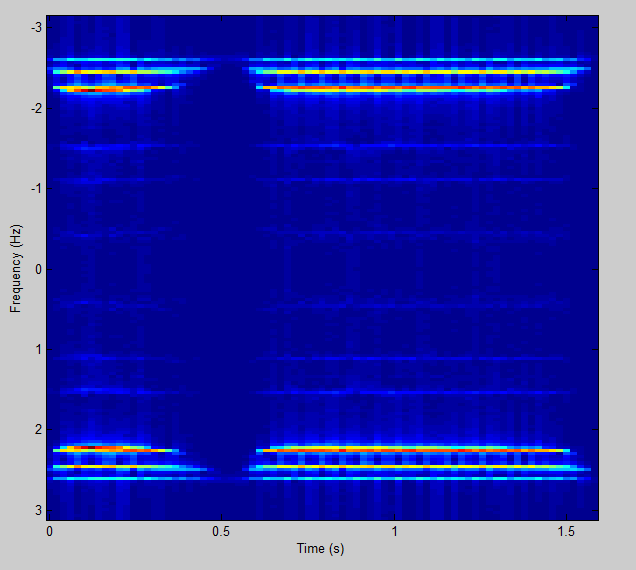
\includegraphics[scale = 0.7]{resources/labday1_report4_timefrequency.png}
\caption{Time-frequency plot.}
\label{fig:timefreq}
\end{figure}

\subsection{Report 5 \& 6}

Sometimes the resolution might not be very high. 
To address this issue we consider zero padding.
This is basically augmenting a signal with zeros.
Subsequently the original samples will be interpolated.
In figure \ref{fig:zeropadding} an amplitude spectrum is shown.
The circles point to a Fourier transformed impulse response without zero padding, while the pluses indicate that zero padding has been applied.
Interpolation is obtained as every 4th sample coincides with a sample of the non augmented impulse response.

\begin{figure}[H]
    \centering
	\setlength\figureheight{6cm}
    	\setlength\figurewidth{14cm}
	% This file was created by matlab2tikz v0.4.6 running on MATLAB 8.3.
% Copyright (c) 2008--2014, Nico Schlömer <nico.schloemer@gmail.com>
% All rights reserved.
% Minimal pgfplots version: 1.3
% 
% The latest updates can be retrieved from
%   http://www.mathworks.com/matlabcentral/fileexchange/22022-matlab2tikz
% where you can also make suggestions and rate matlab2tikz.
% 
\begin{tikzpicture}

\begin{axis}[%
width=\figurewidth,
height=\figureheight,
scale only axis,
xmin=0,
xmax=1,
xlabel={Frequency (Hz)},
ymin=0,
ymax=3,
ylabel={Amplitude}
]
\addplot [color=blue,only marks,mark=o,mark options={solid},forget plot]
  table[row sep=crcr]{
0	2.7	\\
0.0769230769230769	0.849045436113243	\\
0.153846153846154	2.49555226711168	\\
0.230769230769231	0.466566034269694	\\
0.307692307692308	1.92954967807022	\\
0.384615384615385	0.321656600909142	\\
0.461538461538462	1.13447429946454	\\
0.538461538461539	1.13447429946454	\\
0.615384615384615	0.321656600909142	\\
0.692307692307692	1.92954967807022	\\
0.769230769230769	0.466566034269694	\\
0.846153846153846	2.49555226711168	\\
0.923076923076923	0.849045436113243	\\
};
\addplot [color=blue,only marks,mark=+,mark options={solid},forget plot]
  table[row sep=crcr]{
0	2.7	\\
0.0192307692307692	2.25122933360484	\\
0.0384615384615385	1.13447429946454	\\
0.0576923076923077	0.205188696869487	\\
0.0769230769230769	0.849045436113243	\\
0.0961538461538462	0.700018622361898	\\
0.115384615384615	0.321656600909142	\\
0.134615384615385	1.54961370571638	\\
0.153846153846154	2.49555226711168	\\
0.173076923076923	2.64812785369316	\\
0.192307692307692	1.92954967807022	\\
0.211538461538462	0.711304609918332	\\
0.230769230769231	0.466566034269694	\\
0.25	0.9	\\
0.269230769230769	0.466566034269694	\\
0.288461538461538	0.711304609918332	\\
0.307692307692308	1.92954967807022	\\
0.326923076923077	2.64812785369316	\\
0.346153846153846	2.49555226711168	\\
0.365384615384615	1.54961370571638	\\
0.384615384615385	0.321656600909142	\\
0.403846153846154	0.700018622361898	\\
0.423076923076923	0.849045436113243	\\
0.442307692307692	0.205188696869487	\\
0.461538461538462	1.13447429946454	\\
0.480769230769231	2.25122933360484	\\
0.5	2.7	\\
0.519230769230769	2.25122933360484	\\
0.538461538461538	1.13447429946454	\\
0.557692307692308	0.205188696869487	\\
0.576923076923077	0.849045436113243	\\
0.596153846153846	0.700018622361898	\\
0.615384615384615	0.321656600909142	\\
0.634615384615385	1.54961370571638	\\
0.653846153846154	2.49555226711168	\\
0.673076923076923	2.64812785369316	\\
0.692307692307692	1.92954967807022	\\
0.711538461538461	0.711304609918332	\\
0.730769230769231	0.466566034269694	\\
0.75	0.9	\\
0.769230769230769	0.466566034269694	\\
0.788461538461538	0.711304609918332	\\
0.807692307692308	1.92954967807022	\\
0.826923076923077	2.64812785369316	\\
0.846153846153846	2.49555226711168	\\
0.865384615384615	1.54961370571638	\\
0.884615384615385	0.321656600909142	\\
0.903846153846154	0.700018622361898	\\
0.923076923076923	0.849045436113243	\\
0.942307692307692	0.205188696869487	\\
0.961538461538461	1.13447429946454	\\
0.980769230769231	2.25122933360484	\\
};
\addplot [color=red,solid,forget plot]
  table[row sep=crcr]{
0	2.7	\\
0.0192307692307692	2.25122933360484	\\
0.0384615384615385	1.13447429946454	\\
0.0576923076923077	0.205188696869487	\\
0.0769230769230769	0.849045436113243	\\
0.0961538461538462	0.700018622361898	\\
0.115384615384615	0.321656600909142	\\
0.134615384615385	1.54961370571638	\\
0.153846153846154	2.49555226711168	\\
0.173076923076923	2.64812785369316	\\
0.192307692307692	1.92954967807022	\\
0.211538461538462	0.711304609918332	\\
0.230769230769231	0.466566034269694	\\
0.25	0.9	\\
0.269230769230769	0.466566034269694	\\
0.288461538461538	0.711304609918332	\\
0.307692307692308	1.92954967807022	\\
0.326923076923077	2.64812785369316	\\
0.346153846153846	2.49555226711168	\\
0.365384615384615	1.54961370571638	\\
0.384615384615385	0.321656600909142	\\
0.403846153846154	0.700018622361898	\\
0.423076923076923	0.849045436113243	\\
0.442307692307692	0.205188696869487	\\
0.461538461538462	1.13447429946454	\\
0.480769230769231	2.25122933360484	\\
0.5	2.7	\\
0.519230769230769	2.25122933360484	\\
0.538461538461538	1.13447429946454	\\
0.557692307692308	0.205188696869487	\\
0.576923076923077	0.849045436113243	\\
0.596153846153846	0.700018622361898	\\
0.615384615384615	0.321656600909142	\\
0.634615384615385	1.54961370571638	\\
0.653846153846154	2.49555226711168	\\
0.673076923076923	2.64812785369316	\\
0.692307692307692	1.92954967807022	\\
0.711538461538461	0.711304609918332	\\
0.730769230769231	0.466566034269694	\\
0.75	0.9	\\
0.769230769230769	0.466566034269694	\\
0.788461538461538	0.711304609918332	\\
0.807692307692308	1.92954967807022	\\
0.826923076923077	2.64812785369316	\\
0.846153846153846	2.49555226711168	\\
0.865384615384615	1.54961370571638	\\
0.884615384615385	0.321656600909142	\\
0.903846153846154	0.700018622361898	\\
0.923076923076923	0.849045436113243	\\
0.942307692307692	0.205188696869487	\\
0.961538461538461	1.13447429946454	\\
0.980769230769231	2.25122933360484	\\
};
\addplot [color=blue,only marks,mark=o,mark options={solid},forget plot]
  table[row sep=crcr]{
0	2.7	\\
0.0769230769230769	0.849045436113243	\\
0.153846153846154	2.49555226711168	\\
0.230769230769231	0.466566034269694	\\
0.307692307692308	1.92954967807022	\\
0.384615384615385	0.321656600909142	\\
0.461538461538462	1.13447429946454	\\
0.538461538461539	1.13447429946454	\\
0.615384615384615	0.321656600909142	\\
0.692307692307692	1.92954967807022	\\
0.769230769230769	0.466566034269694	\\
0.846153846153846	2.49555226711168	\\
0.923076923076923	0.849045436113243	\\
};
\addplot [color=blue,only marks,mark=+,mark options={solid},forget plot]
  table[row sep=crcr]{
0	2.7	\\
0.0192307692307692	2.25122933360484	\\
0.0384615384615385	1.13447429946454	\\
0.0576923076923077	0.205188696869487	\\
0.0769230769230769	0.849045436113243	\\
0.0961538461538462	0.700018622361898	\\
0.115384615384615	0.321656600909142	\\
0.134615384615385	1.54961370571638	\\
0.153846153846154	2.49555226711168	\\
0.173076923076923	2.64812785369316	\\
0.192307692307692	1.92954967807022	\\
0.211538461538462	0.711304609918332	\\
0.230769230769231	0.466566034269694	\\
0.25	0.9	\\
0.269230769230769	0.466566034269694	\\
0.288461538461538	0.711304609918332	\\
0.307692307692308	1.92954967807022	\\
0.326923076923077	2.64812785369316	\\
0.346153846153846	2.49555226711168	\\
0.365384615384615	1.54961370571638	\\
0.384615384615385	0.321656600909142	\\
0.403846153846154	0.700018622361898	\\
0.423076923076923	0.849045436113243	\\
0.442307692307692	0.205188696869487	\\
0.461538461538462	1.13447429946454	\\
0.480769230769231	2.25122933360484	\\
0.5	2.7	\\
0.519230769230769	2.25122933360484	\\
0.538461538461538	1.13447429946454	\\
0.557692307692308	0.205188696869487	\\
0.576923076923077	0.849045436113243	\\
0.596153846153846	0.700018622361898	\\
0.615384615384615	0.321656600909142	\\
0.634615384615385	1.54961370571638	\\
0.653846153846154	2.49555226711168	\\
0.673076923076923	2.64812785369316	\\
0.692307692307692	1.92954967807022	\\
0.711538461538461	0.711304609918332	\\
0.730769230769231	0.466566034269694	\\
0.75	0.9	\\
0.769230769230769	0.466566034269694	\\
0.788461538461538	0.711304609918332	\\
0.807692307692308	1.92954967807022	\\
0.826923076923077	2.64812785369316	\\
0.846153846153846	2.49555226711168	\\
0.865384615384615	1.54961370571638	\\
0.884615384615385	0.321656600909142	\\
0.903846153846154	0.700018622361898	\\
0.923076923076923	0.849045436113243	\\
0.942307692307692	0.205188696869487	\\
0.961538461538461	1.13447429946454	\\
0.980769230769231	2.25122933360484	\\
};
\addplot [color=red,solid,forget plot]
  table[row sep=crcr]{
0	2.7	\\
0.0192307692307692	2.25122933360484	\\
0.0384615384615385	1.13447429946454	\\
0.0576923076923077	0.205188696869487	\\
0.0769230769230769	0.849045436113243	\\
0.0961538461538462	0.700018622361898	\\
0.115384615384615	0.321656600909142	\\
0.134615384615385	1.54961370571638	\\
0.153846153846154	2.49555226711168	\\
0.173076923076923	2.64812785369316	\\
0.192307692307692	1.92954967807022	\\
0.211538461538462	0.711304609918332	\\
0.230769230769231	0.466566034269694	\\
0.25	0.9	\\
0.269230769230769	0.466566034269694	\\
0.288461538461538	0.711304609918332	\\
0.307692307692308	1.92954967807022	\\
0.326923076923077	2.64812785369316	\\
0.346153846153846	2.49555226711168	\\
0.365384615384615	1.54961370571638	\\
0.384615384615385	0.321656600909142	\\
0.403846153846154	0.700018622361898	\\
0.423076923076923	0.849045436113243	\\
0.442307692307692	0.205188696869487	\\
0.461538461538462	1.13447429946454	\\
0.480769230769231	2.25122933360484	\\
0.5	2.7	\\
0.519230769230769	2.25122933360484	\\
0.538461538461538	1.13447429946454	\\
0.557692307692308	0.205188696869487	\\
0.576923076923077	0.849045436113243	\\
0.596153846153846	0.700018622361898	\\
0.615384615384615	0.321656600909142	\\
0.634615384615385	1.54961370571638	\\
0.653846153846154	2.49555226711168	\\
0.673076923076923	2.64812785369316	\\
0.692307692307692	1.92954967807022	\\
0.711538461538461	0.711304609918332	\\
0.730769230769231	0.466566034269694	\\
0.75	0.9	\\
0.769230769230769	0.466566034269694	\\
0.788461538461538	0.711304609918332	\\
0.807692307692308	1.92954967807022	\\
0.826923076923077	2.64812785369316	\\
0.846153846153846	2.49555226711168	\\
0.865384615384615	1.54961370571638	\\
0.884615384615385	0.321656600909142	\\
0.903846153846154	0.700018622361898	\\
0.923076923076923	0.849045436113243	\\
0.942307692307692	0.205188696869487	\\
0.961538461538461	1.13447429946454	\\
0.980769230769231	2.25122933360484	\\
};
\end{axis}
\end{tikzpicture}%
	\caption{The circles indicate no zero padding while the pluses do.}
	\label{fig:zeropadding}
\end{figure}

\subsection{Report 7}
To demonstrate the convolution property, as noted in equation \ref{eq:convolution}, $X(\omega)H(\omega)$ should be identical to $Y(\omega)$.
\begin{equation}
y[n] = x[n] * h[n] \Leftrightarrow Y(\omega) = X(\omega)H(\omega)
\label{eq:convolution}
\end{equation}
For this reason we convolute the vectors x and h to get an y. 
Afterwards we apply the Fourier transform on y.
Parallel to this x and h are Fourier transformed after which they are multiplied.
This should result in identical plots.
For the latter case x and h should have the length of y.
To obtain the right length we make use of zero padding.
In figure \ref{fig:convolution} the two plots are identical and thus the convolution property is demonstrated.

\begin{figure}[H]
    \centering
	\setlength\figureheight{6cm}
    	\setlength\figurewidth{14cm}
	% This file was created by matlab2tikz v0.4.6 running on MATLAB 8.3.
% Copyright (c) 2008--2014, Nico Schlömer <nico.schloemer@gmail.com>
% All rights reserved.
% Minimal pgfplots version: 1.3
% 
% The latest updates can be retrieved from
%   http://www.mathworks.com/matlabcentral/fileexchange/22022-matlab2tikz
% where you can also make suggestions and rate matlab2tikz.
% 
\begin{tikzpicture}

\begin{axis}[%
width=\figurewidth,
height=\figureheight,
scale only axis,
xmin=-3.14159265358979,
xmax=3.14114301960474,
ymin=0,
ymax=2500,
name=plot1
]
\addplot [color=blue,solid,forget plot]
  table[row sep=crcr]{
-3.14159265358979	19.8926584456553	\\
-3.12675473208293	0.0532087870446882	\\
-3.11911095433697	2.57064553821331	\\
-3.11101754260595	1.27544115516442	\\
-3.10517230080022	0.012485403205535	\\
-3.08943511132324	1.91644737522381	\\
-3.08538840545773	0.212474242094612	\\
-3.08314023553245	0.0838492963971151	\\
-3.07234901989109	2.49722134003265	\\
-3.06830231402558	0.0962186821635277	\\
-3.05706146439917	1.72924839592516	\\
-3.0485184186831	1.66281160520585	\\
-3.04627024875781	0.127820081329008	\\
-3.03098269326589	0.0706835516622831	\\
-3.02603671943027	1.86093549827026	\\
-3.02333891551993	0.161773970788943	\\
-3.02154037957971	1.38923085606008	\\
-3.00355502017745	3.01650899809105	\\
-3.00040758228205	0.216074057948433	\\
-2.99141490258092	0.0367743314174455	\\
-2.98197258889473	1.77238192397133	\\
-2.97972441896945	2.41393860297375	\\
-2.97118137325338	0.0928657729370627	\\
-2.95724271971663	2.0902597787146	\\
-2.95364564783617	0.0282881474970191	\\
-2.9451026021201	0.117811171829853	\\
-2.94060626226954	1.60211367575097	\\
-2.93655955640403	0.0333338621943806	\\
-2.92711724271784	5.25965848044103	\\
-2.92396980482245	4.23078513885601	\\
-2.91587639309143	0.118069256589241	\\
-2.90823261534547	0.124401303364409	\\
-2.90598444542018	4.3862467870769	\\
-2.88889835398804	3.58747122572868	\\
-2.88530128210759	0.150608405431404	\\
-2.88080494225702	1.49326518519667	\\
-2.87540933443634	0.0252196185317378	\\
-2.8655173867651	2.27296335694572	\\
-2.86147068089959	0.12693446657177	\\
-2.84933056330307	2.56642618414948	\\
-2.83898898164677	0.0643457918178676	\\
-2.83089556991575	0.128446439925093	\\
-2.82639923006518	2.21339228450317	\\
-2.82145325622956	0.107161458215456	\\
-2.81875545231922	3.61938596000812	\\
-2.80166936088708	0.0188790899191806	\\
-2.79582411908134	2.90312861041924	\\
-2.79402558314112	0.210704076393256	\\
-2.78098619757448	3.05206849108307	\\
-2.77514095576874	3.14897397933414	\\
-2.77019498193312	0.00153586525415124	\\
-2.76030303426188	0.190128689478314	\\
-2.7517599885458	2.03384603580528	\\
-2.74681401471018	0.0771736221028695	\\
-2.74366657681479	2.01446283056626	\\
-2.73287536117343	2.32433014135083	\\
-2.72478194944241	0.0940196992389875	\\
-2.71533963575623	0.145533812642321	\\
-2.71084329590566	2.72575122386714	\\
-2.70544768808498	2.42779957625067	\\
-2.70274988417465	0.0734579525711054	\\
-2.68521415875744	0.0462058253577377	\\
-2.6825163548471	4.05199063103163	\\
-2.67622147905631	3.35656895436007	\\
-2.66857770131035	0.144612236845544	\\
-2.65958502160922	3.46435485198692	\\
-2.64969307393798	0.0360835363255782	\\
-2.64924343995292	0.42984603117975	\\
-2.63485515243111	8.82579083502318	\\
-2.62721137468515	0.564476074568702	\\
-2.62001723092425	49.9399519297817	\\
-2.60967564926795	5.04787971905156	\\
-2.60652821137255	241.563377121866	\\
-2.60158223753693	410.306944561965	\\
-2.59348882580592	2.39071400449906	\\
-2.59034138791052	13.1669073905317	\\
-2.57685236835882	0.284559849196704	\\
-2.57595310038871	0.149368125229052	\\
-2.57370493046343	7.28455897645908	\\
-2.56066554489679	5.33033992568238	\\
-2.55392103512094	0.230489414552615	\\
-2.54492835541981	6.44038442499614	\\
-2.54043201556925	0.33703182457791	\\
-2.53098970188306	0.189490523276336	\\
-2.52199702218193	8.72813803699814	\\
-2.51795031631642	0.304868032518704	\\
-2.50491093074978	21.1624892630286	\\
-2.49636788503371	27.9830091157402	\\
-2.49591825104865	0.727890114091731	\\
-2.48467740142224	3.76176580377005	\\
-2.47658398969122	165.53867903062	\\
-2.47208764984066	19.8929677550075	\\
-2.4644438720947	492.986662568109	\\
-2.45949789825908	585.133990276727	\\
-2.44825704863266	0.432385168545974	\\
-2.43926436893153	0.454501772797956	\\
-2.4365665650212	15.9468842395576	\\
-2.42847315329018	15.979168879326	\\
-2.42577534937984	0.137044810441969	\\
-2.41003815990286	0.223978183776946	\\
-2.40644108802241	16.5498674043315	\\
-2.40284401614196	0.519622744440768	\\
-2.39025426456038	9.74483230277733	\\
-2.38350975478453	12.8167756750116	\\
-2.38036231688913	0.559236167527878	\\
-2.37092000320295	0.430379161123992	\\
-2.36147768951676	7.59222635706518	\\
-2.35698134966619	0.108118890436206	\\
-2.35428354575585	9.93512366979884	\\
-2.33854635627888	11.4656761149616	\\
-2.33180184650303	1.0287496436849	\\
-2.32820477462258	0.338504212020415	\\
-2.32056099687662	16.7183720096503	\\
-2.31471575507088	23.5207211339421	\\
-2.3052734413847	1.44956711035969	\\
-2.29223405581806	54.8185618571025	\\
-2.28818734995255	1.61102489167945	\\
-2.27964430423648	4.23862174118417	\\
-2.2742486964158	106.167950884941	\\
-2.26885308859512	182.22370137463	\\
-2.25851150693882	6.06144052992204	\\
-2.24502248738712	2476.13546958913	\\
-2.24367358543195	1013.98945314128	\\
-2.23243273580554	6.83375636334474	\\
-2.22883566392509	52.0515388884008	\\
-2.21894371625385	1.39709458450789	\\
-2.20725323264238	20.2476741076976	\\
-2.20320652677687	1.15512796207575	\\
-2.20005908888147	15.6909148150422	\\
-2.18657006932978	0.403730777514918	\\
-2.17532921970337	27.6473672346279	\\
-2.17263141579303	0.720286869288151	\\
-2.16633654000224	0.734390437905012	\\
-2.15914239624133	18.5528372629984	\\
-2.15374678842065	13.8916730146768	\\
-2.1501497165402	0.653642562814454	\\
-2.14070740285402	0.169766100504169	\\
-2.13755996495862	12.7697069806375	\\
-2.11732643563108	0.549272029838374	\\
-2.11597753367591	5.89962358806633	\\
-2.10788412194489	13.7634577359606	\\
-2.10338778209433	0.349053686772005	\\
-2.0943951023932	0.210274044405798	\\
-2.08989876254263	7.94066866383391	\\
-2.0840535207369	8.14342146687816	\\
-2.07191340314037	0.197401818828818	\\
-2.06157182148407	26.1718804663576	\\
-2.05842438358868	0.773915104326615	\\
-2.05527694569328	8.79359719167923	\\
-2.04853243591743	0.189862054928003	\\
-2.03504341636574	0.237143504436913	\\
-2.0323456124554	4.99066752537407	\\
-2.0220040307991	0.0956697335516264	\\
-2.02110476282899	4.92125576897894	\\
-2.00266976944167	0.0774503957368301	\\
-1.99952233154627	7.45371945192958	\\
-1.99772379560605	4.6006647382492	\\
-1.98918074988997	0.12749680707944	\\
-1.97973843620379	0.146787854193875	\\
-1.96939685454749	6.35453068734138	\\
-1.96849758657737	4.20319594474824	\\
-1.96265234477164	0.0807702240775046	\\
-1.94736478927972	3.74503331278603	\\
-1.94331808341421	0.0761937905147443	\\
-1.93342613574297	0.0302204524480887	\\
-1.92982906386252	4.2749282586906	\\
-1.92398382205678	5.68451894520705	\\
-1.92038675017633	0.283028327672143	\\
-1.91049480250509	0.123428201161085	\\
-1.90734736460969	4.54386895558947	\\
-1.8875634692672	0.102016699557211	\\
-1.88396639738675	4.48080262933705	\\
-1.87947005753619	4.35571560129846	\\
-1.87407444971551	0.178555934936627	\\
-1.86463213602932	0.0685195298608476	\\
-1.85384092038797	3.92418099057164	\\
-1.84170080279144	0.0268939699058458	\\
-1.83945263286616	4.62584030444586	\\
-1.83855336489604	4.15839707868827	\\
-1.8286614172248	0.074279113519074	\\
-1.81876946955356	0.0750306472233845	\\
-1.80977678985243	4.07065149183564	\\
-1.80842788789726	3.48512804005471	\\
-1.79583813631568	0.0427814343622637	\\
-1.78954326052489	0.365363633867683	\\
-1.78504692067432	16.016713380486	\\
-1.77830241089847	7.11393971060506	\\
-1.7729068030778	0.278726905174866	\\
-1.76211558743644	3.68904740694711	\\
-1.7594177835261	0.0746234355896293	\\
-1.74592876397441	5.00468214258017	\\
-1.74323096006407	0.16296470437005	\\
-1.73648645028822	0.0468474515857732	\\
-1.72254779675147	2.88233537524637	\\
-1.7180514569009	5.54455975910776	\\
-1.71400475103539	0.141959094005153	\\
-1.70366316937909	0.0554711875012217	\\
-1.70006609749864	4.71499163350529	\\
-1.69287195373774	3.39774808833229	\\
-1.68073183614121	0.082190368128078	\\
-1.67578586230559	6.35359175314588	\\
-1.66769245057457	0.190171800012267	\\
-1.65780050290333	0.0709065378871592	\\
-1.6560019669631	8.9570059818486	\\
-1.64745892124703	12.9226088121107	\\
-1.64476111733669	0.28725170218465	\\
-1.63486916966545	0.0209794613833366	\\
-1.63217136575511	8.41082156820344	\\
-1.61193783642757	0.0977324817758621	\\
-1.60879039853217	14.032888311883	\\
-1.60654222860689	10.6541498279629	\\
-1.59844881687587	0.286813108722075	\\
-1.58900650318968	0.293239032341302	\\
-1.58630869927935	21.7217540403053	\\
-1.57596711762305	0.0654171936989979	\\
-1.56382700002652	18.4826848804303	\\
-1.5588810261909	0.700755695098959	\\
-1.55528395431045	25.3010275374739	\\
-1.54808981054954	1.06558784718216	\\
-1.53864749686336	40.4197337709948	\\
-1.53010445114728	0.660976059794117	\\
-1.52246067340132	111.4625235256	\\
-1.51166945775997	91.1529537651241	\\
-1.50672348392434	0.235685205812729	\\
-1.49952934016344	25.8384254852915	\\
-1.49638190226805	0.282315541283869	\\
-1.48693958858186	24.3182308636348	\\
-1.48379215068646	0.644918188313327	\\
-1.47434983700028	0.660724444002167	\\
-1.47030313113477	12.1584709253588	\\
-1.45096886977734	0.149429691982144	\\
-1.44782143188194	6.27675810845753	\\
-1.44602289594172	8.78460013554648	\\
-1.43703021624059	0.271748147190503	\\
-1.42803753653946	0.220751682035347	\\
-1.424440464659	7.71063611254086	\\
-1.41859522285327	7.47958593051218	\\
-1.41499815097282	0.180020898684117	\\
-1.40285803337629	10.2314632616844	\\
-1.40150913142112	0.118701543739853	\\
-1.38127560209358	0.238693595014367	\\
-1.38037633412347	10.7037387112309	\\
-1.36913548449705	0.0188655951495292	\\
-1.36104207276604	9.1028081624014	\\
-1.35924353682581	0.403148375165112	\\
-1.34755305321434	28.0905820761561	\\
-1.34440561531895	0.57527786401742	\\
-1.33316476569253	16.2832434531534	\\
-1.33181586373736	10.7515234651398	\\
-1.32282318403623	0.0546328682440252	\\
-1.31338087035005	0.0942097225965186	\\
-1.30303928869375	8.9321424859863	\\
-1.28999990312711	0.0735324312574333	\\
-1.28775173320183	5.84009946538904	\\
-1.28370502733632	0.117807301005373	\\
-1.27066564176968	0.0972705818588063	\\
-1.26482039996395	6.23505810243354	\\
-1.25942479214327	4.10387246584359	\\
-1.25402918432259	0.0355173616024903	\\
-1.24503650462146	0.249650943925795	\\
-1.24009053078584	4.35538475815771	\\
-1.22120590341346	0.182006403034195	\\
-1.21760883153301	7.24358599396274	\\
-1.21176358972728	5.82064118678822	\\
-1.20681761589166	0.226991257713179	\\
-1.19827457017558	0.539531648837398	\\
-1.19467749829513	10.228883933073	\\
-1.1784906748331	7.06030676064892	\\
-1.17624250490781	0.156336414770753	\\
-1.1650016552814	8.71934224821784	\\
-1.16230385137106	0.208430751324701	\\
-1.15286153768488	0.255527236054257	\\
-1.14971409978948	15.5596527030979	\\
-1.14207032204352	12.5816725721892	\\
-1.13892288414812	0.222072667434679	\\
-1.12408496264126	31.8124416056185	\\
-1.12183679271598	0.437660871933631	\\
-1.10744850519417	1.63740204294597	\\
-1.10250253135855	240.523702212192	\\
-1.09665728955281	52.8705447260934	\\
-1.08586607391146	1.72584526169728	\\
-1.08451717195629	0.651574085317387	\\
-1.07372595631493	19.0603023354286	\\
-1.07012888443448	0.255184262823433	\\
-1.05798876683795	9.25825358128747	\\
-1.05484132894256	0.598948654264419	\\
-1.05124425706211	9.49877816333689	\\
-1.03101072773456	0.208939010776117	\\
-1.02831292382422	12.3179050320662	\\
-1.01797134216792	5.44305892729178	\\
-1.01482390427253	0.459515040520143	\\
-1.01032756442196	17.1172038797662	\\
-1.00088525073578	0.259124489500461	\\
-0.996838544870269	0.291999842737283	\\
-0.987845865169139	11.802405515419	\\
-0.983349525318574	5.81562217527288	\\
-0.97750428351284	0.130358097585567	\\
-0.968061969826653	0.082340108109789	\\
-0.963115995991032	5.84366157089055	\\
-0.955022584260015	0.0702963892319461	\\
-0.941083930723263	5.11028380092381	\\
-0.932540885007189	0.108803297400991	\\
-0.922648937335946	0.370608775198911	\\
-0.919051865455494	6.0074553421597	\\
-0.905113211918743	0.10698723546407	\\
-0.897469434172782	6.3642154214645	\\
-0.88622858454637	0.218420546540637	\\
-0.876786270860183	0.249054060468997	\\
-0.873638832964788	6.39969945840234	\\
-0.863297251308488	0.247563216350043	\\
-0.856103107547584	6.45955227983675	\\
-0.850257865741849	6.49052127704355	\\
-0.840365918070606	0.214449183592143	\\
-0.830923604384419	0.309826053382562	\\
-0.828675434459137	6.54115990189622	\\
-0.820132388743063	2.62955605789736	\\
-0.813387878967216	0.0355907240214964	\\
-0.808441905131594	0.0670105912474191	\\
-0.805744101221255	4.93293718019949	\\
-0.7846113039236	0.0365951810973887	\\
-0.78191350001326	4.30432597361454	\\
-0.775618624222469	5.52893272832956	\\
-0.772021552342018	0.436938417722433	\\
-0.764377774596057	4.25188963121735	\\
-0.753586558954701	0.153758612803091	\\
-0.743694611283458	0.226560192844928	\\
-0.741896075343232	3.65355650402903	\\
-0.728856689776593	5.50186116376013	\\
-0.725259617896141	0.430002820634587	\\
-0.715817304209954	0.110207185854368	\\
-0.714018768269729	5.64307291122997	\\
-0.706374990523768	7.17083238821062	\\
-0.703227552628372	0.226992840528917	\\
-0.689738533076677	0.0781777717468108	\\
-0.689288899091621	6.09191027381145	\\
-0.678048049465208	0.199236321363024	\\
-0.665907931868682	6.71049915763951	\\
-0.662310859988231	0.344252916824491	\\
-0.659613056077891	6.72434110868123	\\
-0.647023304496309	0.361076953307015	\\
-0.638030624795179	5.62343067291799	\\
-0.636232088854953	5.12361480545967	\\
-0.633084650959558	0.209131575006773	\\
-0.620045265392919	8.02122986699579	\\
-0.610602951706733	0.475146655222324	\\
-0.601160638020546	0.436265881703127	\\
-0.597113932155037	8.09618061069338	\\
-0.591718324334359	9.43462213356189	\\
-0.580477474707947	0.157104023421555	\\
-0.573283330947043	8.93914002740303	\\
-0.564740285230969	0.152139142849741	\\
-0.550351997709161	8.07508192323586	\\
-0.545406023873539	8.65280691066647	\\
-0.541808951993088	0.584091572937608	\\
-0.527870298456336	14.0700639340484	\\
-0.524273226575884	0.178777674974315	\\
-0.514830912889697	0.731631390134797	\\
-0.507187135143737	7.39062775239001	\\
-0.499992991382832	16.4936521005183	\\
-0.495946285517324	1.11473101140068	\\
-0.486503971831137	1.32448791015046	\\
-0.482457265965629	23.3986449873541	\\
-0.475712756189781	27.6795569756248	\\
-0.474813488219668	0.475744951951137	\\
-0.462673370623143	2.0960773391043	\\
-0.4527814229519	51.7867280080287	\\
-0.444688011220883	1.05865098700483	\\
-0.437943501445035	42.0928838079822	\\
-0.430749357684131	36.9311768297169	\\
-0.426702651818622	0.515291527572411	\\
-0.41411290023704	33.5573356924844	\\
-0.410515828356588	0.395447548758222	\\
-0.403771318580741	1.29667402693208	\\
-0.391181566999159	15.8290642070355	\\
-0.389832665043989	27.6274800231544	\\
-0.377242913462407	1.28736203229961	\\
-0.375444377522181	20.1649259779998	\\
-0.371397671656672	2.33262879157686	\\
-0.361505723985429	14.8191930587707	\\
-0.348016704433734	0.604342762466176	\\
-0.341272194657887	0.477171926523295	\\
-0.338124756762491	13.7181008208293	\\
-0.323736469240683	0.0634528301774847	\\
-0.322387567285514	9.47287770413512	\\
-0.316542325479779	8.79131361261518	\\
-0.312045985629214	0.611935683659901	\\
-0.302154037957971	0.230086716936798	\\
-0.297657698107406	10.0858880685462	\\
-0.278773070735033	0.601671674176026	\\
-0.276974534794807	10.3801846251015	\\
-0.274276730884468	11.4759256230187	\\
-0.271129292989072	0.720670297543253	\\
-0.253143933586812	13.0511753102932	\\
-0.252244665616699	0.272894872887547	\\
-0.236957110124778	0.0688344029671348	\\
-0.236057842154665	5.08395985277606	\\
-0.229762966363874	7.29623724844187	\\
-0.220320652677687	0.138001054348589	\\
-0.206381999140935	6.40210038923912	\\
-0.20323456124554	0.172517564857273	\\
-0.197838953424862	0.294857014891671	\\
-0.189745541693845	3.9799361479004	\\
-0.187047737783506	0.0637000187503415	\\
-0.183450665903054	6.19420820545885	\\
-0.169961646351358	0.205181356843812	\\
-0.161868234620342	4.23956348029029	\\
-0.152875554919211	2.82161838287159	\\
-0.151976286949099	0.192417664670228	\\
-0.142084339277855	0.0282934343198709	\\
-0.138037633412347	5.39676833979871	\\
-0.129494587696273	2.50760534042733	\\
-0.127696051756047	0.0933586920275544	\\
-0.115106300174465	2.72517227484558	\\
-0.105663986488278	0.0714281588344531	\\
-0.0984698427273747	0.128850734872603	\\
-0.0926246009216398	2.7695015485174	\\
-0.0777866794147752	0.187643878288714	\\
-0.0755385094894927	2.97654141208107	\\
-0.0683443657285889	1.73845254928587	\\
-0.0660961958033064	0.0194202524749926	\\
-0.0553049801619503	0.0427546446086761	\\
-0.051707908281498	2.28863913103362	\\
-0.043614496550481	1.26335580136522	\\
-0.0422655945953117	0.132332292338383	\\
-0.0215824312827122	0.216440371596831	\\
-0.0170860914321471	3.21492506903341	\\
-0.00449633985056508	0.0778995026941969	\\
-4.44089209850063e-16	5.09414969888162	\\
0.00449633985056463	0.0778995026941969	\\
0.0170860914321467	3.21492506903341	\\
0.0215824312827118	0.216440371596831	\\
0.0422655945953108	0.132332292338383	\\
0.0436144965504806	1.26335580136522	\\
0.0517079082814975	2.28863913103362	\\
0.0553049801619494	0.0427546446086761	\\
0.0660961958033055	0.0194202524749926	\\
0.068344365728588	1.73845254928587	\\
0.0755385094894923	2.97654141208107	\\
0.0777866794147748	0.187643878288714	\\
0.0926246009216394	2.7695015485174	\\
0.0984698427273738	0.128850734872603	\\
0.105663986488278	0.0714281588344531	\\
0.115106300174465	2.72517227484558	\\
0.127696051756047	0.0933586920275544	\\
0.129494587696273	2.50760534042733	\\
0.138037633412346	5.39676833979871	\\
0.142084339277855	0.0282934343198709	\\
0.151976286949098	0.192417664670228	\\
0.152875554919211	2.82161838287159	\\
0.161868234620341	4.23956348029029	\\
0.169961646351358	0.205181356843812	\\
0.183450665903053	6.19420820545885	\\
0.187047737783505	0.0637000187503415	\\
0.189745541693844	3.9799361479004	\\
0.197838953424861	0.294857014891671	\\
0.20323456124554	0.172517564857273	\\
0.206381999140935	6.40210038923912	\\
0.220320652677687	0.138001054348589	\\
0.229762966363873	7.29623724844187	\\
0.236057842154664	5.08395985277606	\\
0.236957110124777	0.0688344029671348	\\
0.252244665616698	0.272894872887547	\\
0.253143933586812	13.0511753102932	\\
0.271129292989071	0.720670297543253	\\
0.274276730884467	11.4759256230187	\\
0.276974534794806	10.3801846251015	\\
0.278773070735032	0.601671674176026	\\
0.297657698107405	10.0858880685462	\\
0.30215403795797	0.230086716936798	\\
0.312045985629213	0.611935683659901	\\
0.316542325479778	8.79131361261518	\\
0.322387567285513	9.47287770413512	\\
0.323736469240683	0.0634528301774847	\\
0.338124756762491	13.7181008208293	\\
0.341272194657886	0.477171926523295	\\
0.348016704433733	0.604342762466176	\\
0.361505723985429	14.8191930587707	\\
0.371397671656672	2.33262879157686	\\
0.375444377522181	20.1649259779998	\\
0.377242913462406	1.28736203229961	\\
0.389832665043989	27.6274800231544	\\
0.391181566999158	15.8290642070355	\\
0.40377131858074	1.29667402693208	\\
0.410515828356588	0.395447548758222	\\
0.41411290023704	33.5573356924844	\\
0.426702651818622	0.515291527572411	\\
0.43074935768413	36.9311768297169	\\
0.437943501445035	42.0928838079822	\\
0.444688011220882	1.05865098700483	\\
0.452781422951899	51.7867280080287	\\
0.462673370623142	2.0960773391043	\\
0.474813488219668	0.475744951951137	\\
0.475712756189781	27.6795569756248	\\
0.482457265965628	23.3986449873541	\\
0.486503971831137	1.32448791015046	\\
0.495946285517324	1.11473101140068	\\
0.499992991382832	16.4936521005183	\\
0.507187135143736	7.39062775239001	\\
0.514830912889697	0.731631390134797	\\
0.524273226575883	0.178777674974315	\\
0.527870298456335	14.0700639340484	\\
0.541808951993087	0.584091572937608	\\
0.545406023873539	8.65280691066647	\\
0.55035199770916	8.07508192323586	\\
0.564740285230969	0.152139142849741	\\
0.573283330947042	8.93914002740303	\\
0.580477474707946	0.157104023421555	\\
0.591718324334359	9.43462213356189	\\
0.597113932155037	8.09618061069338	\\
0.601160638020545	0.436265881703127	\\
0.610602951706732	0.475146655222324	\\
0.620045265392918	8.02122986699579	\\
0.633084650959557	0.209131575006773	\\
0.636232088854953	5.12361480545967	\\
0.638030624795179	5.62343067291799	\\
0.647023304496309	0.361076953307015	\\
0.659613056077891	6.72434110868123	\\
0.66231085998823	0.344252916824491	\\
0.665907931868682	6.71049915763951	\\
0.678048049465207	0.199236321363024	\\
0.68928889909162	6.09191027381145	\\
0.689738533076677	0.0781777717468108	\\
0.703227552628372	0.226992840528917	\\
0.706374990523767	7.17083238821062	\\
0.714018768269728	5.64307291122997	\\
0.715817304209954	0.110207185854368	\\
0.72525961789614	0.430002820634587	\\
0.728856689776593	5.50186116376013	\\
0.741896075343231	3.65355650402903	\\
0.743694611283457	0.226560192844928	\\
0.7535865589547	0.153758612803091	\\
0.764377774596056	4.25188963121735	\\
0.772021552342017	0.436938417722433	\\
0.775618624222469	5.52893272832956	\\
0.78191350001326	4.30432597361454	\\
0.784611303923599	0.0365951810973887	\\
0.805744101221255	4.93293718019949	\\
0.808441905131594	0.0670105912474191	\\
0.813387878967215	0.0355907240214964	\\
0.820132388743063	2.62955605789736	\\
0.828675434459136	6.54115990189622	\\
0.830923604384419	0.309826053382562	\\
0.840365918070606	0.214449183592143	\\
0.850257865741848	6.49052127704355	\\
0.856103107547583	6.45955227983675	\\
0.863297251308487	0.247563216350043	\\
0.873638832964787	6.39969945840234	\\
0.876786270860182	0.249054060468997	\\
0.886228584546369	0.218420546540637	\\
0.897469434172781	6.3642154214645	\\
0.905113211918742	0.10698723546407	\\
0.919051865455494	6.0074553421597	\\
0.922648937335946	0.370608775198911	\\
0.932540885007189	0.108803297400991	\\
0.941083930723263	5.11028380092381	\\
0.955022584260014	0.0702963892319461	\\
0.963115995991031	5.84366157089055	\\
0.968061969826652	0.082340108109789	\\
0.97750428351284	0.130358097585567	\\
0.983349525318573	5.81562217527288	\\
0.987845865169138	11.802405515419	\\
0.996838544870268	0.291999842737283	\\
1.00088525073578	0.259124489500461	\\
1.01032756442196	17.1172038797662	\\
1.01482390427253	0.459515040520143	\\
1.01797134216792	5.44305892729178	\\
1.02831292382422	12.3179050320662	\\
1.03101072773456	0.208939010776117	\\
1.05124425706211	9.49877816333689	\\
1.05484132894256	0.598948654264419	\\
1.05798876683795	9.25825358128747	\\
1.07012888443448	0.255184262823433	\\
1.07372595631493	19.0603023354286	\\
1.08451717195629	0.651574085317387	\\
1.08586607391146	1.72584526169728	\\
1.09665728955281	52.8705447260934	\\
1.10250253135855	240.523702212192	\\
1.10744850519417	1.63740204294597	\\
1.12183679271598	0.437660871933631	\\
1.12408496264126	31.8124416056185	\\
1.13892288414812	0.222072667434679	\\
1.14207032204352	12.5816725721892	\\
1.14971409978948	15.5596527030979	\\
1.15286153768488	0.255527236054257	\\
1.16230385137106	0.208430751324701	\\
1.1650016552814	8.71934224821784	\\
1.17624250490781	0.156336414770753	\\
1.1784906748331	7.06030676064892	\\
1.19467749829513	10.228883933073	\\
1.19827457017558	0.539531648837398	\\
1.20681761589166	0.226991257713179	\\
1.21176358972728	5.82064118678822	\\
1.21760883153301	7.24358599396274	\\
1.22120590341346	0.182006403034195	\\
1.24009053078584	4.35538475815771	\\
1.24503650462146	0.249650943925795	\\
1.25402918432259	0.0355173616024903	\\
1.25942479214327	4.10387246584359	\\
1.26482039996394	6.23505810243354	\\
1.27066564176968	0.0972705818588063	\\
1.28370502733632	0.117807301005373	\\
1.28775173320183	5.84009946538904	\\
1.28999990312711	0.0735324312574333	\\
1.30303928869375	8.9321424859863	\\
1.31338087035005	0.0942097225965186	\\
1.32282318403623	0.0546328682440252	\\
1.33181586373736	10.7515234651398	\\
1.33316476569253	16.2832434531534	\\
1.34440561531895	0.57527786401742	\\
1.34755305321434	28.0905820761561	\\
1.35924353682581	0.403148375165112	\\
1.36104207276604	9.1028081624014	\\
1.36913548449705	0.0188655951495292	\\
1.38037633412347	10.7037387112309	\\
1.38127560209358	0.238693595014367	\\
1.40150913142112	0.118701543739853	\\
1.40285803337629	10.2314632616844	\\
1.41499815097282	0.180020898684117	\\
1.41859522285327	7.47958593051218	\\
1.424440464659	7.71063611254086	\\
1.42803753653946	0.220751682035347	\\
1.43703021624059	0.271748147190503	\\
1.44602289594172	8.78460013554648	\\
1.44782143188194	6.27675810845753	\\
1.45096886977734	0.149429691982144	\\
1.47030313113477	12.1584709253588	\\
1.47434983700028	0.660724444002167	\\
1.48379215068646	0.644918188313327	\\
1.48693958858186	24.3182308636348	\\
1.49638190226804	0.282315541283869	\\
1.49952934016344	25.8384254852915	\\
1.50672348392434	0.235685205812729	\\
1.51166945775997	91.1529537651241	\\
1.52246067340132	111.4625235256	\\
1.53010445114728	0.660976059794117	\\
1.53864749686336	40.4197337709948	\\
1.54808981054954	1.06558784718216	\\
1.55528395431045	25.3010275374739	\\
1.5588810261909	0.700755695098959	\\
1.56382700002652	18.4826848804303	\\
1.57596711762305	0.0654171936989979	\\
1.58630869927935	21.7217540403053	\\
1.58900650318968	0.293239032341302	\\
1.59844881687587	0.286813108722075	\\
1.60654222860689	10.6541498279629	\\
1.60879039853217	14.032888311883	\\
1.61193783642757	0.0977324817758621	\\
1.63217136575511	8.41082156820344	\\
1.63486916966545	0.0209794613833366	\\
1.64476111733669	0.28725170218465	\\
1.64745892124703	12.9226088121107	\\
1.6560019669631	8.9570059818486	\\
1.65780050290333	0.0709065378871592	\\
1.66769245057457	0.190171800012267	\\
1.67578586230559	6.35359175314588	\\
1.68073183614121	0.082190368128078	\\
1.69287195373774	3.39774808833229	\\
1.70006609749864	4.71499163350529	\\
1.70366316937909	0.0554711875012217	\\
1.71400475103539	0.141959094005153	\\
1.7180514569009	5.54455975910776	\\
1.72254779675147	2.88233537524637	\\
1.73648645028822	0.0468474515857732	\\
1.74323096006407	0.16296470437005	\\
1.7459287639744	5.00468214258017	\\
1.7594177835261	0.0746234355896293	\\
1.76211558743644	3.68904740694711	\\
1.77290680307779	0.278726905174866	\\
1.77830241089847	7.11393971060506	\\
1.78504692067432	16.016713380486	\\
1.78954326052489	0.365363633867683	\\
1.79583813631568	0.0427814343622637	\\
1.80842788789726	3.48512804005471	\\
1.80977678985243	4.07065149183564	\\
1.81876946955356	0.0750306472233845	\\
1.8286614172248	0.074279113519074	\\
1.83855336489604	4.15839707868827	\\
1.83945263286616	4.62584030444586	\\
1.84170080279144	0.0268939699058458	\\
1.85384092038796	3.92418099057164	\\
1.86463213602932	0.0685195298608476	\\
1.87407444971551	0.178555934936627	\\
1.87947005753619	4.35571560129846	\\
1.88396639738675	4.48080262933705	\\
1.8875634692672	0.102016699557211	\\
1.90734736460969	4.54386895558947	\\
1.91049480250508	0.123428201161085	\\
1.92038675017633	0.283028327672143	\\
1.92398382205678	5.68451894520705	\\
1.92982906386251	4.2749282586906	\\
1.93342613574297	0.0302204524480887	\\
1.94331808341421	0.0761937905147443	\\
1.94736478927972	3.74503331278603	\\
1.96265234477164	0.0807702240775046	\\
1.96849758657737	4.20319594474824	\\
1.96939685454749	6.35453068734138	\\
1.97973843620379	0.146787854193875	\\
1.98918074988997	0.12749680707944	\\
1.99772379560605	4.6006647382492	\\
1.99952233154627	7.45371945192958	\\
2.00266976944167	0.0774503957368301	\\
2.02110476282899	4.92125576897894	\\
2.0220040307991	0.0956697335516264	\\
2.0323456124554	4.99066752537407	\\
2.03504341636574	0.237143504436913	\\
2.04853243591743	0.189862054928003	\\
2.05527694569328	8.79359719167923	\\
2.05842438358867	0.773915104326615	\\
2.06157182148407	26.1718804663576	\\
2.07191340314037	0.197401818828818	\\
2.0840535207369	8.14342146687816	\\
2.08989876254263	7.94066866383391	\\
2.09439510239319	0.210274044405798	\\
2.10338778209433	0.349053686772005	\\
2.10788412194489	13.7634577359606	\\
2.11597753367591	5.89962358806633	\\
2.11732643563108	0.549272029838374	\\
2.13755996495862	12.7697069806375	\\
2.14070740285402	0.169766100504169	\\
2.1501497165402	0.653642562814454	\\
2.15374678842065	13.8916730146768	\\
2.15914239624133	18.5528372629984	\\
2.16633654000224	0.734390437905012	\\
2.17263141579303	0.720286869288151	\\
2.17532921970337	27.6473672346279	\\
2.18657006932978	0.403730777514918	\\
2.20005908888147	15.6909148150422	\\
2.20320652677687	1.15512796207575	\\
2.20725323264238	20.2476741076976	\\
2.21894371625385	1.39709458450789	\\
2.22883566392509	52.0515388884008	\\
2.23243273580554	6.83375636334474	\\
2.24367358543195	1013.98945314128	\\
2.24502248738712	2476.13546958913	\\
2.25851150693882	6.06144052992204	\\
2.26885308859512	182.22370137463	\\
2.2742486964158	106.167950884941	\\
2.27964430423647	4.23862174118417	\\
2.28818734995255	1.61102489167945	\\
2.29223405581806	54.8185618571025	\\
2.3052734413847	1.44956711035969	\\
2.31471575507088	23.5207211339421	\\
2.32056099687662	16.7183720096503	\\
2.32820477462258	0.338504212020415	\\
2.33180184650303	1.0287496436849	\\
2.33854635627888	11.4656761149616	\\
2.35428354575585	9.93512366979884	\\
2.35698134966619	0.108118890436206	\\
2.36147768951676	7.59222635706518	\\
2.37092000320294	0.430379161123992	\\
2.38036231688913	0.559236167527878	\\
2.38350975478453	12.8167756750116	\\
2.39025426456037	9.74483230277733	\\
2.40284401614196	0.519622744440768	\\
2.40644108802241	16.5498674043315	\\
2.41003815990286	0.223978183776946	\\
2.42577534937984	0.137044810441969	\\
2.42847315329018	15.979168879326	\\
2.43656656502119	15.9468842395576	\\
2.43926436893153	0.454501772797956	\\
2.44825704863266	0.432385168545974	\\
2.45949789825908	585.133990276727	\\
2.4644438720947	492.986662568109	\\
2.47208764984066	19.8929677550075	\\
2.47658398969122	165.53867903062	\\
2.48467740142224	3.76176580377005	\\
2.49591825104865	0.727890114091731	\\
2.49636788503371	27.9830091157402	\\
2.50491093074978	21.1624892630286	\\
2.51795031631642	0.304868032518704	\\
2.52199702218193	8.72813803699814	\\
2.53098970188306	0.189490523276336	\\
2.54043201556925	0.33703182457791	\\
2.54492835541981	6.44038442499614	\\
2.55392103512094	0.230489414552615	\\
2.56066554489679	5.33033992568238	\\
2.57370493046343	7.28455897645908	\\
2.57595310038871	0.149368125229052	\\
2.57685236835882	0.284559849196704	\\
2.59034138791052	13.1669073905317	\\
2.59348882580591	2.39071400449906	\\
2.60158223753693	410.306944561965	\\
2.60652821137255	241.563377121866	\\
2.60967564926795	5.04787971905156	\\
2.62001723092425	49.9399519297817	\\
2.62721137468515	0.564476074568702	\\
2.63485515243111	8.82579083502318	\\
2.64924343995292	0.42984603117975	\\
2.64969307393798	0.0360835363255782	\\
2.65958502160922	3.46435485198692	\\
2.66857770131035	0.144612236845544	\\
2.67622147905631	3.35656895436007	\\
2.6825163548471	4.05199063103163	\\
2.68521415875744	0.0462058253577377	\\
2.70274988417464	0.0734579525711054	\\
2.70544768808498	2.42779957625067	\\
2.71084329590566	2.72575122386714	\\
2.71533963575623	0.145533812642321	\\
2.72478194944241	0.0940196992389875	\\
2.73287536117343	2.32433014135083	\\
2.74366657681479	2.01446283056626	\\
2.74681401471018	0.0771736221028695	\\
2.7517599885458	2.03384603580528	\\
2.76030303426188	0.190128689478314	\\
2.77019498193312	0.00153586525415124	\\
2.77514095576874	3.14897397933414	\\
2.78098619757448	3.05206849108307	\\
2.79402558314112	0.210704076393256	\\
2.79582411908134	2.90312861041924	\\
2.80166936088708	0.0188790899191806	\\
2.81875545231922	3.61938596000812	\\
2.82145325622956	0.107161458215456	\\
2.82639923006518	2.21339228450317	\\
2.83089556991575	0.128446439925093	\\
2.83898898164677	0.0643457918178676	\\
2.84933056330306	2.56642618414948	\\
2.86147068089959	0.12693446657177	\\
2.8655173867651	2.27296335694572	\\
2.87540933443634	0.0252196185317378	\\
2.88080494225702	1.49326518519667	\\
2.88530128210759	0.150608405431404	\\
2.88889835398804	3.58747122572868	\\
2.90598444542018	4.3862467870769	\\
2.90823261534547	0.124401303364409	\\
2.91587639309143	0.118069256589241	\\
2.92396980482244	4.23078513885601	\\
2.92711724271784	5.25965848044103	\\
2.93655955640403	0.0333338621943806	\\
2.94060626226954	1.60211367575097	\\
2.9451026021201	0.117811171829853	\\
2.95364564783617	0.0282881474970191	\\
2.95724271971663	2.0902597787146	\\
2.97118137325338	0.0928657729370627	\\
2.97972441896945	2.41393860297375	\\
2.98197258889473	1.77238192397133	\\
2.99141490258092	0.0367743314174455	\\
3.00040758228205	0.216074057948433	\\
3.00355502017745	3.01650899809105	\\
3.02154037957971	1.38923085606008	\\
3.02333891551993	0.161773970788943	\\
3.02603671943027	1.86093549827026	\\
3.03098269326589	0.0706835516622831	\\
3.04627024875781	0.127820081329008	\\
3.0485184186831	1.66281160520585	\\
3.05706146439917	1.72924839592516	\\
3.06830231402558	0.0962186821635277	\\
3.07234901989109	2.49722134003265	\\
3.08314023553245	0.0838492963971151	\\
3.08538840545773	0.212474242094612	\\
3.08943511132324	1.91644737522381	\\
3.10517230080022	0.012485403205535	\\
3.11101754260595	1.27544115516442	\\
3.11911095433697	2.57064553821331	\\
3.12675473208293	0.0532087870446882	\\
3.14114301960474	1.49810121992078	\\
};
\end{axis}

\begin{axis}[%
width=\figurewidth,
height=\figureheight,
scale only axis,
xmin=-3.14159265358979,
xmax=3.14114301960474,
xlabel={Frequency (Hz)},
ymin=0,
ymax=2500,
ylabel={Response magnitude},
at=(plot1.below south west),
anchor=above north west
]
\addplot [color=blue,solid,forget plot]
  table[row sep=crcr]{
-3.14159265358979	19.8926584456553	\\
-3.12675473208293	0.0532087870447263	\\
-3.11911095433697	2.57064553821333	\\
-3.11101754260595	1.27544115516441	\\
-3.10517230080022	0.0124854032055533	\\
-3.08943511132324	1.91644737522381	\\
-3.08538840545773	0.212474242094602	\\
-3.08314023553245	0.0838492963971078	\\
-3.07234901989109	2.49722134003265	\\
-3.06830231402558	0.0962186821635065	\\
-3.05706146439917	1.72924839592517	\\
-3.0485184186831	1.66281160520589	\\
-3.04627024875781	0.127820081329018	\\
-3.03098269326589	0.0706835516622984	\\
-3.02603671943027	1.86093549827027	\\
-3.02333891551993	0.161773970788964	\\
-3.02154037957971	1.38923085606006	\\
-3.00355502017745	3.01650899809106	\\
-3.00040758228205	0.216074057948455	\\
-2.99141490258092	0.0367743314174974	\\
-2.98197258889473	1.77238192397133	\\
-2.97972441896945	2.41393860297373	\\
-2.97118137325338	0.0928657729370963	\\
-2.95724271971663	2.09025977871463	\\
-2.95364564783617	0.0282881474970251	\\
-2.9451026021201	0.117811171829853	\\
-2.94060626226954	1.60211367575092	\\
-2.93655955640403	0.0333338621943697	\\
-2.92711724271784	5.25965848044103	\\
-2.92396980482245	4.23078513885599	\\
-2.91587639309143	0.118069256589259	\\
-2.90823261534547	0.124401303364429	\\
-2.90598444542018	4.38624678707688	\\
-2.88889835398804	3.58747122572868	\\
-2.88530128210759	0.150608405431427	\\
-2.88080494225702	1.49326518519665	\\
-2.87540933443634	0.0252196185317352	\\
-2.8655173867651	2.27296335694577	\\
-2.86147068089959	0.126934466571794	\\
-2.84933056330307	2.56642618414951	\\
-2.83898898164677	0.0643457918178797	\\
-2.83089556991575	0.128446439925095	\\
-2.82639923006518	2.21339228450319	\\
-2.82145325622956	0.107161458215419	\\
-2.81875545231922	3.61938596000815	\\
-2.80166936088708	0.0188790899191619	\\
-2.79582411908134	2.90312861041922	\\
-2.79402558314112	0.210704076393247	\\
-2.78098619757448	3.05206849108304	\\
-2.77514095576874	3.14897397933419	\\
-2.77019498193312	0.00153586525416784	\\
-2.76030303426188	0.190128689478306	\\
-2.7517599885458	2.03384603580527	\\
-2.74681401471018	0.0771736221028675	\\
-2.74366657681479	2.01446283056626	\\
-2.73287536117343	2.32433014135084	\\
-2.72478194944241	0.0940196992389758	\\
-2.71533963575623	0.145533812642313	\\
-2.71084329590566	2.72575122386714	\\
-2.70544768808498	2.42779957625063	\\
-2.70274988417465	0.0734579525710925	\\
-2.68521415875744	0.0462058253577262	\\
-2.6825163548471	4.05199063103162	\\
-2.67622147905631	3.35656895436002	\\
-2.66857770131035	0.144612236845551	\\
-2.65958502160922	3.46435485198697	\\
-2.64969307393798	0.0360835363255655	\\
-2.64924343995292	0.429846031179759	\\
-2.63485515243111	8.82579083502318	\\
-2.62721137468515	0.564476074568704	\\
-2.62001723092425	49.9399519297817	\\
-2.60967564926795	5.04787971905157	\\
-2.60652821137255	241.563377121866	\\
-2.60158223753693	410.306944561965	\\
-2.59348882580592	2.39071400449908	\\
-2.59034138791052	13.1669073905316	\\
-2.57685236835882	0.284559849196691	\\
-2.57595310038871	0.149368125229041	\\
-2.57370493046343	7.28455897645913	\\
-2.56066554489679	5.33033992568236	\\
-2.55392103512094	0.23048941455265	\\
-2.54492835541981	6.44038442499614	\\
-2.54043201556925	0.33703182457791	\\
-2.53098970188306	0.189490523276307	\\
-2.52199702218193	8.72813803699811	\\
-2.51795031631642	0.304868032518721	\\
-2.50491093074978	21.1624892630287	\\
-2.49636788503371	27.9830091157401	\\
-2.49591825104865	0.72789011409174	\\
-2.48467740142224	3.76176580377002	\\
-2.47658398969122	165.53867903062	\\
-2.47208764984066	19.8929677550075	\\
-2.4644438720947	492.986662568109	\\
-2.45949789825908	585.133990276727	\\
-2.44825704863266	0.432385168545956	\\
-2.43926436893153	0.454501772797953	\\
-2.4365665650212	15.9468842395576	\\
-2.42847315329018	15.9791688793261	\\
-2.42577534937984	0.137044810441991	\\
-2.41003815990286	0.223978183776974	\\
-2.40644108802241	16.5498674043315	\\
-2.40284401614196	0.519622744440757	\\
-2.39025426456038	9.7448323027773	\\
-2.38350975478453	12.8167756750116	\\
-2.38036231688913	0.559236167527879	\\
-2.37092000320295	0.430379161124003	\\
-2.36147768951676	7.59222635706518	\\
-2.35698134966619	0.108118890436207	\\
-2.35428354575585	9.93512366979884	\\
-2.33854635627888	11.4656761149617	\\
-2.33180184650303	1.02874964368491	\\
-2.32820477462258	0.338504212020411	\\
-2.32056099687662	16.7183720096503	\\
-2.31471575507088	23.5207211339421	\\
-2.3052734413847	1.44956711035966	\\
-2.29223405581806	54.8185618571024	\\
-2.28818734995255	1.61102489167946	\\
-2.27964430423648	4.23862174118416	\\
-2.2742486964158	106.167950884941	\\
-2.26885308859512	182.22370137463	\\
-2.25851150693882	6.061440529922	\\
-2.24502248738712	2476.13546958913	\\
-2.24367358543195	1013.98945314128	\\
-2.23243273580554	6.83375636334479	\\
-2.22883566392509	52.0515388884009	\\
-2.21894371625385	1.39709458450787	\\
-2.20725323264238	20.2476741076976	\\
-2.20320652677687	1.15512796207572	\\
-2.20005908888147	15.6909148150423	\\
-2.18657006932978	0.403730777514919	\\
-2.17532921970337	27.6473672346279	\\
-2.17263141579303	0.720286869288151	\\
-2.16633654000224	0.734390437905016	\\
-2.15914239624133	18.5528372629984	\\
-2.15374678842065	13.8916730146769	\\
-2.1501497165402	0.653642562814434	\\
-2.14070740285402	0.16976610050417	\\
-2.13755996495862	12.7697069806375	\\
-2.11732643563108	0.549272029838373	\\
-2.11597753367591	5.89962358806632	\\
-2.10788412194489	13.7634577359606	\\
-2.10338778209433	0.349053686772013	\\
-2.0943951023932	0.21027404440579	\\
-2.08989876254263	7.94066866383389	\\
-2.0840535207369	8.14342146687816	\\
-2.07191340314037	0.197401818828815	\\
-2.06157182148407	26.1718804663576	\\
-2.05842438358868	0.773915104326632	\\
-2.05527694569328	8.79359719167923	\\
-2.04853243591743	0.189862054927991	\\
-2.03504341636574	0.237143504436924	\\
-2.0323456124554	4.99066752537408	\\
-2.0220040307991	0.0956697335516273	\\
-2.02110476282899	4.92125576897893	\\
-2.00266976944167	0.0774503957368379	\\
-1.99952233154627	7.45371945192962	\\
-1.99772379560605	4.60066473824912	\\
-1.98918074988997	0.127496807079435	\\
-1.97973843620379	0.146787854193872	\\
-1.96939685454749	6.35453068734147	\\
-1.96849758657737	4.20319594474825	\\
-1.96265234477164	0.0807702240775363	\\
-1.94736478927972	3.74503331278603	\\
-1.94331808341421	0.076193790514661	\\
-1.93342613574297	0.0302204524480727	\\
-1.92982906386252	4.27492825869058	\\
-1.92398382205678	5.68451894520714	\\
-1.92038675017633	0.283028327672169	\\
-1.91049480250509	0.123428201161078	\\
-1.90734736460969	4.54386895558946	\\
-1.8875634692672	0.102016699557196	\\
-1.88396639738675	4.48080262933708	\\
-1.87947005753619	4.35571560129845	\\
-1.87407444971551	0.17855593493664	\\
-1.86463213602932	0.0685195298608771	\\
-1.85384092038797	3.92418099057163	\\
-1.84170080279144	0.0268939699058481	\\
-1.83945263286616	4.62584030444587	\\
-1.83855336489604	4.15839707868825	\\
-1.8286614172248	0.0742791135190807	\\
-1.81876946955356	0.0750306472233889	\\
-1.80977678985243	4.07065149183568	\\
-1.80842788789726	3.4851280400547	\\
-1.79583813631568	0.0427814343622484	\\
-1.78954326052489	0.365363633867691	\\
-1.78504692067432	16.0167133804861	\\
-1.77830241089847	7.11393971060508	\\
-1.7729068030778	0.278726905174845	\\
-1.76211558743644	3.68904740694712	\\
-1.7594177835261	0.0746234355896218	\\
-1.74592876397441	5.00468214258016	\\
-1.74323096006407	0.162964704370058	\\
-1.73648645028822	0.0468474515857744	\\
-1.72254779675147	2.88233537524639	\\
-1.7180514569009	5.54455975910775	\\
-1.71400475103539	0.141959094005131	\\
-1.70366316937909	0.0554711875011852	\\
-1.70006609749864	4.71499163350524	\\
-1.69287195373774	3.39774808833231	\\
-1.68073183614121	0.0821903681280509	\\
-1.67578586230559	6.35359175314588	\\
-1.66769245057457	0.190171800012287	\\
-1.65780050290333	0.0709065378871534	\\
-1.6560019669631	8.95700598184861	\\
-1.64745892124703	12.9226088121108	\\
-1.64476111733669	0.287251702184671	\\
-1.63486916966545	0.0209794613833227	\\
-1.63217136575511	8.41082156820345	\\
-1.61193783642757	0.0977324817758818	\\
-1.60879039853217	14.032888311883	\\
-1.60654222860689	10.6541498279629	\\
-1.59844881687587	0.286813108722082	\\
-1.58900650318968	0.293239032341324	\\
-1.58630869927935	21.7217540403053	\\
-1.57596711762305	0.065417193698992	\\
-1.56382700002652	18.4826848804303	\\
-1.5588810261909	0.700755695098949	\\
-1.55528395431045	25.3010275374739	\\
-1.54808981054954	1.06558784718214	\\
-1.53864749686336	40.4197337709948	\\
-1.53010445114728	0.660976059794111	\\
-1.52246067340132	111.4625235256	\\
-1.51166945775997	91.1529537651242	\\
-1.50672348392434	0.235685205812714	\\
-1.49952934016344	25.8384254852915	\\
-1.49638190226805	0.28231554128387	\\
-1.48693958858186	24.3182308636348	\\
-1.48379215068646	0.644918188313339	\\
-1.47434983700028	0.660724444002167	\\
-1.47030313113477	12.1584709253588	\\
-1.45096886977734	0.149429691982154	\\
-1.44782143188194	6.27675810845754	\\
-1.44602289594172	8.78460013554644	\\
-1.43703021624059	0.271748147190484	\\
-1.42803753653946	0.220751682035372	\\
-1.424440464659	7.71063611254086	\\
-1.41859522285327	7.47958593051209	\\
-1.41499815097282	0.18002089868407	\\
-1.40285803337629	10.2314632616844	\\
-1.40150913142112	0.118701543739829	\\
-1.38127560209358	0.238693595014389	\\
-1.38037633412347	10.7037387112309	\\
-1.36913548449705	0.0188655951495273	\\
-1.36104207276604	9.10280816240141	\\
-1.35924353682581	0.403148375165115	\\
-1.34755305321434	28.0905820761561	\\
-1.34440561531895	0.575277864017429	\\
-1.33316476569253	16.2832434531534	\\
-1.33181586373736	10.7515234651398	\\
-1.32282318403623	0.0546328682439881	\\
-1.31338087035005	0.0942097225965193	\\
-1.30303928869375	8.93214248598631	\\
-1.28999990312711	0.0735324312574488	\\
-1.28775173320183	5.84009946538902	\\
-1.28370502733632	0.117807301005381	\\
-1.27066564176968	0.0972705818587974	\\
-1.26482039996395	6.23505810243353	\\
-1.25942479214327	4.10387246584356	\\
-1.25402918432259	0.0355173616024847	\\
-1.24503650462146	0.249650943925788	\\
-1.24009053078584	4.35538475815772	\\
-1.22120590341346	0.182006403034206	\\
-1.21760883153301	7.2435859939627	\\
-1.21176358972728	5.82064118678823	\\
-1.20681761589166	0.226991257713188	\\
-1.19827457017558	0.539531648837419	\\
-1.19467749829513	10.228883933073	\\
-1.1784906748331	7.06030676064895	\\
-1.17624250490781	0.156336414770745	\\
-1.1650016552814	8.71934224821783	\\
-1.16230385137106	0.208430751324684	\\
-1.15286153768488	0.255527236054246	\\
-1.14971409978948	15.5596527030979	\\
-1.14207032204352	12.5816725721892	\\
-1.13892288414812	0.222072667434683	\\
-1.12408496264126	31.8124416056186	\\
-1.12183679271598	0.437660871933619	\\
-1.10744850519417	1.63740204294596	\\
-1.10250253135855	240.523702212192	\\
-1.09665728955281	52.8705447260935	\\
-1.08586607391146	1.72584526169728	\\
-1.08451717195629	0.651574085317372	\\
-1.07372595631493	19.0603023354286	\\
-1.07012888443448	0.255184262823422	\\
-1.05798876683795	9.25825358128745	\\
-1.05484132894256	0.598948654264415	\\
-1.05124425706211	9.49877816333685	\\
-1.03101072773456	0.208939010776128	\\
-1.02831292382422	12.3179050320662	\\
-1.01797134216792	5.44305892729182	\\
-1.01482390427253	0.459515040520155	\\
-1.01032756442196	17.1172038797663	\\
-1.00088525073578	0.259124489500481	\\
-0.996838544870269	0.291999842737287	\\
-0.987845865169139	11.802405515419	\\
-0.983349525318574	5.81562217527286	\\
-0.97750428351284	0.130358097585558	\\
-0.968061969826653	0.0823401081098168	\\
-0.963115995991032	5.84366157089059	\\
-0.955022584260015	0.070296389231935	\\
-0.941083930723263	5.11028380092381	\\
-0.932540885007189	0.108803297400958	\\
-0.922648937335946	0.370608775198924	\\
-0.919051865455494	6.00745534215978	\\
-0.905113211918743	0.106987235464085	\\
-0.897469434172782	6.3642154214644	\\
-0.88622858454637	0.218420546540636	\\
-0.876786270860183	0.249054060468998	\\
-0.873638832964788	6.39969945840236	\\
-0.863297251308488	0.247563216350029	\\
-0.856103107547584	6.45955227983676	\\
-0.850257865741849	6.49052127704356	\\
-0.840365918070606	0.214449183592143	\\
-0.830923604384419	0.309826053382576	\\
-0.828675434459137	6.54115990189622	\\
-0.820132388743063	2.62955605789734	\\
-0.813387878967216	0.0355907240214904	\\
-0.808441905131594	0.0670105912474117	\\
-0.805744101221255	4.93293718019948	\\
-0.7846113039236	0.036595181097392	\\
-0.78191350001326	4.30432597361455	\\
-0.775618624222469	5.52893272832958	\\
-0.772021552342018	0.436938417722433	\\
-0.764377774596057	4.25188963121735	\\
-0.753586558954701	0.153758612803082	\\
-0.743694611283458	0.226560192844935	\\
-0.741896075343232	3.65355650402906	\\
-0.728856689776593	5.50186116376012	\\
-0.725259617896141	0.43000282063459	\\
-0.715817304209954	0.110207185854366	\\
-0.714018768269729	5.64307291122998	\\
-0.706374990523768	7.17083238821059	\\
-0.703227552628372	0.22699284052888	\\
-0.689738533076677	0.0781777717467627	\\
-0.689288899091621	6.09191027381147	\\
-0.678048049465208	0.199236321363006	\\
-0.665907931868682	6.71049915763958	\\
-0.662310859988231	0.34425291682451	\\
-0.659613056077891	6.72434110868122	\\
-0.647023304496309	0.361076953307021	\\
-0.638030624795179	5.623430672918	\\
-0.636232088854953	5.12361480545969	\\
-0.633084650959558	0.209131575006769	\\
-0.620045265392919	8.0212298669958	\\
-0.610602951706733	0.475146655222319	\\
-0.601160638020546	0.436265881703133	\\
-0.597113932155037	8.09618061069336	\\
-0.591718324334359	9.43462213356189	\\
-0.580477474707947	0.157104023421534	\\
-0.573283330947043	8.93914002740304	\\
-0.564740285230969	0.15213914284974	\\
-0.550351997709161	8.07508192323581	\\
-0.545406023873539	8.65280691066644	\\
-0.541808951993088	0.584091572937594	\\
-0.527870298456336	14.0700639340485	\\
-0.524273226575884	0.178777674974299	\\
-0.514830912889697	0.731631390134798	\\
-0.507187135143737	7.39062775239	\\
-0.499992991382832	16.4936521005183	\\
-0.495946285517324	1.11473101140068	\\
-0.486503971831137	1.32448791015047	\\
-0.482457265965629	23.3986449873541	\\
-0.475712756189781	27.6795569756248	\\
-0.474813488219668	0.475744951951138	\\
-0.462673370623143	2.09607733910429	\\
-0.4527814229519	51.7867280080287	\\
-0.444688011220883	1.05865098700486	\\
-0.437943501445035	42.0928838079822	\\
-0.430749357684131	36.9311768297169	\\
-0.426702651818622	0.515291527572389	\\
-0.41411290023704	33.5573356924844	\\
-0.410515828356588	0.395447548758217	\\
-0.403771318580741	1.29667402693206	\\
-0.391181566999159	15.8290642070355	\\
-0.389832665043989	27.6274800231544	\\
-0.377242913462407	1.28736203229961	\\
-0.375444377522181	20.1649259779997	\\
-0.371397671656672	2.33262879157686	\\
-0.361505723985429	14.8191930587707	\\
-0.348016704433734	0.604342762466175	\\
-0.341272194657887	0.477171926523289	\\
-0.338124756762491	13.7181008208293	\\
-0.323736469240683	0.0634528301774878	\\
-0.322387567285514	9.47287770413511	\\
-0.316542325479779	8.79131361261516	\\
-0.312045985629214	0.611935683659918	\\
-0.302154037957971	0.230086716936796	\\
-0.297657698107406	10.0858880685462	\\
-0.278773070735033	0.601671674176053	\\
-0.276974534794807	10.3801846251015	\\
-0.274276730884468	11.4759256230187	\\
-0.271129292989072	0.720670297543247	\\
-0.253143933586812	13.0511753102933	\\
-0.252244665616699	0.272894872887572	\\
-0.236957110124778	0.068834402967129	\\
-0.236057842154665	5.08395985277602	\\
-0.229762966363874	7.29623724844186	\\
-0.220320652677687	0.138001054348581	\\
-0.206381999140935	6.40210038923915	\\
-0.20323456124554	0.172517564857278	\\
-0.197838953424862	0.294857014891638	\\
-0.189745541693845	3.9799361479004	\\
-0.187047737783506	0.0637000187503557	\\
-0.183450665903054	6.19420820545881	\\
-0.169961646351358	0.20518135684383	\\
-0.161868234620342	4.23956348029028	\\
-0.152875554919211	2.82161838287162	\\
-0.151976286949099	0.192417664670207	\\
-0.142084339277855	0.0282934343198789	\\
-0.138037633412347	5.39676833979869	\\
-0.129494587696273	2.50760534042732	\\
-0.127696051756047	0.0933586920275394	\\
-0.115106300174465	2.72517227484559	\\
-0.105663986488278	0.0714281588344376	\\
-0.0984698427273747	0.128850734872595	\\
-0.0926246009216398	2.76950154851743	\\
-0.0777866794147752	0.187643878288715	\\
-0.0755385094894927	2.97654141208108	\\
-0.0683443657285889	1.73845254928585	\\
-0.0660961958033064	0.0194202524750057	\\
-0.0553049801619503	0.0427546446086769	\\
-0.051707908281498	2.28863913103361	\\
-0.043614496550481	1.26335580136525	\\
-0.0422655945953117	0.132332292338402	\\
-0.0215824312827122	0.216440371596847	\\
-0.0170860914321471	3.21492506903341	\\
-0.00449633985056508	0.0778995026941968	\\
-4.44089209850063e-16	5.09414969888157	\\
0.00449633985056463	0.0778995026941968	\\
0.0170860914321467	3.21492506903341	\\
0.0215824312827118	0.216440371596847	\\
0.0422655945953108	0.132332292338402	\\
0.0436144965504806	1.26335580136525	\\
0.0517079082814975	2.28863913103361	\\
0.0553049801619494	0.0427546446086769	\\
0.0660961958033055	0.0194202524750057	\\
0.068344365728588	1.73845254928585	\\
0.0755385094894923	2.97654141208108	\\
0.0777866794147748	0.187643878288715	\\
0.0926246009216394	2.76950154851743	\\
0.0984698427273738	0.128850734872595	\\
0.105663986488278	0.0714281588344376	\\
0.115106300174465	2.72517227484559	\\
0.127696051756047	0.0933586920275394	\\
0.129494587696273	2.50760534042732	\\
0.138037633412346	5.39676833979869	\\
0.142084339277855	0.0282934343198789	\\
0.151976286949098	0.192417664670207	\\
0.152875554919211	2.82161838287162	\\
0.161868234620341	4.23956348029028	\\
0.169961646351358	0.20518135684383	\\
0.183450665903053	6.19420820545881	\\
0.187047737783505	0.0637000187503557	\\
0.189745541693844	3.9799361479004	\\
0.197838953424861	0.294857014891638	\\
0.20323456124554	0.172517564857278	\\
0.206381999140935	6.40210038923915	\\
0.220320652677687	0.138001054348581	\\
0.229762966363873	7.29623724844186	\\
0.236057842154664	5.08395985277602	\\
0.236957110124777	0.068834402967129	\\
0.252244665616698	0.272894872887572	\\
0.253143933586812	13.0511753102933	\\
0.271129292989071	0.720670297543247	\\
0.274276730884467	11.4759256230187	\\
0.276974534794806	10.3801846251015	\\
0.278773070735032	0.601671674176053	\\
0.297657698107405	10.0858880685462	\\
0.30215403795797	0.230086716936796	\\
0.312045985629213	0.611935683659918	\\
0.316542325479778	8.79131361261516	\\
0.322387567285513	9.47287770413511	\\
0.323736469240683	0.0634528301774878	\\
0.338124756762491	13.7181008208293	\\
0.341272194657886	0.477171926523289	\\
0.348016704433733	0.604342762466175	\\
0.361505723985429	14.8191930587707	\\
0.371397671656672	2.33262879157686	\\
0.375444377522181	20.1649259779997	\\
0.377242913462406	1.28736203229961	\\
0.389832665043989	27.6274800231544	\\
0.391181566999158	15.8290642070355	\\
0.40377131858074	1.29667402693206	\\
0.410515828356588	0.395447548758217	\\
0.41411290023704	33.5573356924844	\\
0.426702651818622	0.515291527572389	\\
0.43074935768413	36.9311768297169	\\
0.437943501445035	42.0928838079822	\\
0.444688011220882	1.05865098700486	\\
0.452781422951899	51.7867280080287	\\
0.462673370623142	2.09607733910429	\\
0.474813488219668	0.475744951951138	\\
0.475712756189781	27.6795569756248	\\
0.482457265965628	23.3986449873541	\\
0.486503971831137	1.32448791015047	\\
0.495946285517324	1.11473101140068	\\
0.499992991382832	16.4936521005183	\\
0.507187135143736	7.39062775239	\\
0.514830912889697	0.731631390134798	\\
0.524273226575883	0.178777674974299	\\
0.527870298456335	14.0700639340485	\\
0.541808951993087	0.584091572937594	\\
0.545406023873539	8.65280691066644	\\
0.55035199770916	8.07508192323581	\\
0.564740285230969	0.15213914284974	\\
0.573283330947042	8.93914002740304	\\
0.580477474707946	0.157104023421534	\\
0.591718324334359	9.43462213356189	\\
0.597113932155037	8.09618061069336	\\
0.601160638020545	0.436265881703133	\\
0.610602951706732	0.475146655222319	\\
0.620045265392918	8.0212298669958	\\
0.633084650959557	0.209131575006769	\\
0.636232088854953	5.12361480545969	\\
0.638030624795179	5.623430672918	\\
0.647023304496309	0.361076953307021	\\
0.659613056077891	6.72434110868122	\\
0.66231085998823	0.34425291682451	\\
0.665907931868682	6.71049915763958	\\
0.678048049465207	0.199236321363006	\\
0.68928889909162	6.09191027381147	\\
0.689738533076677	0.0781777717467627	\\
0.703227552628372	0.22699284052888	\\
0.706374990523767	7.17083238821059	\\
0.714018768269728	5.64307291122998	\\
0.715817304209954	0.110207185854366	\\
0.72525961789614	0.43000282063459	\\
0.728856689776593	5.50186116376012	\\
0.741896075343231	3.65355650402906	\\
0.743694611283457	0.226560192844935	\\
0.7535865589547	0.153758612803082	\\
0.764377774596056	4.25188963121735	\\
0.772021552342017	0.436938417722433	\\
0.775618624222469	5.52893272832958	\\
0.78191350001326	4.30432597361455	\\
0.784611303923599	0.036595181097392	\\
0.805744101221255	4.93293718019948	\\
0.808441905131594	0.0670105912474117	\\
0.813387878967215	0.0355907240214904	\\
0.820132388743063	2.62955605789734	\\
0.828675434459136	6.54115990189622	\\
0.830923604384419	0.309826053382576	\\
0.840365918070606	0.214449183592143	\\
0.850257865741848	6.49052127704356	\\
0.856103107547583	6.45955227983676	\\
0.863297251308487	0.247563216350029	\\
0.873638832964787	6.39969945840236	\\
0.876786270860182	0.249054060468998	\\
0.886228584546369	0.218420546540636	\\
0.897469434172781	6.3642154214644	\\
0.905113211918742	0.106987235464085	\\
0.919051865455494	6.00745534215978	\\
0.922648937335946	0.370608775198924	\\
0.932540885007189	0.108803297400958	\\
0.941083930723263	5.11028380092381	\\
0.955022584260014	0.070296389231935	\\
0.963115995991031	5.84366157089059	\\
0.968061969826652	0.0823401081098168	\\
0.97750428351284	0.130358097585558	\\
0.983349525318573	5.81562217527286	\\
0.987845865169138	11.802405515419	\\
0.996838544870268	0.291999842737287	\\
1.00088525073578	0.259124489500481	\\
1.01032756442196	17.1172038797663	\\
1.01482390427253	0.459515040520155	\\
1.01797134216792	5.44305892729182	\\
1.02831292382422	12.3179050320662	\\
1.03101072773456	0.208939010776128	\\
1.05124425706211	9.49877816333685	\\
1.05484132894256	0.598948654264415	\\
1.05798876683795	9.25825358128745	\\
1.07012888443448	0.255184262823422	\\
1.07372595631493	19.0603023354286	\\
1.08451717195629	0.651574085317372	\\
1.08586607391146	1.72584526169728	\\
1.09665728955281	52.8705447260935	\\
1.10250253135855	240.523702212192	\\
1.10744850519417	1.63740204294596	\\
1.12183679271598	0.437660871933619	\\
1.12408496264126	31.8124416056186	\\
1.13892288414812	0.222072667434683	\\
1.14207032204352	12.5816725721892	\\
1.14971409978948	15.5596527030979	\\
1.15286153768488	0.255527236054246	\\
1.16230385137106	0.208430751324684	\\
1.1650016552814	8.71934224821783	\\
1.17624250490781	0.156336414770745	\\
1.1784906748331	7.06030676064895	\\
1.19467749829513	10.228883933073	\\
1.19827457017558	0.539531648837419	\\
1.20681761589166	0.226991257713188	\\
1.21176358972728	5.82064118678823	\\
1.21760883153301	7.2435859939627	\\
1.22120590341346	0.182006403034206	\\
1.24009053078584	4.35538475815772	\\
1.24503650462146	0.249650943925788	\\
1.25402918432259	0.0355173616024847	\\
1.25942479214327	4.10387246584356	\\
1.26482039996394	6.23505810243353	\\
1.27066564176968	0.0972705818587974	\\
1.28370502733632	0.117807301005381	\\
1.28775173320183	5.84009946538902	\\
1.28999990312711	0.0735324312574488	\\
1.30303928869375	8.93214248598631	\\
1.31338087035005	0.0942097225965193	\\
1.32282318403623	0.0546328682439881	\\
1.33181586373736	10.7515234651398	\\
1.33316476569253	16.2832434531534	\\
1.34440561531895	0.575277864017429	\\
1.34755305321434	28.0905820761561	\\
1.35924353682581	0.403148375165115	\\
1.36104207276604	9.10280816240141	\\
1.36913548449705	0.0188655951495273	\\
1.38037633412347	10.7037387112309	\\
1.38127560209358	0.238693595014389	\\
1.40150913142112	0.118701543739829	\\
1.40285803337629	10.2314632616844	\\
1.41499815097282	0.18002089868407	\\
1.41859522285327	7.47958593051209	\\
1.424440464659	7.71063611254086	\\
1.42803753653946	0.220751682035372	\\
1.43703021624059	0.271748147190484	\\
1.44602289594172	8.78460013554644	\\
1.44782143188194	6.27675810845754	\\
1.45096886977734	0.149429691982154	\\
1.47030313113477	12.1584709253588	\\
1.47434983700028	0.660724444002167	\\
1.48379215068646	0.644918188313339	\\
1.48693958858186	24.3182308636348	\\
1.49638190226804	0.28231554128387	\\
1.49952934016344	25.8384254852915	\\
1.50672348392434	0.235685205812714	\\
1.51166945775997	91.1529537651242	\\
1.52246067340132	111.4625235256	\\
1.53010445114728	0.660976059794111	\\
1.53864749686336	40.4197337709948	\\
1.54808981054954	1.06558784718214	\\
1.55528395431045	25.3010275374739	\\
1.5588810261909	0.700755695098949	\\
1.56382700002652	18.4826848804303	\\
1.57596711762305	0.065417193698992	\\
1.58630869927935	21.7217540403053	\\
1.58900650318968	0.293239032341324	\\
1.59844881687587	0.286813108722082	\\
1.60654222860689	10.6541498279629	\\
1.60879039853217	14.032888311883	\\
1.61193783642757	0.0977324817758818	\\
1.63217136575511	8.41082156820345	\\
1.63486916966545	0.0209794613833227	\\
1.64476111733669	0.287251702184671	\\
1.64745892124703	12.9226088121108	\\
1.6560019669631	8.95700598184861	\\
1.65780050290333	0.0709065378871534	\\
1.66769245057457	0.190171800012287	\\
1.67578586230559	6.35359175314588	\\
1.68073183614121	0.0821903681280509	\\
1.69287195373774	3.39774808833231	\\
1.70006609749864	4.71499163350524	\\
1.70366316937909	0.0554711875011852	\\
1.71400475103539	0.141959094005131	\\
1.7180514569009	5.54455975910775	\\
1.72254779675147	2.88233537524639	\\
1.73648645028822	0.0468474515857744	\\
1.74323096006407	0.162964704370058	\\
1.7459287639744	5.00468214258016	\\
1.7594177835261	0.0746234355896218	\\
1.76211558743644	3.68904740694712	\\
1.77290680307779	0.278726905174845	\\
1.77830241089847	7.11393971060508	\\
1.78504692067432	16.0167133804861	\\
1.78954326052489	0.365363633867691	\\
1.79583813631568	0.0427814343622484	\\
1.80842788789726	3.4851280400547	\\
1.80977678985243	4.07065149183568	\\
1.81876946955356	0.0750306472233889	\\
1.8286614172248	0.0742791135190807	\\
1.83855336489604	4.15839707868825	\\
1.83945263286616	4.62584030444587	\\
1.84170080279144	0.0268939699058481	\\
1.85384092038796	3.92418099057163	\\
1.86463213602932	0.0685195298608771	\\
1.87407444971551	0.17855593493664	\\
1.87947005753619	4.35571560129845	\\
1.88396639738675	4.48080262933708	\\
1.8875634692672	0.102016699557196	\\
1.90734736460969	4.54386895558946	\\
1.91049480250508	0.123428201161078	\\
1.92038675017633	0.283028327672169	\\
1.92398382205678	5.68451894520714	\\
1.92982906386251	4.27492825869058	\\
1.93342613574297	0.0302204524480727	\\
1.94331808341421	0.076193790514661	\\
1.94736478927972	3.74503331278603	\\
1.96265234477164	0.0807702240775363	\\
1.96849758657737	4.20319594474825	\\
1.96939685454749	6.35453068734147	\\
1.97973843620379	0.146787854193872	\\
1.98918074988997	0.127496807079435	\\
1.99772379560605	4.60066473824912	\\
1.99952233154627	7.45371945192962	\\
2.00266976944167	0.0774503957368379	\\
2.02110476282899	4.92125576897893	\\
2.0220040307991	0.0956697335516273	\\
2.0323456124554	4.99066752537408	\\
2.03504341636574	0.237143504436924	\\
2.04853243591743	0.189862054927991	\\
2.05527694569328	8.79359719167923	\\
2.05842438358867	0.773915104326632	\\
2.06157182148407	26.1718804663576	\\
2.07191340314037	0.197401818828815	\\
2.0840535207369	8.14342146687816	\\
2.08989876254263	7.94066866383389	\\
2.09439510239319	0.21027404440579	\\
2.10338778209433	0.349053686772013	\\
2.10788412194489	13.7634577359606	\\
2.11597753367591	5.89962358806632	\\
2.11732643563108	0.549272029838373	\\
2.13755996495862	12.7697069806375	\\
2.14070740285402	0.16976610050417	\\
2.1501497165402	0.653642562814434	\\
2.15374678842065	13.8916730146769	\\
2.15914239624133	18.5528372629984	\\
2.16633654000224	0.734390437905016	\\
2.17263141579303	0.720286869288151	\\
2.17532921970337	27.6473672346279	\\
2.18657006932978	0.403730777514919	\\
2.20005908888147	15.6909148150423	\\
2.20320652677687	1.15512796207572	\\
2.20725323264238	20.2476741076976	\\
2.21894371625385	1.39709458450787	\\
2.22883566392509	52.0515388884009	\\
2.23243273580554	6.83375636334479	\\
2.24367358543195	1013.98945314128	\\
2.24502248738712	2476.13546958913	\\
2.25851150693882	6.061440529922	\\
2.26885308859512	182.22370137463	\\
2.2742486964158	106.167950884941	\\
2.27964430423647	4.23862174118416	\\
2.28818734995255	1.61102489167946	\\
2.29223405581806	54.8185618571024	\\
2.3052734413847	1.44956711035966	\\
2.31471575507088	23.5207211339421	\\
2.32056099687662	16.7183720096503	\\
2.32820477462258	0.338504212020411	\\
2.33180184650303	1.02874964368491	\\
2.33854635627888	11.4656761149617	\\
2.35428354575585	9.93512366979884	\\
2.35698134966619	0.108118890436207	\\
2.36147768951676	7.59222635706518	\\
2.37092000320294	0.430379161124003	\\
2.38036231688913	0.559236167527879	\\
2.38350975478453	12.8167756750116	\\
2.39025426456037	9.7448323027773	\\
2.40284401614196	0.519622744440757	\\
2.40644108802241	16.5498674043315	\\
2.41003815990286	0.223978183776974	\\
2.42577534937984	0.137044810441991	\\
2.42847315329018	15.9791688793261	\\
2.43656656502119	15.9468842395576	\\
2.43926436893153	0.454501772797953	\\
2.44825704863266	0.432385168545956	\\
2.45949789825908	585.133990276727	\\
2.4644438720947	492.986662568109	\\
2.47208764984066	19.8929677550075	\\
2.47658398969122	165.53867903062	\\
2.48467740142224	3.76176580377002	\\
2.49591825104865	0.72789011409174	\\
2.49636788503371	27.9830091157401	\\
2.50491093074978	21.1624892630287	\\
2.51795031631642	0.304868032518721	\\
2.52199702218193	8.72813803699811	\\
2.53098970188306	0.189490523276307	\\
2.54043201556925	0.33703182457791	\\
2.54492835541981	6.44038442499614	\\
2.55392103512094	0.23048941455265	\\
2.56066554489679	5.33033992568236	\\
2.57370493046343	7.28455897645913	\\
2.57595310038871	0.149368125229041	\\
2.57685236835882	0.284559849196691	\\
2.59034138791052	13.1669073905316	\\
2.59348882580591	2.39071400449908	\\
2.60158223753693	410.306944561965	\\
2.60652821137255	241.563377121866	\\
2.60967564926795	5.04787971905157	\\
2.62001723092425	49.9399519297817	\\
2.62721137468515	0.564476074568704	\\
2.63485515243111	8.82579083502318	\\
2.64924343995292	0.429846031179759	\\
2.64969307393798	0.0360835363255655	\\
2.65958502160922	3.46435485198697	\\
2.66857770131035	0.144612236845551	\\
2.67622147905631	3.35656895436002	\\
2.6825163548471	4.05199063103162	\\
2.68521415875744	0.0462058253577262	\\
2.70274988417464	0.0734579525710925	\\
2.70544768808498	2.42779957625063	\\
2.71084329590566	2.72575122386714	\\
2.71533963575623	0.145533812642313	\\
2.72478194944241	0.0940196992389758	\\
2.73287536117343	2.32433014135084	\\
2.74366657681479	2.01446283056626	\\
2.74681401471018	0.0771736221028675	\\
2.7517599885458	2.03384603580527	\\
2.76030303426188	0.190128689478306	\\
2.77019498193312	0.00153586525416784	\\
2.77514095576874	3.14897397933419	\\
2.78098619757448	3.05206849108304	\\
2.79402558314112	0.210704076393247	\\
2.79582411908134	2.90312861041922	\\
2.80166936088708	0.0188790899191619	\\
2.81875545231922	3.61938596000815	\\
2.82145325622956	0.107161458215419	\\
2.82639923006518	2.21339228450319	\\
2.83089556991575	0.128446439925095	\\
2.83898898164677	0.0643457918178797	\\
2.84933056330306	2.56642618414951	\\
2.86147068089959	0.126934466571794	\\
2.8655173867651	2.27296335694577	\\
2.87540933443634	0.0252196185317352	\\
2.88080494225702	1.49326518519665	\\
2.88530128210759	0.150608405431427	\\
2.88889835398804	3.58747122572868	\\
2.90598444542018	4.38624678707688	\\
2.90823261534547	0.124401303364429	\\
2.91587639309143	0.118069256589259	\\
2.92396980482244	4.23078513885599	\\
2.92711724271784	5.25965848044103	\\
2.93655955640403	0.0333338621943697	\\
2.94060626226954	1.60211367575092	\\
2.9451026021201	0.117811171829853	\\
2.95364564783617	0.0282881474970251	\\
2.95724271971663	2.09025977871463	\\
2.97118137325338	0.0928657729370963	\\
2.97972441896945	2.41393860297373	\\
2.98197258889473	1.77238192397133	\\
2.99141490258092	0.0367743314174974	\\
3.00040758228205	0.216074057948455	\\
3.00355502017745	3.01650899809106	\\
3.02154037957971	1.38923085606006	\\
3.02333891551993	0.161773970788964	\\
3.02603671943027	1.86093549827027	\\
3.03098269326589	0.0706835516622984	\\
3.04627024875781	0.127820081329018	\\
3.0485184186831	1.66281160520589	\\
3.05706146439917	1.72924839592517	\\
3.06830231402558	0.0962186821635065	\\
3.07234901989109	2.49722134003265	\\
3.08314023553245	0.0838492963971078	\\
3.08538840545773	0.212474242094602	\\
3.08943511132324	1.91644737522381	\\
3.10517230080022	0.0124854032055533	\\
3.11101754260595	1.27544115516441	\\
3.11911095433697	2.57064553821333	\\
3.12675473208293	0.0532087870447263	\\
3.14114301960474	1.49810121992079	\\
};
\end{axis}
\end{tikzpicture}%
	\caption{Convolution property demonstrated; the upper plot represents X*H while the lower plot represents a Fourier transformed y vector.}
	\label{fig:convolution}
\end{figure}
\end{document}